\documentclass[a4paper,12pt,twoside]{article}
\usepackage[left=1in,right=1in,top=1in,bottom=1in]{geometry}

\usepackage{xeCJK}
\setCJKmainfont{Songti TC}
\setCJKfamilyfont{kai}{Songti TC}
\newcommand{\kai}{\CJKfamily{kai}} % 用 \kai{使用楷書}

\usepackage{lmodern}
\usepackage{titling}
\usepackage{titlesec}
\usepackage{graphicx}
\usepackage{float}
\usepackage{amsmath, amsthm, amssymb, amsfonts, mathrsfs}
\usepackage{upgreek} % 直立的希臘字母

\usepackage[shortlabels]{enumitem}
\usepackage{setspace}
\renewcommand{\baselinestretch}{1.5}
\usepackage[colorlinks]{hyperref}
\usepackage{fancyvrb}
\usepackage{fancyhdr}
\usepackage{multicol}
\usepackage{caption}
\usepackage{subcaption}
\usepackage{listings}
\usepackage{bm}
\usepackage{bbm} % for \mathbbm{1} (indicator function)
\usepackage{centernot}
\usepackage{mdframed}
\usepackage{xltabular}
\usepackage{tcolorbox}
\tcbuselibrary{skins, breakable}
\usepackage{tikz}
\usetikzlibrary{patterns, arrows.meta, positioning, calc, decorations.pathmorphing, decorations.pathreplacing, decorations.markings, decorations.shapes, angles, quotes, 3d, matrix}
\usepackage[nameinlink, capitalise]{cleveref}
\usepackage{diagbox}
\usepackage{booktabs}
\usepackage{multirow,array}
\usepackage{tabularx}
\usepackage{mathtools}
\usepackage{indentfirst} % 首段 indent
\setlength{\parindent}{2em}
\usepackage{cancel} % 數學式子畫線槓掉
\newcommand\mcancel[2][red]{\setbox0=\hbox{$#2$}%
\rlap{\raisebox{.45\ht0}{\textcolor{#1}{\rule{\wd0}{1pt}}}}#2}
\setcounter{MaxMatrixCols}{20}
\usepackage{datetime2}
\usepackage{paracol}

\makeatletter
\def\tiangan#1{\expandafter\@tiangan\csname c@#1\endcsname}
\def\@tiangan#1{%
  \ifcase#1\or (甲)\or (乙)\or (丙)\or (丁)\or (戊)\or (己)\or (庚)\or (辛)\or (壬)\or (癸)\else(?)\fi
}
\AddEnumerateCounter{\tiangan}{\@tiangan}{(甲)}
\makeatother

% 支援 \wideparen 圓弧記號（若未載入 yhmath，可用此巨集穩定渲染）
\providecommand{\wideparen}[1]{\overset{\frown}{#1}}
\providecommand{\redtext}[1]{{\color{red} #1}}
\providecommand{\bluetext}[1]{{\color{blue} #1}}

\AtBeginDocument{%
 \setlength{\abovedisplayskip}{6pt}
 \setlength{\belowdisplayskip}{6pt}
 \setlength{\abovedisplayshortskip}{4pt}
 \setlength{\belowdisplayshortskip}{4pt}
}

\definecolor{codegreen}{rgb}{0,0.6,0}
\definecolor{codegray}{rgb}{0.5,0.5,0.5}
\definecolor{codepurple}{rgb}{0.58,0,0.82}
\definecolor{backcolour}{rgb}{0.95,0.95,0.92}

\lstdefinestyle{mystyle}{
 backgroundcolor=\color{backcolour},
 commentstyle=\color{codegreen},
 keywordstyle=\color{magenta},
 numberstyle=\tiny\color{codegray},
 stringstyle=\color{codepurple},
 basicstyle=\ttfamily\footnotesize,
 breakatwhitespace=false,
 breaklines=true,
 captionpos=b,
 keepspaces=true,
 numbers=left,
 numbersep=5pt,
 showspaces=false,
 showstringspaces=false,
 showtabs=false,
 tabsize=2
}
\lstset{style=mystyle}

\hypersetup{citecolor=blue, linkcolor=blue, urlcolor=blue}

\DeclareMathOperator{\supp}{supp}
\DeclareMathOperator{\skewness}{Skewness}
\DeclareMathOperator{\DU}{D-U}
\DeclareMathOperator{\CU}{C-U}
\DeclareMathOperator{\Geo}{Geo}
\DeclareMathOperator{\Pois}{Pois}
\DeclareMathOperator{\Gam}{Gam}
\DeclareMathOperator{\LN}{LogN}
\DeclareMathOperator{\cov}{Cov}
\DeclareMathOperator*{\argmax}{arg\,max}
\DeclareMathOperator*{\argmin}{arg\,min}
\DeclareMathOperator{\re}{Re}
\DeclareMathOperator{\im}{Im}

\newcommand{\N}{\mathbb{N}}
\newcommand{\Z}{\mathbb{Z}}
\newcommand{\Q}{\mathbb{Q}}
\newcommand{\R}{\mathbb{R}}
\newcommand{\C}{\mathbb{C}}
\newcommand{\G}{\mathcal{G}}
\newcommand{\mP}{\mathbb{P}}
\newcommand{\F}{\mathcal{F}}
\newcommand{\B}{\mathcal{B}}
\newcommand{\1}{\mathbbm{1}}
\newcommand{\Poi}{\text{Poi}}
\newcommand{\Var}{\text{Var}}
\newcommand{\as}{\text{a.s.}}
\newcommand{\vect}[1]{\boldsymbol{\mathbf{#1}}}
\newcommand{\paren}[1]{\left({#1}\right)}
\newcommand{\brk}[1]{\left[{#1}\right]}
\newcommand{\curl}[1]{\left\{{#1}\right\}}
\providecommand{\lambdaup}{\uplambda}
\renewcommand{\lambda}{\lambdaup}
\providecommand{\wideparen}[1]{\overset{\frown}{#1}}

\theoremstyle{definition} % 定理環境 style 改用正體
\newtheorem{theorem}{定理}
\newtheorem*{theorem*}{定理}
\newtheorem{definition}{定義}
\newtheorem*{definition*}{定義}
\newtheorem{example}{例子}
\newtheorem*{example*}{例子}
\newtheorem{exercise}{練習}
\newtheorem*{exercise*}{練習}
\newtheorem{corollary}{推論}
\newtheorem*{corollary*}{推論}
\newtheorem{property}{性質}
\newtheorem*{property*}{性質}
\newtheorem{prop}{命題}
\newtheorem*{prop*}{命題}
\newtheorem{proposition}[prop]{命題}
\newtheorem*{proposition*}{命題}
\newtheorem{lemma}{引理}
\newtheorem*{lemma*}{引理}
\newtheorem{problem}{問題}
\newtheorem*{problem*}{問題}
\newtheorem*{remark}{註}
\newtheorem{discussion}{論例}
\newtheorem*{discussion*}{論例}
\newtheorem{homework}{作業}
\newtheorem*{homework*}{作業}
\newtheorem{example-non}{例}

% 讓 \begin{solution} 與 \begin{solution*} 皆可用，並以 # 或 \square 結尾
\newtheorem*{solution}{【解】}
\AtEndEnvironment{solution}{\hfill$\#$}

% 每章（\section）自動重置定理、例題、論例、命題、公式等計數器，確保全冊與單章編譯編號完全一致
\makeatletter
\@addtoreset{theorem}{section}
\@addtoreset{definition}{section}
\@addtoreset{example}{section}
\@addtoreset{exercise}{section}
\@addtoreset{corollary}{section}
\@addtoreset{property}{section}
\@addtoreset{prop}{section}
\@addtoreset{lemma}{section}
\@addtoreset{problem}{section}
\@addtoreset{discussion}{section}
\@addtoreset{homework}{section}
\@addtoreset{example-non}{section}
\@addtoreset{equation}{section}
\makeatother

% 當原書該章各節（§ X-Y）獨立重新起算定理、例題、論例、公式編號時，於 \subsection 後呼叫 \resetsectcounters
\newcommand{\resetsectcounters}{%
  \setcounter{theorem}{0}%
  \setcounter{definition}{0}%
  \setcounter{example}{0}%
  \setcounter{exercise}{0}%
  \setcounter{corollary}{0}%
  \setcounter{property}{0}%
  \setcounter{prop}{0}%
  \setcounter{lemma}{0}%
  \setcounter{problem}{0}%
  \setcounter{discussion}{0}%
  \setcounter{homework}{0}%
  \setcounter{example-non}{0}%
  \setcounter{equation}{0}%
}

\renewcommand{\figurename}{圖}
\renewcommand{\tablename}{表}

% 統一勘誤表返回連結巨集：各單章主檔與全冊主檔皆於勘誤表標題處定義 \label{sec:current_errata}
\providecommand{\errataref}{\hyperref[sec:current_errata]{目錄前勘誤表}}

\DeclareMathOperator{\var}{Var}
\DeclareMathOperator{\corr}{corr}
\DeclareMathOperator{\rank}{rank}
\DeclareMathOperator{\MSE}{MSE}
\DeclareMathOperator{\SSE}{SSE}
\DeclareMathOperator{\SST}{SST}
\DeclareMathOperator{\SSR}{SSR}
\DeclareMathOperator{\sgn}{sign}
\DeclareMathOperator{\alt}{Alt}
\DeclareMathOperator{\adj}{adj}
\DeclareMathOperator{\curlOp}{curl}
\DeclareMathOperator{\spn}{span}
\DeclareMathOperator{\sse}{SSE}
\DeclareMathOperator{\tr}{tr}

\newcommand{\ep}{\varepsilon}
\newcommand{\p}{\partial}
\newcommand{\abs}[1]{\left|#1\right|}
\newcommand\norm[1]{\left\lVert#1\right\rVert}
\newcommand{\innerprod}[1]{\langle#1\rangle}
\newcommand{\ds}{\displaystyle}
\newcommand{\blank}{\rule[-1mm]{1.5cm}{0.1mm}}
\newcommand{\dint}{\displaystyle\int}
\renewcommand{\bar}{\overline}

\newtheoremstyle{remark}{}{}{}{}{\bfseries\sffamily}{.}{.5em}{#1}
\theoremstyle{remark}

\newtheorem*{remark*}{\textit{Remark}}
\newtheorem*{solution*}{解}

\AtEndEnvironment{solution*}{\hfill$\square$}
\newtheorem*{hint*}{Hint}


\providecommand{\redtext}[1]{{\color{red} #1}}
\providecommand{\bluetext}[1]{{\color{blue} #1}}

\pagestyle{fancy}
\setlength{\headheight}{14pt}
\renewcommand{\headrulewidth}{0.5pt}
\renewcommand{\footrulewidth}{0pt}
\fancyhead{}
\fancyhead[LE]{\small 《高中數學實驗教材》第六冊（社會組）}
\fancyhead[RO]{\small \leftmark}
\fancyfoot[C]{\thepage}

\setcounter{secnumdepth}{2}
\setcounter{tocdepth}{2}

\title{\LARGE\textbf{《高中數學實驗教材》第六冊（社會組）}\\[0.5em] \Large\textbf{全冊 \LaTeX{} 數位轉錄版}}
\author{\textbf{高中數學實驗教材編輯小組}\quad 編著}
\date{民國六十四年（1975）初版}

\begin{document}

\maketitle
\thispagestyle{empty}

% =========================================================================
% 各章掃描檔勘誤、文字校訂與疑難處彙整表（整理於目錄之前）
% =========================================================================
\section*{【說明】各章掃描檔勘誤、疑難處與文義校訂彙整表}
\addcontentsline{toc}{section}{【說明】各章掃描檔勘誤、疑難處與文義校訂彙整表}
\label{sec:master_errata_notes_b6s}
\label{sec:current_errata}
\markboth{各章掃描檔勘誤與文義校訂彙整表}{各章掃描檔勘誤與文義校訂彙整表}

本冊依據 1975 年初版《高中數學實驗教材 第六冊（社會組）》（高三下）各章與附錄掃描原件完整轉錄為 \LaTeX{} 格式。為忠實反映教材原始內容並兼顧排版品質與嚴謹性，依作業規範將掃描檔中出現之印刷訛誤、符號缺漏、字模損毀、歷史印記雜訊及文義疑難處詳細考證彙整於下表。讀者可點擊表格中之章節連結直接跳至正文對應位置：

\small
\renewcommand{\arraystretch}{1.35}
\begin{xltabular}{\textwidth}{|p{3.2cm}|p{3.8cm}|X|}
\caption{全冊各章掃描檔勘誤、疑難處與文義校訂彙整表}\label{tab:errata_b6s_master} \\
\hline
\textbf{章節位置} & \textbf{掃描檔原始現象 / 誤植} & \textbf{考證說明與校訂處理} \\ \hline
\endfirsthead
\hline
\textbf{章節位置} & \textbf{掃描檔原始現象 / 誤植} & \textbf{考證說明與校訂處理} \\ \hline
\endhead
\hline
\endfoot

\multicolumn{3}{|c|}{\textbf{第一章\quad 行列式}} \\ \hline
\hyperref[note:b6s-ch1-p19-l-eq]{§ I-1 頁 19 習題 I-1 第 2 題} & 
「$L = \{ \vec{OP} + \lambda\vec{OQ} \}$」 & 
原書直線向量參數式印作「$\lambda\vec{OQ}$」，據後文「$x_i = a_i + \lambda(b_i - a_i)$」校訂為方向向量「$\lambda\vec{PQ}$」。 \\ \hline

\hyperref[note:b6s-ch1-p22-ex28-s]{§ I-1 頁 22 習題 I-1 第 27 題 (b)} & 
「求相應之像點 $P', Q', R', S'$」 & 
原書題目僅給出三點 $P, Q, R$，贅印像點 $S'$，校訂為像點 $P', Q', R'$。 \\ \hline

\hyperref[note:b6s-ch1-p24-u]{§ I-2 頁 24 乙段末行} & 
「取 $\vect{u}=\frac{\vect{a}}{|\vect{a}|}$」 & 
向量 $\vect{a}$ 漏印下標 1，據上下文及圖 2-2 校訂為單位向量「$\vect{u}=\frac{\vect{a}_1}{|\vect{a}_1|}$」。 \\ \hline

\hyperref[note:b6s-ch1-p30-s-coord]{§ I-2 頁 30 習題 I-2 第 6 題} & 
「$S=(0,0,0($」 & 
座標右括弧鉛字破損印作左括弧「$($」，校正為閉合圓括弧「$)$」。 \\ \hline

\hyperref[note:b6s-ch1-p66-ex8]{§ I-7 頁 66 例 8 頁末截斷} & 
「解 $|\begin{smallmatrix} 1 & 2 \\ -1 & 1 \end{smallmatrix}| = 3, A_{11}$」 & 
1975 年初版第 66 頁頁末於 $A_{11}$ 處排版截斷，次頁逕接「*〔例 9〕」。正文忠實照錄原刊字樣，並於註腳補記完整反方陣演算結果。 \\ \hline

\multicolumn{3}{|c|}{\textbf{第二章\quad 方程式論}} \\ \hline
\hyperref[note:b6s-ch2-p95-trace]{§ II-3 頁 93 作業 7(i)} & 
「諸根之和為 $-(a_{11}+a_{22}+a_{33})$」 & 
原書特徵方程式展開後最高兩項為 $(-x)^3 + (a_{11}+a_{22}+a_{33})x^2$，依根與係數關係根之和應為首項係數除次高項係數取負，即 $a_{11}+a_{22}+a_{33}$，原書漏消負號，據此校訂。 \\ \hline

\hyperref[note:b6s-ch2-p117-cubic-ineq]{§ II-5 頁 115 習題 II-5 第 6 題} & 
「$-4p^3r > 27r$」 & 
依三次方程式判別式 $\Delta = -4p^3 - 27r^2 > 0 \iff -4p^3 > 27r^2$，原書右式漏平方且左式印有雜訊 $r$，據實根條件加註說明。 \\ \hline

\multicolumn{3}{|c|}{\textbf{第三章\quad 高中數學教材的回顧}} \\ \hline
\hyperref[note:b6s-ch3-p124-sales]{§ III-1 頁 122 論例 1} & 
「價格 $x$ 越高，銷售量 $y$ 就越大」 & 
依市場經濟常理與題設下文數據（$x=2$ 時 $y=9$，$x=5$ 時 $y=6$），價格與需求銷售量呈負相關，原書「越大」顯係筆誤，校訂為「越小」並加註說明。 \\ \hline

\multicolumn{3}{|c|}{\textbf{第四章\quad 綜合分析（含附錄 IV 導數）}} \\ \hline
\hyperref[note:b6s-ch4-p172-prob-dup]{§ 4 頁 170 綜合分析第 31* 題} & 
連續兩題編號皆印為「31」 & 
原書排版時將第 31 題（旋轉矩陣乘法）與接續之截球面圓面積題皆編為「31」，致使題號重複，茲在正文加星號註記「31*」並保留考證說明。 \\ \hline

\hyperref[note:b6s-app4-p205-sin]{附錄 IV § 4 頁 203 作業 7} & 
「$\sin k\pi$」 & 
原書該處誤印為「當 $k$ 為偶數時 $\sin k\pi$ 為極大值，當 $k$ 為奇數時 $\sin k\pi$ 為極小值」，對照前文例 22（$y=\sin x$ 之極值點為 $x=\frac{\pi}{2}+k\pi$），顯應為「$\sin\left(\dfrac{\pi}{2}+k\pi\right)$」，茲予校訂並加註說明。 \\ \hline

\end{xltabular}
\clearpage

\renewcommand{\contentsname}{目\qquad 次}
\markboth{目次}{目次}
\tableofcontents

\vspace{1em}
\noindent\textbf{註：}「$\ddagger$」號表節內有不需講授的材料，「$*$」表示較難部分，供參考。
\newpage

% 第六冊各章循序 Include 模組
% !TeX root = Chapter1_main.tex
% =========================================================================
% 《高中數學實驗教材》第六冊（社會組）
% 第一章 行列式
% =========================================================================
\section{行列式}\label{sec:b6s-ch1}

\begin{center}
\begin{minipage}{0.75\textwidth}
\begin{itemize}[leftmargin=2em, itemsep=0.3em]
  \item[§ I-1] \textbf{n 維空間和它上面線性映射的簡介}
  \begin{itemize}[leftmargin=2em, itemsep=0.2em]
    \item[甲、] 引言
    \item[乙、] n 維空間 $\mathbb{R}^n$
    \item[丙、] 線性相關與線性無關
    \item[丁、] $\mathbb{R}^n$ 中的線性映射與方陣
  \end{itemize}
  \item[§ I-2] \textbf{行列式與有向面積、體積}
  \begin{itemize}[leftmargin=2em, itemsep=0.2em]
    \item[甲、] 引言
    \item[乙、] n 維平行體的體積
  \end{itemize}
  \item[§ I-3] \textbf{重排與符號函數}
  \item[§ I-4] \textbf{行列式的基本性質}
  \item[§ I-5] \textbf{行列式的存在和唯一性}
  \item[§ I-6] \textbf{行列式的計算與子行列式}
  \item[§ I-7] \textbf{線性映射與行列式}
  \begin{itemize}[leftmargin=2em, itemsep=0.2em]
    \item[甲、] 線性映射的體積漲縮率與行列式
    \item[乙、] 線性映射的合成與行列式
  \end{itemize}
  \item[§ I-8] \textbf{多元一次聯立方程組與行列式}
  \begin{itemize}[leftmargin=2em, itemsep=0.2em]
    \item[甲、] 克萊瑪法則
    \item[*乙、] 幾何上的另一種解釋
  \end{itemize}
  \item[附錄 I] \textbf{$\mathbb{R}^3$ 中向量的外積}
  \item[附錄 II] \textbf{行列式補遺}
\end{itemize}
\end{minipage}
\end{center}

\begin{center}
$* \qquad * \qquad * \qquad * \qquad *$
\end{center}

\subsection{n 維空間和它上面線性映射的簡介}\label{sec:b6s-1-1}
\footnote{【原書註記】：這節的觀念完全是 $\mathbb{R}^3$ 上觀念的推廣，初學者可能有些直觀上的障礙，細心去讀當不難理解。}

\subsubsection*{甲、引言}\label{subsec:b6s-1-1-a}

到目前為止，在幾何上本書所探討的都是直線、平面和空間的性質以及它們之間的函數，也就是探討一維、二維和三維空間的問題。在給定座標系以後，為了要標明（三維）空間中一個點的位置，需用三個有序實數 $(x, y, z)$ 來表示。然而在某些場合裡，為了說明一個事件的發生或標明一物體的狀態，卻往往需要三個以上的有序實數。一般所謂的四維空間就是三維空間加上了時間的考慮作第四個自由度。有時為了描述一種現象在溫度 $x$、氣壓 $y$、時間 $z$、地點為某地以東 $w$ 以北 $u$ 標高 $v$ 的情況下發生，就使用了六個有序實數。用幾何化的語言來說，這種被描述的現象可以看作是在一個有六個自由度的“抽象空間”裡的一個點（所以用“抽象”二字，是因為這種空間並不在物理世界裡直觀地存在）。又有一時間大企業公司在研究產品的價格問題時，很可能要考慮一百個變數，而面臨一個百元一次聯立方程組（在本章中若不提方程式的數目，除特殊情形外均表未知數的個數與方程式個數相符）。用幾何化的語言來說，就是要處理一個有一百個自由度的抽象空間裡，諸“超平面”間求交點的問題。跟這些緊密相關的是，我們常會遇到這類抽象空間上的所謂線性映射或其相應的「方陣」上的問題。舉凡電機裡的電路設計、土木的結構工程（如造橋等）、天氣預報、航空機械的風洞測驗、大公司的操作、控制作業以至於下圍棋都用到甚至大到 100 階的方陣。當然這樣大的方陣，人類是很難有效率的加以計算，而祇好翻成計算機的程式去乞靈於現代大型計算機的操作了。可是在自由度不太大的情形下，這些行列式和方陣的問題是可以加以處理的。在本章裡我們將推廣第三、四冊已有的知識，對 $n$ 維空間和與行列式密切相關的線性映射作一個初步的介紹。換句話說，對 $\mathbb{R}^n$ 上複雜的結構和線性映射豐富的理論，我們僅擇其基本而於行列式的了解有密切關聯的提出來做一系統性的討論。

\subsubsection*{乙、n 維空間 $\mathbb{R}^n$}\label{subsec:b6s-1-1-b}

在給定座標系以後，直線上的點和實數間就有了一個一一對應的關係。同樣的對給定座標系\footnote{【原書註】：當然也有例外，像極座標就無此一一對應的關係。但實數序對與平面上點的對應還是存在。}，平面上的點和實數的序對間或空間上的點和實數的三元組間也都有對應的關係。第三、四冊就一直在強調，利用這種對應關係，可以將直線上、平面上或空間上的幾何觀念和性質轉化成這些實數序的代數觀念和性質，以方便運算。反之，凡是這些實數序組間的代數關係，也都可轉化成幾何關係來了解。也可以說，幾何提供了直觀的把握，代數提供了運算的工具。

仿照平面（二維空間）、空間（三維空間）上點（或向量）的座標表示，我們可以做如下的推廣：設 $n$ 為正整數，一個由 $n$ 個實數按一定次序排成的 $n$ 元組如 $(x_1, x_2, \dots, x_n)$ 稱為一個\textbf{點}。實數 $x_1, x_2, \dots, x_n$ 稱為這個點的\textbf{座標}，$x_i$ 稱作此點的第 $i$ 個座標。二點 $P=(x_1, x_2, \dots, x_n)$，$Q=(y_1, y_2, \dots, y_n)$ 的座標若相應兩兩相等，就稱這二點為相等。所有這些實數的 $n$ 元組的全體稱作 \textbf{$n$ 維空間}，以 $\mathbb{R}^n$ 表之。注意在 $n=1, 2, 3$ 的時候，$\mathbb{R}^n$ 完全符合直觀的幾何意義。為了辨別起見，以後將稱空間為三維空間了。可是在 $n \ge 4$ 的時候，$\mathbb{R}^n$ 就沒有直觀的根據了。現在我們要規定 $\mathbb{R}^n$ 中的代數運算，也就是 $\mathbb{R}^3$ 上代數運算的推廣形式。

首先得在 $\mathbb{R}^n$ 上引進向量的觀念，因為點和點之間的加法是沒有意義的。已知在 $\mathbb{R}^1, \mathbb{R}^2$ 和 $\mathbb{R}^3$ 中向量是一個僅有方向和長度而不計其位置的線段。今先定義 $\mathbb{R}^n$ 中的線段：設 $P=(x_1, x_2, \dots, x_n)$，$Q=(y_1, y_2, \dots, y_n)$ 為 $\mathbb{R}^n$ 中二點，所有滿足
\begin{equation}
z_i = x_i + \lambda (y_i - x_i) \qquad i=1, 2, \dots, n \label{eq:b6s-1-1-1}
\end{equation}
的點 $(z_1, z_2, \dots, z_n)$ 的集合（$\lambda$ 為任意實數），稱為 $\mathbb{R}^n$ 中過 $P, Q$ 二點的直線，(1) 式通稱直線之參數方程式。若限制 $0 \le \lambda \le 1$，則凡能滿足 (1) 式的點的集合稱為線段 $PQ$，$P, Q$ 為此線段的兩個端點。若是規定 $P$ 為始點、$Q$ 為終點，亦即給予線段 $PQ$ 一個方向，便稱作一\textbf{有向線段}，以 $\vec{PQ}$ 表之。$P, Q$ 二點的座標差 $y_1 - x_1, y_2 - x_2, \dots, y_n - x_n$ 便稱作 $\vec{PQ}$ 的分量。所有分量相同的有向線段，看成一個\textbf{向量}，其有向線段的分量亦稱作此向量的分量。今後我們將對有向線段和向量不作區別。二向量的分量若兩兩對應相等，就稱二向量為相等，故向量是由其分量決定的，並不在乎其始點的位置。設若有一向量 $\vect{a}$ 的分量為 $a_1, a_2, \dots, a_n$，則通常記為
\[ \vect{a} = [a_1, a_2, \dots, a_n] \]

\begin{example}\label{ex:b6s-1-1}
設 $\mathbb{R}^4$ 中有四點 $P_1=(15, 6, -5, 1)$，$P_2=(16, 8, -6, 4)$，$P_3=(-1, -4, 3, 3)$，$P_4=(0, -2, 2, 6)$ 求向量 $\vec{P_1P_2}, \vec{P_3P_4}$，它們是否表同一向量？
\end{example}

\paragraph{【解】}
$\vec{P_1P_2}=[1, 2, -1, 3]$，$\vec{P_3P_4}=[1, 2, -1, 3]$，所以二者相等。\hfill$\#$

一向量若始點給定，終點隨即固定。若以 $P=(x_1, x_2, \dots, x_n)$ 為始點，$Q=(y_1, y_2, \dots, y_n)$ 為終點的向量 $\vect{a}$ 可表記 $\vect{a}=\vec{PQ}=[y_1-x_1, y_2-x_2, \dots, y_n-x_n]$。同樣的以 $P$ 為始點，作向量 $\vect{a}=[a_1, a_2, \dots, a_n]$，則終點 $Q$ 即可寫為 $(x_1+a_1, x_2+a_2, \dots, x_n+a_n)$。點 $O=(0, 0, \dots, 0)$ 通稱為\textbf{原點}。我們若以 $O$ 為始點，取向量 $\vect{a}$，則終點恰為 $A=(a_1, a_2, \dots, a_n)$。因此我們亦可把 $(a_1, a_2, \dots, a_n)$ 看作 $\vec{OA}$（即 $\vect{a}$）在 $O$ 點的座標表示。也就是常把 $\mathbb{R}^n$ 中的點和從原點所張的向量等價觀之。至於 $\vect{a}$ 的長度我們仿低維空間的量度規定如下：
\begin{equation}
|\vect{a}| = \overline{OA} = \sqrt{a_1^2 + a_2^2 + \dots + a_n^2} \label{eq:b6s-1-1-2}
\end{equation}
對 $\vect{a}$ 而言，我們有時以單位長向量 $\dfrac{\vect{a}}{|\vect{a}|}$ 稱作 $\vect{a}$ 的\textbf{方向}。

$\mathbb{R}^n$ 中的向量，其分量除第 $i$ 項為 1 外餘皆為 0，此向量稱作 $\mathbb{R}^n$ 中第 $i$ 個\textbf{單位向量}，記為 $\vect{e}_i$：
\begin{equation}
\begin{aligned}
\vect{e}_1 &= [1, 0, \dots, 0] \\
\vect{e}_2 &= [0, 1, 0, \dots, 0] \\
&\dots\dots\dots\dots\dots \\
\vect{e}_n &= [0, 0, \dots, 0, 1]
\end{aligned} \label{eq:b6s-1-1-3}
\end{equation}
向量的加法可規定如下：
\[ \vect{a} + \vect{b} = \vect{c} \]
其中 $\vect{a}=[a_1, a_2, \dots, a_n]$，$\vect{b}=[b_1, b_2, \dots, b_n]$，$\vect{c}=[a_1+b_1, a_2+b_2, \dots, a_n+b_n]$，即
\begin{equation}
[a_1, a_2, \dots, a_n] + [b_1, b_2, \dots, b_n] = [a_1+b_1, a_2+b_2, \dots, a_n+b_n] \label{eq:b6s-1-1-4}
\end{equation}
向量 $\vect{a}$ 的係數積亦可相似定義如下：設 $\lambda$ 為任意實數，則
\begin{equation}
\lambda \vect{a} = [\lambda a_1, \lambda a_2, \dots, \lambda a_n] \label{eq:b6s-1-1-5}
\end{equation}
今設 $\vect{a}=[a_1, a_2, \dots, a_n]$，$\vect{b}=[b_1, b_2, \dots, b_n]$，$\vect{c}=[c_1, c_2, \dots, c_n]$ 為 $\mathbb{R}^n$ 中三向量，$\alpha, \beta$ 為實數，並以 $\vect{0}$ 表 $[0, 0, \dots, 0]$，以 $-\vect{a}$ 表 $(-1)\vect{a}$，則我們可以驗證下列有關向量的基本性質：
\begin{enumerate}[label=\Roman*., leftmargin=2.5em]
  \item 交換律：$\vect{a}+\vect{b} = \vect{b}+\vect{a}$
  \item 結合律：$(\vect{a}+\vect{b})+\vect{c} = \vect{a}+(\vect{b}+\vect{c})$
  \item 零向量存在：$\vect{0}+\vect{a} = \vect{a}$
  \item 逆向量存在：$\vect{a}+(-\vect{a}) = \vect{0}$（通常 $\vect{a}+(-\vect{b})$ 記為 $\vect{a}-\vect{b}$）
  \item $1\vect{a} = \vect{a}$
  \item $\alpha(\vect{a}+\vect{b}) = \alpha\vect{a} + \alpha\vect{b}$（$\alpha, \beta$ 為任意實數）
  \item $(\alpha+\beta)\vect{a} = \alpha\vect{a} + \beta\vect{a}$
  \item $(\alpha\beta)\vect{a} = \alpha(\beta\vect{a})$
\end{enumerate}
（請參閱第三冊 § 3-3, § 3-4）

\paragraph{註：}滿足 I～VIII 的性質的集合數學上就稱作\textbf{向量空間}。

\begin{example}\label{ex:b6s-1-2}
$\mathbb{R}^4$ 中點 $P=(1, -2, 0, 5)$，向量 $\vect{a}=[1, 2, 1, -1]$ 以 $P$ 為始點取 $\vect{a}$，則終點為何？
\end{example}

\paragraph{【解】}
終點 $=(1+1, -2+2, 0+1, 5-1) = (2, 0, 1, 4)$。\hfill$\#$

\begin{example}\label{ex:b6s-1-3}
試求 $\mathbb{R}^4$ 中向量 $\vect{a}=[\frac{1}{2}, 1, \frac{1}{3}, 2]$ 的方向。
\end{example}

\paragraph{【解】}
方向 $\vect{u}=\dfrac{\vect{a}}{|\vect{a}|} = \dfrac{1}{\sqrt{\frac{1}{4}+1+\frac{1}{9}+4}} \left[\dfrac{1}{2}, 1, \dfrac{1}{3}, 2\right] = \left[\dfrac{3}{\sqrt{193}}, \dfrac{6}{\sqrt{193}}, \dfrac{2}{\sqrt{193}}, \dfrac{12}{\sqrt{193}}\right]$。\hfill$\#$

二向量方向相同時，稱為\textbf{平行}。這樣本來點和點相加或一點乘一實數是沒有意義的，但在等價的看法下就都有意義了。譬如可以將過 $P, Q$ 二點的直線表記
\[ \{ \vec{OP} + \lambda\vec{PQ} : \lambda \text{ 為實數} \} \]
或作
\[ \{ \lambda\vec{OP} + (1-\lambda)\vec{OQ} : \lambda \text{ 為實數} \} \]
在 $\mathbb{R}^3$ 中，可作圖如圖 1-1。

\begin{figure}[H]
\centering
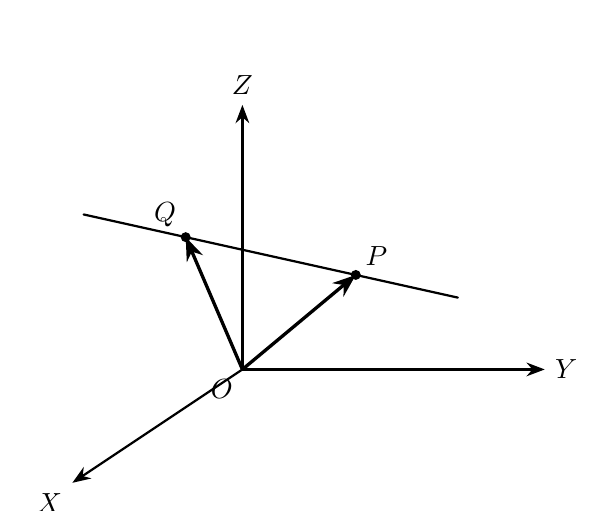
\begin{tikzpicture}[>=Stealth, scale=1.2, line cap=round, line join=round]
  % Coordinates axes
  \draw[->, thick] (0, 0) -- (-1.8, -1.2) node[below left] {$X$};
  \draw[->, thick] (0, 0) -- (3.2, 0) node[right] {$Y$};
  \draw[->, thick] (0, 0) -- (0, 2.8) node[above] {$Z$};
  \node[below left] at (0,0) {$O$};

  % Points P and Q
  \coordinate (P) at (1.2, 1.0);
  \coordinate (Q) at (-0.6, 1.4);

  % Draw OP and OQ
  \draw[->, very thick] (0,0) -- (P) node[midway, right=1pt] {};
  \draw[->, very thick] (0,0) -- (Q) node[midway, left=1pt] {};

  % Draw line through P and Q
  \draw[thick] ($(P)!-0.6!(Q)$) -- ($(P)!1.6!(Q)$);

  \fill (P) circle (1.5pt) node[above right] {$P$};
  \fill (Q) circle (1.5pt) node[above left] {$Q$};
\end{tikzpicture}
\caption*{圖 1-1}\label{fig:b6s-1-1}
\end{figure}

在 $\mathbb{R}^3$ 中，可作圖如圖 1-1。

關於一般 $\mathbb{R}^n$ 中的“距離”以及相關的“垂直”等觀念，就不擬作深入討論了。

\subsubsection*{丙、線性相關與線性無關}\label{subsec:b6s-1-1-c}

為了計算的方便，從本段開始我們一律不區分點與向量，而一律以圓括弧“$(\quad)$”表點和向量。

讓我們從一個例子開始：

\begin{example}\label{ex:b6s-1-4}
$\mathbb{R}^3$ 中二向量 $\vec{OP}=(-1, 2, 1), \vec{OQ}=(3, -1, 3)$，試描出 $3\vec{OP}+2\vec{OQ}$ 的終點 $R$。
\end{example}

\paragraph{【解】}
在等價看法下
\[ R = (-3, 6, 3) + (6, -2, 6) = (3, 4, 9) \]

\begin{figure}[H]
\centering
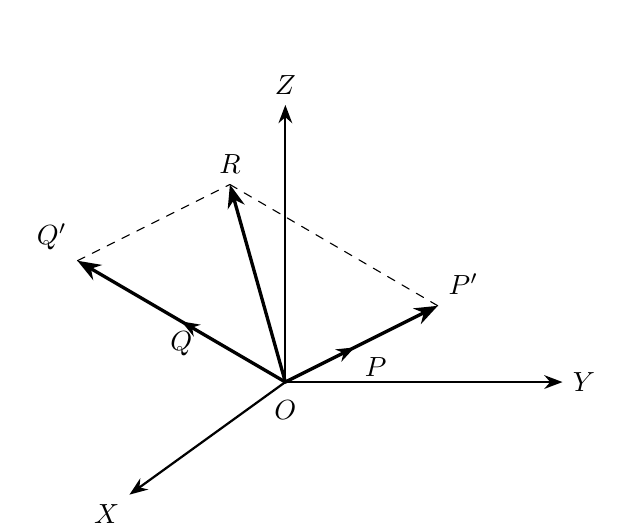
\begin{tikzpicture}[>=Stealth, scale=1.1, line cap=round, line join=round]
  % Axes
  \draw[->, thick] (0, 0) -- (-1.8, -1.3) node[below left] {$X$};
  \draw[->, thick] (0, 0) -- (3.2, 0) node[right] {$Y$};
  \draw[->, thick] (0, 0) -- (0, 3.2) node[above] {$Z$};
  \node[below] at (0, -0.1) {$O$};

  % Vectors P, Q, P', Q', R
  \coordinate (P) at (0.8, 0.4);
  \coordinate (Q) at (-1.2, 0.7);
  \coordinate (Pp) at ($(0,0)!2.2!(P)$);
  \coordinate (Qp) at ($(0,0)!2.0!(Q)$);
  \coordinate (R) at ($(Pp)+(Qp)$);

  \draw[->, thick] (0,0) -- (P) node[below right] {$P$};
  \draw[->, thick] (0,0) -- (Q) node[below] {$Q$};
  \draw[->, very thick] (0,0) -- (Pp) node[above right] {$P'$};
  \draw[->, very thick] (0,0) -- (Qp) node[above left] {$Q'$};
  \draw[->, very thick] (0,0) -- (R) node[above] {$R$};

  \draw[dashed] (Pp) -- (R);
  \draw[dashed] (Qp) -- (R);
\end{tikzpicture}
\caption*{圖 1-2}\label{fig:b6s-1-2}
\end{figure}

讀者或能直觀地看出，在上例中 $R$ 是落在由 $O, P, Q$ 三點所決定的平面上。並且可以算出 $\vec{Q'R}=\vec{OP'}, \vec{P'R}=\vec{OQ'}$。反之，對 $O, P, Q$ 三點所決定平面上任一點如 $R$ 者，可以自 $R$ 聯平行線分別平行於 $\vec{OQ}$ 及 $\vec{OP}$，設分別交於 $Q', P'$，令 $\alpha = \frac{\overline{OP'}}{\overline{OP}}, \beta = \frac{\overline{OQ'}}{\overline{OQ}}$ 則 $\vec{OR} = \alpha\vec{OP} + \beta\vec{OQ}$，或作 $\vec{OR} - \alpha\vec{OP} - \beta\vec{OQ} = \vect{0}$。

例 4 提示了四件事：
\begin{enumerate}[label=(\alph*), leftmargin=2em]
  \item 對任意實數 $\alpha, \beta$，$\alpha\vec{OP} + \beta\vec{OQ}$ 均在 $O, P, Q$ 所決定的平面上。
  \item $O, P, Q$ 所張平面上任一點均可表作 $\alpha\vec{OP} + \beta\vec{OQ}$ 的形式。
  \item 對這平面上任一點 $R$，可找到實數 $\alpha, \beta, \gamma$ 使得 $\alpha\vec{OP} + \beta\vec{OQ} + \gamma\vec{OR} = \vect{0}$。
  \item 性質 (c) 並不對空間中其他點適合。
\end{enumerate}

現在要規定幾個重要名詞：設 $\vect{a}_1, \vect{a}_2, \dots, \vect{a}_m$ 為 $\mathbb{R}^n$ 中向量。

\begin{definition}\label{def:b6s-1-1}
\begin{enumerate}[label=(\roman*), leftmargin=2em]
  \item 設向量 $\vect{b}$ 在 $\mathbb{R}^n$ 中可表作 $\vect{b}=\sum_{i=1}^m \lambda_i \vect{a}_i$（$\lambda_i$ 均為實數），則稱 $\vect{b}$ 為 $\vect{a}_1, \vect{a}_2, \dots, \vect{a}_m$ 的\textbf{線性組合}。
  \item $\sigma = \left\{ \vect{b} \;\middle|\; \vect{b}=\sum_{i=1}^m \lambda_i \vect{a}_i, \lambda_i \text{ 為實數} \right\}$ 稱為由 $\vect{a}_1, \vect{a}_2, \dots, \vect{a}_m$ 所\textbf{張成的子空間}。
\end{enumerate}
\end{definition}

由 (a) 式，$\vec{OP}, \vec{OQ}$ 所張成的子空間（在點與向量的等價看法下）就是過原點的一個平面，由 $\vec{OP}$ 所張成的子空間便是過原點的一條直線，顯然原點 $O$ 在這些子空間上。

\begin{discussion}\label{disc:b6s-1-1}
向量 $\vect{u}=(-1, 2, 1), \vect{v}=(3, -1, 3)$ 展成的子空間設為 $\sigma$。令 $\vec{OP}=(x, y, z)$ 為子空間（平面）上一點，則存在實數 $\alpha, \beta$ 使得
\[ \vec{OP}=(x, y, z) = \alpha \vect{u} + \beta \vect{v} = (-\alpha+3\beta, 2\alpha-\beta, \alpha+3\beta) \]
即
\begin{equation}
\left\{\begin{aligned}
-\alpha + 3\beta &= x \\
2\alpha - \beta &= y \\
\alpha + 3\beta &= z
\end{aligned}\right. \label{eq:b6s-1-1-6}
\end{equation}
由消去法解得
\begin{equation}
7x + 6y - 5z = 0 \label{eq:b6s-1-1-7}
\end{equation}
即 $x, y, z$ 滿足 (7) 式。反之若 $\vec{OP}=(x, y, z)$ 滿足 (7) 式，則由 (6) 式求 $\alpha, \beta$：
\begin{enumerate}[label=(\roman*), leftmargin=2em]
  \item (6) 式可解，因為
  \[ \begin{vmatrix} -1 & 3 & x \\ 2 & -1 & y \\ 1 & 3 & z \end{vmatrix} = 7x + 6y - 5z = 0 \]
  \item 對此一組解 $\alpha, \beta$，顯然
  \[ \vec{OP} = (x, y, z) = \alpha\vect{u} + \beta\vect{v} \]
\end{enumerate}
這說明了 (7) 式為點 $\vec{OP}$ 在 $\vect{u}, \vect{v}$ 所展成子空間的充要條件，通稱為一平面的方程式。\hfill$\#$
\end{discussion}

\paragraph{附註：}雖然用一個數表示點的位置，古希臘時代就已經開始用了，並且到紀元 1637 年，笛卡爾把這個觀念推到二維和三維的情形，但直到十九世紀數學家 Cayley 和 Grassmann 才發現到“為什麼要停在三個數上呢？”這才開始了 $n$ 維空間的研究。

\subsubsection*{作業 1}\label{hw:b6s-1-1}
設 $\vect{u}, \vect{v}$ 同上，
\begin{enumerate}[label=(\roman*), leftmargin=2em]
  \item $\vect{w}=(1, 1, 0)$，試問 $\vect{u}, \vect{v}, \vect{w}$ 所展成的子空間是否為一平面？
  \item 若 $\vect{w}$ 改成 $(3, 4, 9)$ 又如何？
\end{enumerate}

\begin{definition}\label{def:b6s-1-2}
設 $\vect{a}_1, \vect{a}_2, \dots, \vect{a}_m$ 為 $\mathbb{R}^n$ 中向量，若存在非盡為 0 的實數 $\lambda_1, \lambda_2, \dots, \lambda_m$ 使得
\begin{equation}
\sum_{i=1}^m \lambda_i \vect{a}_i = \vect{0} \label{eq:b6s-1-1-8}
\end{equation}
則稱 $\vect{a}_1, \vect{a}_2, \dots, \vect{a}_m$ 為\textbf{線性相關}。反之，對一組 $\lambda_1, \lambda_2, \dots, \lambda_m$，若 $\sum_{i=1}^m \lambda_i \vect{a}_i = \vect{0}$ 僅當 $\lambda_1=\lambda_2=\dots=\lambda_m=0$ 時成立，此時 $\vect{a}_1, \vect{a}_2, \dots, \vect{a}_m$ 稱作\textbf{線性無關}。
\end{definition}

由第三冊的討論，$\mathbb{R}^3$ 中可以找到三個線性無關的向量，而且 $\mathbb{R}^3$ 中線性無關向量的最大數是 3，並且任何向量均可唯一表成三個線性無關向量的線性組合，也就是說三個線性無關的向量形成 $\mathbb{R}^3$ 的一組基底，並且任何四向量在 $\mathbb{R}^3$ 中均線性相關。在 $\mathbb{R}^n$ 中我們有類似的性質，試條列數項於后，作為參考。至於嚴格的證明雖是不難但較繁瑣，就略去不提。讀者只要將 $\mathbb{R}^3$ 的情形弄清楚，以憑藉它來推想。
\begin{enumerate}[label=\Roman*., leftmargin=2.5em]
  \item $\mathbb{R}^n$ 中線性無關向量之最大數恰好是 $n$，並且 $\mathbb{R}^n$ 中任一向量均可表為 $n$ 個線性無關向量的線性組合。這樣一組 $n$ 個線性無關的向量稱作一組\textbf{基底}（顯然 $\vect{0}$ 不在內）。
  \item $\mathbb{R}^n$ 中的任 $k$ 個線性無關向量 $\vect{a}_1, \vect{a}_2, \dots, \vect{a}_k$，$k < n$，都可另找到 $\vect{a}_{k+1}, \dots, \vect{a}_n$，使得 $\vect{a}_1, \vect{a}_2, \dots, \vect{a}_n$ 為線性無關。
\end{enumerate}

\paragraph{註：}對一個基底，固定一點為基準點，I 中所說即此組基底形成一 $\mathbb{R}^n$ 中的座標系。

本書將恆以 $\vect{e}_1, \vect{e}_2, \dots, \vect{e}_n$ 為基底，原點 $O$ 為基準點形成的座標系來討論。

\begin{example}\label{ex:b6s-1-5}
$\mathbb{R}^4$ 中試問 $\vect{u}_1=(1, 2, 0, 1), \vect{u}_2=(-1, 1, 1, 0), \vect{u}_3=(0, -1, 2, -3), \vect{u}_4=(3, 1, -1, 2)$ 是線性相關還是線性無關？
\end{example}

\paragraph{【解】}
設存在 $\lambda_1, \lambda_2, \lambda_3, \lambda_4$ 使得
\[ \lambda_1\vect{u}_1 + \lambda_2\vect{u}_2 + \lambda_3\vect{u}_3 + \lambda_4\vect{u}_4 = \vect{0} \]
即
\begin{equation}
\left\{\begin{aligned}
\lambda_1 - \lambda_2 \phantom{+ 2\lambda_3} + 3\lambda_4 &= 0 \\
2\lambda_1 + \lambda_2 - \lambda_3 + \lambda_4 &= 0 \\
\lambda_2 + 2\lambda_3 - \lambda_4 &= 0 \\
\lambda_1 \phantom{+ \lambda_2} - 3\lambda_3 + 2\lambda_4 &= 0
\end{aligned}\right. \label{eq:b6s-1-1-9}
\end{equation}
若此聯立方程組有一組非全為 0 的解，則 $\vect{u}_1, \vect{u}_2, \vect{u}_3, \vect{u}_4$ 為線性相關，否則為線性無關。用消去法解之，發現此方程組只有一組 $\lambda_1=\lambda_2=\lambda_3=\lambda_4=0$ 的解，故 $\vect{u}_1, \vect{u}_2, \vect{u}_3, \vect{u}_4$ 為線性無關。\hfill$\#$

\begin{example}\label{ex:b6s-1-6}
在上例中以 $\vect{u}_1, \vect{u}_2, \vect{u}_3, \vect{u}_4$ 的線性組合來表 $\vect{a}=(2, 2, -1, 6)$。
\end{example}

\paragraph{【解】}
此題在於找 $\lambda_1, \lambda_2, \lambda_3, \lambda_4$ 使得
\[ \lambda_1\vect{u}_1 + \lambda_2\vect{u}_2 + \lambda_3\vect{u}_3 + \lambda_4\vect{u}_4 = \vect{a} \]
由向量相等的意義得聯立方程：
\begin{equation}
\left\{\begin{aligned}
\lambda_1 - \lambda_2 \phantom{+ 2\lambda_3} + 3\lambda_4 &= 2 \\
2\lambda_1 + \lambda_2 - \lambda_3 + \lambda_4 &= 2 \\
\lambda_2 + 2\lambda_3 - \lambda_4 &= -1 \\
\lambda_1 \phantom{+ \lambda_2} - 3\lambda_3 + 2\lambda_4 &= 6
\end{aligned}\right. \label{eq:b6s-1-1-10}
\end{equation}
用消去法得 $\lambda_1=1, \lambda_2=2, \lambda_3=-1, \lambda_4=1$。故
\[ \vect{a} = \vect{u}_1 + 2\vect{u}_2 - \vect{u}_3 + \vect{u}_4 \]\hfill$\#$

上例中 $\lambda_1, \lambda_2, \lambda_3, \lambda_4$ 不難解得，但一般情形如何？請就以下作業試驗。

\subsubsection*{作業 2}\label{hw:b6s-1-2}
$\vect{u}_1, \vect{u}_2, \vect{u}_3$ 同上，問能否用三向量的線性組合表 $\vect{a}=(1, 1, -\frac{1}{2}, 3)$？這說明什麼？

\subsubsection*{作業 3}\label{hw:b6s-1-3}
$\vect{u}_1, \vect{u}_2, \vect{u}_3$ 同上，$\vect{u}_4$ 改為 $(3, 2, 1, -1)$ 則四向量能否表 $\vect{a}=(1, 1, -\frac{1}{2}, 3)$？為什麼？

\paragraph{註：}關於一般 $n$ 元一次聯立方程的公式解，請參考 § I-8 的討論。至於消去法，讀者應已很熟練了。

\begin{theorem}\label{thm:b6s-1-1}
$\vect{a}_1, \vect{a}_2, \dots, \vect{a}_m$ 為線性相關，則必其中某一向量可寫為其餘諸向量的線性組合，即在其餘諸向量所決定的子空間上。
\end{theorem}

\begin{proof}[【證明】]
由假設，可找到非盡為 0 的 $\lambda_1, \lambda_2, \dots, \lambda_m$ 使得 (8) 式成立。經重新安排指標可假設 $\lambda_1 \ne 0$，則
\[ \lambda_1 \vect{a}_1 = - \sum_{i=2}^m \lambda_i \vect{a}_i \]
即
\[ \vect{a}_1 = \sum_{i=2}^m \left(-\dfrac{\lambda_i}{\lambda_1}\right) \vect{a}_i \]
\end{proof}\hfill$\#$

\subsubsection*{作業 4}\label{hw:b6s-1-4}
試證 $\vect{e}_1, \vect{e}_2, \dots, \vect{e}_n$ 在 $\mathbb{R}^n$ 中形成一組基底。（即證：\textcircled{1} $\vect{e}_1, \vect{e}_2, \dots, \vect{e}_n$ 線性無關。\textcircled{2} $\mathbb{R}^n$ 中任一向量均可寫成此 $n$ 個向量的線性組合。）

\subsubsection*{作業 5}\label{hw:b6s-1-5}
在 $\mathbb{R}^5$ 中，將 $\vect{a}=(4, 61, -13, 7, 9)$ 寫作其第一至第五個單位向量的線性組合。此寫法是否唯一？說明之。

\subsubsection*{作業 6}\label{hw:b6s-1-6}
$\mathbb{R}^3$ 中設 $\vect{a}_1=(1, 2, 1), \vect{a}_2=(2, -1, 3), \vect{a}_3=(-1, 1, 1)$。
\begin{enumerate}[label=(\roman*), leftmargin=2em]
  \item 試證 $\vect{a}_1, \vect{a}_2, \vect{a}_3$ 線性無關。
  \item 若 $\vect{a}=(3, 4, 2)$，試將 $\vect{a}$ 寫作 $\vect{a}_1, \vect{a}_2, \vect{a}_3$ 的線性組合。
  \item 試證不可能找到一向量 $\vect{a}_4$，使得 $\vect{a}_1, \vect{a}_2, \vect{a}_3, \vect{a}_4$ 線性無關。
\end{enumerate}

\subsubsection*{作業 7}\label{hw:b6s-1-7}
$\mathbb{R}^3$ 中，試證不可能找到向量 $\vect{a}_1, \vect{a}_2$，使得 $\mathbb{R}^3$ 中任何一向量均可寫成它們的線性組合。

\subsubsection*{作業 8}\label{hw:b6s-1-8}
設 $\vect{a}_1=(1, 2, 4), \vect{a}_2=(-1, 1, 3)$ 試找一 $\vect{a}_3$ 使得 $\vect{a}_1, \vect{a}_2, \vect{a}_3$ 為線性無關。（提示：方法很多，這種 $\vect{a}_3$ 也有無限個，只要找一向量不在 $\vect{a}_1, \vect{a}_2$ 所展成的子空間即可。）

\begin{definition*}[*]\label{def:b6s-1-dim}
設 $\sigma$ 為 $\mathbb{R}^n$ 的一個子空間，$\sigma$ 中線性無關向量的最大數 $m$ 稱作 $\sigma$ 的\textbf{維數}，$\sigma$ 稱作 \textbf{$m$ 維子空間}\footnote{【原書註】：嚴格說，此定義不完全，有一個問題存在：此所謂的線性無關向量的最大數 $m$，會不會因兩次不同的向量取法而有不同？即是否有此 $m$ 存在？事實上與丙段 I, II 的情形一樣，下面幾個性質成立：
\begin{enumerate}[label=(\roman*), leftmargin=2em]
  \item 此 $m$ 存在。
  \item 任一 $\sigma$ 中的向量均可唯一寫成 $\sigma$ 中一組給定 $m$ 個線性無關向量的線性組合。
  \item 對 $\sigma$ 中任 $k$ 個線性無關的向量（$k < m$），可找到 $m-k$ 個向量使此 $m$ 個向量線性無關。
\end{enumerate}
因此我們也往往稱一個 $m$ 維子空間內，$m$ 個線性無關向量為一組基底。}。例如論例 1 之 $\sigma$ 為二維子空間。
\end{definition*}

\subsubsection*{作業 9}\label{hw:b6s-1-9}
\begin{enumerate}[label=(\roman*), leftmargin=2em]
  \item 試求作業 1 中兩子空間的維數。
  \item 試求由 $\vect{u}=(-1, 2, 1)$ 與 $\vect{v}=(2, -4, -2)$ 所展成子空間方程式。（提示：為二方程式所組成。）
  \item 將 (ii) 中的直線用 (1) 式表出。
\end{enumerate}

從定義我們可以顯然看出，$\mathbb{R}^3$ 中三個向量若是線性相關，則三向量所決定的子空間必為一平面或為一直線或竟為 $O$ 點，即其維數必小於 3。

\subsubsection*{丁、$\mathbb{R}^n$ 中的線性映射與方陣}\label{subsec:b6s-1-1-d}

$\mathbb{R}^n$ 顯然是人類最不難了解的空間，從 $\mathbb{R}^n$ 到 $\mathbb{R}^m$ 的函數當然也是最有趣的了。可是從 $\mathbb{R}^n$ 到 $\mathbb{R}^m$ 的函數一般來說是相當複雜的，其最有用的，也是人類最能處理的，就是一次的，也就是我們所稱\textbf{線性映射}了。我們將看出它與多元一次聯立方程組是息息相關的。為了討論方便，本書將僅討論 $n=m$ 的情形\footnote{【原書註】：二次方程也是人類較能了解的，但到了三次以上就非常艱深了。}。

在第四冊 § 1-3, § 1-4, § 1-5 內我們已經探討了 $\mathbb{R}^2$ 上的線性映射和它們的方陣表示。那邊特別舉出（平面上）剛性運動，強調某種線性映射相當於一種運動。或者我們更可以把線性映射看作經過一個三稜鏡或是放大鏡或是近視眼鏡所成的像來想像。

\begin{example}\label{ex:b6s-1-7}
設 $f(x_1, x_2) = (\sqrt{3}x_1 - x_2, x_1 + \sqrt{3}x_2)$，試求點 $O(0, 0)$，$A(1, 1), B(0, 2), C(-1, 1)$ 的像點 $O, A', B', C'$ 的座標，又 $O, A, B, C$ 形成一正方形的四端點，是否 $O, A', B', C'$ 亦形成一正方形的四端點？
\end{example}

\paragraph{【解】}
$A'=(\sqrt{3}-1, 1+\sqrt{3})$，$B'=(-2, 2\sqrt{3})$，$C'=(-\sqrt{3}-1, -1+\sqrt{3})$。
又驗證 $\vec{OA'} \cdot \vec{OC'} = \vec{A'B'} \cdot \vec{B'C'} = \vec{B'C'} \cdot \vec{OC'} = 0$
且 $\overline{OA'} = \overline{A'B'} = \overline{B'C'} = \overline{OC'} = 2\sqrt{2}$。
所以 $O, A', B', C'$ 形成正方形的端點，而且邊界映射到相應邊界，（$\mathbb{R}^2$ 中線性映射將直線映到直線）。只是邊長改變了兩倍，位置也不一樣了，反時針轉了 $\dfrac{\pi}{6}$，見圖 1-3。\hfill$\#$

\begin{figure}[H]
\centering
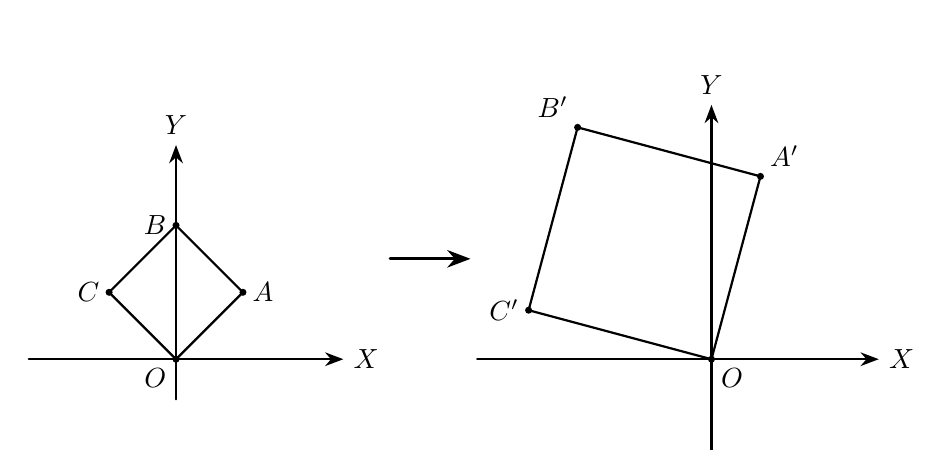
\begin{tikzpicture}[>=Stealth, scale=0.85, line cap=round, line join=round]
  % Left figure
  \begin{scope}[shift={(0,0)}]
    \draw[->, thick] (-2.2, 0) -- (2.5, 0) node[right] {$X$};
    \draw[->, thick] (0, -0.6) -- (0, 3.2) node[above] {$Y$};
    \node[below left] at (0,0) {$O$};

    \coordinate (O) at (0,0);
    \coordinate (A) at (1,1);
    \coordinate (B) at (0,2);
    \coordinate (C) at (-1,1);

    \draw[thick] (O) -- (A) -- (B) -- (C) -- cycle;
    \fill (O) circle (1.5pt);
    \fill (A) circle (1.5pt) node[right] {$A$};
    \fill (B) circle (1.5pt) node[left] {$B$};
    \fill (C) circle (1.5pt) node[left] {$C$};
  \end{scope}

  % Mapping arrow
  \draw[->, very thick] (3.2, 1.5) -- (4.4, 1.5);

  % Right figure
  \begin{scope}[shift={(8,0)}]
    \draw[->, thick] (-3.5, 0) -- (2.5, 0) node[right] {$X$};
    \draw[->, thick] (0, -1.5) -- (0, 3.8) node[above] {$Y$};
    \node[below right] at (0,0) {$O$};

    \coordinate (O) at (0,0);
    \coordinate (Ap) at ({sqrt(3)-1}, {1+sqrt(3)});
    \coordinate (Bp) at (-2, {2*sqrt(3)});
    \coordinate (Cp) at ({-sqrt(3)-1}, {-1+sqrt(3)});

    \draw[thick] (O) -- (Ap) -- (Bp) -- (Cp) -- cycle;
    \fill (O) circle (1.5pt);
    \fill (Ap) circle (1.5pt) node[above right] {$A'$};
    \fill (Bp) circle (1.5pt) node[above left] {$B'$};
    \fill (Cp) circle (1.5pt) node[left] {$C'$};
  \end{scope}
\end{tikzpicture}
\caption*{圖 1-3}\label{fig:b6s-1-3}
\end{figure}

\subsubsection*{作業 10}\label{hw:b6s-1-10}
上例 $f$ 的方陣表示為何？是否為一剛性運動？

\subsubsection*{作業 11}\label{hw:b6s-1-11}
試求正方形 $OABC$（包括邊界和內部）的映像為何？說明之。

\paragraph{注意：}關於列出一線性映射之方陣及一點座標而求像點，我們可將點座標寫在左邊，方陣寫在右邊，然後以點座標的列乘以方陣的行即得。就如：
\[ (x_1, x_2) \begin{pmatrix} a_{11} & a_{12} \\ a_{21} & a_{22} \end{pmatrix} \]
相乘有如：
\[ (\longrightarrow) \begin{pmatrix} \Big\downarrow & \Big\downarrow \end{pmatrix} \]

\begin{example}\label{ex:b6s-1-8}
設 $f$ 的方陣表示為 $\begin{pmatrix} 2 & 1 \\ 1 & -1 \end{pmatrix}$，$O, A, B, C$ 同上，$A', B', C'$ 分別為 $f$ 下的像點，求其座標。四邊形 $OA'B'C'$ 是否成一正方形？
\end{example}

\paragraph{【解】}
\begin{align*}
A' &= (1, 1) \begin{pmatrix} 2 & 1 \\ 1 & -1 \end{pmatrix} = (2+1, 1-1) = (3, 0) \\
B' &= (0, 2) \begin{pmatrix} 2 & 1 \\ 1 & -1 \end{pmatrix} = (2, -2) \\
C' &= (-1, 1) \begin{pmatrix} 2 & 1 \\ 1 & -1 \end{pmatrix} = (-2+1, -1-1) = (-1, -2)
\end{align*}
$\vec{OA'} \cdot \vec{OC'} = -3 \ne 0$。
故此四邊形非正方形。由於線性映射把向量映至向量，也就是說，把相平行的線段映至相平行的線段，所以四邊形 $OA'B'C'$ 為平行四邊形。當然這也可以由直接檢視向量 $\vec{OA'}=\vec{C'B'}, \vec{A'B'}=\vec{OC'}$ 得知。見圖 1-4。\hfill$\#$

\begin{example}\label{ex:b6s-1-9}
設 $f$ 之方陣表示為 $\begin{pmatrix} 1 & -2 \\ 2 & -4 \end{pmatrix}$，$O, A, B, C$ 同上，求 $A', B', C'$ 之座標。
\end{example}

\paragraph{【解】}
同上計算得
\[ A'=(3, -6), \quad B'=(4, -8), \quad C'=(1, -2) \]
且
\[ \begin{vmatrix} 3 & -6 & 1 \\ 4 & -8 & 1 \\ 1 & -2 & 1 \end{vmatrix} = 0 \]
三點共線。見圖 1-5。\hfill$\#$

\begin{figure}[H]
\centering
\begin{minipage}[c]{0.48\textwidth}
\centering
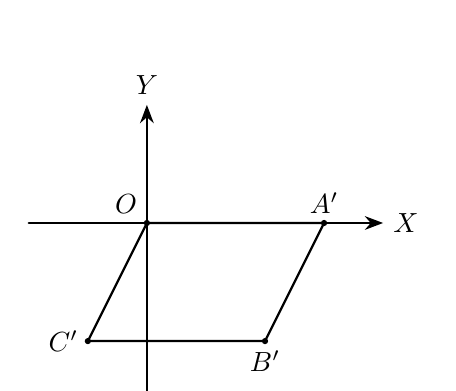
\begin{tikzpicture}[>=Stealth, scale=0.75, line cap=round, line join=round]
  \draw[->, thick] (-2.0, 0) -- (4.0, 0) node[right] {$X$};
  \draw[->, thick] (0, -3.0) -- (0, 2.0) node[above] {$Y$};
  \node[above left] at (0,0) {$O$};

  \coordinate (O) at (0,0);
  \coordinate (Ap) at (3,0);
  \coordinate (Bp) at (2,-2);
  \coordinate (Cp) at (-1,-2);

  \draw[thick] (O) -- (Ap) -- (Bp) -- (Cp) -- cycle;
  \fill (O) circle (1.5pt);
  \fill (Ap) circle (1.5pt) node[above] {$A'$};
  \fill (Bp) circle (1.5pt) node[below] {$B'$};
  \fill (Cp) circle (1.5pt) node[left] {$C'$};
\end{tikzpicture}
\caption*{圖 1-4}\label{fig:b6s-1-4}
\end{minipage}\hfill
\begin{minipage}[c]{0.48\textwidth}
\centering
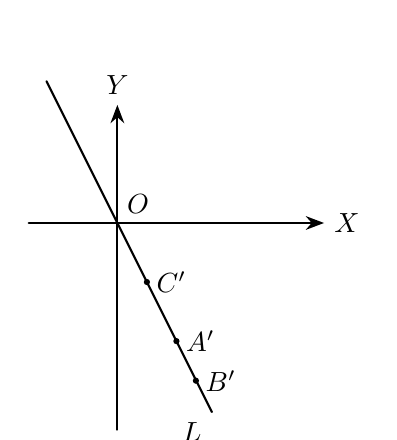
\begin{tikzpicture}[>=Stealth, scale=0.75, line cap=round, line join=round]
  \draw[->, thick] (-1.5, 0) -- (3.5, 0) node[right] {$X$};
  \draw[->, thick] (0, -3.5) -- (0, 2.0) node[above] {$Y$};
  \node[above right] at (0,0) {$O$};

  % Line L: 2x + y = 0
  \draw[thick] (-1.2, 2.4) -- (1.6, -3.2) node[below left] {$L$};

  \coordinate (Cp) at (0.5, -1.0);
  \coordinate (Ap) at (1.0, -2.0);
  \coordinate (Bp) at (1.33, -2.67);

  \fill (Cp) circle (1.5pt) node[right] {$C'$};
  \fill (Ap) circle (1.5pt) node[right] {$A'$};
  \fill (Bp) circle (1.5pt) node[right] {$B'$};
\end{tikzpicture}
\caption*{圖 1-5}\label{fig:b6s-1-5}
\end{minipage}
\end{figure}

\subsubsection*{作業 12}\label{hw:b6s-1-12}
試證在例 9 中，整個 $\mathbb{R}^2$ 平面映成到直線 $L$。

從上三例約略可以窺見，平面上一般的線性映射是相當複雜的也不像剛性運動那樣規則。一般 $\mathbb{R}^n$ 到 $\mathbb{R}^n$ 的線性映射亦可類似定義，不過在 $n \ge 3$ 時其構造又自然複雜多了。本章主要目的在闡明線性映射及其方陣之表示與行列式有關的基本重要問題。

\begin{definition}\label{def:b6s-1-3}
設有一函數 $f: \mathbb{R}^n \longrightarrow \mathbb{R}^n$，若 $(y_1, y_2, \dots, y_n)$ 表示點 $(x_1, x_2, \dots, x_n)$ 在 $f$ 下的像點，即 $f(x_1, x_2, \dots, x_n) = (y_1, y_2, \dots, y_n)$，而知存在 $n^2$ 個實數 $a_{ij}$，$i, j = 1, 2, \dots, n$ 使得
\begin{equation}
y_j = \sum_{i=1}^n a_{ij} x_i \qquad j = 1, 2, \dots, n \label{eq:b6s-1-1-11}
\end{equation}
對每一點 $(x_1, x_2, \dots, x_n)$ 均成立，則稱 $f$ 為 $\mathbb{R}^n$ 到 $\mathbb{R}^n$ 的一個\textbf{線性映射}。
\end{definition}

通常 $f$ 可記為
\[ f(x_1, x_2, \dots, x_n) = \left( \sum_{i=1}^n a_{i1} x_i, \sum_{i=1}^n a_{i2} x_i, \dots, \sum_{i=1}^n a_{in} x_i \right) \]
這 $n^2$ 個實數 $a_{ij}$ 形成一個正方形的矩陣，稱作 \textbf{$n$ 階方陣}，記為
\begin{equation}
\begin{pmatrix}
a_{11} & a_{12} & \dots & a_{1n} \\
a_{21} & a_{22} & \dots & a_{2n} \\
\dots & \dots & \dots & \dots \\
a_{n1} & a_{n2} & \dots & a_{nn}
\end{pmatrix} \quad \text{或簡記作 } (a_{ij}) \label{eq:b6s-1-1-12}
\end{equation}
其中 $a_{ij}$ 稱為原素，各橫列稱作方陣之\textbf{列}，各縱行稱作方陣之\textbf{行}，$a_{ij}$ 係位於第 $i$ 列第 $j$ 行的原素，$i$ 稱作列指標，$j$ 稱作行指標。方陣之各原素均有一定位置，兩方陣僅在對應位置之各原素均相等時，始稱相等。顯然 $\mathbb{R}^n$ 到 $\mathbb{R}^n$ 的線性映射與 $n$ 階方陣之間有一一對應的關係，即兩線性映射為相等當且僅當對應之方陣相等。相應於每一線性映射有一方陣，對每一方陣可找唯一線性映射使彼之方陣表示即為此給定方陣。

以方陣之第 $i$ 列中各原素作分量而得之向量
\begin{equation}
\vect{a}_i = (a_{i1}, a_{i2}, \dots, a_{in}) \qquad i=1, 2, \dots, n \label{eq:b6s-1-1-13}
\end{equation}
稱作方陣之第 $i$ 個\textbf{列向量}，以第 $j$ 行的各原素為分量而得之向量
\begin{equation}
\vect{a}_j^* = (a_{1j}, a_{2j}, \dots, a_{nj}) \qquad j=1, 2, \dots, n \label{eq:b6s-1-1-14}
\end{equation}
稱作方陣之第 $j$ 個\textbf{行向量}。

\begin{example}\label{ex:b6s-1-10}
設 $f(x_1, x_2, x_3) = (3x_1 - 2x_2 + x_3, x_1 + x_2 - x_3, x_1 + 2x_2 - 2x_3)$ 問 $f$ 是否線性映射？若是，其方陣表示為何？又求 $P(1, 2, 1), Q(2, 1, -1), R(3, 0, -3)$ 相應之像點 $P', Q', R'$ 的座標。又知 $P, Q, R$ 三點在一直線上（因為 $\vec{OR} = \vec{OP} + 2\vec{PQ}$）問 $P', Q', R'$ 是否也在同一直線上？
\end{example}

\paragraph{【解】}
$f$ 之方陣表示為
\[ \begin{pmatrix} 3 & 1 & 1 \\ -2 & 1 & 2 \\ 1 & -1 & -2 \end{pmatrix} \]
\begin{align*}
P' &= (1, 2, 1) \begin{pmatrix} 3 & 1 & 1 \\ -2 & 1 & 2 \\ 1 & -1 & -2 \end{pmatrix} = (3-4+1, 1+2-1, 1+4-2) = (0, 2, 3)
\end{align*}
同理 $Q' = (3, 4, 6)$，$R' = (6, 6, 9)$。
且 $\vec{OR'} = \vec{OP'} + 2\vec{P'Q'}$，故 $P', Q', R'$ 在同一直線上。

另一種看法是：$P', Q', R'$ 在同一直線上的充要條件是 $\vec{P'Q'}$ 與 $\vec{P'R'}$ 線性相關，這是極易判定的。\hfill$\#$

\subsubsection*{作業 13}\label{hw:b6s-1-13}
試證線段 $OP$ 在 $f$ 下的映像為線段 $OP'$。

\subsubsection*{作業 14}\label{hw:b6s-1-14}
設 $f: \mathbb{R}^3 \longrightarrow \mathbb{R}^3$ 定為 $f(x_1, x_2, x_3) = (x_1 + 2x_2^2, -x_3, x_2 - x_3)$，
$g: \mathbb{R}^3 \longrightarrow \mathbb{R}^3$ 定為 $g(x_1, x_2, x_3) = (x_1 x_2, x_1 + x_3, x_2 - x_3)$。
試問 $f, g$ 是否為線性映射？說明之。

\subsubsection*{作業 15}\label{hw:b6s-1-15}
$f$ 如例 10 所示，設 $S=(3, 3, 0)$ 我們知 $\vec{OP} = \vec{QS}$（亦即 $OP \parallel QS$）試證 $OP' \parallel Q'S'$，$S'=f(S)$，又試證 $\vec{OP'} = \vec{Q'S'}$。

線性映射顯然把原點映至原點，作業 13 與 15 的性質事實上對一般線性映射均成立。線性映射原是一個把 $\mathbb{R}^n$ 的點指向其像點的函數，我們也可將之看作是從向量映到向量的函數，關係如下：
\[ f(P)=P' \text{ 可記為 } f(\vec{OP}) = \vec{OP'} \]
也就是在點與向量的等價關係下，把線性映射 $f: \mathbb{R}^n \longrightarrow \mathbb{R}^n$ 也看作是由 $\mathbb{R}^n$ 中的向量映到 $\mathbb{R}^n$ 中向量的函數。這樣，對 $\mathbb{R}^n$ 中向量 $\vect{a}$，$f(\vect{a})$ 就有意義了。即設 $\vect{a}=\vec{OA}$，則 $f(\vect{a}) = f(A)$（見作業 13）。在此種等價關係下，容易驗證 $\mathbb{R}^n$ 上的線性映射 $f$ 滿足：
\begin{enumerate}[label=\Roman*., leftmargin=2.5em]
  \item 對所有向量 $\vect{a}, \vect{b}$ 和實數 $\alpha, \beta$ 均成立：
  \begin{equation}
  f(\alpha\vect{a} + \beta\vect{b}) = \alpha f(\vect{a}) + \beta f(\vect{b}) \label{eq:b6s-1-1-15}
  \end{equation}
  \item $f$ 把直線映至直線。
  \item 設 $f$ 如 (11) 給定，$\vect{e}_1, \vect{e}_2, \dots, \vect{e}_n$ 如前，則
  \begin{equation}
  f(\vect{e}_i) = \sum_{j=1}^n a_{ij} \vect{e}_j \label{eq:b6s-1-1-16}
  \end{equation}
  （請注意 (16) 與 (11) 中指標次序不同）
  \item $f$ 把線性相關向量映至線性相關向量。
\end{enumerate}

\paragraph{注意：}$f$ 不一定將線性無關向量映至線性無關向量，參考例 9。

\subsubsection*{作業 16}\label{hw:b6s-1-16}
試證對 $\mathbb{R}^n$ 中任意四點 $P_1, P_2, Q_1, Q_2$ 若有 $\vec{P_1P_2} = \vec{Q_1Q_2}$ 則 $f(\vec{P_1P_2}) = f(\vec{Q_1Q_2})$（提示：由 (11) 式或 (15) 式）。

\subsubsection*{作業 17}\label{hw:b6s-1-17}
試證明上面 I, II, III, IV 諸性質。

\subsubsection*{習題 I-1}\label{sec:b6s-ex1-1}

\begin{enumerate}[label=\arabic*., leftmargin=2em]
  \item $\mathbb{R}^3$ 中二向量 $\left(\dfrac{1}{2}, -3, 5\right)$ 與 $(1, -6, 10)$ 是否平行？

  \stepcounter{enumi}
  \item[\textbf{*2.}] 過兩點 $\vec{OP}=(a_1, a_2, \dots, a_n), \vec{OQ}=(b_1, b_2, \dots, b_n)$ 的直線方程式可表為（亦即向量表示法）
  \phantomsection\label{note:b6s-ch1-p19-l-eq}%
  \[ L = \{ \vec{OP} + \lambda\vec{PQ} : \lambda \text{ 為任意實數} \}\footnotemark \]
  \footnotetext{【原書校訂】：原書此處印作「$L=\{\vec{OP}+\lambda\vec{OQ}\}$」，據後文「$x_i = a_i + \lambda(b_i - a_i)$」校訂為方向向量 $\vec{PQ}$。}
  即 $(x_1, x_2, \dots, x_n)$ 為 $L$ 上一點的充要條件是存在一實數 $\lambda$，使得
  \[ x_i = a_i + \lambda(b_i - a_i) \qquad i=1, 2, \dots, n \]
  即
  \[ \dfrac{x_i - a_i}{b_i - a_i} = \lambda \qquad i=1, 2, \dots, n \]
  其中 $\lambda$ 隨點 $(x_1, x_2, \dots, x_n)$ 而變。所以直線方程式的另一種寫法為：
  \[ \dfrac{x_1 - a_1}{c_1} = \dfrac{x_2 - a_2}{c_2} = \dots = \dfrac{x_n - a_n}{c_n} \]
  $(c_1, c_2, \dots, c_n)$ 為與直線平行的一個向量，此稱直線的比例式。試求 $\mathbb{R}^3$ 中，過兩點 $(-5, 3, 2), (2, -3, 6)$ 的直線方程式的兩種寫法。\\
  （註：我們還可將 $\mathbb{R}^3$ 中直線方程式寫作兩平面方程式的交點，以後再作說明，請參考第三冊 § 4-8 之習題 8。）

  \item 設 $\vect{a}_1=(7, 1, -3), \vect{a}_2=(1, -5, 2)$ 試找 $\mathbb{R}^3$ 中一與 $\vect{a}_1, \vect{a}_2$ 線性無關的向量，並敘述理由。

  \item 如上題，找 $\mathbb{R}^3$ 中一點，使不在 $\vect{a}_1, \vect{a}_2$ 所決定的平面，並請敘述理由。

  \item 求 $\mathbb{R}^3$ 中由 $\vect{u}=(1, 2, -1), \vect{v}=(-1, 2, 2)$ 所決定平面之方程式表示。

  \item 設 $\mathbb{R}^3$ 中三點 $P_1=(1, 3, 6), P_2=(3, 4, -3), P_3=(2, 1, 5)$ 試決定下列向量：
  \begin{enumerate}[label=(\Alph*)]
    \item $\vec{OP_1} + \vec{OP_2} - \vec{OP_3}$
    \item $7\vec{OP_1} - 2\vec{OP_2} - 3\vec{OP_3}$
  \end{enumerate}

  \item 設 $P_1=(1, 1, 1), P_2=(0, 1, 1), P_3=(1, -1, 0)$ 為 $\mathbb{R}^3$ 中三點，$\vec{OP_4} = x\vec{OP_1} + y\vec{OP_2} + z\vec{OP_3}$。
  \begin{enumerate}[label=(\alph*)]
    \item 試決定 $\vec{OP_4}$ 的分量。
    \item 若 $P_4=O$ 試證 $x=y=z=0$ 為唯一解。
    \item $P_4=(1, 2, 3)$ 試求 $x, y, z$。
  \end{enumerate}

  \item 設 $P_1=(1, 1, 1, 0), P_2=(0, 1, 1, 1), P_3=(1, 1, 0, 0)$ 為 $\mathbb{R}^4$ 中三個點，且 $P_4 = x P_1 + y P_2 + z P_3$。
  \begin{enumerate}[label=(\alph*)]
    \item 試決定 $P_4$ 的分量。
    \item 若 $P_4=O$，試證 $x=y=z=0$。
    \item 若 $P_4=(1, 5, 3, 4)$ 試求 $x, y, z$。
    \item 請問可選擇到 $x, y, z$ 使得 $P_4=(1, 2, 3, 4)$ 可表成 $P_4 = x P_1 + y P_2 + z P_3$ 嗎？
  \end{enumerate}

  \stepcounter{enumi}
  \item[\textbf{*9.}] 設 $P=(x_1, x_2, \dots, x_n), Q=(y_1, y_2, \dots, y_n)$ 為 $\mathbb{R}^n$ 中二點，試問：
  \begin{enumerate}[label=(\alph*)]
    \item 如何描述 $QP$？
    \item $QP$ 與 $PQ$ 的關係如何？
  \end{enumerate}

  \item $P, Q$ 如上題，又如
  \[ PQ = \{ (z_1, z_2, \dots, z_n) : \text{存在一實數 } \lambda, \text{使得 } z_i = x_i + \lambda(y_i - x_i), i=1, 2, \dots, n \} \]
  則：
  \begin{enumerate}[label=(\alph*)]
    \item 如何描述 $QP$？
    \item $PQ$ 與 $QP$ 之關係如何？
  \end{enumerate}

  \item 設 $P, Q$ 為 $\mathbb{R}^5$ 中二點，且 $\vec{PQ} = (2, -3, -1, 0, 4)$。
  \begin{enumerate}[label=(\alph*)]
    \item 若 $P=(-1, 1, 0, -3, 7)$ 試求 $Q$ 點。
    \item 若 $Q=(-2, 3, -3, 2, 1)$ 試求 $P$ 點。
  \end{enumerate}

  \item 設 $P, Q$ 為 $\mathbb{R}^4$ 中二點，當 $P, Q$ 為下列各種情形時，試求 $\vec{PQ}, 2\vec{PQ}$ 及 $\vec{PQ}$ 方向的單位向量：
  \begin{enumerate}[label=(\alph*)]
    \item $P=(1, 0, 1, 1) \quad Q=(0, 1, 1, 0)$
    \item $P=(3, 2, 1, 0) \quad Q=(0, 1, 2, 3)$
  \end{enumerate}

  \item 設 $P, Q, R, S$ 為 $\mathbb{R}^3$ 中四點，若 $\vec{PQ} = \vec{RS}$，試問線段 $PQ$ 與 $RS$ 之間的關係如何？四邊形 $PQSR$ 的形狀如何？

  \item
  \begin{enumerate}[label=(\alph*)]
    \item 設 $P, Q, R, S$ 為 $\mathbb{R}^3$ 中四點，則如何可知四邊形 $PQRS$ 為一平行四邊形？
    \item 若 $P=(1, 0, -1), Q=(0, 1, 1), R=(1, 1, 0)$ 且 $PQRS$ 為一平行四邊形，試求 $S$ 點。
  \end{enumerate}

  \item 當 $\vect{a}_1, \vect{a}_2, \vect{a}_3$ 為下列各種情形時，試問 $\vect{a}_1, \vect{a}_2, \vect{a}_3$ 是否線性無關？
  \begin{enumerate}[label=(\alph*)]
    \item $\vect{a}_1=(1, 0, 1), \vect{a}_2=(0, 0, 1), \vect{a}_3=(1, 1, 1)$
    \item $\vect{a}_1=(1, -1, 2), \vect{a}_2=(7, 2, -1), \vect{a}_3=(-19, -8, 7)$
    \item $\vect{a}_1=(0, 2, -1), \vect{a}_2=(3, 0, -2), \vect{a}_3=(3, 2, 3)$
  \end{enumerate}

  \stepcounter{enumi}
  \item[\textbf{*16.}] 設 $\vect{a}_1,$ $\vect{a}_2,$ $\dots,$ $\vect{a}_n$ 為線性無關，且 $\vect{a}_{n+1}$ 非 $\vect{a}_1,$ $\vect{a}_2,$ $\dots,$ $\vect{a}_n$ 的線性組合。試證 $\vect{a}_1,$ $\vect{a}_2,$ $\dots,$ $\vect{a}_{n+1}$ 為線性無關。

  \item 試求二向量 $(a, b), (c, d)$ 為線性無關的充要條件。

  \item 試求向量 $(a_1, a_2, a_3), (b_1, b_2, b_3), (c_1, c_2, c_3)$ 為線性無關的充要條件。

  \item 試證 $\vect{a}=(3, 1, 5), \vect{b}=(-2, 1, 3), \vect{c}=(19, -2, 0)$ 三向量為線性相關，並以 $\vect{a}, \vect{b}$ 的線性組合表 $\vect{c}$。

  \item 試求由向量 $\left(2, -\dfrac{1}{2}, 3\right)$ 過點 $(1, -1, 1)$ 所決定的直線的方程式。

  \item $f(x_1, x_2, x_3) = (3x_1 - x_2 + 2x_3, x_1 - 3x_2 - x_3, 2x_1 + x_2 + 3x_3)$ 試求 $f$ 之方陣表示。設 $\vect{e}_1, \vect{e}_2, \vect{e}_3$ 如前為 $\mathbb{R}^3$ 的一組基底，試求 $f(\vect{e}_i)$ 以 $\vect{e}_1, \vect{e}_2, \vect{e}_3$ 的線性組合表之。

  \stepcounter{enumi}
  \item[\textbf{*22.}] 求 $f: \mathbb{R}^n \longrightarrow \mathbb{R}^n, f(x_1, x_2, \dots, x_n) = (x_1, x_2, \dots, x_n)$ 的方陣表示。

  \item
  \begin{enumerate}[label=(\alph*)]
    \item $f: \mathbb{R}^3 \longrightarrow \mathbb{R}^3, f(x_1, x_2, x_3) = (2x_2, x_1 + 1, x_2 + x_3)$ 是否為一線性映射？
    \item $f(r, \theta) = (r\cos\theta, r\sin\theta)$ 又如何？
    \item $f(x, y, z) = (3x, 2, 5y + z)$ 又如何？
  \end{enumerate}

  \item 設 $f: \mathbb{R}^2 \longrightarrow \mathbb{R}^2$ 為線性映射，並滿足 $f(1, 1) = (3, -1), f(-2, 3) = (6, -2)$，試求 $f(3, 4), f(0, 6)$，已知 $(1, 1), (-2, 3), (3, 4), (0, 6)$ 形成一正方形的四頂點，試問四像點所成的四邊形圖形如何？繪圖示之。

  \item 設 $f: \mathbb{R}^2 \longrightarrow \mathbb{R}^2$ 為線性映射，$\vect{a}, \vect{b}$ 為 $\mathbb{R}^2$ 中二線性無關向量，若 $f(\vect{a}), f(\vect{b})$ 平行試證任一平行四邊形的像點形成一線段或一點。

  \item 設 $f: \mathbb{R}^3 \longrightarrow \mathbb{R}^3$ 為線性映射，$P_1, P_2, P_3$ 三點共線，試證 $f(P_1), f(P_2), f(P_3)$ 三點共線。

  \item 設 $f: \mathbb{R}^4 \longrightarrow \mathbb{R}^4$ 為一函數，且 $f(x_1, x_2, x_3, x_4) = (x_1 + x_3 + x_4, x_1 + x_2 + x_4, x_1 + x_2 + x_3, x_2 + x_3 + x_4)$。
  \begin{enumerate}[label=(\alph*)]
    \item 試問 $f$ 是否為一線性映射？若是其方陣表示為何？
    \item 求點 $P=(1, 2, 1, 1), Q=(3, 3, 3, 3), R=(1, 0, 0, 1)$ 相應之像點 $P', Q', R'$\phantomsection\label{note:b6s-ch1-p22-ex28-s}\footnote{【原書註記】：原書此處印作「求像點 $P', Q', R', S'$」，惟題目僅給出三點 $P, Q, R$，故像點應為 $P', Q', R'$。}的座標。
  \end{enumerate}

  \item 設 $f: \mathbb{R}^3 \longrightarrow \mathbb{R}^3$ 為線性映射，且 $f(\vect{e}_1) = \vect{e}_1 + \vect{e}_3, f(\vect{e}_2) = 2\vect{e}_1 - \vect{e}_2 + \vect{e}_3, f(\vect{e}_3) = 7\vect{e}_1 - 3\vect{e}_2$。
  \begin{enumerate}[label=(\alph*)]
    \item 試計算 $f(3\vect{e}_1 - 4\vect{e}_2 + \vect{e}_3)$。
    \item 試求 $f$ 之方陣表示。
  \end{enumerate}

\end{enumerate}

\subsection{行列式與有向面積、體積}\label{sec:b6s-1-2}
\resetsectcounters

\subsubsection*{甲、引言}\label{subsec:b6s-1-2-a}

第一冊討論聯立方程組時，事實上已引進了行列式的觀念。而後在討論行列式與體積，求兩直線交點問題和線性映射時又曾分別在第三、四冊裏介紹了更多行列式的應用。這裏我們嚐試在不繁瑣的原則下，對它作一個系統的整理和介紹。

長度，面積和體積的度量，不僅是數學上也是物理世界重要的課題。平面上平行四邊形的面積可視為一切面積度量的基礎；空間裏平行六面體的體積亦可視為一切體積度量的基礎。許多實際問題經過轉化後變成爲度量更高維抽象空間的“體積”，如何度量一個 $\mathbb{R}^n$ 的“平行體”的“體積”就是一個很值得處理的問題。此外，多元一次聯立方程組的問題需要一種一般的方法來處理，這是與行列式息息相關的。本節將分析二維和三維空間裏平行四邊形和平行六面體的一些基本性質，冀圖從中導出行列式的一般形式。

\subsubsection*{乙、n 維平行體的體積}\label{subsec:b6s-1-2-b}

$\mathbb{R}^2$ 中由兩向量 $\vect{u}, \vect{v}$ 張出的平行四邊形可以用下面點集表示：
\begin{equation}
\{ \vec{OP} : \vec{OP} = \alpha\vect{u} + \beta\vect{v}, 0 \le \alpha, \beta \le 1 \} \label{eq:b6s-1-2-1}
\end{equation}
（在點與向量在形式上的等價關係下來看）

$\mathbb{R}^3$ 中也有類似定義。這觀念可以推至 $\mathbb{R}^n$ 中：

\begin{definition}\label{def:b6s-1-4}
$\mathbb{R}^n$ 中 $n$ 個線性無關的向量 $\vect{a}_1, \vect{a}_2, \dots, \vect{a}_n$，今考慮集合
\begin{equation}
\tau = \left\{ \vec{OP} : \vec{OP} = \sum_{i=1}^n \lambda_i \vect{a}_i, 0 \le \lambda_i \le 1, i=1, 2, \dots, n \right\} \label{eq:b6s-1-2-2}
\end{equation}
$\tau$ 稱為向量 $\vect{a}_1, \vect{a}_2, \dots, \vect{a}_n$ 所張出的 \textbf{$n$ 維平行體}。
\end{definition}

\begin{example}\label{ex:b6s-1-11}
試繪出 $\mathbb{R}^3$ 中由 $\vect{u}=(-2, 5, 1), \vect{v}=(-3, 1, \frac{3}{2}), \vect{w}=(-2, 3, \frac{7}{2})$ 所決定的平行六面體。
\end{example}

\paragraph{【解】}
見圖 2-1。\hfill$\#$

\begin{figure}[H]
\centering
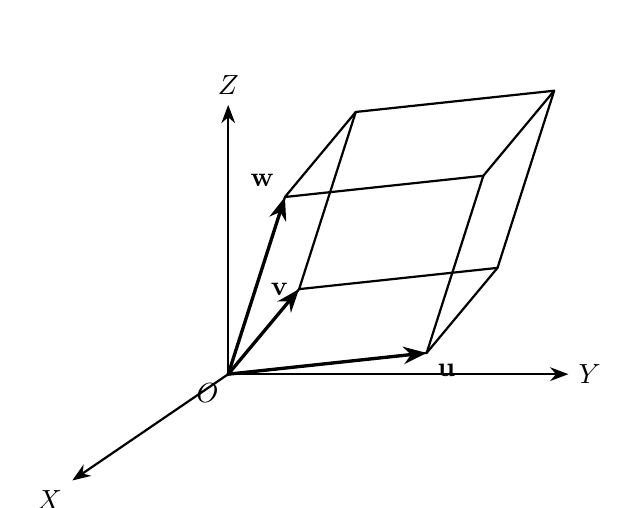
\begin{tikzpicture}[>=Stealth, scale=0.9, line cap=round, line join=round]
  % Axes
  \draw[->, thick] (0, 0) -- (-2.2, -1.5) node[below left] {$X$};
  \draw[->, thick] (0, 0) -- (4.8, 0) node[right] {$Y$};
  \draw[->, thick] (0, 0) -- (0, 3.8) node[above] {$Z$};
  \node[below left] at (0,0) {$O$};

  % Vectors u, v, w
  % Let u = (-2, 5, 1) -> visual coords: u_x = -0.7*(-2) + 0.8*(5) etc.
  % We project (x,y,z) to (y - 0.7*x, z - 0.5*x)
  % For visual clarity, choose attractive 3d oblique projection:
  \coordinate (O) at (0,0);
  \coordinate (U) at (2.8, 0.3); % vector u
  \coordinate (V) at (1.0, 1.2); % vector v
  \coordinate (W) at (0.8, 2.5); % vector w

  \coordinate (UV) at ($(U)+(V)$);
  \coordinate (UW) at ($(U)+(W)$);
  \coordinate (VW) at ($(V)+(W)$);
  \coordinate (UVW) at ($(U)+(V)+(W)$);

  % Draw base
  \draw[thick] (O) -- (U);
  \draw[thick] (O) -- (V);
  \draw[thick] (U) -- (UV);
  \draw[thick] (V) -- (UV);

  % Draw vertical edges
  \draw[thick] (O) -- (W);
  \draw[thick] (U) -- (UW);
  \draw[thick] (V) -- (VW);
  \draw[thick] (UV) -- (UVW);

  % Draw top face
  \draw[thick] (W) -- (UW) -- (UVW) -- (VW) -- cycle;

  % Arrows for u, v, w
  \draw[->, very thick] (O) -- (U) node[below right] {$\vect{u}$};
  \draw[->, very thick] (O) -- (V) node[left] {$\vect{v}$};
  \draw[->, very thick] (O) -- (W) node[above left] {$\vect{w}$};
\end{tikzpicture}
\caption*{圖 2-1}\label{fig:b6s-2-1}
\end{figure}

今考慮一個二階方陣，分別以 $\vect{a}_1=(a_{11}, a_{12}), \vect{a}_2=(a_{21}, a_{22})$ 表其第一、第二列向量，此方陣可記為 $\begin{bmatrix} \vect{a}_1 \\ \vect{a}_2 \end{bmatrix}$。我們來複習一下第三冊 § 3-7 中的演算，以決定由 $\vect{a}_1, \vect{a}_2$ 所張出的平行四邊形的面積 $V$。取 $\vect{u} = \dfrac{\vect{a}_1}{|\vect{a}_1|}$ 為 $\vect{a}_1$ 的方向，則顯然如圖 2-2 所示：

\begin{figure}[H]
\centering
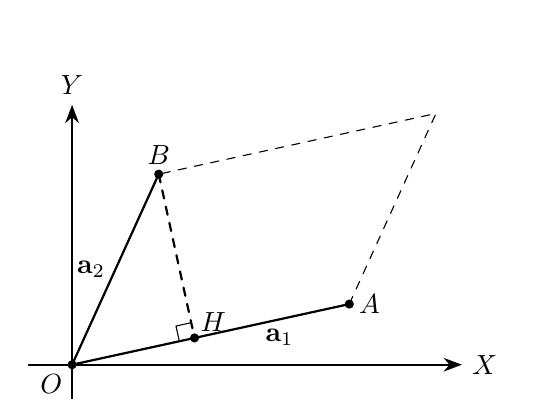
\begin{tikzpicture}[>=Stealth, scale=1.1, line cap=round, line join=round]
  \draw[->, thick] (-0.5, 0) -- (4.5, 0) node[right] {$X$};
  \draw[->, thick] (0, -0.5) -- (0, 3.0) node[above] {$Y$};
  \node[below left] at (0,0) {$O$};

  \coordinate (O) at (0,0);
  \coordinate (A) at (3.2, 0.7);
  \coordinate (B) at (1.0, 2.2);
  \coordinate (D) at ($(A)+(B)$);
  % Orthogonal projection of B onto line OA
  \coordinate (H) at ($(O)!(B)!(A)$);

  \draw[thick] (O) -- (A);
  \node[below] at ($(H)!0.55!(A)$) {$\vect{a}_1$};
  \draw[thick] (O) -- (B) node[midway, left] {$\vect{a}_2$};
  \draw[dashed] (A) -- (D) -- (B);
  \draw[dashed, thick] (B) -- (H);

  \fill (O) circle (1.5pt);
  \fill (A) circle (1.5pt) node[right] {$A$};
  \fill (B) circle (1.5pt) node[above] {$B$};
  \fill (H) circle (1.5pt) node[above right, inner sep=2pt] {$H$};

  % Right angle mark at H
  \draw ($(H)!0.18cm!(B)$) -- ($($(H)!0.18cm!(B)$)+($(H)!0.18cm!(O)$)-(H)$) -- ($(H)!0.18cm!(O)$);
\end{tikzpicture}
\caption*{圖 2-2}\label{fig:b6s-2-2}
\end{figure}

\begin{equation}
V = \overline{OA} \cdot \overline{HB} = |\vect{a}_1| \cdot |\vect{a}_2 - (\vect{a}_2 \cdot \vect{u})\vect{u}| \label{eq:b6s-1-2-3}
\end{equation}
由第三冊 § 3-7 的計算得
\[ V = |a_{11} a_{22} - a_{12} a_{21}| = \left| \begin{vmatrix} a_{11} & a_{12} \\ a_{21} & a_{22} \end{vmatrix} \right| \text{ 的絕對值} \]
即方陣 $\begin{bmatrix} \vect{a}_1 \\ \vect{a}_2 \end{bmatrix}$ 的行列式的絕對值。我們曾以 $|\vect{a}_1 \wedge \vect{a}_2|$ 表示。為了討論方便，有時用 $\det \begin{bmatrix} \vect{a}_1 \\ \vect{a}_2 \end{bmatrix}$ 或 $|a_{ij}|$ 表 $\begin{vmatrix} a_{11} & a_{12} \\ a_{21} & a_{22} \end{vmatrix}$。若是除去絕對值的符號，$\det \begin{bmatrix} \vect{a}_1 \\ \vect{a}_2 \end{bmatrix}$ 所代表的就是稱作\textbf{有向面積}，記作 $V(\vect{a}_1, \vect{a}_2)$。顯然，$V(\vect{a}_2, \vect{a}_1) = -V(\vect{a}_1, \vect{a}_2)$ 此式表明 $V(\vect{a}_1, \vect{a}_2)$ 的值因向量選取的次序而易號。當然，負面積原是沒有意義的，這樣的安排是為著方向的考慮和討論的方便。

三維空間中平行六面體的體積又如何求法？（請參閱第三冊 § 3-7，又見同冊第五章作業 8 和習題 5-2 我們把這問題重作詳述。）設 $\vect{a}_1=(a_{11}, a_{12}, a_{13}), \vect{a}_2=(a_{21}, a_{22}, a_{23}), \vect{a}_3=(a_{31}, a_{32}, a_{33})$ 為 $\mathbb{R}^3$ 中三向量，今考慮三者所張出平行六面體：如圖 2-3，自 $O$ 分別取向量 $\vect{a}_1, \vect{a}_2, \vect{a}_3$，先計算由 $\vect{a}_1, \vect{a}_2$ 所張出 $\square OADB$ 的面積，再乘以高度 $\overline{CE}$ 便得到所求平行六面體的體積了。今仿上段求法，計算 $\square OADB$ 面積如下（見圖 2-3）：

取 $\vect{u}=\dfrac{\vect{a}_1}{|\vect{a}_1|}$\phantomsection\label{note:b6s-ch1-p24-u}\footnote{【原書校訂】：原書此處印作「$\vect{u}=\frac{\vect{a}}{|\vect{a}|}$」，漏下標 $1$，據上下文校訂為「$\vect{u}=\frac{\vect{a}_1}{|\vect{a}_1|}$」。}，則

$\vect{a}_2$ 在 $\vect{u}$ 方向的投影
\[ \vec{OH} = (\vect{a}_2 \cdot \vect{u})\vect{u} \]
故
\[ \vec{HB} = \vec{OB} - \vec{OH} = \vect{a}_2 - (\vect{a}_2 \cdot \vect{u})\vect{u} \]
\begin{align*}
(\square OADB \text{ 的面積})^2 &= |\vect{a}_2 - (\vect{a}_2 \cdot \vect{u})\vect{u}|^2 |\vect{a}_1|^2 \\
&= \left[ |\vect{a}_2|^2 - \left(\dfrac{\vect{a}_2 \cdot \vect{a}_1}{|\vect{a}_1|}\right)^2 \right] |\vect{a}_1|^2 \\
&= |\vect{a}_1|^2 |\vect{a}_2|^2 - (\vect{a}_1 \cdot \vect{a}_2)^2
\end{align*}
設 $\vect{v} = \dfrac{\vect{a}_2 - (\vect{a}_2 \cdot \vect{u})\vect{u}}{|\vect{a}_2 - (\vect{a}_2 \cdot \vect{u})\vect{u}|}$ 為 $\vec{HB}$ 的方向（單位向量），則向量 $\vec{OC}$ 在 $\square OADB$ 上的投影 $\vec{OE}$ 可表為
\[ \vec{OE} = (\vect{a}_3 \cdot \vect{u})\vect{u} + (\vect{a}_3 \cdot \vect{v})\vect{v} \]
且
\[ \vec{EC} = \vect{a}_3 - (\vect{a}_3 \cdot \vect{u})\vect{u} - (\vect{a}_3 \cdot \vect{v})\vect{v}\footnotemark \]
\footnotetext{【原書註】：因為 $\vec{EC}\cdot\vect{u} = \vec{EC}\cdot\vect{v} = 0$，故在 $\vec{EC}$ 與平面上任一向量均垂直，即 $\vec{EC} \perp \text{平面 } OADB$。又 $\vect{a}_3 \cdot \vec{EC} = |\vect{a}_3|^2 - (\vect{a}_3\cdot\vect{u})^2 - (\vect{a}_3\cdot\vect{v})^2 = \vec{EC}\cdot\vec{EC} = |\vec{EC}|^2 > 0$，又且 $\vect{a}_3 \cdot \vec{EC} = |\vect{a}_3|\,|\vec{EC}|\cos\theta$（$\theta$ 為二向量交角），即 $|\vec{EC}| = |\vect{a}_3|\cos\theta$，表示 $\vec{EC} \perp \vec{OE}$（因 $\vec{EC}$ 為 $\vect{a}_3$ 在直線 $EC$ 上的投影）。又 $0 \le \theta \le \frac{\pi}{2}$，所以 $\vec{EC}=\vect{a}_3$ 在直線 $EC$ 上的投影。（$0 \le \theta \le \frac{\pi}{2}$ 除去了“$-\vec{EC}=\vect{a}_3$ 在直線 $EC$ 上的投影”這一可能性）}

\begin{figure}[H]
\centering
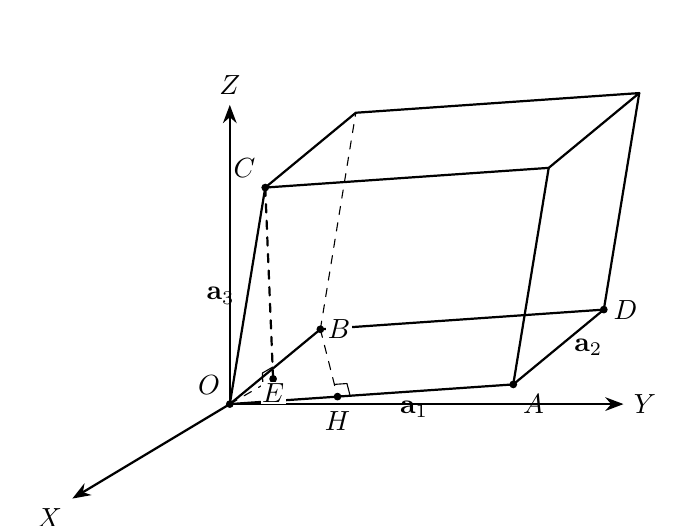
\begin{tikzpicture}[>=Stealth, scale=1.0, line cap=round, line join=round]
  % Axes
  \draw[->, thick] (0, 0) -- (-2.0, -1.2) node[below left] {$X$};
  \draw[->, thick] (0, 0) -- (5.0, 0) node[right] {$Y$};
  \draw[->, thick] (0, 0) -- (0, 3.8) node[above] {$Z$};
  \node[above left] at (0,0) {$O$};

  \coordinate (O) at (0,0);
  \coordinate (A) at (3.6, 0.25); % a1
  \coordinate (B) at (1.15, 0.95); % a2
  \coordinate (D) at ($(A)+(B)$);
  \coordinate (C) at (0.45, 2.75); % a3

  \coordinate (Ap) at ($(A)+(C)$);
  \coordinate (Bp) at ($(B)+(C)$);
  \coordinate (Dp) at ($(D)+(C)$);

  % Base parallelogram
  \draw[thick] (O) -- (A);
  \node[below] at ($(O)!0.65!(A)$) {$\vect{a}_1$};
  \draw[thick] (O) -- (B);
  \draw[thick] (A) -- (D) node[midway, right=2pt] {$\vect{a}_2$};
  \draw[thick] (B) -- (D);

  % Top parallelogram
  \draw[thick] (C) -- (Ap) -- (Dp) -- (Bp) -- cycle;

  % Vertical edges
  \draw[thick] (O) -- (C) node[midway, left=1pt] {$\vect{a}_3$};
  \draw[thick] (A) -- (Ap);
  \draw[dashed] (B) -- (Bp);
  \draw[thick] (D) -- (Dp);

  % Points H (foot of B on OA) and E (foot of C on base plane)
  \path (O) -- (A) coordinate[pos=0.38] (H);
  \coordinate (E) at (0.55, 0.32);

  \draw[dashed] (B) -- (H);
  \draw[dashed, thick] (C) -- (E);
  \draw[dashed] (O) -- (E);

  % Right-angle mark at H (HB perp OA)
  \draw ($(H)!0.16cm!(B)$) -- ($($(H)!0.16cm!(B)$)+($(H)!0.16cm!(A)$)-(H)$) -- ($(H)!0.16cm!(A)$);
  % Right-angle mark at E (CE perp OE)
  \draw ($(E)!0.15cm!(C)$) -- ($($(E)!0.15cm!(C)$)+($(E)!0.15cm!(O)$)-(E)$) -- ($(E)!0.15cm!(O)$);

  \fill (O) circle (1.4pt);
  \fill (A) circle (1.4pt) node[below right] {$A$};
  \fill (B) circle (1.4pt) node[right=2pt, fill=white, inner sep=0.5pt] {$B$};
  \fill (D) circle (1.4pt) node[right] {$D$};
  \fill (C) circle (1.4pt) node[above left] {$C$};
  \fill (H) circle (1.4pt) node[below=2pt] {$H$};
  \fill (E) circle (1.4pt) node[right=2pt, below=1pt, fill=white, inner sep=0.5pt] {$E$};
\end{tikzpicture}
\caption*{圖 2-3}\label{fig:b6s-2-3}
\end{figure}

所求平行六面體的體積 $V$ 可以計算如下：
\begin{align*}
V^2 &= \left[ |\vect{a}_1|^2 |\vect{a}_2|^2 - (\vect{a}_1 \cdot \vect{a}_2)^2 \right] |\vect{a}_3 - (\vect{a}_3 \cdot \vect{u})\vect{u} - (\vect{a}_3 \cdot \vect{v})\vect{v}|^2 \\
&= \left[ |\vect{a}_1|^2 |\vect{a}_2|^2 - (\vect{a}_1 \cdot \vect{a}_2)^2 \right] \left[ |\vect{a}_3|^2 - (\vect{a}_3 \cdot \vect{u})^2 - (\vect{a}_3 \cdot \vect{v})^2 \right] \\
&= \left[ |\vect{a}_1|^2 |\vect{a}_2|^2 - (\vect{a}_1 \cdot \vect{a}_2)^2 \right] \left[ |\vect{a}_3|^2 - \dfrac{(\vect{a}_3 \cdot \vect{a}_1)^2}{|\vect{a}_1|^2} - \dfrac{((\vect{a}_3 \cdot \vect{a}_2) - (\vect{a}_2 \cdot \vect{u})(\vect{a}_3 \cdot \vect{u}))^2 |\vect{a}_1|^2}{|\vect{a}_1|^2 |\vect{a}_2|^2 - (\vect{a}_1 \cdot \vect{a}_2)^2} \right] \\
&= |\vect{a}_1|^2 \cdot |\vect{a}_2|^2 \cdot |\vect{a}_3|^2 - (\vect{a}_1 \cdot \vect{a}_2)^2 |\vect{a}_3|^2 - (\vect{a}_3 \cdot \vect{a}_1)^2 |\vect{a}_2|^2 \\
&\quad - (\vect{a}_3 \cdot \vect{a}_2)^2 |\vect{a}_1|^2 + 2(\vect{a}_1 \cdot \vect{a}_3)(\vect{a}_3 \cdot \vect{a}_2)(\vect{a}_2 \cdot \vect{a}_1) \\
&= (a_{11}^2 + a_{12}^2 + a_{13}^2)(a_{21}^2 + a_{22}^2 + a_{23}^2)(a_{31}^2 + a_{32}^2 + a_{33}^2) \\
&\quad - (a_{11}a_{21} + a_{12}a_{22} + a_{13}a_{23})^2 (a_{31}^2 + a_{32}^2 + a_{33}^2) \\
&\quad - (a_{11}a_{31} + a_{12}a_{32} + a_{13}a_{33})^2 (a_{21}^2 + a_{22}^2 + a_{23}^2) \\
&\quad - (a_{21}a_{31} + a_{22}a_{32} + a_{23}a_{33})^2 (a_{11}^2 + a_{12}^2 + a_{13}^2) \\
&\quad + 2(a_{21}a_{31} + a_{22}a_{32} + a_{23}a_{33})(a_{11}a_{21} + a_{12}a_{22} + a_{13}a_{23})(a_{11}a_{31} + a_{12}a_{32} + a_{13}a_{33}) \\
&= (a_{11}a_{22}a_{33} + a_{13}a_{21}a_{32} + a_{12}a_{23}a_{31} - a_{13}a_{22}a_{31} - a_{12}a_{21}a_{33} - a_{11}a_{23}a_{32})^2 \\
&= \begin{vmatrix}
a_{11} & a_{12} & a_{13} \\
a_{21} & a_{22} & a_{23} \\
a_{31} & a_{32} & a_{33}
\end{vmatrix}^2
\end{align*}
\[ V = \left| \det \begin{bmatrix} \vect{a}_1 \\ \vect{a}_2 \\ \vect{a}_3 \end{bmatrix} \right| \]
若去掉絕對值的符號，$\det \begin{bmatrix} \vect{a}_1 \\ \vect{a}_2 \\ \vect{a}_3 \end{bmatrix}$ 所代表的就是稱作此平行六面體的\textbf{有向體積}，記作 $V(\vect{a}_1, \vect{a}_2, \vect{a}_3)$。變換 $\vect{a}_1, \vect{a}_2, \vect{a}_3$ 中任兩列向量的次序，則相差一負號。例如 $V(\vect{a}_3, \vect{a}_2, \vect{a}_1) = -V(\vect{a}_1, \vect{a}_2, \vect{a}_3)$。這三向量 $\vect{a}_1, \vect{a}_2, \vect{a}_3$ 選取的次序與物理上所指左手定則或右手定則有關，作為定向之用，也是 $\det \begin{bmatrix} \vect{a}_1 \\ \vect{a}_2 \\ \vect{a}_3 \end{bmatrix}$ 值為正或為負的來源，在這裏就不細述了。

雖然上述這種求體積的方法已經比從純粹座標幾何的角度來處理要精簡得多，可仍然是十分繁瑣。在求一般 $\mathbb{R}^n$ 中 $n$ 維平行體的“體積”時（確切地說，推廣 $\mathbb{R}^3$ 中平行六面體的體積算法——底部平行四邊形的面積乘以高度——到一般 $\mathbb{R}^n$ 的情形時）這樣的計算顯然不是一個理想的方法。

我們嚐試列舉並分析一下 $\mathbb{R}^2$ 中的平行四邊形有向面積與 $\mathbb{R}^3$ 中平行六面體有向體積的一些基本性質，希望能抽出一些作為行列式的定義，用以求取一般 $\mathbb{R}^n$ 中 $n$ 維平行體的體積。

令 $\vect{a}, \vect{b}, \vect{c}$ 為 $\mathbb{R}^2$ 中三向量，以 $V(\vect{a}, \vect{b})$ 表 $\vect{a}, \vect{b}$ 所張平行四邊形之有向面積（亦即容許有負值的面積）。下面幾個性質可以從圖上清楚看出：
\begin{enumerate}[label=\Roman*., leftmargin=2.5em]
  \item $V(\lambda\vect{a}, \vect{b}) = \lambda V(\vect{a}, \vect{b})$ 對任意實數 $\lambda$ 均滿足。見圖 2-4。
  
  \begin{figure}[H]
  \centering
  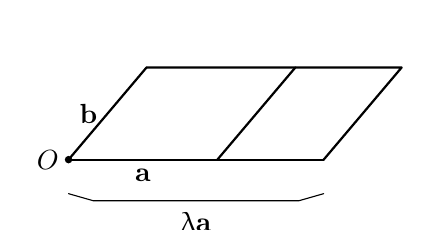
\begin{tikzpicture}[>=Stealth, scale=0.9, line cap=round, line join=round]
    \coordinate (O) at (0,0);
    \coordinate (A) at (2.1, 0);
    \coordinate (B) at (1.1, 1.3);
    \coordinate (AB) at ($(A)+(B)$);
    \coordinate (lA) at (3.6, 0);
    \coordinate (lAB) at ($(lA)+(B)$);

    \draw[thick] (O) -- (lA);
    \draw[thick] (O) -- (B) node[midway, left] {$\vect{b}$};
    \draw[thick] (B) -- (lAB) -- (lA);
    \draw[thick] (AB) -- (A);
    \node[below] at ($(O)!0.5!(A)$) {$\vect{a}$};

    % Bracket/span for \lambda a
    \draw[thin] (0,-0.48) -- (0.35,-0.58) -- (3.25,-0.58) -- (3.6,-0.48);
    \node[below] at (1.8, -0.60) {$\lambda\vect{a}$};

    \fill (O) circle (1.5pt) node[left] {$O$};
  \end{tikzpicture}
  \caption*{圖 2-4}\label{fig:b6s-2-4}
  \end{figure}

  \item $V(\vect{a}+\vect{c}, \vect{b}) = V(\vect{a}, \vect{b}) + V(\vect{c}, \vect{b})$\\
  如圖 2-5 所示 $\triangle OQT \cong \triangle SRU$\\
  所以
  \begin{align*}
  \square OTUS \text{ 的面積} &= \square OQRS \text{ 的面積} + \square QTUR \text{ 的面積}
  \end{align*}
  同理 $V(\vect{a}, \vect{b}+\vect{c}) = V(\vect{a}, \vect{b}) + V(\vect{a}, \vect{c})$。

  \begin{figure}[H]
  \centering
  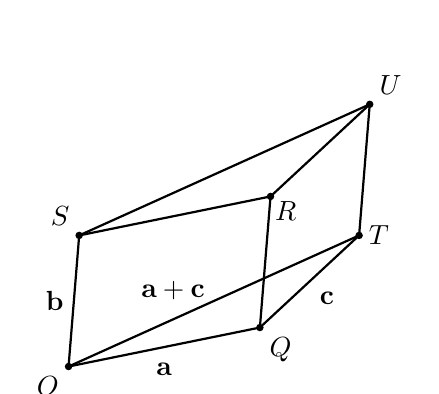
\begin{tikzpicture}[>=Stealth, scale=0.9, line cap=round, line join=round]
    \coordinate (O) at (0,0);
    \coordinate (Q) at (2.7, 0.55);
    \coordinate (T) at (4.1, 1.85);
    \coordinate (S) at (0.15, 1.85);
    \coordinate (R) at ($(Q)+(S)$);
    \coordinate (U) at ($(T)+(S)$);

    \draw[thick] (O) -- (Q) node[midway, below=2pt] {$\vect{a}$};
    \draw[thick] (Q) -- (T) node[midway, below right] {$\vect{c}$};
    \draw[thick] (O) -- (S) node[midway, left] {$\vect{b}$};
    \draw[thick] (S) -- (R) -- (U);
    \draw[thick] (Q) -- (R);
    \draw[thick] (T) -- (U);
    \draw[thick] (O) -- (T);
    \node[above left, inner sep=1pt] at ($(O)!0.48!(T)$) {$\vect{a}+\vect{c}$};
    \draw[thick] (S) -- (U);

    \fill (O) circle (1.5pt) node[below left] {$O$};
    \fill (Q) circle (1.5pt) node[below right] {$Q$};
    \fill (T) circle (1.5pt) node[right] {$T$};
    \fill (S) circle (1.5pt) node[above left] {$S$};
    \fill (R) circle (1.5pt) node[below right, inner sep=1.5pt] {$R$};
    \fill (U) circle (1.5pt) node[above right] {$U$};
  \end{tikzpicture}
  \caption*{圖 2-5}\label{fig:b6s-2-5}
  \end{figure}

  \item $V(\vect{a}, \vect{b}+\lambda\vect{a}) = V(\vect{a}, \vect{b})$\\
  如圖 2-6，同底等高的平行四邊形面積相同。同理 $V(\vect{a}+\lambda\vect{b}, \vect{b}) = V(\vect{a}, \vect{b})$。

  \begin{figure}[H]
  \centering
  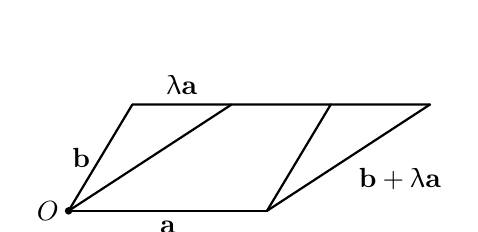
\begin{tikzpicture}[>=Stealth, scale=0.9, line cap=round, line join=round]
    \coordinate (O) at (0,0);
    \coordinate (A) at (2.8, 0);
    \coordinate (B) at (0.9, 1.5);
    \coordinate (AB) at ($(A)+(B)$);
    \coordinate (Bp) at ($(B)+(1.4, 0)$);
    \coordinate (ABp) at ($(AB)+(1.4, 0)$);

    \draw[thick] (O) -- (A) node[midway, below] {$\vect{a}$};
    \draw[thick] (O) -- (B) node[midway, left] {$\vect{b}$};
    \draw[thick] (B) -- (AB) -- (A);

    \draw[thick] (O) -- (Bp);
    \draw[thick] (A) -- (ABp) node[midway, below right] {$\vect{b}+\lambda\vect{a}$};
    \draw[thick] (AB) -- (ABp);
    \node[above] at ($(B)!0.5!(Bp)$) {$\lambda\vect{a}$};

    \fill (O) circle (1.5pt) node[left] {$O$};
  \end{tikzpicture}
  \caption*{圖 2-6}\label{fig:b6s-2-6}
  \end{figure}

  \item $V(\vect{a}, \vect{a}) = 0$\\
  因為在平面上，一線段的面積為 0。

  \item $\vect{e}_1=(1, 0), \vect{e}_2=(0, 1)$，則
  \[ V(\vect{e}_1, \vect{e}_2) = 1 \]
  因邊長為 1 的正方形其面積為 1。
\end{enumerate}

\subsubsection*{作業 18}\label{hw:b6s-1-18}
\begin{enumerate}[label=(\roman*), leftmargin=2em]
  \item 以上從 I 到 V 的性質，對 $\mathbb{R}^3$ 中平行六面體亦相應成立，試將其相應性質用式子列出。
  \item $\mathbb{R}^1$ 中又當如何去敘述？
\end{enumerate}

以上性質事實上有些可以從另一些導出，是彼此相關的。我們將抽出其中幾個，將之推廣到一般 $\mathbb{R}^n$ 中。

\begin{definition}\label{def:b6s-1-5}
設 $V$ 為 $\mathbb{R}^n$ 中自 $n$ 個向量 $\vect{a}_1, \vect{a}_2, \dots, \vect{a}_n$ 映至 $\mathbb{R}$ 的函數，記作 $V(\vect{a}_1, \vect{a}_2, \dots, \vect{a}_n)$ 滿足下列四個性質：
\begin{enumerate}[label=(\Alph*), leftmargin=2em]
  \item $V(\vect{a}_1, \dots, \vect{a}_i, \dots, \vect{a}_n) = V(\vect{a}_1, \dots, \vect{a}_i + \vect{a}_k, \dots, \vect{a}_n); \quad i \ne k, 1 \le i \le n, 1 \le k \le n$
  \item $V(\vect{a}_1, \dots, \lambda\vect{a}_i, \dots, \vect{a}_n) = \lambda V(\vect{a}_1, \dots, \vect{a}_i, \dots, \vect{a}_n) \qquad 1 \le i \le n$
  \item $V(\vect{b} + \vect{c}, \vect{a}_2, \dots, \vect{a}_n) = V(\vect{b}, \vect{a}_2, \dots, \vect{a}_n) + V(\vect{c}, \vect{a}_2, \dots, \vect{a}_n)$
  \item $V(\vect{e}_1, \vect{e}_2, \dots, \vect{e}_n) = 1$
\end{enumerate}
此函數 $V$ 稱為\textbf{行列式}（或 \textbf{$n$ 階行列式}）。
\end{definition}

亦可以把 $V$ 看作是 $\mathbb{R}^{n^2}$ 到 $\mathbb{R}$ 的函數。又若把 $\vect{a}_i$ 看作列向量，我們可以把 $V$ 看作將 $n$ 階方陣映至 $\mathbb{R}$ 的函數，常記作
\begin{equation}
V(\vect{a}_1, \vect{a}_2, \dots, \vect{a}_n) = \begin{vmatrix}
a_{11} & a_{12} & \dots & a_{1n} \\
a_{21} & a_{22} & \dots & a_{2n} \\
\dots & \dots & \dots & \dots \\
a_{n1} & a_{n2} & \dots & a_{nn}
\end{vmatrix} \label{eq:b6s-1-2-4}
\end{equation}
\begin{equation}
\text{或簡記作 } |a_{ij}|\text{。} \tag{4'} \label{eq:b6s-1-2-4p}
\end{equation}

其中 $\vect{a}_i=(a_{i1}, a_{i2}, \dots, a_{in})$ 為列向量，$i=1, 2, \dots, n$。
所以我們仍稱 $a_{ij}$ 為第 $i$ 列第 $j$ 行的原素，$\vect{a}_j^*=(a_{1j}, a_{2j}, \dots, a_{nj})$ 為行向量。事實上我們將要看到方陣的運算與行列式的運算間有密切的關係。

現在我們面臨三個重要問題：
\begin{enumerate}[label=(\roman*), leftmargin=2em]
  \item 這種行列式函數是否存在？
  \item 若是存在，是否僅有一個這樣的函數？（此即唯一性）
  \item 假設存在而且唯一，我們又如何去計算 $V(\vect{a}_1, \vect{a}_2, \dots, \vect{a}_n)$ 呢？
\end{enumerate}

\paragraph{注意：}(C) 稱作行列式加法定理，事實上可由 (A), (B) 兩式證得（參閱附錄 II）。為了簡化討論和集中注意，我們在課文內將不深究。

由上面的討論可以理解，若對 (i), (ii) 的答案均是肯定的，我們可以用行列式來定義 $n$ 維平行體的“有向體積”，因為此時滿足這些性質的函數為唯一存在。

\subsubsection*{習題 I-2}\label{sec:b6s-ex1-2}

\begin{enumerate}[label=\arabic*., leftmargin=2em]
  \item 當 $\vect{a}_1, \vect{a}_2$ 為下列各種情形時，試求 $V(\vect{a}_1, \vect{a}_2)$ 並作圖：
  \begin{enumerate}[label=(\roman*)]
    \item $\vect{a}_1=(1, 2), \vect{a}_2=(3, -1)$
    \item $\vect{a}_1=(-1, 3), \vect{a}_2=(-2, 0)$
  \end{enumerate}

  \item 當 $\vect{a}_1, \vect{a}_2, \vect{a}_3$ 為下列各種情形時，試求 $V(\vect{a}_1, \vect{a}_2, \vect{a}_3)$ 並作圖：
  \begin{enumerate}[label=(\roman*)]
    \item $\vect{a}_1=(1, 0, 1), \vect{a}_2=(0, 1, 1), \vect{a}_3=(1, 1, 0)$
    \item $\vect{a}_1=(1, -1, 2), \vect{a}_2=(-1, 0, 3), \vect{a}_3=(0, 2, -1)$
  \end{enumerate}

  \item $P=(1, -2, 1), Q=(2, 0, 2), R=(5, 6, 3)$ 試求 $\triangle PQR$ 的面積。

  \stepcounter{enumi}
  \item[\textbf{*4.}] 設 $U$ 為 $\mathbb{R}^n$ 中任何 $n$ 個向量 $\vect{a}_1, \vect{a}_2, \dots, \vect{a}_n$ 映到 $\mathbb{R}$ 的一個函數，記作 $U(\vect{a}_1, \vect{a}_2, \dots, \vect{a}_n)$ 且滿足 (A), (B), (C) 三性質。若 $k$ 為一實數，令
  \[ W(\vect{a}_1, \vect{a}_2, \dots, \vect{a}_n) = k U(\vect{a}_1, \vect{a}_2, \dots, \vect{a}_n) \]
  則是否 $W$ 也滿足 (A), (B), (C) 三性質？

  \stepcounter{enumi}
  \item[\textbf{*5.}] $\mathbb{R}^3$ 中由不共面的四點 $P, Q, R, S$ 為頂點所張成的凸面體稱為四面體，即
  \[ \text{四面體} = \{ \vec{OT} : \vec{OT} = \lambda_1\vec{OP} + \lambda_2\vec{OQ} + \lambda_3\vec{OR} + \lambda_4\vec{OS}, \lambda_1+\lambda_2+\lambda_3+\lambda_4 = 1 \} \]
  若已知四面體的體積為 $P, Q, R, S$ 所張成平行六面體體積的六分之一。試求下列各四點所成四面體的體積：
  \begin{enumerate}[label=(\roman*)]
    \item $(0, 0, 0), (1, 0, 0), (0, 1, 0), (0, 2, 3)$
    \item $(0, 1, 2), (3, 1, 4), (1, 2, 3), (4, 1, 0)$
  \end{enumerate}

  \item 設 $P, Q, R, S \in \mathbb{R}^3$，試求在下面情形時，四面體的面積，若所得面積為零時，則 $P, Q, R, S$ 之關係為何？
  \phantomsection\label{note:b6s-ch1-p30-s-coord}%
  \[ P=(1, 1, 0), Q=(0, -1, 1), R=(-4, 1, -5), S=(0, 0, 0)\footnotemark \]
  \footnotetext{【原書校訂】：原書此處印作「$S=(0,0,0($」，右括弧印損，茲校訂補正為「$S=(0,0,0)$」。}

  \item 設 $\vect{a}_1=(a_{11}, a_{12}, a_{13}), \vect{a}_2=(a_{21}, a_{22}, a_{23})$ 為 $\mathbb{R}^3$ 中二向量，試證 $\vect{a}_1, \vect{a}_2$ 所張平行四邊形的面積為
  \[ \sqrt{\begin{vmatrix} a_{12} & a_{13} \\ a_{22} & a_{23} \end{vmatrix}^2 + \begin{vmatrix} a_{13} & a_{11} \\ a_{23} & a_{21} \end{vmatrix}^2 + \begin{vmatrix} a_{11} & a_{12} \\ a_{21} & a_{22} \end{vmatrix}^2} \]
\end{enumerate}

\subsection{重排與符號函數}\label{sec:b6s-1-3}
\resetsectcounters

\paragraph{觀察：}
\begin{equation}
\begin{vmatrix}
a_1 & a_2 & a_3 \\
b_1 & b_2 & b_3 \\
c_1 & c_2 & c_3
\end{vmatrix} = a_1 b_2 c_3 + a_3 b_1 c_2 + a_2 b_3 c_1 - a_3 b_2 c_1 - a_2 b_1 c_3 - a_1 b_3 c_2 \label{eq:b6s-1-3-1}
\end{equation}
我們發現三件事：
\begin{enumerate}[label=\arabic*., leftmargin=2em]
  \item 右邊的每一項 $a_i b_j c_k$ 其中 $i, j, k$ 均相異，這表明此項是由每一行每一列均只取一個原素相乘而得。
  \item 每一項 $a_i b_j c_k$ 中 $a, b, c$ 三英文字母均不同，因此可把 $a_i b_j c_k$ 與 $1, 2, 3$ 的排列作一對應，此對應顯然成一個一一對應即右邊恰有 $3!$ 項。
  \item 右邊有些項取正號，有些項取負號，這符號規則為何？又若是推廣到一般 $n$ 階情形，其符號規定有沒有一定的法則可尋？
\end{enumerate}

設 $N(n) = \{ 1, 2, \dots, n \}$，今考慮一個從 $N(n)$ 映成到 $N(n)$ 的函數 $\pi$，顯然 $\pi$ 必為一個單射。將 $\pi(1), \pi(2), \dots, \pi(n)$ 按序寫出，可看出 $\pi$ 等於是自 1 到 $n$ 這 $n$ 個正整數的一種排列。反之，任何一個這樣的排列都可以看成為自 $N(n)$ 映成到 $N(n)$ 的函數。我們有時將 $\pi$ 記為
\begin{equation}
\pi : \begin{pmatrix} 1 & 2 & \dots & n \\ \pi(1) & \pi(2) & \dots & \pi(n) \end{pmatrix} \label{eq:b6s-1-3-2}
\end{equation}
或簡寫為
\begin{equation}
(\pi(1) \, \pi(2) \, \dots \, \pi(n)) \tag{2'} \label{eq:b6s-1-3-2p}
\end{equation}

\begin{example}\label{ex:b6s-1-12}
設 $\pi: N(5) \longrightarrow N(5)$ 定義如下：
\[ \pi : \begin{pmatrix} 1 & 2 & 3 & 4 & 5 \\ \pi(1) & \pi(2) & \pi(3) & \pi(4) & \pi(5) \end{pmatrix} \]
$\pi(1)=3, \pi(2)=5, \pi(3)=4, \pi(4)=1, \pi(5)=2$。
若寫作 $(3 \; 5 \; 4 \; 1 \; 2)$ 就更清楚看出 $\pi$ 代表一種 $N(5)$ 的排列。\hfill$\#$
\end{example}

\begin{definition}\label{def:b6s-1-6}
一個自 $N(n)$ 映成到 $N(n)$ 的函數 $\pi$ 稱作一個\textbf{重排}。
\end{definition}

在上例中有些數字的大小次序保持不變，有些卻更改了。例如 3 4 和 1 2 次序保持不變，可是 5 4 和 3 1 等次序卻改變了。在 $\pi$ 之下若有一對 $i, j, i < j$，使得 $\pi(i) > \pi(j)$，則稱重排 $\pi$ 有一個\textbf{倒置}。$\pi$ 中所有倒置的個數稱為\textbf{倒置數}，記為 $\#\pi$，或作 $\#(\pi(1)\pi(2)\dots\pi(n))$。

\begin{example}\label{ex:b6s-1-13}
$\pi$ 如例 1，$\pi$ 的倒置數為何？
\end{example}

\paragraph{【解】}
$\pi$ 中所有倒置如下：$31, 32, 54, 51, 52, 41, 42$ 所以 $\#\pi = 7$。\hfill$\#$

關於倒置數，可看作將 $(\pi(1)\pi(2)\dots\pi(n))$ 的次序排回 $(1 \; 2 \; \dots \; n)$ 的次序所需經過對調兩數字的總次數。

\begin{example}\label{ex:b6s-1-14}
$\pi$ 如例 2 表為 $(3 \; 5 \; 4 \; 1 \; 2)$，首先將 1 與 4 對調得 $(3 \; 5 \; 1 \; 4 \; 2)$，第二次將 1 與 5 對調得 $(3 \; 1 \; 5 \; 4 \; 2)$，第三次將 1 與 3 對調得 $(1 \; 3 \; 5 \; 4 \; 2)$，第四次將 2 與 5 對調得 $(1 \; 3 \; 2 \; 4 \; 5)$，第五次將 2 與 5 對調得 $(1 \; 3 \; 2 \; 5 \; 4)$，第六次將 2 與 3 對調得 $(1 \; 2 \; 3 \; 5 \; 4)$，第七次將 5 與 4 對調得 $(1 \; 2 \; 3 \; 4 \; 5)$。\hfill$\#$
\end{example}

\paragraph{注意：}我們也可以首先將 5 與 4 對調，其次將 1 與 5 對調等等。最後當我們比較兩次不同的過程，就會發現比如 5 與 1 的對調在兩次過程中出現的次序容或有不同，但卻相同的都出現一次。即所有的對調數並不因採行的過程不同而有所影響。

關於對調數還有一個實用之法來計算。今以前例作為說明。

\begin{discussion}\label{disc:b6s-1-2}
$\pi$ 如前例，試求其倒置數。
\end{discussion}

\paragraph{【解】}
首先將 $\pi$ 如下寫出：
\[ \begin{matrix} 1 & 2 & 3 & 4 & 5 \\ 3 & 5 & 4 & 1 & 2 \end{matrix} \]

其次將表中上列與下列中相同的數字以直線相連，但要注意在劃線時不要讓三線以上有共點的情形發生：

\begin{figure}[H]
\centering
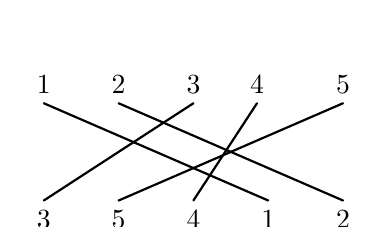
\begin{tikzpicture}[scale=0.95, line cap=round, line join=round]
  % Top row (slightly nudge 5 to avoid any triple intersection)
  \node (t1) at (1.0, 1.8) {$1$};
  \node (t2) at (2.0, 1.8) {$2$};
  \node (t3) at (3.0, 1.8) {$3$};
  \node (t4) at (3.85, 1.8) {$4$};
  \node (t5) at (5.0, 1.8) {$5$};
  % Bottom row
  \node (b3) at (1.0, 0) {$3$};
  \node (b5) at (2.0, 0) {$5$};
  \node (b4) at (3.0, 0) {$4$};
  \node (b1) at (4.0, 0) {$1$};
  \node (b2) at (5.0, 0) {$2$};
  % Connecting lines: 7 distinct pairwise intersections
  \draw[thick] (t1.south) -- (b1.north);
  \draw[thick] (t2.south) -- (b2.north);
  \draw[thick] (t3.south) -- (b3.north);
  \draw[thick] (t4.south) -- (b4.north);
  \draw[thick] (t5.south) -- (b5.north);
\end{tikzpicture}
\end{figure}

最後計算交點的個數正好是 7。現在來分析一下緣由：今以 1, 3 兩對數字所相應一對斜直線的交點為例，二斜直線所以會相交表明 1 3 在 $\pi$ 之下有了倒置，所以必相應一個對調。有 7 個交點表明有 7 個對調，所以倒置數為 7\footnote{\begin{minipage}[t]{0.95\linewidth}【原書註】：在計算符號函數時若有如下交點時：\par\smallskip
\centering
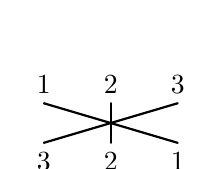
\begin{tikzpicture}[scale=0.85, line cap=round, line join=round]
  \node (u1) at (1, 1.15) {$1$}; \node (u2) at (2, 1.15) {$2$}; \node (u3) at (3, 1.15) {$3$};
  \node (d3) at (1, 0) {$3$}; \node (d2) at (2, 0) {$2$}; \node (d1) at (3, 0) {$1$};
  \draw[thick] (u1.south) -- (d1.north);
  \draw[thick] (u2.south) -- (d2.north);
  \draw[thick] (u3.south) -- (d3.north);
\end{tikzpicture}\par\smallskip
\raggedright 垂直線與斜線的交點可以不計。因垂直線與它線交點的總數必為偶數，不影響正負號。
\end{minipage}}。

下面的定義也是行列式展開式中的每一項其正負號的來源。

\begin{definition}\label{def:b6s-1-7}
設 $F = \{ \pi : \pi \text{ 為 } N(n) \text{ 的重排} \}$（$F$ 共有 $n!$ 個元素），下面函數稱作\textbf{符號函數}，以 $\operatorname{sgn}$ 表示：
\[ \operatorname{sgn}(\pi) = \begin{cases}
1, & \#\pi \text{ 為偶數} \\
-1, & \#\pi \text{ 為奇數}
\end{cases} \]
通常 $\operatorname{sgn}(\pi)$ 亦可記為 $\operatorname{sgn}(\pi(1)\pi(2)\dots\pi(n))$。一般約定若 $\pi$ 不是映射，則定 $\operatorname{sgn}(\pi) = 0$。
\end{definition}

\subsubsection*{作業 19}\label{hw:b6s-1-19}
試由上面定義中找到 (1) 式各項正負號的規則。

\subsubsection*{習題 I-3}\label{sec:b6s-ex1-3}

\begin{enumerate}[label=\arabic*., leftmargin=2em]
  \item 設 $\pi$ 為下列各種情形時，試求 $\pi$ 的倒置數及 $\operatorname{sgn}(\pi)$：
  \begin{enumerate}[label=(\roman*)]
    \item $\pi = \begin{pmatrix} 1 & 2 & 3 & 4 & 5 \\ 2 & 3 & 4 & 5 & 1 \end{pmatrix}$
    \item $\pi = (3 \; 2 \; 4 \; 1 \; 6 \; 5)$
    \item $\pi = (7 \; 6 \; 5 \; 4 \; 3 \; 2 \; 1)$
  \end{enumerate}

  \stepcounter{enumi}
  \item[\textbf{*2.}] 設 $\pi \circ \pi^*$ 皆為 $N(n)$ 的重排
  \begin{enumerate}[label=(\roman*)]
    \item 試證合成函數 $\pi \circ \pi^*$ 也是 $N(n)$ 的一個重排。
    \item 試問 $\operatorname{sgn}(\pi \circ \pi^*)$ 與 $\operatorname{sgn}(\pi), \operatorname{sgn}(\pi^*)$ 之間的關係為何？
  \end{enumerate}

  \stepcounter{enumi}
  \item[\textbf{*3.}] 設 $i, j$ 為正整數，$1 \le i \le j \le n$，令
  \[ \pi_{ij} = \begin{pmatrix}
  1 & 2 & \dots & i-1 & i & i+1 & \dots & j-1 & j & j+1 & \dots & n \\
  1 & 2 & \dots & i-1 & j & i+1 & \dots & j-1 & i & j+1 & \dots & n
  \end{pmatrix} \]
  即將 $i, j$ 互調，其他數不動，試求 $\#\pi_{ij}$ 及 $\operatorname{sgn}(\pi_{ij})$。（提示：當 $n=4, 5$ 時，嚐試先作）

  \item 設 $\pi = (7 \; 6 \; 5 \; 4 \; 3 \; 2 \; 1)$。
  \begin{enumerate}[label=(\roman*)]
    \item 試證 $\pi = \pi_{17} \cdot \pi_{26} \cdot \pi_{35}$。
    \item 由習題 2, 3 試求 $\operatorname{sgn}(\pi)$ 之值。
  \end{enumerate}
\end{enumerate}

\subsection{行列式的基本性質}\label{sec:b6s-1-4}
\resetsectcounters

在討論滿足 (A), (B), (C), (D) 的行列式函數是否存在以前，讓我們先從 (A), (B), (C), (D) 諸式推演行列式的若干性質：

\begin{theorem}\label{thm:b6s-1-2}
$V(\vect{a}_1, \dots, \vect{a}_i, \dots, \vect{a}_n) = V(\vect{a}_1, \dots, \vect{a}_i + \lambda\vect{a}_k, \vect{a}_{i+1}, \dots, \vect{a}_n)$ 其中 $i \ne k$，$\lambda$ 為任意實數。亦即將 $\vect{a}_i$ 易為 $\vect{a}_i + \lambda\vect{a}_k$ 行列式的值不變。
\end{theorem}

\begin{proof}[【證明】]
$\lambda=0$ 時顯然成立。今假定 $\lambda \ne 0$，由 (B) 得
\[ V(\vect{a}_1, \dots, \lambda\vect{a}_k, \vect{a}_{k+1}, \dots, \vect{a}_n) = \lambda V(\vect{a}_1, \dots, \vect{a}_k, \vect{a}_{k+1}, \dots, \vect{a}_n) \]
又根據 (A)
\begin{align*}
V(\vect{a}_1, \dots, \vect{a}_i + \lambda\vect{a}_k, \dots, \lambda\vect{a}_k, \dots, \vect{a}_n) &= V(\vect{a}_1, \dots, \vect{a}_i, \dots, \lambda\vect{a}_k, \dots, \vect{a}_n) \\
&= \lambda V(\vect{a}_1, \dots, \vect{a}_i, \dots, \vect{a}_k, \dots, \vect{a}_n)
\end{align*}
（此處雖寫成 $i < k$ 的情形，其實對 $k < i$ 也是一樣的）\\
所以
\begin{align*}
\dfrac{1}{\lambda} V(\vect{a}_1, \dots, \vect{a}_i + \lambda\vect{a}_k, \dots, \lambda\vect{a}_k, \dots, \vect{a}_n) &= V(\vect{a}_1, \dots, \vect{a}_i, \dots, \vect{a}_k, \dots, \vect{a}_n)
\end{align*}
即
\[ V(\vect{a}_1, \dots, \vect{a}_i + \lambda\vect{a}_k, \dots, \vect{a}_k, \dots, \vect{a}_n) = V(\vect{a}_1, \dots, \vect{a}_i, \dots, \vect{a}_k, \dots, \vect{a}_n) \]
\end{proof}\hfill$\#$

下面的定理讀者試自證之：

\begin{theorem}\label{thm:b6s-1-3}
$V(\vect{a}_1, \dots, \vect{a}_i, \dots, \vect{a}_n) = V\left(\vect{a}_1, \dots, \vect{a}_i + \sum_{\substack{k=1\\ k\ne i}}^n \lambda_k \vect{a}_k, \vect{a}_{i+1}, \dots, \vect{a}_n\right)$。
\end{theorem}

\begin{theorem}\label{thm:b6s-1-4}
$\vect{a}_1, \vect{a}_2, \dots, \vect{a}_n$ 中若有一為零向量，則
\[ V(\vect{a}_1, \vect{a}_2, \dots, \vect{a}_n) = 0 \]
\end{theorem}

\begin{proof}[【證明】]
設 $\vect{a}_i = \vect{0}$ 則 $\vect{a}_i = 0\vect{a}_i$ 所以
\begin{align*}
V(\vect{a}_1, \dots, \vect{a}_i, \dots, \vect{a}_n) &= V(\vect{a}_1, \dots, 0\vect{a}_i, \dots, \vect{a}_n) \\
&= 0 V(\vect{a}_1, \dots, \vect{a}_i, \dots, \vect{a}_n) = 0
\end{align*}
\end{proof}\hfill$\#$

\begin{theorem}\label{thm:b6s-1-5}
若 $\vect{a}_1, \vect{a}_2, \dots, \vect{a}_n$ 線性相關，則 $V(\vect{a}_1, \vect{a}_2, \dots, \vect{a}_n) = 0$。
\end{theorem}

\begin{proof}[【證明】]
由條件知 $\vect{a}_1, \vect{a}_2, \dots, \vect{a}_n$ 中必有一向量為其餘諸向量的線性組合，設
\begin{equation}
\vect{a}_i = \sum_{\substack{k=1\\ k\ne i}}^n \lambda_k \vect{a}_k \label{eq:b6s-1-4-1}
\end{equation}
根據定理 2 將 $\vect{a}_i$ 易作 $\vect{a}_i + \sum_{\substack{k=1\\ k\ne i}}^n (-\lambda_k)\vect{a}_k$，行列式的值不變。所以
\begin{align*}
V(\vect{a}_1, \dots, \vect{a}_i, \dots, \vect{a}_n) &= V\left(\vect{a}_1, \dots, \vect{a}_i + \sum_{\substack{k=1\\ k\ne i}}^n (-\lambda_k)\vect{a}_k, \dots, \vect{a}_n\right) \\
&= V(\vect{a}_1, \dots, \vect{0}, \vect{a}_{i+1}, \dots, \vect{a}_n) = 0
\end{align*}
\end{proof}\hfill$\#$

\begin{corollary}\label{cor:b6s-1-1}
若 $\vect{a}_1, \vect{a}_2, \dots, \vect{a}_n$ 中有二向量相等或平行，則 $V(\vect{a}_1, \vect{a}_2, \dots, \vect{a}_n) = 0$。
\end{corollary}

\begin{theorem}\label{thm:b6s-1-6}
若將 $\vect{a}_1, \vect{a}_2, \dots, \vect{a}_n$ 中任意二向量互換，則行列式變號，亦即：
\[ V(\vect{a}_1, \dots, \vect{a}_i, \dots, \vect{a}_k, \dots, \vect{a}_n) = -V(\vect{a}_1, \dots, \vect{a}_k, \dots, \vect{a}_i, \dots, \vect{a}_n) \]
\end{theorem}

\begin{proof}[【證明】]
多次應用 (A) 可得
\begin{align*}
&V(\vect{a}_1, \dots, \vect{a}_i, \dots, \vect{a}_k, \dots, \vect{a}_n) \\
&= V(\vect{a}_1, \dots, \vect{a}_i + \vect{a}_k, \dots, \vect{a}_k, \dots, \vect{a}_n) \\
&= V(\vect{a}_1, \dots, \vect{a}_i + \vect{a}_k, \dots, \vect{a}_k - (\vect{a}_i + \vect{a}_k), \dots, \vect{a}_n) \\
&= V(\vect{a}_1, \dots, \vect{a}_i + \vect{a}_k, \dots, -\vect{a}_i, \vect{a}_{k+1}, \dots, \vect{a}_n) \\
&= V(\vect{a}_1, \dots, (\vect{a}_i + \vect{a}_k) - \vect{a}_i, \vect{a}_{i+1}, \dots, -\vect{a}_i, \vect{a}_{k+1}, \dots, \vect{a}_n) \\
&= V(\vect{a}_1, \dots, \vect{a}_k, \vect{a}_{i+1}, \dots, -\vect{a}_i, \vect{a}_{k+1}, \dots, \vect{a}_n) \\
\text{由 (B)} \\
&= -V(\vect{a}_1, \dots, \vect{a}_k, \vect{a}_{i+1}, \dots, \vect{a}_i, \vect{a}_{k+1}, \dots, \vect{a}_n)
\end{align*}
\end{proof}\hfill$\#$

\begin{example}\label{ex:b6s-1-15}
$\begin{vmatrix} 1 & 2 & 3 \\ 3 & 1 & 2 \\ 2 & 3 & 1 \end{vmatrix} \overset{\text{由定理 1}}{=} \begin{vmatrix} 1+3 & 2+1 & 3+2 \\ 3 & 1 & 2 \\ 2 & 3 & 1 \end{vmatrix} = 18$。\hfill$\#$
\end{example}

\begin{example}\label{ex:b6s-1-16}
$\begin{vmatrix} 1 & 2 & 3 \\ 3 & 1 & 2 \\ 2 & 3 & 1 \end{vmatrix} = - \begin{vmatrix} 3 & 1 & 2 \\ 1 & 2 & 3 \\ 2 & 3 & 1 \end{vmatrix}$ （由定理 5）。\hfill$\#$
\end{example}

\begin{example}\label{ex:b6s-1-17}
$\begin{vmatrix} 0 & 0 & 0 \\ 1 & 2 & 3 \\ x & y & z \end{vmatrix} = 0$ （系理 1）。\hfill$\#$
\end{example}

\begin{example}\label{ex:b6s-1-18}
求 $x$ 的值使
\[ \begin{vmatrix} 1 & 1 & 1 \\ 3 & 2 & 4 \\ x & 1 & 2 \end{vmatrix} = 0 \]
\end{example}

\paragraph{【解】}
$x = \dfrac{3}{2}$ 當時二、三列向量平行，故此時行列式的值為 0，又知原式必為一關於 $x$ 的一個一次方程故僅有一解。\hfill$\#$

\subsubsection*{作業 20}\label{hw:b6s-1-20}
試比較 $\begin{vmatrix} a_1 & a_2 & a_3 \\ b_1 & b_2 & b_3 \\ c_1 & c_2 & c_3 \end{vmatrix}$ 與 $\begin{vmatrix} c_1 & c_2 & c_3 \\ b_1 & b_2 & b_3 \\ a_1 & a_2 & a_3 \end{vmatrix}$。

\subsubsection*{作業 21}\label{hw:b6s-1-21}
計算 $\begin{vmatrix} a & a & a \\ x & y & z \\ 1 & 1 & 1 \end{vmatrix}$。

\begin{theorem}\label{thm:b6s-1-7}
設 $\vect{a}_i = \sum_{j=1}^r \vect{b}_i^j, \quad i=1, 2, \dots, n$
則
\[ V(\vect{a}_1, \vect{a}_2, \dots, \vect{a}_n) = \sum_{v_1, v_2, \dots, v_n=1}^r V(\vect{b}_1^{v_1}, \vect{b}_2^{v_2}, \dots, \vect{b}_n^{v_n}) \]
（$\sum_{v_1, v_2, \dots, v_n=1}^r \equiv \sum_{v_1=1}^r \sum_{v_2=1}^r \dots \sum_{v_n=1}^r$）
\end{theorem}

\begin{proof}[【證明】]
首先由 (C) 得到
\[ V(\vect{a}_1, \vect{a}_2, \dots, \vect{a}_n) = \sum_{v_1=1}^r V(\vect{b}_1^{v_1}, \vect{a}_2, \dots, \vect{a}_n) \]
根據定理 5
\begin{align*}
\sum_{v_1=1}^r V\left(\vect{b}_1^{v_1}, \sum_{v_2=1}^r \vect{b}_2^{v_2}, \vect{a}_3, \dots, \vect{a}_n\right) &= - \sum_{v_1=1}^r V\left(\sum_{v_2=1}^r \vect{b}_2^{v_2}, \vect{b}_1^{v_1}, \vect{a}_3, \dots, \vect{a}_n\right) \\
&= - \sum_{v_1=1}^r \sum_{v_2=1}^r V(\vect{b}_2^{v_2}, \vect{b}_1^{v_1}, \vect{a}_3, \dots, \vect{a}_n) \\
&= \sum_{v_1=1}^r \sum_{v_2=1}^r V(\vect{b}_1^{v_1}, \vect{b}_2^{v_2}, \vect{a}_3, \dots, \vect{a}_n) = \dots \\
&= \sum_{v_1=1}^r \sum_{v_2=1}^r \dots \sum_{v_n=1}^r V(\vect{b}_1^{v_1}, \vect{b}_2^{v_2}, \dots, \vect{b}_n^{v_n}) \\
&= \sum_{v_1, v_2, \dots, v_n=1}^r V(\vect{b}_1^{v_1}, \vect{b}_2^{v_2}, \dots, \vect{b}_n^{v_n})
\end{align*}
\end{proof}\hfill$\#$

\begin{theorem}\label{thm:b6s-1-8}
設 $\vect{b}_1, \vect{b}_2, \dots, \vect{b}_n$ 線性無關，而 $V(\vect{b}_1, \vect{b}_2, \dots, \vect{b}_n) = 0$，則對任何 $\vect{a}_1, \vect{a}_2, \dots, \vect{a}_n$ 均有 $V(\vect{a}_1, \vect{a}_2, \dots, \vect{a}_n) = 0$。
\end{theorem}

\begin{proof}[【證明】]
根據 § I-1 丙的 I 知任 $\vect{a}_1, \vect{a}_2, \dots, \vect{a}_n$ 皆可表為這些 $\vect{b}_i$ 的線性組合
\begin{equation}
\vect{a}_i = \sum_{k=1}^n \lambda_{ik} \vect{b}_k \qquad i=1, 2, \dots, n \label{eq:b6s-1-4-2}
\end{equation}
則
\begin{align*}
V(\vect{a}_1, \vect{a}_2, \dots, \vect{a}_n) &= V\left(\sum_{v_1=1}^n \lambda_{1v_1} \vect{b}_{v_1}, \dots, \sum_{v_n=1}^n \lambda_{nv_n} \vect{b}_{v_n}\right) \\
&= \sum_{v_1, \dots, v_n=1}^n V(\lambda_{1v_1} \vect{b}_{v_1}, \lambda_{2v_2} \vect{b}_{v_2}, \dots, \lambda_{nv_n} \vect{b}_{v_n}) \\
&= \sum_{v_1, \dots, v_n=1}^n \lambda_{1v_1} \lambda_{2v_2} \dots \lambda_{nv_n} V(\vect{b}_{v_1}, \vect{b}_{v_2}, \dots, \vect{b}_{v_n})
\end{align*}
其中 $V(\vect{b}_{v_1}, \vect{b}_{v_2}, \dots, \vect{b}_{v_n})$ 有兩種可能：
\begin{enumerate}[label=(\roman*), leftmargin=2em]
  \item 有二指標 $v_i = v_j$ ($i \ne j$) 此時 $V(\vect{b}_{v_1}, \vect{b}_{v_2}, \dots, \vect{b}_{v_n}) = 0$（系理 1）。
  \item 諸指標 $v_i$ 皆相異，由假設及定理 5
  \[ |V(\vect{b}_{v_1}, \vect{b}_{v_2}, \dots, \vect{b}_{v_n})| = |V(\vect{b}_1, \vect{b}_2, \dots, \vect{b}_n)| = 0 \]
\end{enumerate}
所以定理得證。\end{proof}\hfill$\#$

\begin{theorem}\label{thm:b6s-1-9}
$V(\vect{a}_1, \vect{a}_2, \dots, \vect{a}_n) \ne 0$ 為 $\vect{a}_1, \vect{a}_2, \dots, \vect{a}_n$ 線性無關之充要條件。
\end{theorem}

\begin{proof}[【證明】]
\begin{enumerate}[label=(\arabic*), leftmargin=2em]
  \item 若 $\vect{a}_1, \vect{a}_2, \dots, \vect{a}_n$ 線性無關且 $V(\vect{a}_1, \vect{a}_2, \dots, \vect{a}_n) = 0$，則根據定理 7，$V \equiv 0$。但 $V(\vect{e}_1, \vect{e}_2, \dots, \vect{e}_n) = 1$，所以 $V(\vect{a}_1, \vect{a}_2, \dots, \vect{a}_n) \ne 0$。
  \item 若 $\vect{a}_1, \vect{a}_2, \dots, \vect{a}_n$ 線性相關，適當安排指標可以假設
  \[ \vect{a}_1 = \sum_{i=2}^n \lambda_i \vect{a}_i \qquad (\lambda_i \text{ 為實數}) \]
  則
  \begin{align*}
  V(\vect{a}_1, \vect{a}_2, \dots, \vect{a}_n) &= V\left(\sum_{i=2}^n \lambda_i \vect{a}_i, \vect{a}_2, \dots, \vect{a}_n\right) \\
  &= \sum_{i=2}^n \lambda_i V(\vect{a}_i, \vect{a}_2, \dots, \vect{a}_n) = 0
  \end{align*}
\end{enumerate}
\end{proof}\hfill$\#$

\paragraph{注意：}在定理 8 之前，(D) 式沒有用到。

\begin{example}\label{ex:b6s-1-19}
試問 $(1, 2, 3), (3, 1, 2), (2, 3, 1)$ 為線性相關抑為線性無關？
\end{example}

\paragraph{【解】}
因為 $\begin{vmatrix} 1 & 2 & 3 \\ 3 & 1 & 2 \\ 2 & 3 & 1 \end{vmatrix} = 18 \ne 0$，故由定理 8 為線性無關。\hfill$\#$

\begin{example}\label{ex:b6s-1-20}
試問 $(1, 1, 1), (3, 2, 4), (x, 1, 2)$ 當 $x$ 為何值時線性無關，又為何值時線性相關？
\end{example}

\paragraph{【解】}
由例 4 的討論知 $\begin{vmatrix} 1 & 1 & 1 \\ 3 & 2 & 4 \\ x & 1 & 2 \end{vmatrix} = 0 \iff x = \dfrac{3}{2}$。
故當 $x = \dfrac{3}{2}$ 時三向量線性相關；$x \ne \dfrac{3}{2}$ 時三向量線性無關。\hfill$\#$

\begin{example}\label{ex:b6s-1-21}
試證
\[ \begin{vmatrix}
a-b & b-c & c-a \\
2 & -1 & -1 \\
b+c-2a & c+a-2b & a+b-2c
\end{vmatrix} = 0 \]
\end{example}

\begin{proof}[【證明】]
（由 (A)）
\begin{align*}
\begin{vmatrix}
a-b & 2 & b+c-2a \\
b-c & -1 & c+a-2b \\
c-a & -1 & a+b-2c
\end{vmatrix}
&= \begin{vmatrix}
0 & 0 & 0 \\
b-c & -1 & c+a-2b \\
c-a & -1 & a+b-2c
\end{vmatrix} = 0
\end{align*}
\end{proof}\hfill$\#$

\subsubsection*{習題 I-4}\label{sec:b6s-ex1-4}

\begin{enumerate}[label=\arabic*., leftmargin=2em]
  \item 試證下列行列式的值為 0：
  \begin{multicols}{2}
  \begin{enumerate}[label=(\roman*)]
    \item $\begin{vmatrix} 5 & 4 & 1 \\ 3 & 2 & 1 \\ 2 & 1 & 1 \end{vmatrix}$
    \item $\begin{vmatrix} 1 & \omega & \omega^2 \\ \omega & \omega^2 & 1 \\ \omega^2 & 1 & \omega \end{vmatrix} \quad (\omega^3=1, \omega\ne 1)$
    \item $\begin{vmatrix} 7 & 13 & 4 & 6 \\ 5 & 9 & 3 & 4 \\ 8 & 12 & 4 & 7 \\ 4 & 10 & 3 & 3 \end{vmatrix}$
    \item $\begin{vmatrix}
    0 & a & b & c & d \\
    -a & 0 & e & f & g \\
    -b & -e & 0 & h & j \\
    -c & -f & -h & 0 & k \\
    -d & -g & -j & -k & 0
    \end{vmatrix}$
  \end{enumerate}
  \end{multicols}

  \item 試求下列行列式的值：
  \begin{enumerate}[label=(\roman*)]
    \item $\begin{vmatrix} 1 & 1 & 1 \\ a & b & c \\ b+c & c+a & a+b \end{vmatrix}$
    \item $\begin{vmatrix} a+2b & a+3b & a+4b \\ a+4b & a+5b & a+6b \\ a+6b & a+7b & a+8b \end{vmatrix}$
    \item $\begin{vmatrix} b+c & c+a & a+b \\ bc & ca & ab \\ b^2 c^2 & c^2 a^2 & a^2 b^2 \end{vmatrix}$
    \item $\begin{vmatrix}
    1 & 1 & 1 & 1 \\
    a & b & c & d \\
    a^2 & b^2 & c^2 & d^2 \\
    a^3+bcd & b^3+cda & c^3+dab & d^3+abc
    \end{vmatrix}$
  \end{enumerate}

  \item 試證下列各組向量為線性相關：
  \begin{enumerate}[label=(\roman*)]
    \item $(1, 3, 5), (1, 1, -1), (7, 13, 11)$
    \item $(1, 15, 14, 4), (12, 6, 7, 9), (8, 10, 11, 5), (13, 3, 2, 6)$
  \end{enumerate}

  \item 試證
  \[ \begin{vmatrix}
  b+c & c+a & a+b \\
  b'+c' & c'+a' & a'+b' \\
  b''+c'' & c''+a'' & a''+b''
  \end{vmatrix} = 2 \begin{vmatrix}
  a & b & c \\
  a' & b' & c' \\
  a'' & b'' & c''
  \end{vmatrix} \]

  \item 試求下列各式之值：
  \begin{enumerate}[label=(\roman*)]
    \item $V(\vect{e}_1+\vect{e}_2, \vect{e}_2+\vect{e}_3, \vect{e}_3+\vect{e}_4, \vect{e}_2)$
    \item $V(\vect{e}_1, \vect{e}_1+\vect{e}_2, \vect{e}_1+\vect{e}_2+\vect{e}_3, \vect{e}_1+\vect{e}_2+\vect{e}_3+\vect{e}_4, \vect{e}_1+\vect{e}_2+\vect{e}_3+\vect{e}_4+\vect{e}_5)$
    \item $\begin{vmatrix}
    0 & 1 & 0 & 0 \\
    0 & 0 & 0 & 1 \\
    0 & 0 & 1 & 0 \\
    1 & 0 & 0 & 0
    \end{vmatrix}$
    \item $\begin{vmatrix}
    0 & 0 & 2 & 1 \\
    0 & 1 & 0 & 0 \\
    -1 & 2 & 0 & 0 \\
    0 & 1 & 1 & 0
    \end{vmatrix}$
  \end{enumerate}

  \item 若 $\begin{vmatrix} x & y & z \\ 3 & 0 & 2 \\ 1 & 1 & 1 \end{vmatrix} = 1$，試求 $\begin{vmatrix} 2x & 2y & 2z \\ \frac{3}{2} & 0 & 1 \\ 1 & 1 & 1 \end{vmatrix}$。

  \item 證明 $\begin{vmatrix} 1 & a & a^2 \\ 1 & b & b^2 \\ 1 & c & c^2 \end{vmatrix} = (b-a)(c-a)(c-b)$。

  \item 求 $\begin{vmatrix}
  1 & 1 & 1 & 1 & 1 \\
  1 & 1 & 1 & -1 & -1 \\
  1 & 1 & -1 & -1 & 1 \\
  1 & -1 & -1 & 1 & 1 \\
  1 & -1 & -1 & 1 & -1
  \end{vmatrix}$。

  \stepcounter{enumi}
  \item[\textbf{*9.}] 試證 $|k a_{ij}| = k^n |a_{ij}|$。

  \item 試求下列各三向量為線性相關的充要條件：
  \begin{enumerate}[label=(\roman*)]
    \item $(3, -1, 2), (x, 1, x), (1, 2, 2)$
    \item $(3, -1, 2), (2, 1, x), (1, 2, 2)$
    \item $(1, 0, 1), (x, 0, x), (1, 2, 2)$
  \end{enumerate}
\end{enumerate}

\subsection{行列式的存在和唯一性}\label{sec:b6s-1-5}
\resetsectcounters

本節在證明行列式函數唯一存在。

\begin{theorem}\label{thm:b6s-1-10}
能滿足 (A), (B), (D) 的函數，至多僅有一個。（所以能滿足 (A), (B), (C), (D) 的函數至多僅有一個）。
\end{theorem}

\begin{proof}[【證明】]
假設存在兩個函數 $V, V^*$ 均滿足 (A), (B), (D)，令
\[ D(\vect{a}_1, \vect{a}_2, \dots, \vect{a}_n) \equiv V(\vect{a}_1, \vect{a}_2, \dots, \vect{a}_n) - V^*(\vect{a}_1, \vect{a}_2, \dots, \vect{a}_n) \]
$D$ 亦為 $\vect{a}_1, \vect{a}_2, \dots, \vect{a}_n$ 的函數。顯然，$D$ 亦滿足 (A), (B)。又
\[ D(\vect{e}_1, \vect{e}_2, \dots, \vect{e}_n) = 0 \]
根據 § I-4 定理 7，$D \equiv 0$，即 $V = V^*$。
\end{proof}\hfill$\#$

今討論行列式函數的存在性，或者換一個角度來看，我們討論它確實的形態，也就是討論行列式的完全展開式。在 § I-2，(4) 式中 $\vect{a}_i=(a_{i1}, a_{i2}, \dots, a_{in})$ 可表為
\begin{equation}
\vect{a}_i = \sum_{j=1}^n a_{ij} \vect{e}_j \qquad i=1, 2, \dots, n \label{eq:b6s-1-5-1}
\end{equation}
根據 § I-4 定理 6
\begin{align}
V(\vect{a}_1, \vect{a}_2, \dots, \vect{a}_n) &= \sum_{v_1, v_2, \dots, v_n=1}^n V(a_{1v_1} \vect{e}_{v_1}, a_{2v_2} \vect{e}_{v_2}, \dots, a_{nv_n} \vect{e}_{v_n}) \notag \\
&= \sum_{v_1, v_2, \dots, v_n=1}^n a_{1v_1} a_{2v_2} \dots a_{nv_n} V(\vect{e}_{v_1}, \vect{e}_{v_2}, \dots, \vect{e}_{v_n}) \label{eq:b6s-1-5-2}
\end{align}
今就 $V(\vect{e}_{v_1}, \vect{e}_{v_2}, \dots, \vect{e}_{v_n})$ 討論之：
\begin{enumerate}[label=(\arabic*), leftmargin=2em]
  \item 若有 $v_i = v_j$ ($i \ne j$)，$V(\vect{e}_{v_1}, \vect{e}_{v_2}, \dots, \vect{e}_{v_n}) = 0$。
  \item 若 $v_1, v_2, \dots, v_n$ 均相異，此時 $v_1, v_2, \dots, v_n$ 可以看作為 $1, 2, \dots, n$ 的一個排列。此時在 $V(\vect{e}_{v_1}, \vect{e}_{v_2}, \dots, \vect{e}_{v_n})$ 中，若 $\vect{e}_1$ 在第 $i$ 項，將 $\vect{e}_1$ 與 $\vect{e}_{i-1}$ 互換需變號一次，再與 $\vect{e}_{i-2}$ 互換又需變號一次。由此類推，可知將 $V(\vect{e}_{v_1}, \vect{e}_{v_2}, \dots, \vect{e}_{v_n})$ 中 $\vect{e}_{v_1}, \vect{e}_{v_2}, \dots, \vect{e}_{v_n}$ 經互換重新排成 $V(\vect{e}_1, \vect{e}_2, \dots, \vect{e}_n)$ 共需互換 $\#\pi$ 次，其中 $\pi=(v_1, v_2, \dots, v_n)$。
\end{enumerate}
所以
\begin{align}
V(\vect{e}_{v_1}, \vect{e}_{v_2}, \dots, \vect{e}_{v_n}) &= \operatorname{sgn}(v_1, v_2, \dots, v_n) V(\vect{e}_1, \vect{e}_2, \dots, \vect{e}_n) \notag \\
&= \operatorname{sgn}(v_1, v_2, \dots, v_n) \label{eq:b6s-1-5-3}
\end{align}
故得
\begin{align}
V(\vect{a}_1, \vect{a}_2, \dots, \vect{a}_n) &= \begin{vmatrix}
a_{11} & a_{12} & \dots & a_{1n} \\
a_{21} & a_{22} & \dots & a_{2n} \\
\dots & \dots & \dots & \dots \\
a_{n1} & a_{n2} & \dots & a_{nn}
\end{vmatrix} \notag \\
&= \sum_{v_1, v_2, \dots, v_n=1}^n \operatorname{sgn}(v_1, v_2, \dots, v_n) a_{1v_1} a_{2v_2} \dots a_{nv_n} \label{eq:b6s-1-5-4}
\end{align}

\begin{theorem}\label{thm:b6s-1-11}
滿足 (A), (B), (C), (D) 的函數存在。
\end{theorem}

\begin{proof}[【證明】]
只需利用 (4) 式證明 $V$ 滿足 (A), (B), (C), (D)，這是一個很好的練習，讀者試自行證明。
\end{proof}

\begin{example}\label{ex:b6s-1-22}
試計算
\[ \begin{vmatrix}
1 & 1 & 1 & 1 \\
x & y & z & w \\
s & t & u & v \\
a & a & a & a
\end{vmatrix} \]
\end{example}

\paragraph{【解】}
第一列乘以 $-a$ 加到第四列得
\[ \begin{vmatrix}
1 & 1 & 1 & 1 \\
x & y & z & w \\
s & t & u & v \\
0 & 0 & 0 & 0
\end{vmatrix} = 0 \quad (\text{由 § I-4 定理 8，或直接由 (4) 式看出}) \]\hfill$\#$

\begin{example}\label{ex:b6s-1-23}
試利用 (4) 式計算
\[ \begin{vmatrix}
1 & 0 & 0 & 1 \\
0 & 1 & 0 & 1 \\
0 & 0 & 1 & 1 \\
-1 & 1 & 0 & 0
\end{vmatrix} \]
\end{example}

\paragraph{【解】}
在 $\sum_{v_1 v_2 v_3 v_4=1}^4 \operatorname{sgn}(v_1 v_2 v_3 v_4) a_{1v_1} a_{2v_2} a_{3v_3} a_{4v_4}$ 中先考慮含 $a_{11}$ 的項，取其非 0 的僅有
\[ \operatorname{sgn}(1 \; 4 \; 3 \; 2) \cdot 1 = (-1) \cdot 1 = -1 \]
再考慮含 $a_{14}$ 的項，取其非 0 的僅有
\[ \operatorname{sgn}(4 \; 2 \; 3 \; 1) \cdot (-1) = 1 \]
所以行列式的值 $=-1 + 1 = 0$。\hfill$\#$

\begin{example}\label{ex:b6s-1-24}
計算
\[ \begin{vmatrix}
a & 0 & 0 & 0 \\
x & b & 0 & 0 \\
y & z & c & 0 \\
w & u & v & d
\end{vmatrix} \text{ 之值。} \]
\end{example}

\paragraph{【解】}
由 (4) 式立即得知本題只有一項非 0，行列式值為 $abcd$。\hfill$\#$

\subsubsection*{習題 I-5}\label{sec:b6s-ex1-5}

\begin{enumerate}[label=\arabic*., leftmargin=2em]
  \item 利用 (4) 式求行列式的值：
  \begin{multicols}{2}
  \begin{enumerate}[label=(\roman*)]
    \item $\begin{vmatrix} 1 & -3 & 4 \\ 2 & 0 & -5 \\ 3 & -1 & 7 \end{vmatrix}$
    \item $\begin{vmatrix} 0 & -q & r \\ q & 0 & -s \\ r & s & 0 \end{vmatrix}$
  \end{enumerate}
  \end{multicols}

  \item 在三階行列式中，我們注意到
  \begin{center}
  \begin{tikzpicture}[scale=0.95, >=Stealth, line cap=round, line join=round]
    % Sarrus rule positive (matching original p.45)
    \matrix[matrix of math nodes, column sep=1.4em, row sep=1.2em, nodes={inner sep=2.5pt}] (m1) {
      a_1 & a_2 & a_3 \\
      b_1 & b_2 & b_3 \\
      c_1 & c_2 & c_3 \\
    };
    \draw[thick] ([xshift=-4pt]m1-1-1.north west) -- ([xshift=-4pt]m1-3-1.south west);
    \draw[thick] ([xshift=4pt]m1-1-3.north east) -- ([xshift=4pt]m1-3-3.south east);
    % Main diagonal: a1 -> b2 -> c3
    \draw[->, thick] (m1-1-1.south east) -- (m1-2-2.north west);
    \draw[->, thick] (m1-2-2.south east) -- (m1-3-3.north west);
    % a2 -> b3 -> wrap cleanly around bottom-right -> c1
    \draw[->, thick] (m1-1-2.south east) -- (m1-2-3.north west);
    \draw[->, thick] (m1-2-3.east) .. controls +(1.35,-0.55) and +(1.35,-1.55) .. (m1-3-1.south);
    % b1 -> c2 -> wrap cleanly around outer bottom-right -> a3
    \draw[->, thick] (m1-2-1.south east) -- (m1-3-2.north west);
    \draw[->, thick] (m1-3-2.south) .. controls +(2.05,-1.15) and +(2.45,-0.55) .. (m1-1-3.east);
    \node[right=5.6em] at (m1-2-3) {三項符號均為正，而};
  \end{tikzpicture}
  \end{center}
  \begin{center}
  \begin{tikzpicture}[scale=0.95, >=Stealth, line cap=round, line join=round]
    % Sarrus rule negative (matching original p.45)
    \matrix[matrix of math nodes, column sep=1.4em, row sep=1.2em, nodes={inner sep=2.5pt}] (m2) {
      a_1 & a_2 & a_3 \\
      b_1 & b_2 & b_3 \\
      c_1 & c_2 & c_3 \\
    };
    \draw[thick] ([xshift=-4pt]m2-1-1.north west) -- ([xshift=-4pt]m2-3-1.south west);
    \draw[thick] ([xshift=4pt]m2-1-3.north east) -- ([xshift=4pt]m2-3-3.south east);
    % Anti-diagonal: a3 -> b2 -> c1
    \draw[->, thick] (m2-1-3.south west) -- (m2-2-2.north east);
    \draw[->, thick] (m2-2-2.south west) -- (m2-3-1.north east);
    % a2 -> b1 -> wrap cleanly around bottom-left -> c3
    \draw[->, thick] (m2-1-2.south west) -- (m2-2-1.north east);
    \draw[->, thick] (m2-2-1.west) .. controls +(-1.35,-0.55) and +(-1.35,-1.55) .. (m2-3-3.south);
    % b3 -> c2 -> wrap cleanly around outer bottom-left -> a1
    \draw[->, thick] (m2-2-3.south west) -- (m2-3-2.north east);
    \draw[->, thick] (m2-3-2.south) .. controls +(-2.05,-1.15) and +(-2.45,-0.55) .. (m2-1-1.west);
    \node[right=2.5em] at (m2-2-3) {三項符號均為負。};
  \end{tikzpicture}
  \end{center}
  在四階以上有無類似結果？試以下式為例計算一下：
  \[ \begin{vmatrix}
  1 & 1 & 0 & 1 \\
  -1 & 1 & 1 & 0 \\
  0 & 1 & 0 & -1 \\
  2 & -1 & 1 & -1
  \end{vmatrix} \]

  \item 求 $\begin{vmatrix}
  1 & x & y & z \\
  0 & 2 & w & u \\
  0 & 0 & 3 & v \\
  0 & 0 & 0 & 4
  \end{vmatrix}$ 之值。
\end{enumerate}

\subsection{行列式的計算與子行列式}\label{sec:b6s-1-6}
\resetsectcounters

這一節要將行列式的代數性質作進一步的推演，特別是與線性映射（或說與聯立方程組）密切有關的。

\begin{theorem}\label{thm:b6s-1-12}
設 $D(\vect{a}_1, \vect{a}_2, \dots, \vect{a}_n)$ 為 $n$ 個向量 $\vect{a}_1, \vect{a}_2, \dots, \vect{a}_n$ 的函數，滿足 (A), (B), (C) 三性質，則必
\begin{equation}
D(\vect{a}_1, \vect{a}_2, \dots, \vect{a}_n) = D(\vect{e}_1, \vect{e}_2, \dots, \vect{e}_n) \times V(\vect{a}_1, \vect{a}_2, \dots, \vect{a}_n) \label{eq:b6s-1-6-1}
\end{equation}
\end{theorem}

\begin{proof}[【證明】]
分兩種情形討論之：
\begin{enumerate}[label=(\roman*), leftmargin=2em]
  \item $D(\vect{e}_1, \vect{e}_2, \dots, \vect{e}_n) = 0$，則由 § I-4 定理 7，$D \equiv 0$，故 (1) 式成立。
  \item $D(\vect{e}_1, \vect{e}_2, \dots, \vect{e}_n) \ne 0$，令
  \[ \bar{D}(\vect{a}_1, \vect{a}_2, \dots, \vect{a}_n) = \dfrac{D(\vect{a}_1, \vect{a}_2, \dots, \vect{a}_n)}{D(\vect{e}_1, \vect{e}_2, \dots, \vect{e}_n)} \]
  顯然 $\bar{D}$ 滿足 (D)。根據 § I-5 定理 1，$\bar{D} = V$，亦即 (1) 式成立。
\end{enumerate}
\end{proof}\hfill$\#$

\paragraph{注意：}事實上由附錄 II 的討論，(C) 的條件在定理 1 中是多餘的。在下一定理中亦然。

\begin{theorem}[行列式的乘法定理]\label{thm:b6s-1-13}
\begin{equation}
\begin{vmatrix}
a_{11} & a_{12} & \dots & a_{1n} \\
a_{21} & a_{22} & \dots & a_{2n} \\
\dots & \dots & \dots & \dots \\
a_{n1} & a_{n2} & \dots & a_{nn}
\end{vmatrix} \times \begin{vmatrix}
b_{11} & b_{12} & \dots & b_{1n} \\
b_{21} & b_{22} & \dots & b_{2n} \\
\dots & \dots & \dots & \dots \\
b_{n1} & b_{n2} & \dots & b_{nn}
\end{vmatrix} = \begin{vmatrix}
c_{11} & c_{12} & \dots & c_{1n} \\
c_{21} & c_{22} & \dots & c_{2n} \\
\dots & \dots & \dots & \dots \\
c_{n1} & c_{n2} & \dots & c_{nn}
\end{vmatrix} \label{eq:b6s-1-6-2}
\end{equation}
此處 $c_{ij} = \sum_{k=1}^n a_{ik} b_{kj}, \quad i, j = 1, 2, \dots, n$。
\end{theorem}

\paragraph{註：}兩行列式相乘等於第三個行列式，原就是兩實數相乘等於第三個實數。但 (2) 式稱作行列式的乘法定理，其所表明遠不只此，從下節將可看出其重要性。

\begin{proof}[【證明】]
令
\begin{align}
\vect{a}_i &= (a_{i1}, a_{i2}, \dots, a_{in}) \notag \\
\vect{b}_i &= (b_{i1}, b_{i2}, \dots, b_{in}) \label{eq:b6s-1-6-3} \\
\vect{c}_i &= (c_{i1}, c_{i2}, \dots, c_{in}) \notag
\end{align}
$i=1, 2, \dots, n$。則有
\begin{equation}
\vect{c}_i = \sum_{j=1}^n a_{ij} \vect{b}_j \qquad i=1, 2, \dots, n \label{eq:b6s-1-6-4}
\end{equation}
將 $\{ a_{ij} \}_{1 \le i, j \le n}$ 看作 $n^2$ 個變數，$\vect{b}_i$ 看成定向向量，則 $\vect{c}_i$ 就為向量 $\vect{a}_1, \vect{a}_2, \dots, \vect{a}_n$ 的函數（亦即 $n^2$ 個變數 $a_{ij}$ 的函數），所以 $V(\vect{c}_1, \vect{c}_2, \dots, \vect{c}_n)$ 亦為 $\vect{a}_1, \vect{a}_2, \dots, \vect{a}_n$ 的函數，令為
\begin{align}
D(\vect{a}_1, \vect{a}_2, \dots, \vect{a}_n) &= V(\vect{c}_1, \vect{c}_2, \dots, \vect{c}_n) \notag \\
&= V\left(\sum_{j=1}^n a_{1j}\vect{b}_j, \sum_{j=1}^n a_{2j}\vect{b}_j, \dots, \sum_{j=1}^n a_{nj}\vect{b}_j\right) \label{eq:b6s-1-6-5}
\end{align}
欲證 $D$ 滿足 (A), (B), (C)：
\begin{enumerate}[label=(\roman*), leftmargin=2em]
  \item 將 $D(\vect{a}_1, \vect{a}_2, \dots, \vect{a}_n)$ 中的 $\vect{a}_i$ 換作 $\vect{a}_i + \vect{a}_k$ ($i \ne k$) 則
  \begin{align*}
  &D(\vect{a}_1, \dots, \vect{a}_i + \vect{a}_k, \dots, \vect{a}_k, \dots, \vect{a}_n) \\
  &= V\left(\vect{c}_1, \dots, \sum_{j=1}^n (a_{ij} + a_{kj})\vect{b}_j, \dots, \vect{c}_k, \dots, \vect{c}_n\right) \\
  &= V\left(\vect{c}_1, \dots, \sum_{j=1}^n a_{ij}\vect{b}_j, \dots, \vect{c}_k, \dots, \vect{c}_n\right) + V\left(\vect{c}_1, \dots, \sum_{j=1}^n a_{kj}\vect{b}_j, \dots, \vect{c}_k, \dots, \vect{c}_n\right) \\
  &= V(\vect{c}_1, \dots, \vect{c}_i, \dots, \vect{c}_k, \dots, \vect{c}_n) + V(\vect{c}_1, \dots, \vect{c}_k, \dots, \vect{c}_k, \dots, \vect{c}_n) \\
  &= D(\vect{a}_1, \vect{a}_2, \dots, \vect{a}_n)
  \end{align*}
  (A) 式滿足。
  \item 同法可證 (B), (C) 亦滿足。
\end{enumerate}
所以由定理 1 得：
\[ D(\vect{a}_1, \vect{a}_2, \dots, \vect{a}_n) = D(\vect{e}_1, \vect{e}_2, \dots, \vect{e}_n) \times V(\vect{a}_1, \vect{a}_2, \dots, \vect{a}_n) \]
然而 $D(\vect{a}_1, \vect{a}_2, \dots, \vect{a}_n) = V(\vect{c}_1, \vect{c}_2, \dots, \vect{c}_n)$，以 $\vect{a}_i = \vect{e}_i$ 代入得
\[ D(\vect{e}_1, \vect{e}_2, \dots, \vect{e}_n) = V(\vect{b}_1, \vect{b}_2, \dots, \vect{b}_n) \]
故
\[ V(\vect{c}_1, \vect{c}_2, \dots, \vect{c}_n) = V(\vect{a}_1, \vect{a}_2, \dots, \vect{a}_n) V(\vect{b}_1, \vect{b}_2, \dots, \vect{b}_n) \]
亦即定理得證。\end{proof}\hfill$\#$

\begin{example}\label{ex:b6s-1-25}
試用下例試驗定理 2 的結果：
\[ \begin{vmatrix}
1 & 1 & 2 \\
2 & 1 & -1 \\
-1 & 2 & -3
\end{vmatrix} \times \begin{vmatrix}
3 & 1 & -1 \\
1 & 2 & 1 \\
1 & -1 & 1
\end{vmatrix} = \begin{vmatrix}
6 & 1 & 2 \\
6 & 5 & -2 \\
-4 & 6 & 0
\end{vmatrix} \quad (\text{根據定理 2}) \]
\end{example}

\paragraph{【解】}
左邊值 $=(-3+8+1+2+2+6)\times(6+1+1+2+3-1) = 16 \times 12 = 192$。\\
右邊值 $=72+8+40+72 = 192$。\hfill$\#$

試觀察行列式完全展開式中的一項
\begin{equation}
\operatorname{sgn}(v_1 v_2 \dots v_n) a_{1v_1} a_{2v_2} \dots a_{nv_n} \label{eq:b6s-1-6-6}
\end{equation}
若是根據第二指標 $v_i$ 將之經由互調重新排列使成
\begin{equation}
\operatorname{sgn}(v_1 v_2 \dots v_n) a_{j_1 1} a_{j_2 2} \dots a_{j_n n} \label{eq:b6s-1-6-7}
\end{equation}
的形式，總共經過 $\#(v_1 v_2 \dots v_n)$ 次 $a_{ij}$ 的互調。可注意的是，每經一次互調，第一指標的大小順序就正好顛倒一次（原來是順序的）。所以在寫成 (7) 的形式時，排列 $(j_1 j_2 \dots j_n)$ 所有的倒置數適與由 (6) 式換作 (7) 式所作的互調次數相同，也就是說
\[ \#(j_1 j_2 \dots j_n) = \#(v_1 v_2 \dots v_n) \]
所以
\begin{equation}
\operatorname{sgn}(v_1 v_2 \dots v_n) = \operatorname{sgn}(j_1 j_2 \dots j_n) \label{eq:b6s-1-6-8}
\end{equation}

\begin{example}\label{ex:b6s-1-26}
在 $a_{15} a_{21} a_{34} a_{42} a_{53}$ 中第二指標排成 $(3 \; 1 \; 5 \; 2 \; 4)$ 而 $\#(3 \; 1 \; 5 \; 2 \; 4) = 4$，且上項根據第二指標順序排列得 $a_{21} a_{42} a_{15} a_{54} a_{35}$，此時根據第一指標順序排列得 $(2 \; 4 \; 1 \; 5 \; 3)$，而 $\#(2 \; 4 \; 1 \; 5 \; 3) = 4$。\hfill$\#$
\end{example}

\paragraph{*註：}若令 $\pi_1 = (3 \; 1 \; 5 \; 2 \; 4), \pi_2 = (2 \; 4 \; 1 \; 5 \; 3)$，我們不難發現 $\pi_1 \circ \pi_2 = \pi_2 \circ \pi_1 = (1 \; 2 \; 3 \; 4 \; 5)$ 即 $\pi_2 = \pi_1^{-1}$。

從 (8) 式得
\begin{equation}
\operatorname{sgn}(v_1 v_2 \dots v_n) a_{1v_1} a_{2v_2} \dots a_{nv_n} = \operatorname{sgn}(j_1 j_2 \dots j_n) a_{j_1 1} a_{j_2 2} \dots a_{j_n n} \label{eq:b6s-1-6-9}
\end{equation}
其中 $v_i$ 與 $j_k$ 的關係如上段所描寫。並且不同的 $a_{1v_1} a_{2v_2} \dots a_{nv_n}$ 項所得到的 $a_{j_1 1}$ $a_{j_2 2} \dots a_{j_n n}$ 亦不同，$n!$ 個左邊的項相應 $n!$ 個右邊的項故此得：

\begin{theorem}\label{thm:b6s-1-14}
\begin{equation}
\begin{vmatrix}
a_{11} & a_{12} & \dots & a_{1n} \\
a_{21} & a_{22} & \dots & a_{2n} \\
\dots & \dots & \dots & \dots \\
a_{n1} & a_{n2} & \dots & a_{nn}
\end{vmatrix} = \begin{vmatrix}
a_{11} & a_{21} & \dots & a_{n1} \\
a_{12} & a_{22} & \dots & a_{n2} \\
\dots & \dots & \dots & \dots \\
a_{1n} & a_{2n} & \dots & a_{nn}
\end{vmatrix} \label{eq:b6s-1-6-10}
\end{equation}
\end{theorem}

\begin{proof}[【證明】]
因為
\begin{align*}
\begin{vmatrix}
a_{11} & a_{21} & \dots & a_{n1} \\
a_{12} & a_{22} & \dots & a_{n2} \\
\dots & \dots & \dots & \dots \\
a_{1n} & a_{2n} & \dots & a_{nn}
\end{vmatrix} &= \sum_{j_1, j_2, \dots, j_n=1}^n \operatorname{sgn}(j_1 j_2 \dots j_n) a_{j_1 1} a_{j_2 2} \dots a_{j_n n} \\
&= \sum_{v_1, v_2, \dots, v_n=1}^n \operatorname{sgn}(v_1 v_2 \dots v_n) a_{1v_1} a_{2v_2} \dots a_{nv_n} \\
&= |a_{ij}|
\end{align*}
\end{proof}\hfill$\#$

由定理 3 一切有關行列式列向量的定理對行向量亦同樣成立，反之亦然。

\begin{corollary}\label{cor:b6s-1-2}
$|c_{ij}| = |d_{ij}|$ 其中 $c_{ij} = \sum_{k=1}^n a_{ik} b_{kj}, \quad d_{ij} = \sum_{k=1}^n b_{ik} a_{kj}, \quad i, j = 1, 2, \dots, n$。
\end{corollary}

\begin{proof}[【證明】]
因為 $|a_{ij}| \times |b_{ij}| = |b_{ij}| \times |a_{ij}|$。
\end{proof}\hfill$\#$

由一個 $n$ 階行列式將其第 $i$ 列與第 $j$ 行原素均除去，便得一 $(n-1)$ 階行列式，此 $(n-1)$ 階行列式稱為原行列式對於原素 $a_{ij}$ 的\textbf{子行列式}，或簡稱\textbf{子式}，常以 $V_{ij}$ 表之。又若以 $A_{ij}$ 表 $(-1)^{i+j} V_{ij}$，則稱 $A_{ij}$ 為 $a_{ij}$ 的\textbf{餘因式}。

\begin{lemma}\label{lem:b6s-1-1}
\begin{equation}
\begin{vmatrix}
1 & 0 & \dots & 0 \\
0 & b_{11} & \dots & b_{1,n-1} \\
\vdots & \vdots & & \vdots \\
0 & b_{n-1,1} & \dots & b_{n-1,n-1}
\end{vmatrix} = |b_{ij}| \quad ((n-1)\text{階}) \label{eq:b6s-1-6-11}
\end{equation}
\end{lemma}

\begin{proof}[【證明】]
設 $\vect{b}_i = (b_{i1}, b_{i2}, \dots, b_{i,n-1}), \quad i=1, 2, \dots, n-1$。
令
\[ D(\vect{b}_1, \vect{b}_2, \dots, \vect{b}_{n-1}) = \begin{vmatrix}
1 & 0 & \dots & 0 \\
0 & b_{11} & \dots & b_{1,n-1} \\
\vdots & \vdots & & \vdots \\
0 & b_{n-1,1} & \dots & b_{n-1,n-1}
\end{vmatrix} \]
很容易驗證 $D$ 滿足 (A), (B), (C), (D) 所以
\[ D(\vect{b}_1, \vect{b}_2, \dots, \vect{b}_{n-1}) = V(\vect{b}_1, \vect{b}_2, \dots, \vect{b}_{n-1}) = |b_{ij}| \quad ((n-1)\text{階}) \]
\end{proof}\hfill$\#$

\begin{corollary}\label{cor:b6s-1-3}
\begin{equation}
\begin{vmatrix}
b_{11} & \dots & 0 & b_{1,j+1} & \dots & b_{1,n-1} \\
\vdots & & \vdots & & & \vdots \\
0 & \dots & 1 & 0 & \dots & 0 \\
b_{i+1,1} & \dots & 0 & b_{i+1,j+1} & \dots & b_{i+1,n-1} \\
\vdots & & \vdots & & & \vdots \\
b_{n-1,1} & \dots & 0 & b_{n-1,j+1} & \dots & b_{n-1,n-1}
\end{vmatrix} = (-1)^{i+j} |b_{ij}| \quad ((n-1)\text{階}) \label{eq:b6s-1-6-12}
\end{equation}
\end{corollary}

\begin{proof}[【證明】]
將第 $i$ 列依次與 $(i-1)$ 列，$(i-2)$ 列等互調，直到換至第一列需變號 $i$ 次。再將第 $j$ 行同樣經由互調換到第 1 行又需變號 $j$ 次，故得證。
\end{proof}\hfill$\#$

\begin{example}\label{ex:b6s-1-27}
\[ \begin{vmatrix}
0 & 1 & 0 & 0 \\
1 & 0 & -1 & 2 \\
2 & 0 & 1 & -1 \\
-1 & 0 & 2 & 2
\end{vmatrix} = (-1) \begin{vmatrix}
1 & -1 & 2 \\
2 & 1 & -1 \\
-1 & 2 & 2
\end{vmatrix} = -17 \]\hfill$\#$
\end{example}

\begin{lemma}\label{lem:b6s-1-2}
\begin{equation}
\begin{vmatrix}
1 & 0 & \dots & 0 \\
a_{21} & a_{22} & \dots & a_{2n} \\
\vdots & \vdots & & \vdots \\
a_{n1} & a_{n2} & \dots & a_{nn}
\end{vmatrix} = \begin{vmatrix}
1 & a_{12} & \dots & a_{1n} \\
0 & a_{22} & \dots & a_{2n} \\
\vdots & \vdots & & \vdots \\
0 & a_{n2} & \dots & a_{nn}
\end{vmatrix} = V_{11} \label{eq:b6s-1-6-13}
\end{equation}
\end{lemma}

\begin{proof}[【證明】]
分別以第一列乘以 $(-a_{i1})$ 加到第 $i$ 列 ($i \ne 1$) 則左邊的行列式之值不變，得
\[ \begin{vmatrix}
1 & 0 & \dots & 0 \\
0 & a_{22} & \dots & a_{2n} \\
\vdots & \vdots & & \vdots \\
0 & a_{n2} & \dots & a_{nn}
\end{vmatrix} = V_{11} \]
又，右邊行列式考慮行向量，同理可得證。
\end{proof}\hfill$\#$

下面結果甚為顯然：

\begin{corollary}\label{cor:b6s-1-4}
\begin{align}
&\begin{vmatrix}
a_{11} & \dots & 0 & a_{1,j+1} & \dots & a_{1n} \\
\vdots & & \vdots & \vdots & & \vdots \\
a_{i1} & \dots & 1 & a_{i,j+1} & \dots & a_{in} \\
a_{i+1,1} & \dots & 0 & a_{i+1,j+1} & \dots & a_{i+1,n} \\
\vdots & & \vdots & \vdots & & \vdots \\
a_{n1} & \dots & 0 & a_{n,j+1} & \dots & a_{nn}
\end{vmatrix} \notag \\
&= \begin{vmatrix}
a_{11} & \dots & a_{1j} & a_{1,j+1} & \dots & a_{1n} \\
\vdots & & \vdots & \vdots & & \vdots \\
0 & \dots & 1 & 0 & \dots & 0 \\
a_{i+1,1} & \dots & a_{i+1,j} & a_{i+1,j+1} & \dots & a_{i+1,n} \\
\vdots & & \vdots & \vdots & & \vdots \\
a_{n1} & \dots & a_{nj} & a_{n,j+1} & \dots & a_{nn}
\end{vmatrix} = (-1)^{i+j} V_{ij} \label{eq:b6s-1-6-14}
\end{align}
\end{corollary}

\begin{example}\label{ex:b6s-1-28}
\[ \begin{vmatrix}
0 & 1 & 0 & 0 \\
1 & 1 & -1 & 2 \\
2 & 2 & 1 & 1 \\
-1 & 3 & 2 & 2
\end{vmatrix} = (-1) \begin{vmatrix}
1 & -1 & 2 \\
2 & 1 & -1 \\
-1 & 2 & 2
\end{vmatrix} = -17 \]\hfill$\#$
\end{example}

\begin{theorem}\label{thm:b6s-1-15}
\[ |a_{ij}| = \sum_{j=1}^n (-1)^{1+j} a_{1j} V_{1j} = \sum_{j=1}^n a_{1j} A_{1j} \]
\end{theorem}

\begin{proof}[【證明】]
\begin{align*}
|a_{ij}| &= \begin{vmatrix}
a_{11} & 0 & \dots & 0 \\
a_{21} & a_{22} & \dots & a_{2n} \\
\vdots & \vdots & & \vdots \\
a_{n1} & a_{n2} & \dots & a_{nn}
\end{vmatrix} + \begin{vmatrix}
0 & a_{12} & \dots & a_{1n} \\
a_{21} & a_{22} & \dots & a_{2n} \\
\vdots & \vdots & & \vdots \\
a_{n1} & a_{n2} & \dots & a_{nn}
\end{vmatrix} \\
&= a_{11} \begin{vmatrix}
1 & 0 & \dots & 0 \\
a_{21} & a_{22} & \dots & a_{2n} \\
\vdots & \vdots & & \vdots \\
a_{n1} & a_{n2} & \dots & a_{nn}
\end{vmatrix} + \begin{vmatrix}
0 & a_{12} & \dots & a_{1n} \\
a_{21} & a_{22} & \dots & a_{2n} \\
\vdots & \vdots & & \vdots \\
a_{n1} & a_{n2} & \dots & a_{nn}
\end{vmatrix} \\
&\quad + \begin{vmatrix}
0 & 0 & a_{13} & \dots & a_{1n} \\
a_{21} & a_{22} & a_{23} & \dots & a_{2n} \\
\vdots & \vdots & \vdots & & \vdots \\
a_{n1} & a_{n2} & a_{n3} & \dots & a_{nn}
\end{vmatrix} \\
&= a_{11} V_{11} + (-1) a_{12} V_{12} + \dots + (-1)^{1+n} a_{1n} V_{1n} \\
&= \sum_{j=1}^n (-1)^{1+j} a_{1j} V_{1j} = \sum_{j=1}^n a_{1j} A_{1j}
\end{align*}
\end{proof}\hfill$\#$

下式稱做行列式的\textbf{遞迴公式}：

\begin{corollary}\label{cor:b6s-1-5}
\begin{equation}
|a_{ij}| = \sum_{j=1}^n a_{ij} A_{ij} = \sum_{i=1}^n a_{ij} A_{ij} \label{eq:b6s-1-6-15}
\end{equation}
\end{corollary}

\begin{proof}[【證明】]
等式前半可由依次將第 $i$ 列經互調換到第 1 列，再根據定理 4 證得。等式後半是由於一切有關列向量的性質，對行向量同樣成立。
\end{proof}\hfill$\#$

今若將行列式 $|a_{ij}|$ 中第 $i$ 列各原素相應地易以第 $k$ 列的原素 ($i \ne k$)，則得
\begin{equation}
\begin{vmatrix}
a_{11} & a_{12} & \dots & a_{1n} \\
\dots & \dots & \dots & \dots \\
a_{k1} & a_{k2} & \dots & a_{kn} \\
\dots & \dots & \dots & \dots \\
a_{k1} & a_{k2} & \dots & a_{kn} \\
\dots & \dots & \dots & \dots \\
a_{n1} & a_{n2} & \dots & a_{nn}
\end{vmatrix} \label{eq:b6s-1-6-16}
\end{equation}
此行列式值當然為 0，又若利用系理 4 將之依第 $i$ 列展開之，則得
\[ \sum_{j=1}^n a_{kj} A_{ij} = 0 \qquad (i \ne k) \]
同理有（以行代列）
\[ \sum_{i=1}^n a_{ik} A_{ij} = 0 \qquad (j \ne k) \]

\begin{theorem}\label{thm:b6s-1-16}
在行列式 $|a_{ij}|$ 中，設 $A_{ij}$ 為 $a_{ij}$ 的餘因式，則有
\begin{equation}
\sum_{j=1}^n a_{kj} A_{ij} = \begin{cases}
|a_{ij}|, & i = k \\
0, & i \ne k
\end{cases} \label{eq:b6s-1-6-17}
\end{equation}
\begin{equation}
\sum_{i=1}^n a_{ik} A_{ij} = \begin{cases}
|a_{ij}|, & j = k \\
0, & j \ne k
\end{cases} \label{eq:b6s-1-6-18}
\end{equation}
\end{theorem}

\begin{example}\label{ex:b6s-1-29}
求行列式之值：
\[ \begin{vmatrix}
2 & 1 & 0 & 3 \\
-1 & 1 & 1 & -2 \\
-2 & 0 & 1 & -1 \\
0 & 1 & -4 & 2
\end{vmatrix} \]
\end{example}

\paragraph{解一：}
\begin{enumerate}[label=(\roman*)]
  \item 第二列 $\times 2$ 加到第一列得 $\begin{vmatrix} 0 & 3 & 2 & -1 \\ -1 & 1 & 1 & -2 \\ -2 & 0 & 1 & -1 \\ 0 & 1 & -4 & 2 \end{vmatrix}$
  \item 第二列 $\times (-2)$ 加到第三列得 $\begin{vmatrix} 0 & 3 & 2 & -1 \\ -1 & 1 & 1 & -2 \\ 0 & -2 & -1 & 3 \\ 0 & 1 & -4 & 2 \end{vmatrix}$
  \item 將行列式依第一行展開得
  \[ -(-1) \begin{vmatrix} 3 & 2 & -1 \\ -2 & -1 & 3 \\ 1 & -4 & 2 \end{vmatrix} = (-6-8+6-1+36+8) = 35 \]\hfill$\#$
\end{enumerate}

\paragraph{解二：}
\begin{enumerate}[label=(\roman*)]
  \item 將第一列 $\times (-1)$ 加到第二列得 $\begin{vmatrix} 2 & 1 & 0 & 3 \\ -3 & 0 & 1 & -5 \\ -2 & 0 & 1 & -1 \\ 0 & 1 & -4 & 2 \end{vmatrix}$
  \item 將第一列 $\times (-1)$ 加到第四列得 $\begin{vmatrix} 2 & 1 & 0 & 3 \\ -3 & 0 & 1 & -5 \\ -2 & 0 & 1 & -1 \\ -2 & 0 & -4 & -1 \end{vmatrix}$
  \item 依第二行展開，得
  \[ - \begin{vmatrix} -3 & 1 & -5 \\ -2 & 1 & -1 \\ -2 & -4 & -1 \end{vmatrix} = -(3-40+2-10+12-2) = 35 \]\hfill$\#$
\end{enumerate}

\paragraph{解三：}將行列式依第二行展開：
\begin{align*}
&- \begin{vmatrix} -1 & 1 & -2 \\ -2 & 0 & -1 \\ 0 & -4 & 2 \end{vmatrix} + \begin{vmatrix} 2 & 0 & 3 \\ -2 & 1 & -1 \\ 0 & -4 & 2 \end{vmatrix} + (-1) \begin{vmatrix} 2 & 0 & 3 \\ -1 & 1 & -2 \\ -2 & 1 & -1 \end{vmatrix} \\
&= -(-2-16+4+4) + (4+24-8) + (-2-3+6+4) = 10 + 20 + 5 = 35
\end{align*}
\hfill$\#$

\paragraph{解四：}將行列式依其完全展開式展開（讀者試自行計算），共 $4! = 24$ 項。從上例讀者不難窺見何種方法較為便捷。\hfill$\#$

\subsubsection*{作業 22}\label{hw:b6s-1-22}
求行列式的值
\[ \begin{vmatrix}
-1 & 2 & -2 & 1 & 3 \\
2 & 0 & 1 & -3 & -1 \\
3 & -1 & 2 & -1 & 1 \\
0 & 1 & 2 & 1 & 0 \\
-4 & 3 & -1 & 2 & -2
\end{vmatrix} \]
（提示：第四列有二原素為 0）

從上面的例子亦可推斷出餘因式 $A_{ij}$ 的符號 $(-1)^{i+j}$ 依下表法則變異：
\begin{equation}
\begin{vmatrix}
+ & - & + & \dots \\
- & + & - & \dots \\
\dots & \dots & \dots & \dots \\
\dots & + & - & + & \dots \\
\dots & - & + & - & \dots \\
\dots & + & - & + & \dots \\
\dots & \dots & \dots & \dots
\end{vmatrix} \label{eq:b6s-1-6-19}
\end{equation}

\begin{example}\label{ex:b6s-1-30}
試證
\[ \begin{vmatrix}
1 & 1 & 1 \\
a & b & c \\
a^2 & b^2 & c^2
\end{vmatrix} = (a-b)(b-c)(c-a) \]
\end{example}

\paragraph{證一：}左邊展開可得右邊。（試自行計算）

\paragraph{證二：}
\begin{align*}
\begin{vmatrix}
1 & 1 & 1 \\
a & b & c \\
a^2 & b^2 & c^2
\end{vmatrix}
&= \begin{vmatrix}
0 & 1 & 1 \\
a-b & b & c \\
a^2-b^2 & b^2 & c^2
\end{vmatrix} = (a-b) \begin{vmatrix}
0 & 0 & 1 \\
1 & b-c & c \\
a+b & b^2-c^2 & c^2
\end{vmatrix} \\
&= (a-b)(b-c) \begin{vmatrix}
0 & 0 & 1 \\
1 & 1 & c \\
a+b & b+c & c^2
\end{vmatrix} = (a-b)(b-c) \begin{vmatrix}
0 & 0 & 1 \\
0 & 1 & c \\
a-c & b+c & c^2
\end{vmatrix} \\
&= (a-b)(b-c)(a-c) \begin{vmatrix}
0 & 0 & 1 \\
0 & 1 & c \\
1 & b+c & c^2
\end{vmatrix} \\
&= (a-b)(b-c)(c-a)
\end{align*}

\paragraph{證三：}當 $a=b$ 時，左邊為 0，即左邊必有 $(a-b)$ 的因式。同理左邊有 $(b-c)$ 及 $(c-a)$ 的因式。故得兩邊至多差一符號（因左右均為有關 $a, b, c$ 的三次多項式）：
\[ \begin{vmatrix}
1 & 1 & 1 \\
a & b & c \\
a^2 & b^2 & c^2
\end{vmatrix} = \pm (a-b)(b-c)(c-a) \]
又左邊主對角線的乘積 $b^2c$ 的係數為 $+1$，對應右邊 $bc^2$ 的係數，故得右邊必為 $(a-b)(b-c)(c-a)$。\hfill$\#$

\subsubsection*{習題 I-6}\label{sec:b6s-ex1-6}

\begin{enumerate}[label=\arabic*., leftmargin=2em]
  \item 試求：
  \begin{enumerate}[label=(\roman*)]
    \item $\begin{vmatrix}
    1 & a & a^2 & 0 \\
    0 & 1 & a & a^2 \\
    a^2 & 0 & 1 & a \\
    a & a^2 & 0 & 1
    \end{vmatrix}$
    \item $\begin{vmatrix}
    3 & -5 & 2 & 10 \\
    2 & 0 & 1 & -3 \\
    -2 & 3 & 5 & 2 \\
    4 & -2 & -3 & 2
    \end{vmatrix}$
    \item $\begin{vmatrix}
    1 & 2 & 3 & 4 \\
    2 & 3 & 4 & 1 \\
    3 & 4 & 1 & 2 \\
    4 & 1 & 2 & 3
    \end{vmatrix}$
  \end{enumerate}

  \item 試證
  \[ D_n = \begin{vmatrix}
  1+x^2 & x & 0 & 0 & \dots & 0 \\
  x & 1+x^2 & x & 0 & \dots & 0 \\
  0 & x & 1+x^2 & x & \dots & 0 \\
  \vdots & & \ddots & \ddots & \ddots & \vdots \\
  0 & \dots & \dots & x & 1+x^2 & x \\
  0 & \dots & \dots & 0 & x & 1+x^2
  \end{vmatrix} = 1 + x^2 + x^4 + \dots + x^{2n} \]

  \item 試證
  \[ \begin{vmatrix}
  a & b & c & d \\
  a & a+b & a+b+c & a+b+c+d \\
  a & 2a+b & 3a+2b+c & 4a+3b+2c+d \\
  a & 3a+b & 6a+3b+c & 10a+6b+3c+d
  \end{vmatrix} = a^4 \]

  \item 試證
  \[ \begin{vmatrix}
  b+c & a & a \\
  b & c+a & b \\
  c & c & a+b
  \end{vmatrix} = 4abc \]

  \item 試求：
  \begin{enumerate}[label=(\roman*)]
    \item $\begin{vmatrix}
    1 & \omega & \omega^2 & 1 \\
    \omega & \omega^2 & 1 & 1 \\
    \omega^2 & 1 & 1 & \omega \\
    1 & 1 & \omega & \omega^2
    \end{vmatrix} \quad (\omega^3=1, \omega \ne 1)$
    \item $\begin{vmatrix}
    x & -1 & 0 & \dots & 0 \\
    0 & x & -1 & \dots & 0 \\
    0 & 0 & x & \dots & 0 \\
    \vdots & & \ddots & \ddots & \vdots \\
    0 & 0 & \dots & x & -1 \\
    a_n & a_{n-1} & \dots & a_1 & a_0
    \end{vmatrix}$
    \item $\begin{vmatrix}
    a_1 & 0 & \dots & 0 \\
    b_{21} & a_2 & \dots & 0 \\
    b_{31} & b_{32} & \dots & 0 \\
    \vdots & \vdots & \ddots & \vdots \\
    b_{n1} & b_{n2} & \dots & a_n
    \end{vmatrix}$ （提示：§ I-5, (4) 式）
  \end{enumerate}

  \item 試證下列行列式的恆等式：
  \begin{enumerate}[label=(\roman*)]
    \item $\begin{vmatrix}
    a & b & c \\
    b & c & a \\
    c & a & b
    \end{vmatrix} = -(a+b+c)(a+\omega b+\omega^2 c)(a+\omega^2 b+\omega c) = -(a^3+b^3+c^3-3abc)$
    \item $\begin{vmatrix}
    1+x & 2 & 6 \\
    -2 & 1+3x & 1 \\
    2 & 1 & 1+5x
    \end{vmatrix} = 0, \quad x = -1, -\dfrac{4}{3}, \dfrac{4}{5}$。
    \item $\begin{vmatrix}
    1 & a & a^2-bc \\
    1 & b & b^2-ca \\
    1 & c & c^2-ab
    \end{vmatrix} = 0$
    \item $\begin{vmatrix}
    1 & a^2 & (b+c)^2 \\
    1 & b^2 & (c+a)^2 \\
    1 & c^2 & (a+b)^2
    \end{vmatrix} = 2(a+b+c)(b-c)(c-a)(a-b)$
    \item $\begin{vmatrix}
    (b+c)^2 & a^2 & a^2 \\
    b^2 & (c+a)^2 & b^2 \\
    c^2 & c^2 & (a+b)^2
    \end{vmatrix} = 2abc(a+b+c)^3$
    \item $\begin{vmatrix}
    (b+c)^2 & ab & ac \\
    ab & (c+a)^2 & bc \\
    ac & bc & (a+b)^2
    \end{vmatrix} = 2abc(a+b+c)^3$
    \item $\begin{vmatrix}
    (b+c)^2 & c^2 & b^2 \\
    c^2 & (c+a)^2 & a^2 \\
    b^2 & a^2 & (a+b)^2
    \end{vmatrix} = 2(ab+bc+ca)^3$
    \item $\begin{vmatrix}
    bc & bc'+b'c & b'c' \\
    ac & ca'+c'a & c'a' \\
    ab & ab'+a'b & a'b'
    \end{vmatrix} = (bc'-b'c)(ca'-c'a)(ab'-a'b)$
    \item $\begin{vmatrix}
    0 & a & b & c \\
    -a & 0 & d & e \\
    -b & -d & 0 & f \\
    -c & -e & -f & 0
    \end{vmatrix} = (af-be+cd)^2$
    \item $\begin{vmatrix}
    a & b & c & d \\
    -a & b & c & d \\
    -a & -b & c & d \\
    -a & -b & -c & d
    \end{vmatrix} = 8abcd$
    \item $\begin{vmatrix}
    0 & a & b & c \\
    a & 0 & c & b \\
    b & c & 0 & a \\
    c & b & a & 0
    \end{vmatrix} = -(a+b+c)(-a+b+c)(a-b+c)(a+b-c)$
    \item $\begin{vmatrix}
    1+a & 1 & 1 & 1 \\
    1 & 1+b & 1 & 1 \\
    1 & 1 & 1+c & 1 \\
    1 & 1 & 1 & 1+d
    \end{vmatrix} = abcd\left(1 + \dfrac{1}{a} + \dfrac{1}{b} + \dfrac{1}{c} + \dfrac{1}{d}\right)$
  \end{enumerate}

  \item 設 $A, B, C$ 為 $\triangle ABC$ 的三內角，試證
  \[ \begin{vmatrix}
  \sin^2 A & \cot A & 1 \\
  \sin^2 B & \cot B & 1 \\
  \sin^2 C & \cot C & 1
  \end{vmatrix} = 0 \]

  \item 試用行列式的乘積證明：
  \begin{enumerate}[label=(\roman*)]
    \item $\begin{vmatrix}
    a & b & c & d \\
    -b & a & -d & c \\
    -c & d & a & -b \\
    -d & -c & b & a
    \end{vmatrix} = (a^2+b^2+c^2+d^2)^2$
    \item $\begin{vmatrix}
    x & y & z \\
    y & z & x \\
    z & x & y
    \end{vmatrix}^2 = \begin{vmatrix}
    x^2-yz & y^2-zx & z^2-xy \\
    z^2-xy & x^2-yz & y^2-zx \\
    y^2-zx & z^2-xy & x^2-yz
    \end{vmatrix}$
  \end{enumerate}

  \item 試證 Vandermonde 行列式：
  \begin{align*}
  \begin{vmatrix}
  1 & 1 & \dots & 1 \\
  x_1 & x_2 & \dots & x_n \\
  \vdots & \vdots & & \vdots \\
  x_1^{n-1} & x_2^{n-1} & \dots & x_n^{n-1}
  \end{vmatrix}
  &= (-1)^{\frac{n(n-1)}{2}} (x_1-x_2)\dots(x_1-x_n)(x_2-x_3) \\
  &\qquad \dots(x_2-x_n)\dots(x_{n-1}-x_n)
  \end{align*}

  \stepcounter{enumi}
  \item[\textbf{*10.}] 在 $\mathbb{R}^3$ 中不共面的二定直線 $L_1, L_2$ 上分別取定長為 $s, t$ 的線段 $A_1A_2, A_3A_4$，試證四面體 $A_1A_2A_3A_4$ 的體積與 $A_i$ 的位置無關。

  \item 不展開，試問下式代表 $\mathbb{R}^3$ 中怎樣的幾何意義？請詳細說明。
  \[ \begin{vmatrix}
  x & y & z & 1 \\
  1 & 0 & 2 & 1 \\
  1 & 3 & 1 & 1 \\
  2 & 1 & 0 & 1
  \end{vmatrix} = 0 \]

  \item 不展開，試證 $\det A = 0$ 為一直線方程，其中
  \[ A = \begin{pmatrix}
  x & y & 1 \\
  2 & 1 & 1 \\
  3 & 4 & 1
  \end{pmatrix} \]
\end{enumerate}

\subsection{線性映射與行列式}\label{sec:b6s-1-7}
\resetsectcounters

我們要討論二者間緊密的關聯。

\subsubsection*{甲、線性映射的體積漲縮率與行列式}\label{subsec:b6s-1-7-a}

設 $\vect{a}_1, \vect{a}_2, \dots, \vect{a}_n$ 為 $\mathbb{R}^n$ 中 $n$ 個向量，$\vect{a}_i=(a_{i1}, a_{i2}, \dots, a_{in})$，$i=1, 2, \dots, n$，所有向量均視為以原點為始點，並如前將向量的終點與向量本身等價觀之。§ I-2 中已給定 $n$ 維平行體的體積滿足低維度情形的一些基本性質，例如 (A), (B), (C), (D)。由 § I-5 的討論，我們知此種 $n$ 維平行體的體積函數唯一存在。

\begin{definition*}\label{def:b6s-1-8}
若 $\vect{a}_1, \vect{a}_2, \dots, \vect{a}_n$ 線性無關，此 $n$ 個有序向量所張 $n$ 維平行體的\textbf{有向體積}定為
\[ V(\vect{a}_1, \vect{a}_2, \dots, \vect{a}_n) = |a_{ij}| \]
其\textbf{體積}定為 $|a_{ij}|$ 的絕對值。
\end{definition*}

我們已知在 $\mathbb{R}^n$ 中有序向量 $\vect{e}_1, \vect{e}_2, \dots, \vect{e}_n$ 所張 $n$ 維平行體 $\tau$ 的有向體積為 1。今設 $f: \mathbb{R}^n \longrightarrow \mathbb{R}^n$ 為一線性映射，其方陣表示為 $(a_{ij})$，則 $\vect{e}_i$ 在 $f$ 下的映像為 $\vect{a}_i$。所以由 $\vect{a}_1, \vect{a}_2, \dots, \vect{a}_n$ 所決定之 $n$ 維平行體（設若 $\vect{a}_1, \vect{a}_2, \dots, \vect{a}_n$ 為線性無關）$\bar{\tau}$ 的有向體積為 $|a_{ij}|$。當 $|a_{ij}| = 0$ 時我們可視 $\vect{a}_1, \vect{a}_2, \dots, \vect{a}_n$ 所張的為一退化形式的 $n$ 維平行體，因 $\vect{a}_1, \vect{a}_2, \dots, \vect{a}_n$ 此時線性相關。

今設 $P \in \tau$，即存在 $\lambda_1, \lambda_2, \dots, \lambda_n, 0 \le \lambda_i \le 1$ 使得 $\vec{OP} = \sum_{i=1}^n \lambda_i \vect{e}_i$，而 $f(\vec{OP}) = \sum_{i=1}^n \lambda_i \vect{a}_i = \vec{OQ}$，由定義 $Q \in \bar{\tau}$，反之設 $\vec{OQ} = \sum_{i=1}^n \beta_i \vect{a}_i \in \bar{\tau}, 0 \le \beta_i \le 1$ 令 $\vec{OP} = \sum_{i=1}^n \beta_i \vect{e}_i$，顯然 $P \in \tau$，且 $f(\vec{OP}) = \vec{OQ}$，即證明了 $f$ 把 $\tau$ 映成到 $\bar{\tau}$ 即所以當 $|a_{ij}| \ne 0$ 時，$f$ 把 $\mathbb{R}^n$ 映成到 $\mathbb{R}^n$。並且若 $|a_{ij}| \ne 0$（即 $\vect{a}_1, \vect{a}_2, \dots, \vect{a}_n$ 線性無關），設 $f(\vec{OP}) = \vect{0}$，其中 $\vec{OP} = \sum_{i=1}^n \lambda_i \vect{e}_i$ 為 $\mathbb{R}^n$ 中任意向量，則 $f(\vec{OP}) = \sum_{i=1}^n \lambda_i \vect{a}_i = \vect{0}$，然而 $\vect{a}_1, \vect{a}_2, \dots, \vect{a}_n$ 線性無關所以得 $\lambda_1 = \lambda_2 = \dots = \lambda_n = 0$。即 $\vec{OP} = \vect{0}$，這就證明了：

\begin{theorem}\label{thm:b6s-1-17}
若線性映射 $f: \mathbb{R}^n \longrightarrow \mathbb{R}^n$ 的方陣表示為 $(a_{ij})$ 且 $|a_{ij}| \ne 0$，則
\begin{enumerate}[label=(\roman*), leftmargin=2em]
  \item $\mathbb{R}^n$ 中原來由 $\vect{e}_1, \vect{e}_2, \dots, \vect{e}_n$ 所張出體積等於 1 的 $n$ 維平行體經過線性映射 $f$ 的映像仍為一 $n$ 維平行體，其體積為 $|a_{ij}|$ 的絕對值，即行列式代表了體積的漲縮率。
  \item $f$ 為一蓋射。
  \item $f$ 為一嵌射。
\end{enumerate}
((ii), (iii) 說明 $f$ 為一對射)
\end{theorem}

當 $|a_{ij}| = 0$ 時，向量 $\vect{a}_1, \vect{a}_2, \dots, \vect{a}_n$ 線性相關。取其線性無關的最大數，設為 $\vect{a}_{v_1},$ $\vect{a}_{v_2},$ $\dots,$ $\vect{a}_{v_k}$ ($k < n$) 則其餘的 $\vect{a}_i$ 必在此 $k$ 個向量所張拓的子空間上。此時根據 § I-1 丙的 II 式，可找到 $\vect{b}$，使得 $\vect{a}_{v_1},$ $\vect{a}_{v_2},$ $\dots,$ $\vect{a}_{v_k},$ $\vect{b}$ 線性無關，即 $\vect{b}$ 不在 $\vect{a}_1, \vect{a}_2, \dots, \vect{a}_n$ 所張拓的空間上。

\begin{theorem}\label{thm:b6s-1-18}
線性映射 $f: \mathbb{R}^n \longrightarrow \mathbb{R}^n$ 的方陣表示為 $(a_{ij})$，若 $|a_{ij}|=0$，則 $f$ 非蓋射亦非嵌射。
\end{theorem}

\begin{proof}[【證明】]
\begin{enumerate}[label=(\roman*), leftmargin=2em]
  \item 因為 $f\left(\sum_{i=1}^n \lambda_i \vect{e}_i\right) = \sum_{i=1}^n \lambda_i \vect{a}_i$，這說明了 $f$ 把 $\mathbb{R}^n$ 映成到 $\vect{a}_1, \vect{a}_2, \dots, \vect{a}_n$ 所張拓的子空間。若 $|a_{ij}|=0$ 時，如上討論此子空間非 $\mathbb{R}^n$ 全部（例如 $\vect{b}$ 不在內），所以 $f$ 不是蓋射。
  \item 今設（在適當更換指標後）
  \[ \vect{a}_1 = \sum_{i=2}^n \lambda_i \vect{a}_i \qquad \lambda_i \text{ 非盡為 } 0 \text{ 的實數} \]
  即
  \[ f(\vect{e}_1) = \sum_{i=2}^n \lambda_i f(\vect{e}_i) = f\left(\sum_{i=2}^n \lambda_i \vect{e}_i\right) \]
  即
  \[ f\left(\vect{e}_1 - \sum_{i=2}^n \lambda_i \vect{e}_i\right) = \vect{0} \]
  今 $\vect{e}_1 - \sum_{i=2}^n \lambda_i \vect{e}_i \ne \vect{0}$（因 $\vect{e}_1, \vect{e}_2, \dots, \vect{e}_n$ 線性無關）所以 $f$ 不是嵌射。
\end{enumerate}
\end{proof}\hfill$\#$

\begin{example}\label{ex:b6s-1-31}
設線性映射 $f: \mathbb{R}^3 \longrightarrow \mathbb{R}^3$ 之矩陣表示為 $\begin{pmatrix} 1 & -1 & 2 \\ -1 & 2 & 1 \\ 1 & 0 & 5 \end{pmatrix}$，試求
\begin{enumerate}[label=(\roman*)]
  \item $f$ 的值域為何？
  \item 試求值域所形成子空間一組“基底”。（即一組線性無關的向量使任何子空間內的向量均為此基底的線性組合。）
  \item 試問 $P=(1, -3, 2)$ 是否在值域子空間內？
\end{enumerate}
\end{example}

\paragraph{【解】}
因 $\begin{vmatrix} 1 & -1 & 2 \\ -1 & 2 & 1 \\ 1 & 0 & 5 \end{vmatrix} = 0$。
$f$ 之值域非 $\mathbb{R}^3$ 全部為由 $\vect{a}_1=(1, -1, 2), \vect{a}_2=(-1, 2, 1), \vect{a}_3=(1, 0, 5)$ 所展成的子空間。今 $\vect{a}_3 = 2\vect{a}_1 + \vect{a}_2$，又 $\vect{a}_1$ 與 $\vect{a}_2$ 線性無關，因若 $\vect{a}_1 = \lambda\vect{a}_2$ 則 $\vect{a}_1, \vect{a}_2$ 平行，今二者分量顯然不成比例。所以 $f$ 之值域子空間為
\[ \{ \alpha\vect{a}_1 + \beta\vect{a}_2 : \alpha, \beta \text{ 任意實數} \} \]
$\vect{a}_1, \vect{a}_2$ 亦顯然為此子空間的一組基底，(i) (ii) 得解。\\
(iii) 若 $P$ 在值域，則 $\vec{OP}, \vect{a}_1, \vect{a}_2$ 為線性相關，但因為所對應行列式
\[ \begin{vmatrix}
1 & -1 & 1 \\
-1 & 2 & -3 \\
2 & 1 & 2
\end{vmatrix} = 6 \ne 0 \]
故點 $P$ 不在平面上。\hfill$\#$

\begin{example}\label{ex:b6s-1-32}
設線性映射 $f: \mathbb{R}^3 \longrightarrow \mathbb{R}^3$ 之方陣表示為 $\begin{pmatrix} 1 & -1 & 2 \\ -2 & 2 & -4 \\ -1 & 1 & -2 \end{pmatrix}$，求值域。
\end{example}

\paragraph{【解】}
$\begin{vmatrix} 1 & -1 & 2 \\ -2 & 2 & -4 \\ -1 & 1 & -2 \end{vmatrix} = 0$，值域由 $\vect{a}_1=(1, -1, 2), \vect{a}_2=(-2, 2, -4), \vect{a}_3=(-1, 1, -2)$ 展成。但 $\vect{a}_2 = -2\vect{a}_1, \vect{a}_3 = -\vect{a}_1$，故值域子空間由 $\vect{a}_1$ 展成，為一直線 $=\{ t(1, -1, 2) : t \text{ 實數} \}$（過原點）。\hfill$\#$

\subsubsection*{乙、線性映射的合成與行列式}\label{subsec:b6s-1-7-b}
\setcounter{example}{0}

讓我們首先從一個例子開始：

\begin{example}\label{ex:b6s-1-33}
設有線性映射 $f, g: \mathbb{R}^2 \longrightarrow \mathbb{R}^2$ 其中 $f$ 的方陣表示為 $\begin{pmatrix} a_{11} & a_{12} \\ a_{21} & a_{22} \end{pmatrix}$，$g$ 的方陣表示為 $\begin{pmatrix} b_{11} & b_{12} \\ b_{21} & b_{22} \end{pmatrix}$，試計算
\begin{align*}
(g \circ f)(x) &= g(f(x)) \qquad x=(x_1, x_2) \\
(f \circ g)(x) &= f(g(x))
\end{align*}
\end{example}

\paragraph{【解】}
\begin{align}
(g \circ f)(x) &= g(f(x)) = (x_1, x_2) \begin{pmatrix} a_{11} & a_{12} \\ a_{21} & a_{22} \end{pmatrix} \begin{pmatrix} b_{11} & b_{12} \\ b_{21} & b_{22} \end{pmatrix} \notag \\
&= (a_{11}x_1 + a_{21}x_2, a_{12}x_1 + a_{22}x_2) \begin{pmatrix} b_{11} & b_{12} \\ b_{21} & b_{22} \end{pmatrix} \notag \\
&= (b_{11}(a_{11}x_1 + a_{21}x_2) + b_{21}(a_{12}x_1 + a_{22}x_2), b_{12}(a_{11}x_1 + a_{21}x_2) \notag \\
&\qquad + b_{22}(a_{12}x_1 + a_{22}x_2)) \label{eq:b6s-1-7-1} \\
&= ((a_{11}b_{11} + a_{12}b_{21})x_1 + (a_{21}b_{11} + a_{22}b_{21})x_2, (a_{11}b_{12} \notag \\
&\qquad + a_{12}b_{22})x_1 + (a_{21}b_{12} + a_{22}b_{22})x_2) \label{eq:b6s-1-7-2} \\
&= (x_1, x_2) \begin{pmatrix}
a_{11}b_{11} + a_{12}b_{21} & a_{11}b_{12} + a_{12}b_{22} \\
a_{21}b_{11} + a_{22}b_{21} & a_{21}b_{12} + a_{22}b_{22}
\end{pmatrix} \label{eq:b6s-1-7-3}
\end{align}
同法可得
\begin{align}
(f \circ g)(x) &= (x_1, x_2) \begin{pmatrix} b_{11} & b_{12} \\ b_{21} & b_{22} \end{pmatrix} \begin{pmatrix} a_{11} & a_{12} \\ a_{21} & a_{22} \end{pmatrix} \notag \\
&= (x_1, x_2) \begin{pmatrix}
b_{11}a_{11} + b_{12}a_{21} & b_{11}a_{12} + b_{12}a_{22} \\
b_{21}a_{11} + b_{22}a_{21} & b_{21}a_{12} + b_{22}a_{22}
\end{pmatrix} \label{eq:b6s-1-7-4}
\end{align}
\hfill$\#$

\subsubsection*{作業 23}\label{hw:b6s-1-23}
設線性映射 $f: \mathbb{R}^n \longrightarrow \mathbb{R}^n$ 的方陣表示為 $(a_{ij})$，線性映射 $g: \mathbb{R}^n \longrightarrow \mathbb{R}^n$ 的方陣表示為 $(b_{ij})$，$x=(x_1, x_2, \dots, x_n)$，試證
\begin{equation}
(g \circ f)(x) = g(f(x)) = (x_1, x_2, \dots, x_n)(c_{ij}) \label{eq:b6s-1-7-5}
\end{equation}
其中 $c_{ij} = \sum_{k=1}^n a_{ik} b_{kj}$。

從上面的例子和作業看出三件事：
\begin{enumerate}[label=(\roman*), leftmargin=2em]
  \item 兩線性映射的合成仍為線性映射，其方陣表示如 (5)。
  \item 上面 $c_{ij}$ 的定義與 § I-6 定理 2 中的相同。
  \item $(x_1, x_2, \dots, x_n)(a_{ij})(b_{ij}) = (x_1, x_2, \dots, x_n)(c_{ij})$。
\end{enumerate}

\begin{definition*}\label{def:b6s-1-9}
設 $(a_{ij}), (b_{ij})$ 為兩方陣，規定其乘法如下：
\begin{equation}
(a_{ij})(b_{ij}) = (c_{ij}) \label{eq:b6s-1-7-6}
\end{equation}
其中 $c_{ij} = \sum_{k=1}^n a_{ik} b_{kj}$。
\end{definition*}

由 § I-6 定理 2，我們有

\begin{prop}\label{prop:b6s-1-1}
令 $A=(a_{ij}), B=(b_{ij})$，則
\[ \det(AB) = (\det A)(\det B) = \det(BA) \]
\end{prop}

讀者很可能會想到兩個問題：
\begin{enumerate}[label=(\roman*), leftmargin=2em]
  \item 既然 $\det(AB) = \det(BA)$，是否 $AB=BA$ 一般成立？
  \item $f, g$ 如上，則 $f+g$ 是否可定義？$A+B$ 呢？若是肯定的，是否 $\det(A+B) = \det(A) + \det(B)$ 一般成立？
\end{enumerate}

關於 (i)，從下面兩例可看出端倪：

\begin{example}\label{ex:b6s-1-34}
\begin{align*}
\begin{pmatrix} 1 & 2 \\ -1 & 1 \end{pmatrix} \begin{pmatrix} -1 & 1 \\ 2 & 1 \end{pmatrix} &= \begin{pmatrix} 3 & 3 \\ 3 & 0 \end{pmatrix} \\
\begin{pmatrix} -1 & 1 \\ 2 & 1 \end{pmatrix} \begin{pmatrix} 1 & 2 \\ -1 & 1 \end{pmatrix} &= \begin{pmatrix} -2 & -1 \\ 1 & 5 \end{pmatrix}
\end{align*}\hfill$\#$
\end{example}

\begin{example}\label{ex:b6s-1-35}
\begin{align*}
\begin{pmatrix} 1 & 2 \\ -1 & 1 \end{pmatrix} \begin{pmatrix} 2 & 0 \\ 0 & 2 \end{pmatrix} &= \begin{pmatrix} 2 & 4 \\ -2 & 2 \end{pmatrix} \\
\begin{pmatrix} 2 & 0 \\ 0 & 2 \end{pmatrix} \begin{pmatrix} 1 & 2 \\ -1 & 1 \end{pmatrix} &= \begin{pmatrix} 2 & 4 \\ -2 & 2 \end{pmatrix}
\end{align*}\hfill$\#$
\end{example}

若是自然的令 $(f+g)(x) = f(x) + g(x)$（把點 $f(x), g(x)$ 看作向量，相加後再看作為點）。很容易看出
\[ (f+g)(x) = (x_1, x_2, \dots, x_n) \begin{pmatrix}
a_{11}+b_{11} & a_{12}+b_{12} & \dots & a_{1n}+b_{1n} \\
\dots & \dots & \dots & \dots \\
a_{n1}+b_{n1} & a_{n2}+b_{n2} & \dots & a_{nn}+b_{nn}
\end{pmatrix} \]
即兩線性映射相加仍為一線性映射，其方陣表示如下：

\begin{definition*}\label{def:b6s-1-10}
\begin{equation}
A+B = (c_{ij}), \quad c_{ij} = a_{ij} + b_{ij} \label{eq:b6s-1-7-7}
\end{equation}
\end{definition*}

\begin{theorem}\label{thm:b6s-1-19}
設 $f, g: \mathbb{R}^n \longrightarrow \mathbb{R}^n$ 為線性映射，分別以 $(a_{ij}), (b_{ij})$ 為其方陣表示，則 $g \circ f, f+g$ 均為線性映射，並分別以 (6), (7) 為其方陣表示。
\end{theorem}

\begin{example}\label{ex:b6s-1-36}
\[ \begin{vmatrix} 1 & 2 \\ -1 & 1 \end{vmatrix} + \begin{vmatrix} 1 & 0 \\ 0 & 1 \end{vmatrix} = 3 + 1 = 4 \ne \begin{vmatrix} 2 & 2 \\ -1 & 2 \end{vmatrix} = 4 + 2 = 6 \]\hfill$\#$
\end{example}

\begin{discussion}\label{disc:b6s-1-3}
$f$ 為線性映射，$\lambda$ 為實數，令
\begin{align}
(\lambda f)(x) &= \lambda (f(x)) = \left(\lambda \sum_{j=1}^n a_{j1} x_j, \dots, \lambda \sum_{j=1}^n a_{jn} x_j\right) \notag \\
&= \left(\sum_{j=1}^n (\lambda a_{j1}) x_j, \dots, \sum_{j=1}^n (\lambda a_{jn}) x_j\right) \label{eq:b6s-1-7-8}
\end{align}
則 $\lambda f$ 亦為一線性映射。事實上，$\lambda f$ 並非一種新的運算，因 $\lambda f = g \circ f$，其中
\[ g = \begin{pmatrix}
\lambda & & 0 \\
& \ddots & \\
0 & & \lambda
\end{pmatrix} \quad (\text{主對角線上為 } \lambda, \text{其餘原素為 } 0) \]\hfill$\#$
\end{discussion}

我們接續第四冊 $\mathbb{R}^2$ 上線性映射的介紹，再看幾個例子：

\begin{example}\label{ex:b6s-1-37}
以 § I-6 之例 6 為例，$f$ 的方陣表示為 $\begin{pmatrix} \sqrt{3} & 1 \\ -1 & \sqrt{3} \end{pmatrix}$
\begin{align*}
f(x) &= (x_1, x_2) \begin{pmatrix} 2 \times \frac{\sqrt{3}}{2} & 2 \times \frac{1}{2} \\ 2 \times (-\frac{1}{2}) & 2 \times \frac{\sqrt{3}}{2} \end{pmatrix} \\
&= (x_1, x_2) \begin{pmatrix} 2 & 0 \\ 0 & 2 \end{pmatrix} \begin{pmatrix} \cos\frac{\pi}{6} & \sin\frac{\pi}{6} \\ -\sin\frac{\pi}{6} & \cos\frac{\pi}{6} \end{pmatrix}
\end{align*}
即 $f$ 可以看作是一個放大和一個旋轉的合成。\hfill$\#$
\end{example}

\begin{discussion}\label{disc:b6s-1-4}
設 $g, f: \mathbb{R}^2 \longrightarrow \mathbb{R}^2$ 均為旋轉，$f$ 表為
\[ \begin{pmatrix} \cos\theta_1 & \sin\theta_1 \\ -\sin\theta_1 & \cos\theta_1 \end{pmatrix}, \qquad g \text{ 表為 } \begin{pmatrix} \cos\theta_2 & \sin\theta_2 \\ -\sin\theta_2 & \cos\theta_2 \end{pmatrix}, \]
試求 $g \circ f$ 的方陣表示。
\end{discussion}

\paragraph{【解】}
經由方陣乘法
\begin{align}
&(g \circ f)(x) \notag \\
&= (x_1, x_2) \begin{pmatrix}
\cos\theta_1\cos\theta_2 - \sin\theta_1\sin\theta_2 & \cos\theta_1\sin\theta_2 + \sin\theta_1\cos\theta_2 \\
-\sin\theta_1\cos\theta_2 - \cos\theta_1\sin\theta_2 & -\sin\theta_1\sin\theta_2 + \cos\theta_1\cos\theta_2
\end{pmatrix} \notag \\
&= (x_1, x_2) \begin{pmatrix}
\cos(\theta_1+\theta_2) & \sin(\theta_1+\theta_2) \\
-\sin(\theta_1+\theta_2) & \cos(\theta_1+\theta_2)
\end{pmatrix} = (f \circ g)(x) \label{eq:b6s-1-7-9}
\end{align}

即兩旋轉的合成仍為一旋轉，而且與其作用次序無關。\hfill$\#$

\begin{discussion}\label{disc:b6s-1-5}
設 $f: \mathbb{R}^2 \longrightarrow \mathbb{R}^2$ 為一鏡射，表為 $\begin{pmatrix} \cos\theta & \sin\theta \\ \sin\theta & -\cos\theta \end{pmatrix}$，而 $g: \mathbb{R}^2 \longrightarrow \mathbb{R}^2$ 亦為一鏡射，表為 $\begin{pmatrix} 1 & 0 \\ 0 & -1 \end{pmatrix}$（即 $g(\vect{e}_1) = \vect{e}_1, g(\vect{e}_2) = -\vect{e}_2$）可表如圖 7-1。再令 $h: \mathbb{R}^2 \longrightarrow \mathbb{R}^2$ 為一旋轉，表為 $\begin{pmatrix} \cos\theta & \sin\theta \\ -\sin\theta & \cos\theta \end{pmatrix}$。

顯然，$f = g \circ h$。亦即每一鏡射均可表為一個特別的鏡射 $g$ 和一個旋轉所合成。（注意：$g$ 與 $h$ 的次序若顛倒，$h$ 的角度要改成 $-\theta$），即平面上任一定心剛性運動為 $g$ 與旋轉的合成所組成。\hfill$\#$
\end{discussion}

\begin{figure}[H]
\centering
\begin{tikzpicture}[>=Stealth, scale=0.9, line cap=round, line join=round]
  \draw[->, thick] (-1.5, 0) -- (3.5, 0) node[right] {$X$};
  \draw[->, thick] (0, -2.0) -- (0, 2.0) node[above] {$Y$};
  \node[below left] at (0,0) {$O$};

  \coordinate (X) at (1.5, 1.2);
  \coordinate (gX) at (1.5, -1.2);

  \draw[dashed] (X) -- (gX);
  \fill (X) circle (1.5pt) node[right] {$x=(x_1, x_2)$};
  \fill (gX) circle (1.5pt) node[right] {$g(x)$};
\end{tikzpicture}
\caption*{圖 7-1}\label{fig:b6s-7-1}
\end{figure}

\subsubsection*{作業 24}\label{hw:b6s-1-24}
試證 $\mathbb{R}^2$ 上兩鏡射的合成為一旋轉。

\begin{theorem}\label{thm:b6s-1-20}
$f: \mathbb{R}^2 \longrightarrow \mathbb{R}^2$ 為剛性運動，$f$ 表為 $(a_{ij})$，則
\begin{align*}
|a_{ij}| = 1 &\iff f \text{ 為旋轉} \\
|a_{ij}| = -1 &\iff f \text{ 為鏡射，此時 } f = g \circ h \text{ 其中 } g = \begin{pmatrix} 1 & 0 \\ 0 & -1 \end{pmatrix}, h \text{ 為一旋轉}
\end{align*}
\end{theorem}

\begin{proof}[【證明】]
因為
\[ \begin{vmatrix} \cos\theta & \sin\theta \\ -\sin\theta & \cos\theta \end{vmatrix} = 1, \qquad \begin{vmatrix} \cos\theta & \sin\theta \\ \sin\theta & -\cos\theta \end{vmatrix} = -1 \]
\end{proof}\hfill$\#$

$\mathbb{R}^3$ 中的剛性運動也有類似的結果，不過要複雜得多。例如我們可以以 $Z$ 軸為軸旋轉，亦可以 $Y$ 軸為軸旋轉，甚至可以以任一過原點之直線為軸旋轉。我們只提兩個例子作為介紹。

\begin{example}[*]\label{ex:b6s-1-38}
線性映射 $f: \mathbb{R}^3 \longrightarrow \mathbb{R}^3$ 可表作 $\begin{pmatrix} \cos\theta & \sin\theta & 0 \\ -\sin\theta & \cos\theta & 0 \\ 0 & 0 & 1 \end{pmatrix}$，則 $f$ 為以 $Z$ 軸為軸反時針旋轉 $\theta$ 度。\hfill$\#$
\end{example}

\begin{example}[*]\label{ex:b6s-1-39}
線性映射 $f: \mathbb{R}^3 \longrightarrow \mathbb{R}^3$ 可表作 $\begin{pmatrix} \cos\theta & 0 & \sin\theta \\ 0 & 1 & 0 \\ -\sin\theta & 0 & \cos\theta \end{pmatrix}$，則 $f$ 為以 $Y$ 軸為軸旋轉 $\theta$ 度。\hfill$\#$
\end{example}
（詳情讀者不妨以點代入試驗）。

方陣有了加法和乘法的運算以後，有非常漂亮而深刻的數學結構，也是在各方面極其有用的一種工具，讀者將來或許會有機會學習，我們就不多介紹了。此處只提起一個與行列式密切相關的問題。我們知道當 $|a_{ij}| \ne 0$ 時，所相應之線性映射為一對射，即反函數存在，問題是：此反函數是否亦為一線性映射；如果是，則其方陣表示為何？

\begin{theorem}\label{thm:b6s-1-21}
設 $f: \mathbb{R}^n \longrightarrow \mathbb{R}^n$ 為一線性映射，方陣表示為 $(a_{ij})$，$|a_{ij}| \ne 0$，則 $f^{-1}$ 亦為一線性映射，其方陣表示為 $(b_{ij})$，其中
\[ b_{ij} = \dfrac{A_{ji}}{|A|}, \quad |A| = |a_{ij}|, \quad A_{ji} \text{ 為 } a_{ji} \text{ 的餘因式。} \]
\end{theorem}

\begin{proof}[【證明】]
令 $g: \mathbb{R}^n \longrightarrow \mathbb{R}^n$ 為線性映射，方陣表示為 $(b_{ij})$，根據 § I-6 定理 5，得到
\begin{equation}
(a_{ij})(b_{ij}) = I_n = \begin{pmatrix}
1 & \dots & 0 \\
0 & 1 & \\
\vdots & \ddots & \vdots \\
0 & \dots & 1
\end{pmatrix} = (b_{ij})(a_{ij}) \label{eq:b6s-1-7-10}
\end{equation}
即 $(f \circ g)(x) = (g \circ f)(x)$。\\
亦即 $g = f^{-1}$，所以 $f^{-1}$ 為線性映射，定理得證。
\end{proof}\hfill$\#$

\begin{definition*}\label{def:b6s-1-11}
設 $A=(a_{ij}),\, |a_{ij}| \ne 0$，則令 $A^{-1} = (b_{ij})$，其中
\[ b_{ij} = \dfrac{A_{ji}}{|A|},\quad |A|=|a_{ij}|,\quad A_{ji} \text{ 為 } a_{ji} \text{ 之餘因式。} \]
\end{definition*}

\begin{example}\label{ex:b6s-1-39b}
$f: \mathbb{R}^2 \longrightarrow \mathbb{R}^2$ 為線性映射，表為 $A = \begin{pmatrix} 1 & 2 \\ -1 & 1 \end{pmatrix}$ 求 $f^{-1}$ 的方陣表示（即求 $A^{-1}$）。
\end{example}

\paragraph{【解】}
$\begin{vmatrix} 1 & 2 \\ -1 & 1 \end{vmatrix} = 3, A_{11}$\phantomsection\label{note:b6s-ch1-p66-ex8}\footnote{【原書註記/校訂】：1975 年初版第 66 頁頁末於「$A_{11}$」處排版截斷，次頁逕接「*〔例 9〕」。依定義補記完整演算為 $A_{11}=1, A_{12}=1, A_{21}=-2, A_{22}=1$，故 $A^{-1} = \frac{1}{3}\begin{pmatrix} 1 & -2 \\ 1 & 1 \end{pmatrix}$。詳見\errataref。}

\begin{example}[*]\label{ex:b6s-1-40}
$f: \mathbb{R}^3 \longrightarrow \mathbb{R}^3$ 為線性映射，表為 $\begin{pmatrix} 1 & 1 & -1 \\ 1 & 2 & 1 \\ -1 & 0 & 2 \end{pmatrix} = A$，求 $f^{-1}$ 之方陣表示。
\end{example}

\paragraph{【解】}
\begin{align*}
\begin{vmatrix}
1 & 1 & -1 \\
1 & 2 & 1 \\
-1 & 0 & 2
\end{vmatrix} &= 4 - 1 - 2 - 2 = -1 \ne 0
\end{align*}
$A_{11}=4, A_{12}=-3, A_{13}=2, A_{21}=-2, A_{22}=1, A_{23}=-1, A_{31}=3, A_{32}=-2, A_{33}=1$。故
\[ A^{-1} = \begin{pmatrix}
-4 & 2 & -3 \\
3 & -1 & 2 \\
-2 & 1 & -1
\end{pmatrix} \]\hfill$\#$

\subsubsection*{習題 I-7}\label{sec:b6s-ex1-7}

\begin{enumerate}[label=\arabic*., leftmargin=2em]
  \item 設 $\mathbb{R}^2 \longrightarrow \mathbb{R}^2$ 為線性映射，且 $f(P_i)=P_i', i=1, 2, 3$ 試求 $\triangle P_1P_2P_3, \triangle P_1'P_2'P_3'$ 的面積。設 $f$ 的方陣表示為 $(a_{ij})$，試證
  \[ (\triangle P_1P_2P_3 \text{ 的面積}) : (\triangle P_1'P_2'P_3' \text{ 的面積}) = 1 : |a_{ij}| \text{ 的絕對值} \]

  \item 設 $f: \mathbb{R}^3 \longrightarrow \mathbb{R}^3$ 為線性映射，其方陣表示為 $(a_{ij})$ 且 $f(1, 0, 1) = (3, 1, 2),$ $f(-1, 2, 3) = (-4, 2, 3),$ $f(2, 3, 4) = (1, 5, 6)$。
  \begin{enumerate}[label=(\roman*)]
    \item 試求 $f(1, 3, 5)$。
    \item 求 $(1, 0, 1), (-1, 2, 3), (2, 3, 4), (1, 3, 5)$ 所張四面體的體積。
    \item 試求 $(3, 1, 2), (-4, 2, 3), (1, 5, 6), f(1, 3, 5)$ 所成四面體的體積。
    \item 試證二者體積之比等於 $1 : |a_{ij}|$ 的絕對值。
  \end{enumerate}

  \stepcounter{enumi}
  \item[\textbf{*3.}] 設 $f$ 如上，試求 $f$ 的值域，並求此值域的一組基底。試問 $f$ 是否為嵌射蓋射或對射？

  \item 設 $f: \mathbb{R}^2 \longrightarrow \mathbb{R}^2$ 為線性映射，$f(3, 4) = (1, 2), f(-1, 3) = (3, 5)$ 試求 $f$ 的方陣表示，並證 $f$ 為放大和旋轉的合成。

  \stepcounter{enumi}
  \item[\textbf{*5.}] 若 $f: \mathbb{R}^3 \longrightarrow \mathbb{R}^3$ 為一旋轉，表為
  \[ \begin{pmatrix}
  \frac{1}{\sqrt{2}} & \frac{1}{\sqrt{2}} & 0 \\
  -\frac{1}{\sqrt{2}} & \frac{1}{\sqrt{2}} & 0 \\
  0 & 0 & 1
  \end{pmatrix} \]
  試問 $f$ 以那一軸為旋轉軸？轉角若干？試求 $f^{-1}$，是否仍為一旋轉？轉角若干？

  \stepcounter{enumi}
  \item[\textbf{*6.}] 設 $A=(a_{ij})$ 為一 $n$ 階方陣，$A_{ij}$ 為 $a_{ij}$ 的餘因式，令 $B=(A_{ji})$ 試求方陣 $AB$ 及 $BA$。

  \item 試求
  \begin{multicols}{2}
  \begin{enumerate}[label=(\roman*)]
    \item $\begin{pmatrix} 1 & -1 & 0 \\ 1 & 2 & 1 \\ -1 & 1 & 2 \end{pmatrix}$
    \item $\begin{pmatrix} 1 & -2 \\ 3 & -1 \end{pmatrix}$
  \end{enumerate}
  \end{multicols}
  的反方陣。

\end{enumerate}

\subsection{\texorpdfstring{$\ddagger$}{‡}多元一次聯立方程組與行列式}\label{sec:b6s-1-8}
\resetsectcounters

\subsubsection*{甲、克萊瑪法則 (Cramer's rule)}\label{subsec:b6s-1-8-a}

上一節裏，一次方程組求解的問題已呼之欲出，事實上已經解決了，只不過我們沒有用一次方程組的語言來敘述罷了。這一節，我們將給出有解的一個充分條件。

效考慮一聯立方程組：
\begin{equation}
\left\{\begin{aligned}
a_{11}x_1 + a_{21}x_2 + \dots + a_{n1}x_n &= b_1 \\
\dots\dots\dots\dots\dots\dots\dots\dots\dots \\
a_{1n}x_1 + a_{2n}x_2 + \dots + a_{nn}x_n &= b_n
\end{aligned}\right. \label{eq:b6s-1-8-1}
\end{equation}
或簡寫為
\begin{equation}
\sum_{i=1}^n a_{ij} x_i = b_j \qquad j=1, 2, \dots, n \tag{1$'$} \label{eq:b6s-1-8-1p}
\end{equation}
現在從另一個角度來觀察此聯立方程組：令 $f: \mathbb{R}^n \longrightarrow \mathbb{R}^n$ 為一線性映射，$f$ 的方陣表示為 $A=(a_{ij}), \vect{x}=(x_1, x_2, \dots, x_n), \vect{y}=(b_1, b_2, \dots, b_n)$，則 (1) 可寫作
\begin{equation}
f(\vect{x}) = \vect{y} \label{eq:b6s-1-8-2}
\end{equation}
至於 (1) 是否有解，等於問：對給定 $\vect{y}$ 能否找到 $\vect{x}$ 使 (2) 成立？

\begin{theorem}\label{thm:b6s-1-22}
$|a_{ij}| \ne 0$ 是 $n$ 元一次聯立方程組 (1) 有解的充分條件，並且此時有唯一解，寫為
\begin{equation}
x_j = \dfrac{1}{|A|} \sum_{i=1}^n A_{ji} b_i = \dfrac{B_j}{|A|} \label{eq:b6s-1-8-3}
\end{equation}
其中
\[ B_j = \begin{vmatrix}
a_{11} & \dots & a_{j-1,1} & b_1 & a_{j+1,1} & \dots & a_{n1} \\
a_{12} & \dots & a_{j-1,2} & b_2 & a_{j+1,2} & \dots & a_{n2} \\
\vdots & & \vdots & \vdots & \vdots & & \vdots \\
a_{1n} & \dots & a_{j-1,n} & b_n & a_{j+1,n} & \dots & a_{nn}
\end{vmatrix} \]
(3) 式就稱做\textbf{克萊瑪法則}。
\end{theorem}

\begin{proof}[【證明】]
因為此時 $f$ 為一對射，$f^{-1}$ 存在且亦為線性映射（§ I-7 定理 5）可表為 $(b_{ij})$，其中 $b_{ij} = \dfrac{A_{ji}}{|A|}, A_{ji}$ 為 $a_{ji}$ 的餘因式。
\[ f(\vect{x}) = \vect{y} \implies f^{-1}(f(\vect{x})) = f^{-1}(\vect{y}) \]
即
\[ \vect{x} = f^{-1}(\vect{y}) \]
亦即
\[ (x_1, x_2, \dots, x_n) = (b_1, b_2, \dots, b_n)(b_{ij}) \]
比較兩邊，得
\[ x_j = \dfrac{1}{|A|} \sum_{i=1}^n b_i A_{ji} = \dfrac{B_j}{|A|} \qquad j=1, 2, \dots, n \]
\end{proof}\hfill$\#$

\begin{corollary}\label{cor:b6s-1-6}
當 (1) 為齊次方程組時，即 $\vect{y}=(0, 0, \dots, 0)$ 時，(1) 有非全為 0 的解的充要條件是 $|a_{ij}| = 0$。
\end{corollary}

\begin{proof}[【證明】]
\begin{enumerate}[label=(\roman*), leftmargin=2em]
  \item 必要性，由定理 1 為顯然。
  \item 充分性，$|a_{ij}| = 0$ 由 $(a_{ij})$ 所對應的線性映射 $f$ 必非嵌射，即存在 $\vect{x} \ne \vect{0}$，使得 $f(\vect{x}) = \vect{0}$。
\end{enumerate}
\end{proof}\hfill$\#$

\begin{example}\label{ex:b6s-1-41}
試用克萊瑪法則解：
\[ \left\{\begin{aligned}
2x_1 - x_2 \phantom{+ 2x_3} - 2x_4 &= 1 \\
3x_2 + x_3 + x_4 &= 0 \\
x_1 - 2x_2 - 2x_3 - x_4 &= 0 \\
3x_1 + 2x_2 + 3x_3 \phantom{+ x_4} &= 0
\end{aligned}\right. \]
\end{example}

\paragraph{【解】}
\begin{align*}
|A| &= \begin{vmatrix}
2 & -1 & 0 & -2 \\
0 & 3 & 1 & 1 \\
1 & -2 & -2 & -1 \\
3 & 2 & 3 & 0
\end{vmatrix} = \begin{vmatrix}
2 & 5 & 2 & 0 \\
0 & 3 & 1 & 1 \\
1 & 1 & -1 & 0 \\
3 & 2 & 3 & 0
\end{vmatrix} = \begin{vmatrix}
2 & 5 & 2 \\
1 & 1 & -1 \\
3 & 2 & 3
\end{vmatrix} \\
&= 6+4-15-6+4-15 = -22 \\
B_1 &= \begin{vmatrix}
1 & -1 & 0 & -2 \\
0 & 3 & 1 & 1 \\
0 & -2 & -2 & -1 \\
0 & 2 & 3 & 0
\end{vmatrix} = \begin{vmatrix}
3 & 1 & 1 \\
-2 & -2 & -1 \\
2 & 3 & 0
\end{vmatrix} = -6-2+4+9 = 5 \\
B_2 &= \begin{vmatrix}
2 & 1 & 0 & -2 \\
0 & 0 & 1 & 1 \\
1 & 0 & -2 & -1 \\
3 & 0 & 3 & 0
\end{vmatrix} = - \begin{vmatrix}
0 & 1 & 1 \\
1 & -2 & -1 \\
3 & 3 & 0
\end{vmatrix} = -3+3-6 = -6 \\
B_3 &= \begin{vmatrix}
2 & -1 & 1 & -2 \\
0 & 3 & 0 & 1 \\
1 & -2 & 0 & -1 \\
3 & 2 & 0 & 0
\end{vmatrix} = \begin{vmatrix}
0 & 3 & 1 \\
1 & -2 & -1 \\
3 & 2 & 0
\end{vmatrix} = 2-9+6 = -1 \\
B_4 &= \begin{vmatrix}
2 & -1 & 0 & 1 \\
0 & 3 & 1 & 0 \\
1 & -2 & -2 & 0 \\
3 & 2 & 3 & 0
\end{vmatrix} = - \begin{vmatrix}
0 & 3 & 1 \\
1 & -2 & -2 \\
3 & 2 & 3
\end{vmatrix} = -2+18-6+9 = 19
\end{align*}
故
\[ x_1 = -\dfrac{5}{22}, \quad x_2 = \dfrac{3}{11}, \quad x_3 = \dfrac{1}{22}, \quad x_4 = -\dfrac{19}{22} \]\hfill$\#$

\begin{example}\label{ex:b6s-1-42}
上例中若等號右邊全改為 0，則由系理 1 方程組祇有一組 $x_1=x_2=x_3=x_4=0$ 的解。\hfill$\#$
\end{example}

\begin{example}\label{ex:b6s-1-43}
試解
\[ \left\{\begin{aligned}
x_1 - 2x_2 - x_3 &= 2 \\
-2x_1 + x_2 + x_3 &= 3 \\
x_1 - 5x_2 - 2x_3 &= 9
\end{aligned}\right. \]
\end{example}

\paragraph{【解】}
$|A| = \begin{vmatrix} 1 & -2 & -1 \\ -2 & 1 & 1 \\ 1 & -5 & -2 \end{vmatrix} = 0$，不一定有解。但行列式為 0 表三向量 $\vect{a}_1=(1, -2, -1), \vect{a}_2=(-2, 1, 1), \vect{a}_3=(1, -5, -2)$ 線性相關，經試驗可看出 $3\vect{a}_1 + \vect{a}_2 = \vect{a}_3$，則聯立方程能否有解即在看右邊是否亦成比例：$3 \times 2 + 3 = 9$，為相依方程組，故有解。由消去法得：
\[ \left\{\begin{aligned}
x_1 &= -5 - x_2 \\
x_3 &= -7 - 3x_2 \\
x_2 &\text{ 任意實數}
\end{aligned}\right. \quad \text{均為其解。} \]\hfill$\#$

\begin{example}\label{ex:b6s-1-44}
試解
\[ \left\{\begin{aligned}
2x_1 - 3x_2 &= 1 \\
-4x_1 + 6x_2 &= 2
\end{aligned}\right. \]
\end{example}

\paragraph{【解】}
$|A| = \begin{vmatrix} 2 & -3 \\ -4 & 6 \end{vmatrix} = 0$ 不一定有解。令 $\vect{a}_1=(2, -3), \vect{a}_2=(-4, 6)$ 則 $\vect{a}_2 = -2\vect{a}_1$，但 $2 \ne (-2) \times 1$，故為矛盾方程組，無解。\hfill$\#$

從例 3 和例 4 窺見當相關行列式為 0 時，一次聯立方程組求解的問題要複雜得多。由 § I-7 的討論得悉，當相關行列式為 0 時，聯立方程組 (1) 所對應的線性映射非為蓋射，所以對有些點 $\vect{y}$ 沒有解。即當 $\vect{y}$ 落在 $\vect{a}_1, \vect{a}_2, \dots, \vect{a}_n$ 所展成的子空間內則有解，否則無解。無解時原聯立方程組稱作\textbf{矛盾方程組}。

\begin{discussion}[*]\label{disc:b6s-1-6}
在齊次式的情形時，(1) 式的解向量形成 $\mathbb{R}^n$ 的一個子空間。
\end{discussion}

\begin{proof}[【證明】]
設 $\vec{OP}=(x_1, x_2, \dots, x_n), \vec{OP'}=(x_1', x_2', \dots, x_n')$ 滿足 $f(\vec{OP}) = f(\vec{OP'}) = 0$ 則
\[ f(\alpha\vec{OP} + \beta\vec{OP'}) = \alpha f(\vec{OP}) + \beta f(\vec{OP'}) = 0 \]
\end{proof}\hfill$\#$

\begin{definition*}[*]\label{def:b6s-1-affine}
設 $\sigma$ 為 $\mathbb{R}^n$ 的一個向量子空間，$\vec{OP}=(x_1, x_2, \dots, x_n)$ 為任一向量，則
\begin{equation}
\sigma_P = \{ \vec{OP} + \vect{a} : \vect{a} \in \sigma \} \label{eq:b6s-1-8-4}
\end{equation}
稱作過 $P$ 點的\textbf{線性空間}。
\end{definition*}

\paragraph{注意：}
\begin{enumerate}[label=\arabic*., leftmargin=2em]
  \item 當 $P=0$ 時，線性空間即為子空間。
  \item 當 $n=3$，$\sigma$ 為兩個線性無關向量所展成平面，則 $\sigma_P$ 直線過 $P$ 點的一個平面。
  \item $n=3$，$\sigma$ 為一個向量展成子空間，則 $\sigma_P$ 為一過 $P$ 之直線。
\end{enumerate}

\subsubsection*{*乙、幾何上的另一種解釋}\label{subsec:b6s-1-8-b}

$\mathbb{R}^2$ 中一個一次方程 $ax+by=c$ 代表平面上的一條直線，所以二元一次聯立方程組的解即兩條直線的交點。當兩條直線平行而不重合時，聯立方程組無解，為矛盾方程組。

$\mathbb{R}^3$ 中一個一次方程
\setcounter{equation}{8}
\begin{equation}
ax + by + cz = d \label{eq:b6s-1-8-9}
\end{equation}
表一個平面，在 § I-1 論例 1 與本節論例 3 已有所了解了。今從另一個角度來看：設 $P_0=(x_0, y_0, z_0)$ 為一解點，則
\begin{equation}
ax_0 + by_0 + cz_0 = d \label{eq:b6s-1-8-10}
\end{equation}
所以
\begin{equation}
a(x-x_0) + b(y-y_0) + c(z-z_0) = 0 \label{eq:b6s-1-8-11}
\end{equation}
令 $P=(x, y, z)$ 為 (9) 之任意解點，則 (11) 式表
\begin{equation}
(a, b, c) \cdot \vec{P_0P} = 0 \label{eq:b6s-1-8-12}
\end{equation}
反之，若 $P$ 滿足 (12)，$P_0$ 為平面上一點，則 $P$ 滿足 (9)。即 (12) 式為點 $P$ 在平面 (9) 上的充要條件。換句話說，即向量 $(a, b, c)$ 與平面上的向量垂直，或稱 $(a, b, c)$ 與平面垂直。也就是說，在取定點 $P_0$ 和法線 $(a, b, c)$ 以後，平面方程式即可由 (12) 式決定。所以在 $n=3$ 時，方程組 (1) 求解等於在求平面的交點。此對下面更一般的方程組亦可同樣解釋：
\begin{equation}
\sum_{i=1}^3 a_{ij} x_i = b_j \qquad j=1, 2, \dots, m \label{eq:b6s-1-8-13}
\end{equation}

\subsubsection*{作業 25}\label{hw:b6s-1-25}
試問由下面三平面交點所張拓的子空間為幾維？
\[ \left\{\begin{aligned}
3x_1 + 2x_2 - x_3 &= 0 \\
2x_1 - 3x_2 + 2x_3 &= 0 \\
x_1 - 8x_2 + 5x_3 &= 0
\end{aligned}\right. \]
（提示：先計算行列式之值）

\subsubsection*{作業 26}\label{hw:b6s-1-26}
\begin{enumerate}[label=(\roman*), leftmargin=2em]
  \item 試求由 $\vect{u}=(-1, 2, 1), \vect{v}=(2, 1, -1)$ 所展成的平面 $\sigma$ 與 $\vect{w}=(3, 1, 2), \vect{y}=(2, -2, 3)$ 所展成的平面 $\tau$ 的交點所形成子空間的方程式。（因為是直線，有二方程式），並求其兩種不同的方程式表法（如 § I-1 中然）。
  \item 若 $\sigma$ 平移到點 $P=(1, 1, -2)$，$\tau$ 平移到點 $Q=(2, 2, -3)$ 又如何？
\end{enumerate}

要討論一般 $\mathbb{R}^n$ 的情形我們需要推廣兩種概念，一是垂直，一是 $\mathbb{R}^3$ 中的二維線性空間。

關於聯立方程組有其許多的應用，例如第三冊 § 4 有關等溫線及線性規劃的原理對三變數甚至三個以上變數的情形也都適用。只是在三變數的情形，線性規劃的問題作圖往往過於複雜，一般都不用圖解法了。另外如第三冊 § 4-6 中乙部的例子一樣，往往我們的方程組是由實驗數據得到的，由於實驗的誤差，所得到聯立方程組（通常式子比未知數多）幾乎一定是有矛盾的。這時我們所關心的不是一個確實的解（因為不存在）而是找一個近似的解。幾何上來說，在找 $n$ 維空間裏一點，使與各超平面的距離和是最短的，即所謂最小二方法。但由於牽涉到行列式進一步的運算或更多利用到 $\mathbb{R}^n$ 中垂直等觀念，所以只能提出來做個參考。

我們在這裏再提出一點，作業 27 引進了直線的另一種表法即寫為兩不相平行的平面方程式的聯解。

\subsubsection*{作業 27}\label{hw:b6s-1-27}
試將直線 $\left\{\begin{aligned} 3x+2y-z=1 \\ 2x+3y+2z=3 \end{aligned}\right.$ 寫成向量表法（即參數方程式）及對稱方程式\footnote{【原書註】：這些討論事實上第三冊已經有了。}。

\subsubsection*{習題 I-8}\label{sec:b6s-ex1-8}

\begin{enumerate}[label=\arabic*., leftmargin=2em]
  \item 試用克萊瑪法則解下列聯立方程組：
  \begin{enumerate}[label=(\roman*)]
    \item $\left\{\begin{aligned}
    x+y+z &= 1 \\
    x+2y+3z &= 1 \\
    x+3y+6z &= 1
    \end{aligned}\right.$
    \item $\left\{\begin{aligned}
    x-2y+3z-w &= 2 \\
    2x+3y+4z-2w &= 4 \\
    3x-4y+5z+3w &= 0 \\
    4x+5y-6z-w &= 5
    \end{aligned}\right.$
    \item $\left\{\begin{aligned}
    x_1-x_2 \phantom{+ x_3 - x_4} &= 1 \\
    x_1 \phantom{- x_2} - x_3 \phantom{- x_4} &= 1 \\
    \phantom{x_1 +} x_2 \phantom{- x_3} - x_4 &= 1 \\
    \phantom{x_1 + x_2 +} x_3 - x_4 &= 1
    \end{aligned}\right.$
    \item $\left\{\begin{aligned}
    (m+1)x + y + z &= m-2 \\
    x + (m+1)y + z &= -2 \\
    x + y + (m+1)z &= -2
    \end{aligned}\right.$
    \item $\left\{\begin{aligned}
    ax+by+cz &= 1 \\
    bx+cy+az &= 1 \\
    cx+ay+bz &= 1
    \end{aligned}\right.$
    \item $\left\{\begin{aligned}
    x+y+z &= 1 \\
    ax+by+cz &= k \\
    a^2x+b^2y+c^2z &= k^2
    \end{aligned}\right. \quad \text{但 } a \ne b, b \ne c, c \ne a$
  \end{enumerate}

  \item 試證聯立方程組有非零解：
  \[ \left\{\begin{aligned}
  x+y+z &= 0 \\
  lx+my+nz &= 0 \\
  (m+n)x + (n+l)y + (l+m)z &= 0
  \end{aligned}\right. \]

  \item 令 $k = \dfrac{x-4y+2z}{x} = \dfrac{2x+7y-4z}{y} = \dfrac{4x+10y-6z}{z}$，試解此方程式。

  \item 定 $a$ 值使下面方程組有解：
  \[ \left\{\begin{aligned}
  (a+1)x + y &= 1 \\
  (3a-1)x + 2y &= 3 \\
  (6a-1)x + 4y &= 5
  \end{aligned}\right. \]

  \stepcounter{enumi}
  \item[\textbf{*5.}] 試求由下列各平面交點所形成的線性空間（找出一組基底）：
  \begin{enumerate}[label=(\roman*)]
    \item $\left\{\begin{aligned}
    x+y-z &= 1 \\
    3x+4y &= 7 \\
    5x+y+z &= 7
    \end{aligned}\right.$
    \item $\left\{\begin{aligned}
    2x+3y+z &= 0 \\
    x-2y+z &= 4 \\
    4x-y+3z &= 8
    \end{aligned}\right.$
  \end{enumerate}

  \stepcounter{enumi}
  \item[\textbf{*6.}] 試求過 $P=(1, 0, 1)$ 由 $(1, 2, -1), (3, 1, 4)$ 所展成平面與過 $Q=(0, 1, 2)$ 由 $(3, 1, 2), (0, 1, 4)$ 所展成平面的平面方程式。又它們的交點形成怎樣的線性空間？

  \stepcounter{enumi}
  \item[\textbf{*7.}]
  \begin{enumerate}[label=(\alph*)]
    \item 試求下列齊次多項式聯立方程組的解向量所形成子空間的一組基底：
    \begin{enumerate}[label=(\roman*)]
      \item $\left\{\begin{aligned} x_1 - x_2 &= 0 \\ x_1 + x_2 &= 0 \end{aligned}\right.$
      \item $\left\{\begin{aligned}
      2x_1 + x_2 \phantom{+ x_3} &= 0 \\
      2x_2 + x_3 &= 0 \\
      4x_1 \phantom{+ 2x_2} - x_3 &= 0
      \end{aligned}\right.$
      \item $\left\{\begin{aligned}
      x_1 - x_2 \phantom{- x_3 - x_4} &= 0 \\
      x_1 \phantom{- x_2} - x_3 \phantom{- x_4} &= 0 \\
      x_1 \phantom{- x_2 - x_3} - x_4 &= 0 \\
      x_1 - x_2 + x_3 - x_4 &= 0
      \end{aligned}\right.$
    \end{enumerate}
    \item 上面齊次方程組何者有異於 0 的解？
  \end{enumerate}

  \item 試仿第三冊關於三直線共點的討論，試問 $\mathbb{R}^3$ 中平面共點的充要條件為何？說明之。
  \[ \left\{\begin{aligned}
  a_1x + a_2y + a_3z &= a_4 \\
  b_1x + b_2y + b_3z &= b_4 \\
  c_1x + c_2y + c_3z &= c_4 \\
  d_1x + d_2y + d_3z &= d_4
  \end{aligned}\right. \]

  \item 利用上題的方法驗證下列四平面有無共點：
  \[ \left\{\begin{aligned}
  x + 3y + z &= 1 \\
  2x - y + 3z &= -3 \\
  -3x + y - 2z &= 5 \\
  x + 6y + 3z &= 4
  \end{aligned}\right. \]

  \stepcounter{enumi}
  \item[\textbf{*10.}] 設 $f, g: \mathbb{R}^3 \longrightarrow \mathbb{R}^3$ 為二線性映射，$f$ 可表為 $\begin{pmatrix} 1 & 2 & 7 \\ 0 & 1 & 2 \\ 1 & 0 & 1 \end{pmatrix}$，$g$ 可表為 $\begin{pmatrix} 3 & 2 & 1 \\ 1 & 0 & -1 \\ 0 & 2 & 4 \end{pmatrix}$。試問：
  \begin{enumerate}[label=(\roman*)]
    \item $f$ 的像點和 $g$ 的像點有無共點？說明之。
    \item 其共點是否為一子空間？說明之。
    \item 若為一子空間，試找出此子空間的一組基底。
  \end{enumerate}

  \item 方程組 $\left\{\begin{aligned}
  3x - 2y + 5z &= 3 \\
  x + y - 2z &= 2 \\
  2x - 3y + 7z &= 1
  \end{aligned}\right.$ 是否有解？試申明理由。
\end{enumerate}

\phantomsection
\subsection*{附錄 I\quad \texorpdfstring{$\mathbb{R}^3$}{R3} 中向量的外積}\label{sec:b6s-ch1-app-crossproduct}
\addcontentsline{toc}{subsection}{\texorpdfstring{附錄 I\quad $\mathbb{R}^3$ 中向量的外積}{附錄 I R3 中向量的外積}}
\resetsectcounters

設 $\vect{u}=(u_1, u_2, u_3), \vect{v}=(v_1, v_2, v_3), \vect{w}=(w_1, w_2, w_3)$ 為 $\mathbb{R}^3$ 中任意三向量。

\begin{definition}\label{def:b6s-1-cross}
$\vect{u} \times \vect{v} = (u_2v_3 - u_3v_2, u_3v_1 - u_1v_3, u_1v_2 - u_2v_1)$ 稱作 $\vect{u}, \vect{v}$ 的\textbf{外積}。
\end{definition}

\paragraph{基本性質：}
\begin{enumerate}[label=\Roman*., leftmargin=2.5em]
  \item $\vect{u} \times \vect{v} \perp \vect{u}, \vect{u} \times \vect{v} \perp \vect{v}$（驗證 $(\vect{u} \times \vect{v}) \cdot \vect{u} = 0$ 等）。
  \item $\vect{u} \times \vect{v} = - \vect{v} \times \vect{u}$（所以 $\vect{u} \times \vect{u} = \vect{0}$）。
  \item $\vect{e}_1 \times \vect{e}_2 = \vect{e}_3, \vect{e}_2 \times \vect{e}_3 = \vect{e}_1, \vect{e}_3 \times \vect{e}_1 = \vect{e}_2$。
  \item $(\vect{u} \times \vect{v}) \times \vect{w}$ 不一定與 $\vect{u} \times (\vect{v} \times \vect{w})$ 相等。\\
  （例 $(\vect{e}_1 \times \vect{e}_2) \times \vect{e}_2 = \vect{e}_3 \times \vect{e}_2 = -\vect{e}_1, \vect{e}_1 \times (\vect{e}_2 \times \vect{e}_2) = \vect{0}$）。
  \item $|\vect{u} \times \vect{v}| = $ 由 $\vect{u}, \vect{v}$ 所張平行四邊形面積。
  \item $\vect{u} \cdot (\vect{v} \times \vect{w}) = \begin{vmatrix}
  u_1 & u_2 & u_3 \\
  v_1 & v_2 & v_3 \\
  w_1 & w_2 & w_3
  \end{vmatrix}$（為 $\vect{u}, \vect{v}, \vect{w}$ 所張平行六面體的有向體積）。
  \item $\vect{u} \times (\vect{v} \times \vect{w}) = \vect{v}(\vect{w} \cdot \vect{u}) - \vect{w}(\vect{u} \cdot \vect{v})$。
\end{enumerate}

從上性質看出，外積在 $\mathbb{R}^3$ 中相當有用，至少提供一個求與二向垂直的向量的方法，並與面積，體積直接相關，在物理上更是有其重要性，只是一般 $\mathbb{R}^n$ 上沒有類似外積的觀念。從 IV 式也可看出外積在數學上而言，並非十分“自然”因並不滿足結合律。

\phantomsection
\subsection*{附錄 II\quad 行列式補遺}\label{sec:b6s-app2}
\addcontentsline{toc}{subsection}{\texorpdfstring{附錄 II\quad 行列式補遺}{附錄 II 行列式補遺}}
\resetsectcounters

\begin{theorem}\label{thm:b6s-1-app2}
(A) $V(\vect{a}_1, \dots, \vect{a}_i, \dots, \vect{a}_n) = V(\vect{a}_1, \dots, \vect{a}_i + \vect{a}_k, \dots, \vect{a}_n), \quad k \ne i, i=1, 2, \dots, n$ \\
(B) $V(\vect{a}_1, \dots, \lambda\vect{a}_i, \dots, \vect{a}_n) = \lambda V(\vect{a}_1, \dots, \vect{a}_i, \dots, \vect{a}_n)$ \\
(C) $V(\vect{b}+\vect{c}, \vect{a}_2, \dots, \vect{a}_n) = V(\vect{b}, \vect{a}_2, \dots, \vect{a}_n) + V(\vect{c}, \vect{a}_2, \dots, \vect{a}_n)$ \\
試證 (C) 可以從 (A), (B) 得到。
\end{theorem}

\begin{proof}[【證明】]
\begin{enumerate}[label=(\roman*), leftmargin=2em]
  \item 設 $\vect{a}_2, \dots, \vect{a}_n$ 為線性相關，則自然成立。
  \item 設 $\vect{a}_2, \dots, \vect{a}_n$ 線性無關，根據 § I-1 丙部 II 式，可找到 $\vect{a}_1$，使 $\vect{a}_1, \vect{a}_2, \dots, \vect{a}_n$ 形成 $\mathbb{R}^n$ 中一組基底。設
  \begin{equation}
  \vect{b} = \sum_{i=1}^n \alpha_i \vect{a}_i, \qquad \vect{c} = \sum_{i=1}^n \beta_i \vect{a}_i \label{eq:b6s-1-app2-1}
  \end{equation}
  在 $V(\vect{b}, \vect{a}_2, \dots, \vect{a}_n)$ 中將 $\vect{b}$ 改作 $\vect{b} - \sum_{i=2}^n \alpha_i \vect{a}_i = \alpha_1\vect{a}_1$ 行列式值不變。同時將 $V(\vect{c}, \vect{a}_2, \dots, \vect{a}_n)$ 中 $\vect{c}$ 改作 $\vect{c} - \sum_{i=2}^n \beta_i \vect{a}_i = \beta_1\vect{a}_1$ 行列式值不變。故
  \begin{align*}
  V(\vect{b}, \vect{a}_2, \dots, \vect{a}_n) + V(\vect{c}, \vect{a}_2, \dots, \vect{a}_n) &= V(\alpha_1\vect{a}_1, \vect{a}_2, \dots, \vect{a}_n) + V(\beta_1\vect{a}_1, \vect{a}_2, \dots, \vect{a}_n) \\
  &= \alpha_1 V(\vect{a}_1, \vect{a}_2, \dots, \vect{a}_n) + \beta_1 V(\vect{a}_1, \vect{a}_2, \dots, \vect{a}_n) \\
  &= (\alpha_1 + \beta_1) V(\vect{a}_1, \vect{a}_2, \dots, \vect{a}_n) \\
  &= V((\alpha_1 + \beta_1)\vect{a}_1, \vect{a}_2, \dots, \vect{a}_n) \\
  &= V\left((\alpha_1 + \beta_1)\vect{a}_1 + \sum_{i=2}^n (\alpha_i + \beta_i)\vect{a}_i, \vect{a}_2, \dots, \vect{a}_n\right) \\
  &= V(\vect{b}+\vect{c}, \vect{a}_2, \dots, \vect{a}_n)
  \end{align*}
\end{enumerate}
\end{proof}\hfill$\#$
 % 第一章 行列式
% !TeX root = Chapter2_main.tex
% =========================================================================
% 《高中數學實驗教材》第六冊（社會組）
% 第二章 方程式論
% =========================================================================
\section{方程式論}\label{sec:b6s-ch2}

\begin{center}
\begin{minipage}{0.75\textwidth}
\begin{itemize}[leftmargin=2em, itemsep=0.3em]
  \item[§ II-1] \textbf{方程式論}
  \begin{itemize}[leftmargin=2em, itemsep=0.2em]
    \item[甲、] 一元 $n$ 次方程式
    \item[乙、] 插入法
  \end{itemize}
  \item[§ II-2] \textbf{代數的基本定理}
  \begin{itemize}[leftmargin=2em, itemsep=0.2em]
    \item[甲、] 複係數方程式
    \item[乙、] 實係數方程式
    \item[丙、] 函數之圖示
  \end{itemize}
  \item[§ II-3] \textbf{根與係數的關係與對稱式}
  \begin{itemize}[leftmargin=2em, itemsep=0.2em]
    \item[甲、] 根與係數的關係
    \item[*乙、] 對稱式基本定理
  \end{itemize}
  \item[§ II-4] \textbf{多項式函數的導數}
  \begin{itemize}[leftmargin=2em, itemsep=0.2em]
    \item[甲、] 導函數
    \item[乙、] 重根定理
    \item[丙、] 泰勒展開式
    \item[丁、] 函數的極大與極小
  \end{itemize}
  \item[*§ II-5] \textbf{三次方程式、四次方程式的解法}
  \begin{itemize}[leftmargin=2em, itemsep=0.2em]
    \item[甲、] 一元三次方程式的解法
    \item[乙、] 一元四次方程式的解法
  \end{itemize}
  \item[附錄 III] \textbf{結式判別式與史篤姆定理}
\end{itemize}
\end{minipage}
\end{center}

\begin{center}
$* \qquad * \qquad * \qquad * \qquad *$
\end{center}

\subsection{方程式論}\label{sec:b6s-2-1}

我們在前五冊裡已經介紹了許多函數，如多項式函數、三角函數、指數函數等。給定一函數 $y=f(x)$，可以明確地在 $xy$ 平面上做一相對應的圖形如圖：

\begin{figure}[H]
\centering
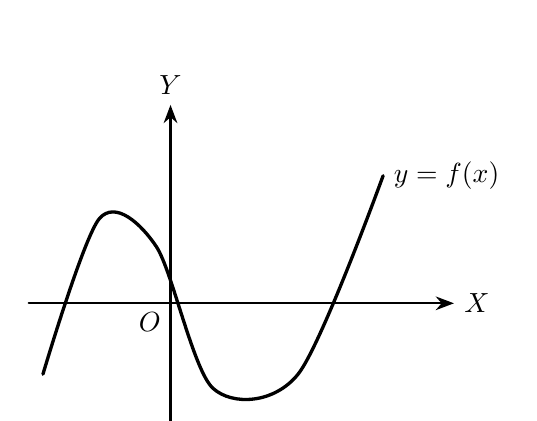
\begin{tikzpicture}[>=Stealth, scale=0.9, line cap=round, line join=round]
  \draw[->, thick] (-2.0, 0) -- (4.0, 0) node[right] {$X$};
  \draw[->, thick] (0, -1.8) -- (0, 2.8) node[above] {$Y$};
  \node[below left] at (0,0) {$O$};

  % Cubic curve crossing x axis 3 times
  \draw[very thick, smooth] plot coordinates {(-1.8, -1.0) (-1.0, 1.2) (-0.2, 0.8) (0.6, -1.2) (1.8, -1.0) (3.0, 1.8)} node[right] {$y=f(x)$};
\end{tikzpicture}
\end{figure}

此圖形與 $x$ 軸的交點在那裡？有多少交點？這些問題以代數的講法就是解聯立方程式
\[ \begin{cases} y = f(x) \\ y = 0 \end{cases} \]
此聯立方程式可以更簡便地記作 $f(x)=0$，而稱為\textbf{方程式}。如
\begin{align*}
\text{指數方程式：}& 5^{x+1} - 3 = 0, \\
\text{三角方程式：}& \sin 2x - 1 = 0, \\
\text{整式方程式：}& 5x^2 + 7x + 1 = 0, \\
\text{分式方程式：}& \dfrac{5x^2+7}{x+1} + \dfrac{6x+1}{x^3+1} + 1 = 0 \text{。}
\end{align*}
求滿足方程式中未知數的值就是解方程式。在方程式論裡我們只討論\textbf{多項式方程式}的求解。

要注意：函數討論的重點在於變量 $x$ 與 $y$ 間的關係，而相應的方程式 $f(x)=0$ 另有不同的意義。當然函數 $y=f(x)$ 與方程式 $f(x)=0$ 之間有相當密切的關係，二者在本章節中經常相互出現。又我們常把多項式與多項式函數二名稱不給以區別。讀者必能容易看出前者 $y=a_0 x^n + a_1 x^{n-1} + \dots + a_n$ 只表示 $x$ 為不定元，而用加，乘做出來的式子，後者意味著有函數對應關係，即給定一 $x=a$ 之值，有一確定的 $y$ 值與之對應。在實係數或複係數上此二者可以不加以區別的。

\subsubsection*{甲、一元 n 次方程式}\label{subsec:b6s-2-1-a}

任給一多項式 $f(x) = a_n x^n + a_{n-1} x^{n-1} + \dots + a_1 x + a_0$，其中 $a_n \ne 0$，則 $f(x)=0$ 稱為\textbf{一元 $n$ 次方程式}。根據這樣的定義，我們可以寫出 $n=1, 2, 3, 4, \dots$ 時的一元方程式：
\begin{align*}
\text{一次的：}& a_1 x + a_0 = 0 \\
\text{二次的：}& a_2 x^2 + a_1 x + a_0 = 0 \\
\text{三次的：}& a_3 x^3 + a_2 x^2 + a_1 x + a_0 = 0 \\
&\dots\dots\dots\dots
\end{align*}
一元 $n$ 次方程式論的中心課題在於討論根的求法，根與係數的關係等。因此對於其係數所在的範圍必須要有較明確的說明。為區別起見，當係數 $a_i$ ($i=0, \dots, n$) 皆為複數，稱為\textbf{複係數方程式}，當係數 $a_i$ 皆為實數，則稱為\textbf{實係數方程式}，仿此，如果 $a_i$ 皆為有理數，則稱為\textbf{有理係數方程式}。顯然

\begin{center}
\begin{tikzpicture}[>=Stealth, scale=0.9, line cap=round, line join=round]
  % Ellipse: 複係數方程式
  \draw[thick] (1.6, 0.9) ellipse (1.6cm and 0.78cm);
  \node at (1.6, 0.9) {複係數方程式};

  \node at (3.75, 0.9) {$\supset$};

  % Rectangle: 實係數方程式
  \draw[thick] (4.3, 0.12) rectangle (7.4, 1.68);
  \node at (5.85, 0.9) {實係數方程式};

  \node at (7.95, 0.9) {$\supset$};

  % Triangle: 有理係數方程式 (matching original p.82)
  \draw[thick] (8.45, 0.02) -- (12.25, 0.02) -- (10.35, 2.02) -- cycle;
  \node[align=center, font=\small] at (10.35, 0.68) {有理\\係數方程式};
\end{tikzpicture}
\end{center}

本章中如無特別指明係數所在的範圍，則所討論者皆為複係數方程式。

\begin{definition}\label{def:b6s-2-1}
對於 $n$ 次方程式 $f(x) = a_n x^n + a_{n-1} x^{n-1} + \dots + a_0 = 0$ 若有一數 $\alpha$，使得
\[ f(\alpha) = a_n \alpha^n + a_{n-1} \alpha^{n-1} + \dots + a_0 = 0 \]
則稱 $\alpha$ 為此方程式之\textbf{一根}。
\end{definition}

第一冊第五章所講的餘式定理，可推廣至複係數多項式。其中一個重要的推論可重述如下：

\begin{corollary}[因式定理]\label{cor:b6s-2-1}
設 $f(x)=0$ 為 $n$ 次方程式，若 $\alpha$ 為 $f(x)=0$ 之一根，則 $f(x)$ 能被 $x-\alpha$ 整除，反之若 $f(x) = (x-\alpha)g(x)$，（$g(x)$ 為一多項式）則 $\alpha$ 為 $f(x)=0$ 之一根。
\end{corollary}

\begin{example}\label{ex:b6s-2-1}
已知 1 與 7 均為方程式 $x^4 - 17x^3 + 99x^2 - 223x + 140 = 0$ 之一根，試解此方程式。
\end{example}

\paragraph{【解】}
利用綜合除法，以 $x-1$ 除方程式之左端，再以 $x-7$ 除，其商如下：
\begin{center}
\renewcommand{\arraystretch}{1.2}
\begin{tabular}{rrrrr|r}
$1$ & $-17$ & $99$ & $-223$ & $140$ & $1$ \\
    & $+1$  & $-16$ & $+83$ & $-140$ & \\
\hline
$1$ & $-16$ & $83$ & $-140$ & $0$ & $7$ \\
    & $+7$  & $-63$ & $+140$ & & \\
\hline
$1$ & $-9$  & $20$ & $0$ & &
\end{tabular}
\end{center}
由此得
\begin{align*}
x^4 - 17x^3 + 99x^2 - 223x + 140 &= (x-1)(x-7)(x^2 - 9x + 20) \\
&= (x-1)(x-7)(x-4)(x-5)
\end{align*}
故其根有 $1, 7, 4, 5$。\hfill$\#$

\begin{example}\label{ex:b6s-2-2}
求一三次多項式函數 $y=f(x)$，使得 $f(1)=0, f(4)=0, f(-1)=0, f(3)=8$。
\end{example}

\paragraph{【解】}
設此函數為
\begin{equation}
f(x) = a_3 x^3 + a_2 x^2 + a_1 x + a_0 \label{eq:b6s-2-1-1}
\end{equation}
根據推論 1 知
\begin{equation}
f(x) = c(x-1)(x-4)(x+1) \label{eq:b6s-2-1-2}
\end{equation}
\[ 8 = f(3) = c(3-1)(3-4)(3+1) \]
得 $c = -1$。故所求的函數為
\begin{align*}
f(x) &= (-1)(x-1)(x-4)(x+1) \\
&= -x^3 + 4x^2 + x - 4
\end{align*}
\hfill$\#$

\subsubsection*{作業 1}\label{hw:b6s-2-1}
試解 $x - 9\sqrt{x} - 20 = 0$。

\subsubsection*{作業 2}\label{hw:b6s-2-2}
試求三次多項式 $y=f(x)$ 滿足 $f(1)=0, f(3)=0, f(-1)=0, f(4)=2$。

\subsubsection*{乙、插入法}\label{subsec:b6s-2-1-b}

三、四冊已說明兩點決定唯一一直線，即決定一個一次函數 $y=mx+b$，上段例 2 又述及給定四點 $(1, 0), (4, 0), (-1, 0), (3, 8)$，則可得一三次多項式其圖形通過此四點。我們不免聯想到：如果在平面上給定不同的 $n$ 個點 $(a_1, b_1), \dots, (a_n, b_n)$ 可否尋得一個 $n-1$ 次多項式 $f(x)$，使得 $f(a_i)=b_i$ 呢？現在先以三點為例：

假設 $(a_1, b_1), (a_2, b_2), (a_3, b_3)$ 為給定三點，$a_1, a_2, a_3$ 互異。首先假設
\[ g_1(x) = c_1(x-a_2)(x-a_3) \]
其中 $c_1$ 為未定常數，我們希望適當地取 $c_1$ 使得 $g_1(a_1)=b_1$，如此必然要有
\[ c_1 = \dfrac{b_1}{(a_1-a_2)(a_1-a_3)} \]
同理另外可取定二函數 $g_2(x), g_3(x)$ 為
\begin{align*}
g_2(x) &= \dfrac{b_2(x-a_1)(x-a_3)}{(a_2-a_1)(a_2-a_3)}, \quad g_2(a_2)=b_2, \quad g_2(a_1)=g_2(a_3)=0 \\
g_3(x) &= \dfrac{b_3(x-a_2)(x-a_1)}{(a_3-a_2)(a_3-a_1)}, \quad g_3(a_3)=b_3, \quad g_3(a_1)=g_3(a_2)=0
\end{align*}
令 $f(x) = g_1(x) + g_2(x) + g_3(x)$，則 $f(x)$ 為所求的二次式，因為
\begin{align*}
f(a_1) &= g_1(a_1) + g_2(a_1) + g_3(a_1) = g_1(a_1) + 0 + 0 = b_1 \\
f(a_2) &= g_1(a_2) + g_2(a_2) + g_3(a_2) = 0 + g_2(a_2) + 0 = b_2 \\
f(a_3) &= g_1(a_3) + g_2(a_3) + g_3(a_3) = 0 + 0 + g_3(a_3) = b_3
\end{align*}
上述的方法稱為 \textbf{Lagrange（拉格蘭日）插入法}，推廣到 $n$ 點的情形則為：

\begin{theorem}[Lagrange's 插入法]\label{thm:b6s-2-lagrange}
設 $a_1, \dots, a_n$ 為 $n$ 個不同數，$b_1, \dots, b_n$ 為另一組 $n$ 個數。令
\[ P_i(x) = b_i \dfrac{(x-a_1)\dots(x-a_{i-1})(x-a_{i+1})\dots(x-a_n)}{(a_i-a_1)\dots(a_i-a_{i-1})(a_i-a_{i+1})\dots(a_i-a_n)} \]
則
\[ f(x) = P_1(x) + \dots + P_i(x) + \dots + P_n(x) \]
為 $n-1$ 次多項式且滿足 $f(a_i)=b_i, \quad i=1, \dots, n$。
\end{theorem}

\begin{example}\label{ex:b6s-2-3}
求一次數最低的多項式 $f(x)$ 使能滿足 $f(-1)=-6, f(0)=2, f(1)=-2, f(2)=6$。
\end{example}

\paragraph{【解】}
令
\begin{align*}
P_1(x) &= \dfrac{-6(x-0)(x-1)(x-2)}{(-1-0)(-1-1)(-1-2)} = x(x-1)(x-2) \\
P_2(x) &= \dfrac{2(x+1)(x-1)(x-2)}{(0+1)(0-1)(0-2)} = (x+1)(x-1)(x-2) \\
P_3(x) &= \dfrac{-2(x+1)(x-0)(x-2)}{(1+1)(1-0)(1-2)} = (x+1)x(x-2) \\
P_4(x) &= \dfrac{6(x+1)(x-0)(x-1)}{(2+1)(2-0)(2-1)} = (x+1)x(x-1)
\end{align*}
則
\begin{align*}
f(x) &= x(x-1)(x-2) + (x+1)(x-1)(x-2) \\
&\quad + (x+1)x(x-2) + (x+1)x(x-1) \text{ 為所求。}
\end{align*}
\hfill$\#$

\subsubsection*{作業 3}\label{hw:b6s-2-3}
試求一多項式 $f(x)$ 使能滿足 $f(1)=6, f(2)=3, f(-1)=-2, f(0)=1$。

\subsubsection*{習題 II-1}\label{sec:b6s-ex2-1}

\begin{enumerate}[label=\arabic*., leftmargin=2em]
  \item 令 $f(x)=a_0 x^n + \dots + a_n$，試證下列各題：
  \begin{enumerate}[label=(\roman*)]
    \item 若 $a_n=0$，則 $f(x)=0$ 有一根為 0，若 $a_n=a_{n-1}=0$ 則 $f(x)=0$ 有二根為 0，餘類推。
    \item 若 $a_0+a_1+\dots+a_n=0$，則 $f(x)=0$ 有 1 的根。
    \item 若 $a_0-a_1+\dots+(-1)^n a_n=0$，則 $f(x)=0$ 有 $-1$ 的根。
    \item 若 $a_i \ge 0$ ($i=0, 1, \dots, n$)，則 $f(x)=0$ 無正根。
    \item 若 $f(x)$ 的各項係數為正負相間，則 $f(x)=0$ 無負根。
  \end{enumerate}

  \item 試證 5 為 $f(x)=x^3-28x+15=0$ 的一根，試解 $f(x)=0$。

  \item 已知 $f(x)=0$ 有 $2, 1+i, 1-i$ 三根，$f(1)=2$ 試求 $f(x)$。

  \item 試證 $2x^3+3x^2-4x+5=0$ 的各根不大於 1。

  \item 試證 $x^3-2x^2-2x+1=0$ 及 $x^4-7x^2+1=0$ 有二根相同，並求各根。

  \item 解 $x^4+8x^3+18x^2-27=0$。

  \item 解 $(x-a)(x+2a)(x-3a)(x+4a)-24a^4=0$。

  \item 解 $x(x-1)(x-2)(x-3)-4 \cdot 3 \cdot 2 \cdot 1=0$。

  \item 解 $(a-x)^4+(x-b)^4-(a-b)^4=0$。

  \item 解
  \[ x^3 - a^3 \dfrac{(x-b)(x-c)}{(a-b)(a-c)} - b^3 \dfrac{(x-c)(x-a)}{(b-c)(b-a)} - c^3 \dfrac{(x-a)(x-b)}{(c-a)(c-b)} = 0 \]

  \item 試求滿足下列各條件次數最低的多項式：
  \begin{enumerate}[label=(\roman*)]
    \item $f(-1)=3, f(2)=f(1)=f(-5)=0$。
    \item $f(1)=2, f(2)=3, f(3)=4, f(4)=5$。
  \end{enumerate}

  \item 設 $c_1, \dots, c_k$ 為不同之數，取一 $j \in \{1, 2, \dots, k\}$ 令
  \[ p_j(x) = \dfrac{(x-c_1)\dots(x-c_{j-1})(x-c_{j+1})\dots(x-c_k)}{(c_j-c_1)\dots(c_j-c_{j-1})(c_j-c_{j+1})\dots(c_j-c_k)} \]
  \begin{enumerate}[label=(\roman*)]
    \item 試證 $x = c_1 p_1(x) + c_2 p_2(x) + \dots + c_k p_k(x)$。
    \item 設 $g(x)$ 為次數小於 $k-1$ 之多項式，則
    \[ g(x) = g(c_1)p_1(x) + \dots + g(c_k)p_k(x) \]
  \end{enumerate}
\end{enumerate}

\subsection{代數的基本定理}\label{sec:b6s-2-2}
\resetsectcounters

\subsubsection*{甲、複係數方程式}\label{subsec:b6s-2-2-a}

令 $f(x) = a_n x^n + a_{n-1} x^{n-1} + \dots + a_0 = 0$ 為 $n$ 次方程式，由因式定理知如果 $c_1, c_2, \dots, c_r$ 為 $f(x)$ 之根，則
\[ f(x) = (x-c_1)(x-c_2)\dots(x-c_r)f_r(x) \]
比較兩邊的次數，得 $f_r(x)$ 為 $n-r$ 次多項式。這樣的 $f_r(x)=0$ 稱為 $f(x)=0$ 的\textbf{降冪方程式}。如果 $c_{r+1}$ 是 $f_r(x)=0$ 之一根，再用一次因式定理於 $f_r(x)=0$，得
\[ f(x) = (x-c_1)\dots(x-c_r)(x-c_{r+1})f_{r+1}(x) \]
所以降冪方程式的根，仍是原方程式的根。

\begin{theorem}\label{thm:b6s-2-roots-bound}
設 $f(x)$ 為一個 $n$ 次多項式，則 $f(x)=0$ 至多有 $n$ 個根。
\end{theorem}

\begin{proof}[【證明】]
因為一個 $n$ 次多項式，不能被一個 $n+1$ 次的多項式整除。
\end{proof}\hfill$\#$

上面的結論仍然有缺點，因不能得知方程式的根是否存在。大家都知道 $x^2+1=0$ 沒有實數根（因為實數的平方永遠為非負，加 1 後絕不等於 0），如果擴大數的範圍，則可設一「數」$i$ 滿足此方程式。但是這僅是一個特例，方程式有無很多，是否每次都得把數的範圍無窮次地擴展，引進新的數做為它們的根呢？這問題在十八世紀已由大數學家\textbf{高斯（Gauss）}得到解決，今述之如下。定理的證明（現已有很多種），需要更多的數學工具，而超出本書之範圍，故予從略。

\begin{theorem}[代數的基本定理]\label{thm:b6s-2-fta}
令 $f(x)$ 為 $n$ 次多項式，則 $f(x)=0$ 至少有一複數為其根。
\end{theorem}

\begin{corollary}\label{cor:b6s-2-n-roots}
$n$ 次方程式 $f(x)=0$ 恰有 $n$ 個複數根。
\end{corollary}

\begin{discussion}\label{disc:b6s-2-1}
任一複數開平方仍然是複數。
\end{discussion}

\begin{proof}[【證明】]
複數 $a+bi$ ($ab \ne 0$) 開平方，就是要求 $x^2-(a+bi)=0$ 的根。根據推論 1 知此方程式有兩個複數根。實際上 $\sqrt{a+bi}$ 的求法是這樣的，設
\[ \sqrt{a+bi} = x+yi \]
兩邊平方，得
\[ a+bi = (x+yi)^2 = x^2-y^2 + 2xyi \]
故有
\[ \begin{cases} a = x^2-y^2 \\ b = 2xy \end{cases} \]
求解此聯立方程式，得二組 $x, y$（第四冊第五章複數系已述及）。
\end{proof}\hfill$\#$

\begin{example}\label{ex:b6s-2-4}
試求 $z^2+5z+a+bi=0$ 有二實根之充要條件，其中 $a, b$ 為實數。
\end{example}

\paragraph{【解】}
其根為
\[ z = \dfrac{-5 \pm \sqrt{25 - 4(a+bi)}}{2} \]
此為實數當且僅當 $\sqrt{25 - 4(a+bi)}$ 為實數。設 $\sqrt{25 - 4(a+bi)} = x$，若 $x$ 為實數，則因
\[ 25 - 4a - 4bi = x^2 \]
必有 $b=0$ 及 $25-4a = x^2 \ge 0 \implies \dfrac{25}{4} \ge a$。故其充要條件為 $b=0, \dfrac{25}{4} \ge a$。\hfill$\#$

\subsubsection*{作業 4}\label{hw:b6s-2-4}
\begin{enumerate}[label=(\roman*), leftmargin=2em]
  \item 求 $\sqrt{1+i}$。
  \item 已知方程式 $x^3 - (i+1)x^2 + (i-20)x + 20i = 0$ 有一根為 5，求解此方程式。
  \item 已知方程式 $x^2 + 2(1+i)x + a + bi = 0$ 有一實根為 2，試求 $a, b$ 且解此方程式。
\end{enumerate}

\subsubsection*{乙、實係數方程式}\label{subsec:b6s-2-2-b}

$a+bi$ ($a, b$ 為實數) 的共軛數為 $a-bi$，二數的乘積為 $a^2+b^2$，和為 $2a$，以此二數為根做一方程式得 $x^2 - 2ax + a^2 + b^2 = 0$，反之，設 $x^2 + Cx + D = 0$ 為一個二次實係數方程式，如果它有一複數根 $a+bi$，則其共軛數 $a-bi$ 亦必為它的一根，這一現象是下述定理的特例：

\begin{theorem}[虛根共軛定理]\label{thm:b6s-2-conjugate}
實係數方程式 $a_n x^n + a_{n-1} x^{n-1} + \dots + a_1 x + a_0 = 0$ 若有一複數根 $a+bi$，則其共軛數 $a-bi$ 亦為其根，其中 $a, b$ 為實數。
\end{theorem}

\begin{proof}[【證明】]
我們知道：
\begin{enumerate}[label=(\roman*), leftmargin=2em]
  \item 二複數乘積的共軛數，等於各個共軛數的乘積：$\bar{z_1 z_2} = \bar{z}_1 \bar{z}_2$。推論可得 $\bar{z_1 z_2 \dots z_n} = \bar{z}_1 \bar{z}_2 \dots \bar{z}_n$。又 $\bar{az} = a\bar{z}, \quad a \in \mathbb{R}$。
  \item 二複數和之共軛數等於各個共軛數之和：$\bar{z_1 + z_2} = \bar{z}_1 + \bar{z}_2$。
\end{enumerate}
由 (i) (ii) 知
\begin{align*}
\bar{f(z)} &= \bar{a_n z^n + a_{n-1} z^{n-1} + \dots + a_0} \\
&= a_n (\bar{z})^n + a_{n-1} (\bar{z})^{n-1} + \dots + a_0 = f(\bar{z})
\end{align*}
如果 $\alpha = a+bi$ 為 $f(x)=0$ 之一根，則
\[ f(\alpha) = a_n \alpha^n + a_{n-1} \alpha^{n-1} + \dots + a_0 = 0 \]
因此
\begin{align*}
0 = \bar{0} = \bar{f(\alpha)} &= a_n (\bar{\alpha})^n + a_{n-1} (\bar{\alpha})^{n-1} + \dots + a_1 (\bar{\alpha}) + a_0 = f(\bar{\alpha})
\end{align*}
故 $\bar{\alpha}$ 亦為 $f(x)=0$ 之一根。
\end{proof}\hfill$\#$

\begin{corollary}\label{cor:b6s-2-real-factor}
實係數多項式 $f(x)$ 在實數範圍內可分解為實係數一次式及二次式的乘積。
\end{corollary}

\begin{proof}[【證明】]
令 $f(x)=0$ 的複數根為 $\alpha_1, \bar{\alpha}_1, \alpha_2, \bar{\alpha}_2, \dots, \alpha_r, \bar{\alpha}_r$，實數根為 $\beta_1, \beta_2, \dots, \beta_s$ ($2r+s=n$) 則
\begin{align*}
f(x) &= a_n (x-\alpha_1)(x-\bar{\alpha}_1)\dots(x-\alpha_r)(x-\bar{\alpha}_r)(x-\beta_1)\dots(x-\beta_s) \\
&= a_n [x^2 - (\alpha_1+\bar{\alpha}_1)x + \alpha_1\bar{\alpha}_1]\dots[x^2 - (\alpha_r+\bar{\alpha}_r)x + \alpha_r\bar{\alpha}_r](x-\beta_1)\dots(x-\beta_s)
\end{align*}
因為 $\alpha_i+\bar{\alpha}_i, \alpha_i\bar{\alpha}_i, \beta_j$ 皆為實數，故以上二次因式均為實係數，即 $f(x)$ 可分解成實係數一次式及二次式的乘積。
\end{proof}\hfill$\#$

\begin{discussion}\label{disc:b6s-2-2}
一個 $n$ 次實係數多項式 $y=f(x)$ 與一直線最多交於 $n$ 點。
\end{discussion}

\begin{proof}[【證明】]
設一直線方程式為 $y=mx+b$。

\begin{figure}[H]
\centering
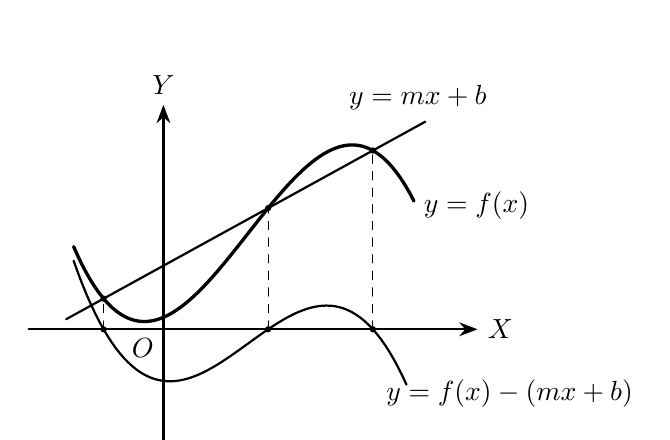
\begin{tikzpicture}[>=Stealth, scale=0.95, line cap=round, line join=round]
  \draw[->, thick] (-1.8, 0) -- (4.2, 0) node[right] {$X$};
  \draw[->, thick] (0, -1.6) -- (0, 3.0) node[above] {$Y$};
  \node[below left] at (0,0) {$O$};

  % Line y = mx + b: y = 0.55x + 0.85
  \draw[thick, domain=-1.3:3.5] plot (\x, {0.55*\x + 0.85});
  \node[above] at (3.4, 2.8) {$y=mx+b$};

  % Difference curve d(x) = -0.22*(x+0.8)*(x-1.4)*(x-2.8)
  % Intersects x-axis at x = -0.8, 1.4, 2.8
  \draw[thick, domain=-1.2:3.25, samples=80]
    plot (\x, {-0.22*(\x+0.8)*(\x-1.4)*(\x-2.8)});
  \node[below right] at (2.85, -0.55) {$y=f(x)-(mx+b)$};

  % Curve y = f(x) = mx + b + d(x)
  \draw[very thick, domain=-1.2:3.35, samples=80]
    plot (\x, {0.55*\x + 0.85 - 0.22*(\x+0.8)*(\x-1.4)*(\x-2.8)});
  \node[right] at (3.35, 1.65) {$y=f(x)$};

  % Vertical dashed lines at intersection x-coordinates
  \foreach \xi in {-0.8, 1.4, 2.8} {
    \draw[dashed] (\xi, 0) -- (\xi, {0.55*\xi + 0.85});
    \fill (\xi, 0) circle (1.2pt);
    \fill (\xi, {0.55*\xi + 0.85}) circle (1.2pt);
  }
\end{tikzpicture}
\end{figure}

解
\[ \begin{cases} y = f(x) \\ y = mx+b \end{cases} \]
即 $f(x) - mx - b = 0$ 此為 $n$ 次方程式，最多只有 $n$ 個根，故 $y=f(x)$ 與 $y=mx+b$ 最多交 $n$ 點。
\end{proof}\hfill$\#$

\begin{discussion}\label{disc:b6s-2-3}
設實係數方程式 $f(x) = a_n x^n + a_{n-1} x^{n-1} + \dots + a_0, f(x)=0$ 無實根，而且 $a_n > 0$ 則對於任意 $x \in \mathbb{R}$，有 $f(x) \ge 0$。
\end{discussion}

\begin{proof}[【證明】]
$f(x) = a_n \{ x^2 - (\alpha_1+\bar{\alpha}_1)x + \alpha_1\bar{\alpha}_1 \} \dots \{ x^2 - (\alpha_r+\bar{\alpha}_r)x + \alpha_r\bar{\alpha}_r \}$。今觀察其中一個因式
\[ h_j(x) = x^2 - (\alpha_j+\bar{\alpha}_j)x + \alpha_j\bar{\alpha}_j \]
令 $\alpha_j = a_j + b_j i$ 則
\[ h_j(x) = x^2 - 2a_j x + a_j^2 + b_j^2 = (x-a_j)^2 + b_j^2 \]
如 $x$ 為實數，$(x-a_j)^2 + b_j^2 \ge 0$。因此對於 $x \in \mathbb{R}$，$f(x)$ 之各因式皆為 $\ge 0$。
\end{proof}\hfill$\#$

\begin{example}\label{ex:b6s-2-5}
設 $f(x)=ax^2+bx+c=0$ 當 $b^2-4ac < 0$ 時，$ax^2+bx+c=0$ 無實根，故 $a f(x) \ge 0$。
\end{example}

\begin{proof}[【證】]
由配方法得
\[ f(x) = ax^2+bx+c = a \left[ \left(x+\dfrac{b}{2a}\right)^2 - \dfrac{b^2-4ac}{4a^2} \right] \]
$f(x)=0$ 無實根，則表示 $b^2-4ac < 0$，故 $f(x)$ 的值與 $a$ 的值同號。

\begin{figure}[H]
\centering
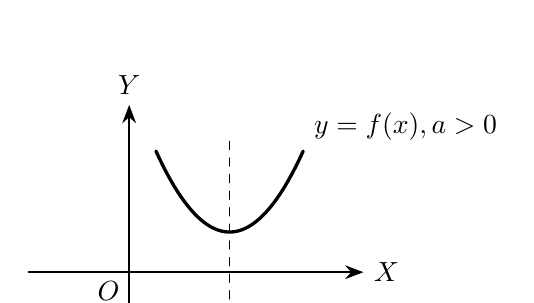
\begin{tikzpicture}[>=Stealth, scale=0.85, line cap=round, line join=round]
  \draw[->, thick] (-1.5, 0) -- (3.5, 0) node[right] {$X$};
  \draw[->, thick] (0, -0.6) -- (0, 2.5) node[above] {$Y$};
  \node[below left] at (0,0) {$O$};

  % Parabola completely above x-axis
  \draw[very thick, domain=0.4:2.6, samples=50] plot (\x, {(\x-1.5)^2 + 0.6}) node[above right] {$y=f(x), a>0$};
  \draw[dashed] (1.5, -0.4) -- (1.5, 2.0);
\end{tikzpicture}
\end{figure}
從幾何觀點說，$f(x)=0$ 無實根，即表示 $y=f(x)$ 的圖形與 $x$ 軸不相交，即拋物線不是在 $x$ 軸上方，便是在 $x$ 軸下方。
\end{proof}\hfill$\#$

\subsubsection*{作業 5}\label{hw:b6s-2-5}
設一個 $2n$ 次方程式為
\[ f(x) = a_{2n} x^{2n} + a_{2(n-1)} x^{2(n-1)} + \dots + a_{2i} x^{2i} + \dots + a_2 x^2 + a_0 = 0 \]
如果 $f(x)=0$ 有一根為 $\alpha$，試證 $-\alpha$ 亦為其根。

\subsubsection*{丙、函數之圖示}\label{subsec:b6s-2-2-c}

在三、四冊裡讀者已熟悉幾何與代數的轉換關係，如一次多項式函數可繪出直線，二次多項式函數可繪出拋物線等等。對於一個實係數多項式 $y=f(x)$，給定一實數 $x=a$，有一確定的對應值 $y=b=f(a)$，如此在 $xy$ 平面上就有一對應點 $(a, b)$。

\begin{figure}[H]
\centering
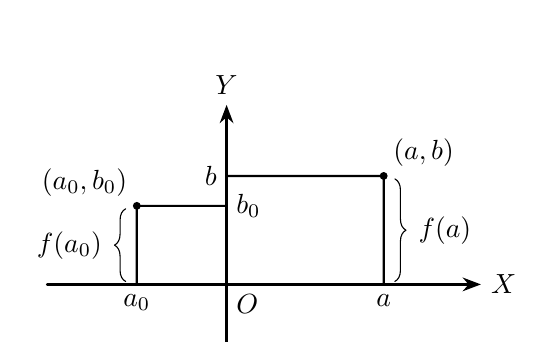
\begin{tikzpicture}[>=Stealth, scale=0.95, line cap=round, line join=round]
  \draw[->, thick] (-2.4, 0) -- (3.4, 0) node[right] {$X$};
  \draw[->, thick] (0, -0.9) -- (0, 2.4) node[above] {$Y$};
  \node[below right] at (0,0) {$O$};

  \coordinate (A0) at (-1.2, 1.05);
  \coordinate (A) at (2.1, 1.45);

  \draw[thick] (-1.2, 0) node[below] {$a_0$} -- (A0) -- (0, 1.05);
  \draw[thick] (2.1, 0) node[below] {$a$} -- (A) -- (0, 1.45);

  \fill (A0) circle (1.5pt) node[above left] {$(a_0, b_0)$};
  \fill (A) circle (1.5pt) node[above right] {$(a, b)$};
  \node[right] at (0, 1.05) {$b_0$};
  \node[left] at (0, 1.45) {$b$};

  % Braces matching original p.91
  \draw[decorate, decoration={brace, amplitude=4pt}] (-1.35, 0.04) -- (-1.35, 1.01) node[midway, left=5pt] {$f(a_0)$};
  \draw[decorate, decoration={brace, amplitude=4pt}] (2.25, 1.41) -- (2.25, 0.04) node[midway, right=5pt] {$f(a)$};
\end{tikzpicture}
\end{figure}

如果 $x$ 在 $X$ 軸上移動，就得到許多與之相對應的點，把這些點（圓滑地）描繪起來，稱為此函數之圖示。嚴格地說，我們必須描出當 $x$ 變動時所有的平面上的對應點的軌跡，才能確切地表出此函數之曲線。有時函數簡單，則不必那麼費事，如二點就可決定一直線。我們描述多項式亦可照著大略情形而繪的。

\begin{example}\label{ex:b6s-2-6}
$y = x^3$
\end{example}

\begin{center}
\small
\renewcommand{\arraystretch}{1.2}
\begin{tabular}{|c|c|c|c|c|c|c|c|c|c|c|c|}
\hline
$x$ & $-5$ & $-4$ & $-3$ & $-2$ & $-1$ & $0$ & $1$ & $2$ & $3$ & $4$ & $5$ \\ \hline
$f(x)$ & $-125$ & $-64$ & $-27$ & $-8$ & $-1$ & $0$ & $1$ & $8$ & $27$ & $64$ & $125$ \\ \hline
\end{tabular}
\end{center}

\begin{figure}[H]
\centering
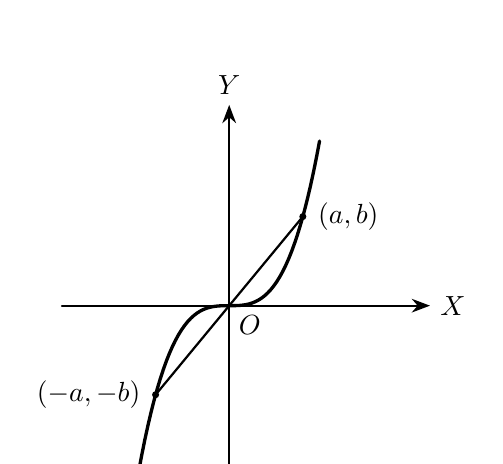
\begin{tikzpicture}[>=Stealth, scale=0.85, line cap=round, line join=round]
  \draw[->, thick] (-2.5, 0) -- (3.0, 0) node[right] {$X$};
  \draw[->, thick] (0, -2.5) -- (0, 3.0) node[above] {$Y$};
  \node[below right] at (0,0) {$O$};

  \draw[very thick, domain=-1.35:1.35, samples=60] plot (\x, {\x*\x*\x});
  % Symmetry secant line through origin (matching original p.91)
  \draw[thick] (-1.1, -1.331) -- (1.1, 1.331);
  \fill (1.1, 1.331) circle (1.5pt) node[right=2pt] {$(a, b)$};
  \fill (-1.1, -1.331) circle (1.5pt) node[left=2pt] {$(-a, -b)$};
\end{tikzpicture}
\end{figure}

繪圖時需要特別注意：
\begin{enumerate}[label=(\arabic*), leftmargin=2em]
  \item 對稱性
  \item 與 $X, Y$ 軸的交點（$X$ 截距，$Y$ 截距）
  \item 極大極小
  \item 曲線的升降
\end{enumerate}

\begin{example}\label{ex:b6s-2-7}
$y = 2x^2 - x^4$
\end{example}

因為 $f(x)=f(-x)$，所以函數對於 $Y$ 軸對稱，我們只需討論 $x \ge 0$ 的情形：

\begin{center}
\small
\renewcommand{\arraystretch}{1.2}
\begin{tabular}{|c|c|c|c|c|c|c|}
\hline
$x$ & $0$ & $\dfrac{1}{2}$ & $1$ & $\sqrt{2}$ & $2$ & $3$ \\ \hline
$f(x)$ & $0$ & $\dfrac{7}{16}$ & $1$ & $0$ & $-8$ & $-63$ \\ \hline
\end{tabular}
\end{center}

$y = 1 - (1-2x^2+x^4) = 1 - (1-x^2)^2$，故此函數在 $x=1$ 取得最大值，$x \longrightarrow \infty$ 時 $f(x)$ 趨於負無窮大。

\begin{figure}[H]
\centering
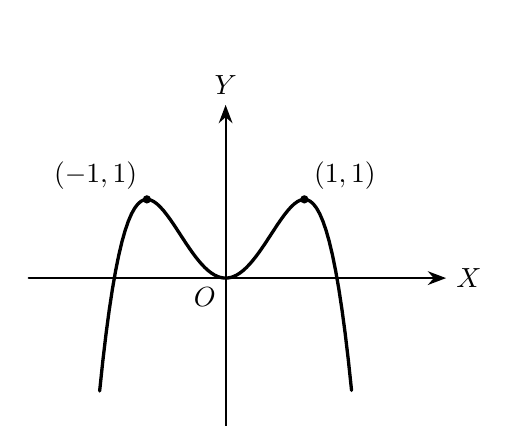
\begin{tikzpicture}[>=Stealth, scale=1.0, line cap=round, line join=round]
  \draw[->, thick] (-2.5, 0) -- (2.8, 0) node[right] {$X$};
  \draw[->, thick] (0, -2.0) -- (0, 2.2) node[above] {$Y$};
  \node[below left] at (0,0) {$O$};

  % M-curve: y = 2x^2 - x^4
  \draw[very thick, domain=-1.6:1.6, samples=80] plot (\x, {2*\x*\x - \x*\x*\x*\x});
  \fill (1, 1) circle (1.5pt) node[above right] {$(1, 1)$};
  \fill (-1, 1) circle (1.5pt) node[above left] {$(-1, 1)$};
\end{tikzpicture}
\end{figure}
\hfill$\#$

\subsubsection*{作業 6}\label{hw:b6s-2-6}
試描繪下列各函數的曲線：
\begin{multicols}{2}
\begin{enumerate}[label=(\roman*)]
  \item $y = x^4$
  \item $y = x - x^3$
\end{enumerate}
\end{multicols}

\subsubsection*{習題 II-2}\label{sec:b6s-ex2-2}

\begin{enumerate}[label=\arabic*., leftmargin=2em]
  \item 試求 $\sqrt{3-4i}$。
  \item 試解下列複數方程式：
  \begin{enumerate}[label=(\roman*)]
    \item $2z^4 - 2iz^3 + z^2 + 1 = 0$
    \item $z^3 + (1+i)z - (10+2i) = 0$
    \item $z^3 + (1+2i)z^2 - 3(1+2i)z + 1 + 4i = 0$
  \end{enumerate}
  \item 試作出一方程式以 $3, 2-i, 1+i$ 為根。
  \item 已知 $\omega = \dfrac{-1+\sqrt{3}i}{2}$ 為 $x^4+4x^3+8x^2+7x+4=0$ 的一根，試解方程式。
  \item 已知 $\sqrt{3}+\sqrt{2}i$ 為 $f(x)=0$ 的一根，試求最低次整係數方程式。
  \item 試解 $x^5+2x^4-3x^3-3x^2+2x+1=0$。
  \item 試分解 $f(x)=x^3+x^2+x+1$ 為一次或二次因式的乘積。
  \item 試分解 $f(x)=x^4-5x^3+4x^2-5x+1$ 為一次或二次因式的乘積。
  \item 試求出曲線 $y=x^3+4x+2$ 與直線 $y=x-2$ 的交點。
  \item 試解 $[x]^2+[x]-6=0$（$[x]$ 為高斯函數）。
  \item 若 $a, b, c$ 為正數，試證 $a^3+b^3+c^3 \ge 3abc$。
  \item 試證對於所有實數 $x$，$x^8+x^4+1 > 0$。
  \item 試繪出下列各函數的曲線：
  \begin{multicols}{2}
  \begin{enumerate}[label=(\roman*)]
    \item $y = 3 - 5x - x^2$
    \item $y = x^3 + 3x$
    \item $y = 2x^3 - 3x^2$
    \item $y = x^3 + x + 2$
    \item $y = x^4 - 4x$
    \item $y = x^4 - 2x^2$
    \item $y = x^4 - x^3$
    \item $y = x^4 - 2x + 1$
  \end{enumerate}
  \end{multicols}
\end{enumerate}

\subsection{根與係數的關係與對稱式}\label{sec:b6s-2-3}
\resetsectcounters

\subsubsection*{甲、根與係數的關係}\label{subsec:b6s-2-3-a}

在本書第一冊第七章裡有這樣一個定理：設 $\dfrac{b}{c}$ 是整係數方程式 $f(x) = a_n x^n + a_{n-1} x^{n-1} + \dots + a_0 = 0$ 的一個有理根，其中 $c > 0$，且 $(b, c)=1$ 則 $b$ 必定是 $a_0$ 的因數，$c$ 必定是 $a_n$ 的因數。上命題已指出一個有趣的事實：根與係數有密切的關係，特再舉一例來觀察：

設 $\beta_1, \beta_2, \beta_3$ 為方程式 $x^3 + a_1 x^2 + a_2 x + a_3 = 0$ 之三根，則有
\begin{align*}
x^3 + a_1 x^2 + a_2 x + a_3 &= (x-\beta_1)(x-\beta_2)(x-\beta_3) \\
&= x^3 - (\beta_1+\beta_2+\beta_3)x^2 + (\beta_1\beta_2+\beta_2\beta_3+\beta_3\beta_1)x - \beta_1\beta_2\beta_3
\end{align*}
比較兩邊係數得
\begin{align*}
a_1 &= -(\beta_1+\beta_2+\beta_3) \\
a_2 &= (\beta_1\beta_2+\beta_2\beta_3+\beta_3\beta_1) \\
a_3 &= -\beta_1\beta_2\beta_3
\end{align*}
更一般地觀察，令 $\beta_1, \beta_2, \dots, \beta_n$ 為方程式 $f(x) = x^n + a_1 x^{n-1} + a_2 x^{n-2} + \dots + a_{n-1} x + a_n = 0$ 之 $n$ 個根，則有
\[ f(x) = (x-\beta_1)(x-\beta_2)\dots(x-\beta_n) \]
展開右式後，比較兩端係數得
\begin{equation}
\begin{aligned}
a_1 &= -(\beta_1+\beta_2+\dots+\beta_n) = -(\text{所有根之和}) \\
a_2 &= \beta_1\beta_2+\beta_1\beta_3+\dots+\beta_1\beta_n+\beta_2\beta_3+\dots+\beta_{n-1}\beta_n = \text{所有根兩兩相乘所得之和} \\
a_3 &= -(\beta_1\beta_2\beta_3+\beta_1\beta_2\beta_4+\dots) = -(\text{所有根三三相乘所得之和}) \\
&\dots\dots\dots\dots \\
a_n &= (-1)^n \beta_1\beta_2\dots\beta_n = (-1)^n (\text{所有根之乘積})
\end{aligned} \tag{I} \label{eq:b6s-2-3-I}
\end{equation}
若 $n$ 次方程式 $a_0 x^n + a_1 x^{n-1} + \dots + a_n = 0$ 的首項係數 $a_0 \ne 1$ 我們以 $a_0$ 遍除各項，再把方程式的缺項，以 0 補足，可以得到下述定理：

\begin{theorem}[根與係數的關係 / 韋達定理]\label{thm:b6s-2-vieta}
設 $n$ 次方程式 $a_0 x^n + a_1 x^{n-1} + \dots + a_{n-1} x + a_n = 0$ 以 $\beta_1, \beta_2, \dots, \beta_n$ 為其根，則有
\begin{equation}
\begin{aligned}
\dfrac{a_1}{a_0} &= -(\beta_1+\dots+\beta_n) \\
\dfrac{a_2}{a_0} &= (\beta_1\beta_2+\dots+\beta_{n-1}\beta_n) \\
&\dots\dots\dots\dots \\
\dfrac{a_n}{a_0} &= (-1)^n \beta_1\beta_2\dots\beta_n
\end{aligned} \tag{II} \label{eq:b6s-2-3-II}
\end{equation}
\end{theorem}

\begin{example}\label{ex:b6s-2-8}
設 $x^3+7x^2-6x-72=0$ 有二根 3 與 $-4$，試求另一根。
\end{example}

\paragraph{【解】}
設 $3, -4, \beta$ 為此方程之三根，根據定理知
\[ 3(-4)\beta = (-1)^3(-72) = 72 \implies \beta = -6 \]\hfill$\#$

\begin{example}\label{ex:b6s-2-9}
設方程式 $x^3+ax^2+bx+c=0$ 之三根成等比，試證 $b^3-a^3c=0$。
\end{example}

\paragraph{【解】}
設此方程式的三根為 $\dfrac{\alpha}{\beta}, \alpha, \alpha\beta$，則根據根與係數的關係得
\begin{align*}
\dfrac{\alpha}{\beta} + \alpha + \alpha\beta &= -a \\
\dfrac{\alpha^2}{\beta} + \alpha^2 + \alpha^2\beta &= b \\
\dfrac{\alpha}{\beta} \cdot \alpha \cdot \alpha\beta &= -c
\end{align*}
即
\begin{align}
\alpha\left(\dfrac{1}{\beta}+1+\beta\right) &= -a \label{eq:b6s-2-3-ex2-1} \\
\alpha^2\left(\dfrac{1}{\beta}+1+\beta\right) &= b \label{eq:b6s-2-3-ex2-2} \\
\alpha^3 &= -c \label{eq:b6s-2-3-ex2-3}
\end{align}
$\dfrac{\eqref{eq:b6s-2-3-ex2-2}}{\eqref{eq:b6s-2-3-ex2-1}} \implies \alpha = -\dfrac{b}{a}$。代入 \eqref{eq:b6s-2-3-ex2-3} 得 $-\dfrac{b^3}{a^3} = -c$，故 $b^3 - a^3 c = 0$。\hfill$\#$

\subsubsection*{作業 7}\label{hw:b6s-2-7}
\begin{enumerate}[label=(\roman*), leftmargin=2em]
  \item 定義三階方陣 $\begin{pmatrix} a_{11} & a_{12} & a_{13} \\ a_{21} & a_{22} & a_{23} \\ a_{31} & a_{32} & a_{33} \end{pmatrix}$ 的特徵方程式為
  \[ \begin{vmatrix}
  a_{11}-x & a_{12} & a_{13} \\
  a_{21} & a_{22}-x & a_{23} \\
  a_{31} & a_{32} & a_{33}-x
  \end{vmatrix} = 0 \]
  試證此方程式諸根之和為 $(a_{11}+a_{22}+a_{33})$\phantomsection\label{note:b6s-ch2-p95-trace}\footnote{【原書校訂】：原書此處印作「$-(a_{11}+a_{22}+a_{33})$」，漏消負號（$(-x)^3 + (a_{11}+a_{22}+a_{33})x^2 + \dots = 0 \implies$ 根之和為 $a_{11}+a_{22}+a_{33}$），茲予校訂正號。}，諸根之積為 $\begin{vmatrix} a_{11} & a_{12} & a_{13} \\ a_{21} & a_{22} & a_{23} \\ a_{31} & a_{32} & a_{33} \end{vmatrix}$。
  \item 推廣 (i) 至 $n$ 階方陣。
\end{enumerate}

\subsubsection*{作業 8}\label{hw:b6s-2-8}
設方程式 $x^2+px+q=0$ 之二根為 $\alpha, \beta$，方程式 $x^2+Px+Q=0$ 之二根為 $\alpha(\alpha+1), \beta(\beta+1)$。試證
\[ P = p - p^2 + 2q, \qquad Q = q + q^2 - qp \]

\subsubsection*{*乙、對稱式基本定理}\label{subsec:b6s-2-3-b}

對於上小段的 (I) 式，我們可以引用一種簡單的符號：
\begin{align*}
\beta_1+\beta_2+\dots+\beta_n &= \sum_{i=1}^n \beta_i \\
\beta_1\beta_2+\dots+\beta_{n-1}\beta_n &= \sum_{i=1, j=2, i<j}^n \beta_i \beta_j \\
\beta_1\beta_2\beta_3+\beta_1\beta_2\beta_4+\dots &= \sum_{1 \le i_1 < i_2 < i_3 \le n} \beta_{i_1}\beta_{i_2}\beta_{i_3}
\end{align*}
注意到：在這些式子中，把任意二數 $\beta_i, \beta_j$ 對調，所得的結果不變。又 $\beta_1^2+\beta_2^2+\dots+\beta_n^2$ 亦有這樣的性質。

\begin{definition}\label{def:b6s-2-symmetric}
令 $P(x_1, \dots, x_n)$ 為一 $n$ 元多項式，如果在 $P(x_1, \dots, x_n)$ 中任意對調二不定元 $x_i, x_j$，所得的式子與原式相同，稱此多項式為\textbf{對稱多項式}或簡稱為\textbf{對稱式}。
\end{definition}

\begin{example}\label{ex:b6s-2-10}
\begin{enumerate}[label=(\arabic*), leftmargin=2em]
  \item $x^3+y^3+z^3-3xyz$ \dots 三元齊次對稱式
  \item $x_1^2 x_2 + x_1^2 x_3 + x_2^2 x_1 + x_2^2 x_3 + x_3^2 x_1 + x_3^2 x_2$ \dots 三元齊次對稱式
  \item $x_1^4+x_2^4+x_3^4+x_4^4+x_1+x_2+x_3+x_4$ \dots 四元對稱式
\end{enumerate}
\end{example}

\begin{example}\label{ex:b6s-2-11}
設方程式 $x^3+2x^2+7x+6=0$ 之三根為 $x_1, x_2, x_3$ 試求
\begin{multicols}{2}
\begin{enumerate}[label=(\roman*)]
  \item $x_1^2+x_2^2+x_3^2$
  \item $x_1^3+x_2^3+x_3^3$
\end{enumerate}
\end{multicols}
\end{example}

\paragraph{【解】}
\begin{enumerate}[label=(\roman*), leftmargin=2em]
  \item
  \begin{align*}
  x_1^2+x_2^2+x_3^2 &= (x_1+x_2+x_3)^2 - 2(x_1 x_2 + x_1 x_3 + x_2 x_3) \\
  &= (-2)^2 - 2 \cdot 7 = 4 - 14 = -10
  \end{align*}
  \item
  \begin{align*}
  x_1^3+x_2^3+x_3^3 &= x_1^3+x_2^3+x_3^3-3x_1 x_2 x_3 + 3x_1 x_2 x_3 \\
  &= (x_1+x_2+x_3)(x_1^2+x_2^2+x_3^2 - x_1 x_2 - x_1 x_3 - x_2 x_3) + 3x_1 x_2 x_3 \\
  &= (-2)(-10-7) + 3(-6) = 34 - 18 = 16
  \end{align*}
\end{enumerate}
\hfill$\#$

在上面例子中，我們將對稱多項式 (i), (ii) 表為某些簡單（或整齊些）的對稱多項式之有理式，而這些特別的對稱多項式，都是在 (I) 中出現的。是否任意對稱多項式都可以表成 (I) 中對稱多項式的有理式呢？這就是本節所要討論的。

設 $x_1, \dots, x_n$ 為不定元，令
\begin{equation}
\begin{aligned}
P_1 &= x_1 + \dots + x_n = \sum_{1 \le i \le n} x_i \\
P_2 &= x_1 x_2 + \dots + x_1 x_n + \dots + x_{n-1} x_n = \sum_{1 \le i < j \le n} x_i x_j \\
P_j &= \sum_{1 \le i_1 < i_2 < \dots < i_j \le n} x_{i_1}\dots x_{i_j} \\
&\dots\dots\dots\dots \\
P_n &= x_1 x_2 \dots x_n
\end{aligned} \tag{III} \label{eq:b6s-2-3-III}
\end{equation}
這些多項式稱為 \textbf{$n$ 元基本對稱多項式}。

讀者注意到：
\begin{enumerate}[label=(\arabic*), leftmargin=2em]
  \item 0 是一個對稱式。
  \item 任意二 $n$ 元對稱式的和、差、積仍是對稱式。更一般地說：設 $f_1, f_2, \dots, f_t$ 為 $t$ 個對稱式，以這 $t$ 個式子為不定元的任一多項式 $P(f_1, f_2, \dots, f_t)$ 仍然是對稱式。特別地以 \eqref{eq:b6s-2-3-III} 中的對稱式 $P_1, \dots, P_n$ 做出的任一多項式 $Q(P_1, \dots, P_n)$ 仍為對稱式。
  \item $P_1$ 是 $n$ 元一次式，$P_2$ 是二次式，\dots，$P_n$ 是 $n$ 次式。
  \item 令 $P_1', P_2', \dots, P_{n-1}'$ 是 $x_2, \dots, x_n$ 的 $n-1$ 元基本對稱式，則有
  \begin{equation}
  \begin{aligned}
  P_1 &= x_1 + x_2 + \dots + x_n = x_1 + P_1' \\
  P_2 &= x_1 x_2 + \dots + x_1 x_n + x_2 x_3 + \dots + x_{n-1} x_n = x_1 P_1' + P_2' \\
  P_i &= x_1 P_{i-1}' + P_i' \qquad i=2, \dots, n-1 \\
  &\dots\dots\dots\dots \\
  P_n &= x_1 P_{n-1}'
  \end{aligned} \tag{IV} \label{eq:b6s-2-3-IV}
  \end{equation}
  \item 下列等式成立：
  \begin{equation}
  x_1^n - P_1 x_1^{n-1} + P_2 x_1^{n-2} + \dots + (-1)^n P_n = 0 \tag{V} \label{eq:b6s-2-3-V}
  \end{equation}
\end{enumerate}

\begin{proof}[【證明】]
考慮一函數 $f(z) = (z-x_1)(z-x_2)\dots(z-x_n) = z^n - P_1 z^{n-1} + P_2 z^{n-2} + \dots + (-1)^n P_n$。因為 $f(x_1)=0$，故得上式。
\end{proof}

\begin{lemma}\label{lem:b6s-2-sym-vandermonde}
設 $b_0, b_1, \dots, b_{n-1}$ 是 $n$ 元 $(x_1, \dots, x_n)$ 對稱多項式，而且有下列等式關係：
\begin{equation}
b_0 x_1^{n-1} + b_1 x_1^{n-2} + \dots + b_{n-2} x_1 + b_{n-1} = 0 \tag{VI} \label{eq:b6s-2-3-VI}
\end{equation}
則
\[ b_0 = b_1 = \dots = b_{n-1} = 0 \]
\end{lemma}

\begin{proof}[【證明】]
在 \eqref{eq:b6s-2-3-VI} 式左邊中將所有 $x_1$ 以 $x_2$ 代換，因 $b_0, \dots, b_{n-1}$ 為對稱式所以不變，得
\[ b_0 x_2^{n-1} + b_1 x_2^{n-2} + \dots + b_{n-2} x_2 + b_{n-1} = 0 \]
同理 \eqref{eq:b6s-2-3-VI} 式分別以 $x_3, \dots, x_n$ 代替 $x_1$ 恆等式仍然成立而得下列方程式組：
\[ \begin{cases}
b_0 x_1^{n-1} + \dots + b_{n-1} = 0 \\
b_0 x_2^{n-1} + \dots + b_{n-1} = 0 \\
\dots\dots\dots\dots \\
b_0 x_n^{n-1} + \dots + b_{n-1} = 0
\end{cases} \]
此方程式組為關於 $b_0, \dots, b_{n-1}$ 的一次聯立方程式，因為係數行列式（此係為 Vandermonde 行列式）：
\[ \begin{vmatrix}
x_1^{n-1} & x_1^{n-2} & \dots & 1 \\
x_2^{n-1} & x_2^{n-2} & \dots & 1 \\
\vdots & \vdots & & \vdots \\
x_n^{n-1} & x_n^{n-2} & \dots & 1
\end{vmatrix} = \pm \prod_{i<j}^n (x_i-x_j) \ne 0 \]
根據克萊瑪法則，其解為
\[ b_0 = b_1 = \dots = b_{n-1} = 0 \]
故得證。\end{proof}\hfill$\#$

利用上面五個特性與補助定理，我們可以用減少不定元的個數與降低次數的方法把所有的對稱式表為基本對稱式之多項式：

設 $P=P(x_1, \dots, x_n)$ 為 $n$ 元對稱式。
\begin{enumerate}[label=(\Roman*), leftmargin=2em]
  \item 把 $P$ 看為 $x_2, \dots, x_n$ 的 $n-1$ 元對稱式，而化解為 $P_1', P_2', \dots, P_{n-1}'$ 的多項式：
  \[ P(x_1, \dots, x_n) = g(x_1, P_1', P_2', \dots, P_{n-1}') \]
  \item 利用 \eqref{eq:b6s-2-3-IV} 消去 $P_1', P_2', \dots, P_{n-1}'$ 得一以 $x_1, P_1, P_2, \dots, P_n$ 為元的多項式：
  \[ P(x_1, \dots, x_n) = g(x_1, P_1', \dots, P_{n-1}') = h(x_1, P_1, P_2, \dots, P_n) \]
  \item 把 $h(x_1, P_1, P_2, \dots, P_n)$ 寫成 $x_1$ 的降冪多項式：
  \[ h = B_0 x_1^k + B_1 x_1^{k-1} + \dots + B_k \]
  （其中當然 $B_i$ 為 $P_1, \dots, P_n$ 的合成，故為對稱式）
  \item 
  \begin{enumerate}[label=(\alph*)]
    \item 如果 $k \le n-1$，因為
    \[ B_0 x_1^k + B_1 x_1^{k-1} + \dots + B_k - P = 0 \]
    各項為對稱式，利用補助定理得 $P = B_k$。
    \item 如果 $k > n-1$，利用 \eqref{eq:b6s-2-3-V}
    \[ x_1^n = P_1 x_1^{n-1} - P_2 x_1^{n-2} + \dots - (-1)^n P_n \]
    代入 $h$，可以降低 $x_1$ 的次數至 $n-1$，得
    \[ P(x_1, \dots, x_n) = b_0 x_1^t + b_1 x_1^{t-1} + \dots + b_t, \quad t \le n-1 \]
    故 $P(x_1, \dots, x_n) = b_t$。
  \end{enumerate}
\end{enumerate}
這裡 $B_k, b_t$ 都是 $P_1, \dots, P_n$ 的多項式。由上面四個步驟得：

\begin{theorem}[對稱式基本定理]\label{thm:b6s-2-fundamental-symmetric}
每一個對稱多項式皆可表為基本對稱式之多項式。
\end{theorem}

\begin{example}\label{ex:b6s-2-12}
試把 $x^3+y^3+z^3+w^3$ 表為四元基本對稱式的多項式。
\end{example}

\paragraph{【解】}
令
\[ \begin{cases}
P_1 = x+y+z+w \\
P_2 = xy+xz+xw+yz+yw+zw \\
P_3 = xyz+xyw+xzw+yzw \\
P_4 = xyzw
\end{cases} \]
為四元基本對稱式。令
\[ \begin{cases}
P_1' = y+z+w \\
P_2' = yz+yw+zw \\
P_3' = yzw
\end{cases} \]
為 $y, z, w$ 三元基本對稱式。已知（〔例 4〕）
\begin{align*}
y^2+z^2+w^2 &= (y+z+w)^2 - 2(yz+yw+zw) = P_1'^2 - 2P_2' \\
y^3+z^3+w^3 &= (y+z+w)(y^2+z^2+w^2-yz-yw-zw) + 3yzw \\
&= P_1'(P_1'^2 - 3P_2') + 3P_3'
\end{align*}
\begin{enumerate}[label=(\Roman*), leftmargin=2em]
  \item 現令 $x$ 為常數，則
  \begin{equation}
  x^3+y^3+z^3+w^3 = x^3 + P_1'(P_1'^2 - 3P_2') + 3P_3' \label{eq:b6s-2-3-ex5-1}
  \end{equation}
  \item 從 \eqref{eq:b6s-2-3-IV} 得
  \begin{align*}
  P_1' &= P_1 - x \\
  P_2' &= P_2 - x P_1' = P_2 - x P_1 + x^2 \\
  P_3' &= P_3 - x P_2' = P_3 - x P_2 + x^2 P_1 - x^3
  \end{align*}
  代入 \eqref{eq:b6s-2-3-ex5-1}：
  \begin{align*}
  P &= x^3+y^3+z^3+w^3 = x^3 + (P_1-x)[(P_1-x)^2 - 3(P_2 - x P_1 + x^2)] \\
  &\quad + 3(P_3 - x P_2 + x^2 P_1 - x^3)
  \end{align*}
  整理之，得
  \item $b_0 x^3 + b_1 x^2 + b_2 x + P_1^3 - 3P_1 P_2 + 3P_3 - P = 0$。\\
  因係數皆為四元對稱式，根據補助定理得
  \item $x^3+y^3+z^3+w^3 = P = P_1^3 - 3P_1 P_2 + 3P_3$。
\end{enumerate}
\hfill$\#$

\begin{example}\label{ex:b6s-2-13}
試把 $x^3+y^3+z^3$ 表為三元基本對稱式之多項式。
\end{example}

\paragraph{【解】}
令
\[ \begin{cases}
P_1 = x+y+z \\
P_2 = xy+xz+yz \\
P_3 = xyz
\end{cases} \qquad \begin{cases}
P_1' = y+z \\
P_2' = yz
\end{cases} \]
又知
\begin{align*}
y^3+z^3 &= y^3+z^3+3y^2z+3yz^2 - 3yz(y+z) \\
&= (y+z)^3 - 3yz(y+z) = P_1'^3 - 3P_2'P_1'
\end{align*}
令 $x$ 為常數，則
\begin{enumerate}[label=(\Roman*), leftmargin=2em]
  \item $P = x^3+y^3+z^3 = x^3 + P_1'^3 - 3P_2'P_1'$
  \item $= x^3 + (P_1-x)^3 - 3(P_2 - x P_1 + x^2)(P_1-x) = 3x^3 - 3P_1 x^2 + 3P_2 x + P_1^3 - 3P_1 P_2$
  \item 得 $3x^3 - 3P_1 x^2 + 3P_2 x + P_1^3 - 3P_1 P_2 - P = 0$
  \item 由 \eqref{eq:b6s-2-3-V} 式知 $x^3 - P_1 x^2 + P_2 x - P_3 = 0$，故 $x^3 = P_1 x^2 - P_2 x + P_3$ 代入得
  \[ 3(P_1 x^2 - P_2 x + P_3) - 3P_1 x^2 + 3P_2 x + P_1^3 - 3P_1 P_2 - P = 0 \]
  即
  \[ b_0 x^2 + b_1 x + P_1^3 - 3P_1 P_2 + 3P_3 - P = 0 \]
  其中的係數皆為三元對稱式，今由補助定理知
  \[ x^3+y^3+z^3 = P = P_1^3 - 3P_1 P_2 + 3P_3 \]
\end{enumerate}
\hfill$\#$

\subsubsection*{作業 9}\label{hw:b6s-2-9}
試把下列對稱式表為基本對稱式之多項式：
\begin{enumerate}[label=(\roman*)]
  \item $x_1^4 + x_2^4 + x_3^4$
  \item $x_1^2 x_2 + x_1^2 x_3 + x_2^2 x_1 + x_2^2 x_3 + x_3^2 x_1 + x_3^2 x_2$
  \item $x_1^4 + x_2^4 + x_1^3 + x_2^3$
\end{enumerate}

\subsubsection*{習題 II-3}\label{sec:b6s-ex2-3}

\begin{enumerate}[label=\arabic*., leftmargin=2em]
  \item 已知方程式 $2x^3+3x^2-23x-12=0$ 有一根為 3，求其他二根。
  \item 設方程式 $x^3-3\sqrt{2}x^2-12x+16\sqrt{2}=0$ 的三根成等差級數，求三根。
  \item 已知 $14x^3-13x^2-18x+9=0$ 的三根成調和級數，試解之。
  \item 試作方程式使其根為 $x^3+px^2+qx+r=0$ 的根的 (i) 平方 (ii) 立方。
  \item $\alpha, \beta, \gamma$ 為方程式 $x^3+px^2+qx+r=0$ 的三根，試作一方程式使其三根為：
  \begin{enumerate}[label=(\roman*)]
    \item $\alpha+\beta, \beta+\gamma, \gamma+\alpha$
    \item $\dfrac{\beta+\gamma-\alpha}{2}, \dfrac{\gamma+\alpha-\beta}{2}, \dfrac{\alpha+\beta-\gamma}{2}$
    \item $\beta^2+\beta\gamma+\gamma^2, \gamma^2+\gamma\alpha+\alpha^2, \alpha^2+\alpha\beta+\beta^2$
    \item $\alpha - \dfrac{1}{\beta\gamma}, \beta - \dfrac{1}{\gamma\alpha}, \gamma - \dfrac{1}{\alpha\beta}$
    \item $\dfrac{\alpha}{\beta+\gamma}, \dfrac{\beta}{\gamma+\alpha}, \dfrac{\gamma}{\alpha+\beta}$
  \end{enumerate}
  \item 三階方陣 $(a_{ij})$ 的特徵方程式的三根為 $\alpha, \beta, \gamma$，試求 $\alpha\beta+\beta\gamma+\gamma\alpha$ 的值。
  \item 把下列對稱式表為基本對稱式的多項式：
  \begin{enumerate}[label=(\roman*)]
    \item $(x_1+x_2+x_3)^3 - (-x_1+x_2+x_3)^3 - (x_1-x_2+x_3)^3 - (x_1+x_2-x_3)^3$
    \item $x_1^2 x_2^2 + x_2^2 x_3^2 + x_3^2 x_1^2 + x_1^2 x_3^2 + x_1^2 x_4^2 + x_2^2 x_4^2$
    \item $\sum_{1 \le i, j, k \le 4} x_i^2 x_j x_k$
  \end{enumerate}
  \item 令 $P_i$ 為 $x_1, \dots, x_n$ 的基本對稱式，$S_k = \sum_{i=1}^n x_i^k, k=1, 2, 3, \dots$ 試證
  \[ S_k - P_1 S_{k-1} + P_2 S_{k-2} + \dots + (-1)^n P_n S_{k-n} = 0 \]
  \item 四次方程式 $x^4+px^3+qx^2+rx+t=0$ 的二根乘積等於另二根乘積，其充要條件如何？
\end{enumerate}

\subsection{多項式函數的導數}\label{sec:b6s-2-4}
\resetsectcounters

一般函數的導數的討論是微分學裡的主題，本節只處理實係數多項式函數。

\subsubsection*{甲、導函數}\label{subsec:b6s-2-4-a}

現在先來觀察一例。令 $f(x)=5x^2+2x+7$ 以 $x+h$ 代 $x$ 然後按 $h$ 的升冪排列之：
\begin{align*}
f(x+h) &= 5(x+h)^2 + 2(x+h) + 7 \\
&= 5(x^2+2xh+h^2) + 2(x+h) + 7 \\
&= (5x^2+2x+7) + (10x+2)h + 5h^2
\end{align*}
我們看出不含 $h$ 的項為原函數。至於 $h$ 的一次項，二次項的係數是什麼？能否簡單的求得？這就是本節裡要加以討論的問題。

\begin{definition}\label{def:b6s-2-derivative}
設多項式函數為 $f(x)=a_n x^n + a_{n-1} x^{n-1} + \dots + a_0$，在 $f(x)$ 中以 $x+h$ 代 $x$，再展開為 $h$ 的升冪多項式得
\begin{equation}
f(x+h) = a_n(x+h)^n + a_{n-1}(x+h)^{n-1} + \dots + a_0 = f(x) + f_1(x)h + f_2(x)h^2 + \dots + f_n(x)h^n \label{eq:b6s-2-4-1}
\end{equation}
$h$ 的係數 $f_1(x)$ 稱為 $f(x)$ 的\textbf{第一階導函數}（簡稱\textbf{導函數}）通常以 $f'(x)$ 表示之。
\end{definition}

\paragraph{注意：}$f(x)$ 的導函數 $f'(x)$ 仍為 $x$ 的函數。導函數 $f'(x)$ 在 $x=\alpha$ 的值，$f'(\alpha)$，稱為函數 $f(x)$ 在 $x=\alpha$ 的\textbf{導數}。

\begin{discussion}\label{disc:b6s-2-4}
從 (1) 式中得
\[ f(x+h) - f(x) = f'(x)h + f_2(x)h^2 + \dots + f_n(x)h^n \]
故
\[ \dfrac{f(x+h)-f(x)}{h} = f'(x) + f_2(x)h + \dots + f_n(x)h^{n-1} \]
當所取的 $h$ 很小且趨近於 0，上式右邊趨近於 $f'(x)$，這一現象，可用下式表示：
\[ \lim_{h \to 0} \dfrac{f(x+h)-f(x)}{h} = f'(x) \]
\end{discussion}

\begin{theorem}\label{thm:b6s-2-diff-rules}
設 $f(x), g(x)$ 為二多項式函數，則
\begin{enumerate}[label=(\arabic*), leftmargin=2em]
  \item $(f(x)+g(x))' = f'(x) + g'(x)$
  \item $(f(x)g(x))' = f'(x)g(x) + f(x)g'(x)$
\end{enumerate}
\end{theorem}

\begin{proof}[【證明】]
設
\begin{align}
f(x+h) &= f(x) + f'(x)h + f_2(x)h^2 + \dots + f_n(x)h^n \label{eq:b6s-2-4-p1} \\
g(x+h) &= g(x) + g'(x)h + g_2(x)h^2 + \dots + g_n(x)h^n \label{eq:b6s-2-4-p2}
\end{align}
由 \eqref{eq:b6s-2-4-p1} 式乘 \eqref{eq:b6s-2-4-p2} 式及 \eqref{eq:b6s-2-4-p1} 式加 \eqref{eq:b6s-2-4-p2} 式得
\begin{align*}
f(x+h)g(x+h) &= f(x)g(x) + (f'(x)g(x) + g'(x)f(x))h \\
&\quad + (f(x)g_2(x) + f'(x)g'(x) + g(x)f_2(x))h^2 + \dots \\
f(x+h)+g(x+h) &= f(x)+g(x) + (f'(x)+g'(x))h + (f_2(x)+g_2(x))h^2 + \dots
\end{align*}
觀察 $h$ 的係數我們證出
\begin{align*}
(f(x)+g(x))' &= f'(x) + g'(x) \\
(f(x)g(x))' &= f'(x)g(x) + f(x)g'(x)
\end{align*}
\end{proof}\hfill$\#$

\begin{corollary}\label{cor:b6s-2-diff-multi}
設 $f_1(x), \dots, f_n(x)$ 為 $n$ 個多項式函數，則
\begin{enumerate}[label=(\arabic*), leftmargin=2em]
  \item $(f_1(x)+\dots+f_n(x))' = f_1'(x) + \dots + f_n'(x)$
  \item $(f_1(x)f_2(x)\dots f_n(x))' = f_1'(x)f_2(x)\dots f_n(x) + f_1(x)f_2'(x)f_3(x)\dots f_n(x)$ \\
  $\phantom{(f_1(x)f_2(x)\dots f_n(x))' ={}} + \dots + f_1(x)f_2(x)\dots f_n'(x)$
\end{enumerate}
\end{corollary}

\begin{proof}[【證明】]
利用數學歸納法。
\end{proof}\hfill$\#$

\begin{example}\label{ex:b6s-2-14}
試求 $f(x)=a$ 的導函數。
\end{example}

\paragraph{【解】}
$f(x+h)=a$，故 $f'(x)=0$。\hfill$\#$

\begin{example}\label{ex:b6s-2-15}
試求 $f(x)=ax^n$ 的導函數 ($n \ge 1$)。
\end{example}

\paragraph{【解】}
$f(x+h) = a(x+h)^n = ax^n + anx^{n-1}h + a\binom{n}{2}x^{n-2}h^2 + \dots + ah^n$，故
\[ f'(x) = anx^{n-1} \]\hfill$\#$

\begin{corollary}\label{cor:b6s-2-poly-diff}
令多項式為 $f(x) = a_n x^n + a_{n-1} x^{n-1} + \dots + a_1 x + a_0$，則
\[ f'(x) = n a_n x^{n-1} + (n-1)a_{n-1} x^{n-2} + \dots + a_1 \]
\end{corollary}

\begin{proof}[【證明】]
利用推論 1 與例 1, 2。
\end{proof}\hfill$\#$

\begin{example}\label{ex:b6s-2-16}
$((x+7)(3x^3+6x+7))'$
\end{example}

\paragraph{【解】}
\begin{align*}
((x+7)(3x^3+6x+7))' &= (x+7)'(3x^3+6x+7) + (3x^3+6x+7)'(x+7) \\
&= 3x^3+6x+7 + (9x^2+6)(x+7) \\
&= 3x^3+6x+7 + 9x^3+6x+63x^2+42 \\
&= 12x^3+63x^2+12x+49
\end{align*}
\hfill$\#$

我們稱 $f'(x)$ 的導函數為 $f(x)$ 的\textbf{第二階導函數}，而記為 $f''(x)$。仿此，$f(x)$ 的第三階、第四階、\dots 第 $n$ 階導函數皆可同樣定義，記為 $f'''(x), f^{(4)}(x), \dots, f^{(n)}(x)$。

\begin{example}\label{ex:b6s-2-17}
令 $f(x)=x^4+2x^3+7x+2$，求 $f'(0), f''(0), f'''(0)$。
\end{example}

\paragraph{【解】}
\begin{align*}
f'(x) &= 4x^3+6x^2+7 &\implies f'(0) &= 4 \cdot 0^3 + 6 \cdot 0^2 + 7 = 7 \\
f''(x) &= 12x^2+12x &\implies f''(0) &= 12 \cdot 0^2 + 12 \cdot 0 = 0 \\
f'''(x) &= 24x+12 &\implies f'''(0) &= 12
\end{align*}
\hfill$\#$

\subsubsection*{作業 10}\label{hw:b6s-2-10}
\begin{enumerate}[label=(\roman*), leftmargin=2em]
  \item 令 $f(x)=(x+8)(x^4+x^3+2x^2+7)$ 試求 $f'(1), f''(0), f'''(-1), f^{(4)}(0)$。
  \item 試按定義推求 $f(x)=ax^n$ 的第二、第三階導函數。
  \item 設 $f(x)=a_n x^n + a_{n-1} x^{n-1} + \dots + a_0$，試證 $f^{(n+1)}(x) = 0$。
  \item 試證 $f(x)$ 的第二（第三）階導函數為 $f(x+h)$ 以 $h$ 展開的 $h^2(h^3)$ 項的 $2!(3!)$ 倍。
\end{enumerate}

\subsubsection*{乙、重根定理}\label{subsec:b6s-2-4-b}

一多項式 $f(x)$ 能被 $(x-\alpha)^k$ 整除，而不能被 $(x-\alpha)^{k+1}$ 整除，我們稱 $\alpha$ 是 $f(x)=0$ 的 \textbf{$k$ 重根}。

\begin{theorem}[重根定理]\label{thm:b6s-2-multiple-root}
若 $\alpha$ 為 $n$ 次方程式 $f(x)=0$ 之 $k$ 重根，則 $\alpha$ 為 $f'(x)=0$ 的 $k-1$ 重根。
\end{theorem}

\begin{proof}[【證明】]
因 $f(x)=0$ 有 $k$ 重根 $\alpha$，故
\[ f(x) = (x-\alpha)^k g(x), \qquad (x-\alpha) \nmid g(x) \]
兩端取導數，得
\begin{align*}
f'(x) &= ((x-\alpha)^k)' g(x) + (x-\alpha)^k g'(x) \\
&= k(x-\alpha)^{k-1} g(x) + (x-\alpha)^k g'(x)
\end{align*}
知 $(x-\alpha)^{k-1} \mid f'(x)$。若 $f'(x)$ 能被 $(x-\alpha)^k$ 整除，則
\begin{align*}
(x-\alpha)^k &\mid [f'(x) - (x-\alpha)^k g'(x)] = k(x-\alpha)^{k-1} g(x) \\
\implies (x-\alpha) &\mid g(x)
\end{align*}
此為矛盾，所以 $\alpha$ 為 $f'(x)$ 的 $k-1$ 重根。
\end{proof}\hfill$\#$

\begin{corollary}\label{cor:b6s-2-gcd-root}
若 $f(x)=0$ 有 $k$ 重根 $\alpha$，則 $f(x)$ 與 $f'(x)$ 有公因式 $(x-\alpha)^{k-1}$。
\end{corollary}

\begin{example}\label{ex:b6s-2-18}
設 1 為 $x^3+px^2+7x+q=0$ 的二重根，試求 $p, q$ 之值。
\end{example}

\paragraph{【解】}
1 為 $x^3+px^2+7x+q=0$ 之一根，故
\begin{equation}
1 + p + 7 + q = 0 \label{eq:b6s-2-4-ex5-1}
\end{equation}
由定理知 1 亦為 $3x^2+2px+7=0$ 之一根，故
\begin{equation}
3 + 2p + 7 = 0 \label{eq:b6s-2-4-ex5-2}
\end{equation}
從 \eqref{eq:b6s-2-4-ex5-1}, \eqref{eq:b6s-2-4-ex5-2} 解 $p, q$ 得
\[ \begin{cases} p = -5 \\ q = -3 \end{cases} \]\hfill$\#$

\subsubsection*{作業 11}\label{hw:b6s-2-11}
\begin{enumerate}[label=(\roman*), leftmargin=2em]
  \item 若 2 為 $x^4-5mx^2+7x+4n=0$ 之二重根，試求 $m, n$。
  \item 試證 $x^n-a^n$ 無重根 ($a \ne 0$)。
\end{enumerate}

\subsubsection*{丙、泰勒展開式 (Taylor's Expansion)}\label{subsec:b6s-2-4-c}

令 $f(x)=a_m x^m, g(x)=a_n x^n, \quad n=m+k$。利用二項式定理展開 $f(x+h), g(x+h)$ 得
\begin{align*}
f(x+h) &= a_m(x+h)^m = a_m x^m + m a_m x^{m-1}h + m(m-1)a_m x^{m-2}\dfrac{h^2}{2!} \\
&\quad + m(m-1)(m-2)a_m x^{m-3}\dfrac{h^3}{3!} + \dots + a_m m(m-1)\dots(m-m+1)\dfrac{h^m}{m!} \\
&\quad + 0 + \dots + 0 \cdot \dfrac{h^n}{n!} \\
g(x+h) &= a_n x^n + n a_n x^{n-1}h + n(n-1)a_n x^{n-2}\dfrac{h^2}{2!} + n(n-1)(n-2)a_n x^{n-3}\dfrac{h^3}{3!} \\
&\quad + \dots + a_n n(n-1)\dots(n-m+1)x^{n-m}\dfrac{h^m}{m!} \\
&\quad + \dots + n(n-1)\dots(n-n+1)a_n \dfrac{h^n}{n!}
\end{align*}
觀察 $h^i$ 的係數知：
$2!$ 倍 $h^2$ 的係數 $m(m-1)a_m x^{m-2}$，恰為 $f(x)$ 之二階導函數；
$3!$ 倍 $h^3$ 的係數 $m(m-1)(m-2)a_m x^{m-3}$，恰為 $f(x)$ 之三階導函數；
一般說來，$i!$ 倍 $h^i$ 的係數 $m(m-1)\dots(m-i+1)a_m x^{m-i}$，恰為 $f(x)$ 之 $i$ 階導函數。
所以展開式 $f(x+h)$ 可表成：
\begin{align}
f(x+h) &= f(x) + f'(x)h + f''(x)\dfrac{h^2}{2!} + f'''(x)\dfrac{h^3}{3!} + \dots + f^{(m)}(x)\dfrac{h^m}{m!} \label{eq:b6s-2-4-taylor-f} \\
g(x+h) &= g(x) + g'(x)h + g''(x)\dfrac{h^2}{2!} + \dots + g^{(m)}(x)\dfrac{h^m}{m!} + \dots + g^{(n)}(x)\dfrac{h^n}{n!} \label{eq:b6s-2-4-taylor-g}
\end{align}
因為 $f^{(m+1)}(x), f^{(m+2)}(x), \dots, f^{(n)}(x)$ 皆為 0，我們可以延長 \eqref{eq:b6s-2-4-taylor-f} 式而寫成
\begin{align}
f(x+h) &= f(x) + f'(x)h + \dots + f^{(m)}(x)\dfrac{h^m}{m!} + f^{(m+1)}(x)\dfrac{h^{m+1}}{(m+1)!} + \dots + f^{(n)}(x)\dfrac{h^n}{n!} \label{eq:b6s-2-4-taylor-fp}
\end{align}
令 $P(x)=f(x)+g(x)$，因 $P'(x)=f'(x)+g'(x), \dots, P^{(i)}(x)=f^{(i)}(x)+g^{(i)}(x)$，\eqref{eq:b6s-2-4-taylor-f}+\eqref{eq:b6s-2-4-taylor-g} 得
\[ P(x+h) = a_m(x+h)^m + a_n(x+h)^n = P(x) + P'(x)h + P''(x)\dfrac{h^2}{2!} + \dots + P^{(n)}(x)\dfrac{h^n}{n!} \]
推廣之，令 $g_0(x)=a_0, g_1(x)=a_1 x, g_2(x)=a_2 x^2, \dots, g_n(x)=a_n x^n$，
$f(x) = g_n(x) + \dots + g_0(x) = a_n x^n + a_{n-1} x^{n-1} + \dots + a_0$。

\begin{theorem}[Taylor's 展開式]\label{thm:b6s-2-taylor}
令 $n$ 次多項式為 $f(x)=a_n x^n + a_{n-1} x^{n-1} + \dots + a_0$，展開 $f(x+h)$ 則
\begin{equation}
f(x+h) = f(x) + f'(x)h + f''(x)\dfrac{h^2}{2!} + \dots + f^{(n)}(x)\dfrac{h^n}{n!} \tag{I} \label{eq:b6s-2-4-taylor-I}
\end{equation}
\end{theorem}

上面 (I) 式稱為 $f(x+h)$ 的泰勒展開式。

\begin{example}\label{ex:b6s-2-19}
設函數為 $f(x)=x^3+x^2+x+1$ 試求 $f(x+h)$ 的泰勒展開式。
\end{example}

\paragraph{【解】}
\begin{align*}
f(x+h) &= (x+h)^3 + (x+h)^2 + (x+h) + 1 \\
&= x^3+3x^2h+3xh^2+h^3 + x^2+2xh+h^2 + x+h + 1 \\
&= (x^3+x^2+x+1) + (3x^2+2x+1)h + (3x+1)h^2 + h^3 \\
&= f(x) + f'(x)h + f''(x)\dfrac{h^2}{2!} + f'''(x)\dfrac{h^3}{3!}
\end{align*}
\hfill$\#$

\subsubsection*{作業 12}\label{hw:b6s-2-12}
設函數 $f(x)=x^7+x^6+x^5$，試求 $f(x+h)$ 的泰勒展開式。

在 (I) 中，我們做些代換，可以寫成其他形式。令 $x=a+(x-a)$ 得
\begin{equation}
f(x) = f(a+(x-a)) = f(a) + f'(a)(x-a) + f''(a)\dfrac{(x-a)^2}{2!} + \dots + f^{(n)}(a)\dfrac{(x-a)^n}{n!} \tag{II} \label{eq:b6s-2-4-taylor-II}
\end{equation}
此稱為 $f(x)$ 在 $x=a$ 點的泰勒展開式。

\begin{example}\label{ex:b6s-2-20}
設 $f(x)=x^3-x^2-1$ 得 $f(1)=-1, f'(1)=1, f''(1)=4, f'''(1)=6$。
\end{example}

\paragraph{【解】}
\begin{align*}
f(x) &= f(1+(x-1)) = f(1) + f'(1)(x-1) + f''(1)\dfrac{(x-1)^2}{2!} + f'''(1)\dfrac{(x-1)^3}{3!} \\
&= -1 + (x-1) + 4\dfrac{(x-1)^2}{2!} + 6\dfrac{(x-1)^3}{3!} \\
&= -1 + (x-1) + 2(x-1)^2 + (x-1)^3
\end{align*}
\hfill$\#$

上例告訴我們多項式可以變換為 $(x-a)$ 的升冪展開式。這樣的變換，通稱為\textbf{平行變換}。多項式的變形我們第一冊已利用綜合除法做過。泰勒展開式特別指出展開式係數與導函數的關係。利用泰勒展開式將多項式變形，可用於求多項式函數在某點的近似值。

\begin{example}\label{ex:b6s-2-21}
設 $f(x)=x^5+2x^2-3x-1$ 求 $f(2.003)$ 之近似值準確至小數點以下第三位。
\end{example}

\paragraph{【解】}
\begin{align*}
f'(x) &= 5x^4+4x-3, & f''(x) &= 20x^3+4, & f'''(x) &= 60x^2, \\
f^{(4)}(x) &= 120x, & f^{(5)}(x) &= 120 \\
f'(2) &= 85, & f''(2) &= 164, & f'''(2) &= 240, \\
f^{(4)}(2) &= 240, & f^{(5)}(2) &= 120
\end{align*}
\begin{align*}
f(x) &= f(2) + f'(2)(x-2) + f''(2)\dfrac{(x-2)^2}{2!} + f'''(2)\dfrac{(x-2)^3}{3!} \\
&\quad + f^{(4)}(2)\dfrac{(x-2)^4}{4!} + f^{(5)}(2)\dfrac{(x-2)^5}{5!} \\
&= 33 + 85(x-2) + 82(x-2)^2 + 40(x-2)^3 + 10(x-2)^4 + (x-2)^5
\end{align*}
故 $f(2.003) \doteq 33 + 85(2.003-2) = 33.255$。\hfill$\#$

\subsubsection*{作業 13}\label{hw:b6s-2-13}
\begin{enumerate}[label=(\roman*), leftmargin=2em]
  \item 求 $f(x)=x^7+x^6+x^5$ 以 $x-1$ 為冪的展開式。
  \item $f(x)$ 如上，求 $f(1.001)$ 之近似值準確至小數點以下第三位。
\end{enumerate}

\subsubsection*{丁、函數的極大與極小}\label{subsec:b6s-2-4-d}

直觀上函數的極大與極小很容易瞭解，函數 $f(x)$ 如果在某點 $x_0$ 的臨近 $f(x_0)$ 是最大的，則稱 $f(x)$ 在 $x_0$ 取\textbf{極大值}（或有極大值）。反之極小值亦有同樣的定義。換為代數的說法，則變為如果在 $x_0$ 點臨近有一個小區域 $[x_0-\varepsilon, x_0+\varepsilon]$ 使得在這區域內之點 $x=x_0+h, |h| \le \varepsilon$，皆有 $f(x_0+h)-f(x_0) \ge 0$ 則稱 $f(x)$ 在 $x_0$ 有\textbf{極小值} $f(x_0)$。反之，如果 $x_0$ 臨近點 $x_0+h$ 皆有 $f(x_0+h)-f(x_0) \le 0$，則稱 $f(x)$ 在 $x_0$ 點有\textbf{極大值} $f(x_0)$。

\begin{figure}[H]
\centering
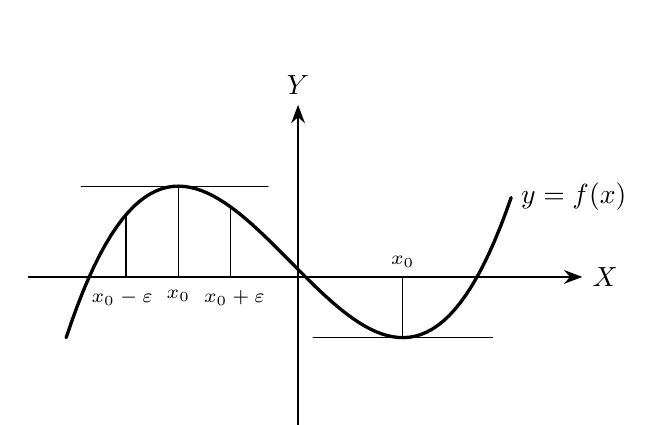
\begin{tikzpicture}[>=Stealth, scale=0.95, line cap=round, line join=round]
  \draw[->, thick] (-3.6, 0) -- (3.8, 0) node[right] {$X$};
  \draw[->, thick] (0, -2.1) -- (0, 2.3) node[above] {$Y$};

  % Explicit cubic with local max at x = -1.6 (y=1.214), local min at x = 1.4 (y=-0.811)
  % Left root at x ~ -2.79, clearing x_0-\varepsilon completely
  \draw[very thick, domain=-3.10:2.85, samples=80]
    plot (\x, {0.15*\x*\x*\x + 0.045*\x*\x - 1.008*\x + 0.10});
  \node[right] at (2.85, 1.07) {$y=f(x)$};

  % Horizontal tangents at extrema (matching original p.110)
  \draw[thin] (-2.9, 1.214) -- (-0.4, 1.214);
  \draw[thin] (0.2, -0.811) -- (2.6, -0.811);

  % Three vertical lines around local max x0 = -1.6 with generous spacing
  % f(-2.30) = 0.831, f(-1.60) = 1.214, f(-0.90) = 0.934
  \draw[thin] (-2.30, 0) -- (-2.30, 0.831);
  \draw[thin] (-1.60, 0) -- (-1.60, 1.214);
  \draw[thin] (-0.90, 0) -- (-0.90, 0.934);
  \node[below, font=\scriptsize] at (-2.35, -0.05) {$x_0-\varepsilon$};
  \node[below, font=\scriptsize] at (-1.60, -0.05) {$x_0$};
  \node[below, font=\scriptsize] at (-0.85, -0.05) {$x_0+\varepsilon$};

  % Vertical line at local min x0 = 1.4
  \draw[thin] (1.4, 0) node[above, font=\scriptsize] {$x_0$} -- (1.4, -0.811);
\end{tikzpicture}
\end{figure}

從上圖可看出所謂的極大、極小值，只是跟該函數在該點近傍的函數值做比較而已。它不一定是整個定義區間中的最大值或是最小值。我們可作出一個函數的圖形有二個以上的極大值：

\begin{figure}[H]
\centering
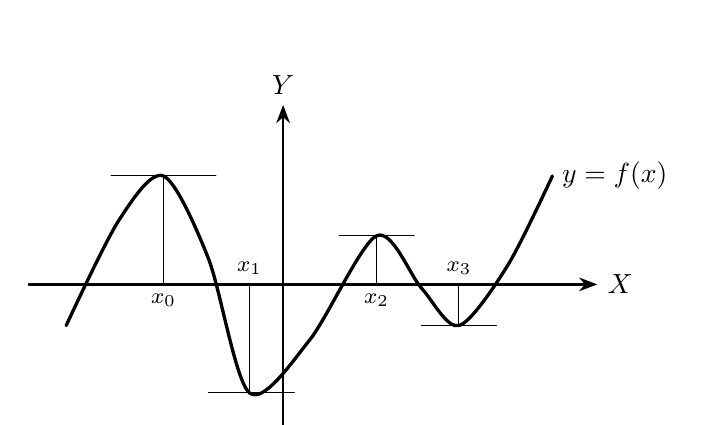
\begin{tikzpicture}[>=Stealth, scale=0.95, line cap=round, line join=round]
  \draw[->, thick] (-3.4, 0) -- (4.2, 0) node[right] {$X$};
  \draw[->, thick] (0, -2.0) -- (0, 2.4) node[above] {$Y$};

  % Smooth curve with 4 extrema: x0=-1.6 (max 1.4), x1=-0.45 (min -1.45), x2=1.25 (max 0.65), x3=2.35 (min -0.55)
  \draw[very thick, smooth] plot coordinates {
    (-2.9, -0.55) (-2.2, 0.85) (-1.6, 1.45) (-1.0, 0.35) (-0.45, -1.45)
    (0.35, -0.75) (1.25, 0.65) (1.85, -0.05) (2.35, -0.55) (3.0, 0.25) (3.6, 1.45)
  };
  \node[right] at (3.6, 1.45) {$y=f(x)$};

  % Horizontal tangent segments and vertical lines (matching original p.111)
  \draw[thin] (-2.3, 1.45) -- (-0.9, 1.45);
  \draw[thin] (-1.0, -1.45) -- (0.15, -1.45);
  \draw[thin] (0.75, 0.65) -- (1.75, 0.65);
  \draw[thin] (1.85, -0.55) -- (2.85, -0.55);

  \draw[thin] (-1.6, 0) node[below, font=\footnotesize] {$x_0$} -- (-1.6, 1.45);
  \draw[thin] (-0.45, 0) node[above, font=\footnotesize] {$x_1$} -- (-0.45, -1.45);
  \draw[thin] (1.25, 0) node[below, font=\footnotesize] {$x_2$} -- (1.25, 0.65);
  \draw[thin] (2.35, 0) node[above, font=\footnotesize] {$x_3$} -- (2.35, -0.55);
\end{tikzpicture}
\end{figure}

函數 $f(x)$ 在 $x_0, x_2$ 有極大值，但 $f(x_0) > f(x_2)$。

回頭再來看看函數 $f(x)$ 的泰勒展開式：
\begin{align*}
f(x+h) - f(x) &= f'(x)h + f''(x)\dfrac{h^2}{2!} + f'''(x)\dfrac{h^3}{3!} + \dots + f^{(n)}(x)\dfrac{h^n}{n!} \\
&= f'(x)h + h^2 \left( f''(x)\dfrac{1}{2!} + f'''(x)\dfrac{h}{3!} + \dots + f^{(n)}(x)\dfrac{h^{n-2}}{n!} \right)
\end{align*}
如果 $f(x)$ 的第一階導函數 $f'(x)$ 在某點 $x_0$ 取得 0 值，即 $f'(x_0)=0$ 則得
\begin{equation}
f(x_0+h) - f(x_0) = h^2 \left[ f''(x_0)\dfrac{1}{2!} + f'''(x_0)\dfrac{h}{3!} + \dots + f^{(n)}(x_0)\dfrac{h^{n-2}}{n!} \right] \label{eq:b6s-2-4-extrema-1}
\end{equation}
當 $h$ 在很小很小的範圍內變動時，右邊有含 $h$ 的項數（不管 $f^{(i)}(x_0)$ 為正或負）皆為很小，因此 \eqref{eq:b6s-2-4-extrema-1} 式中右邊為正或負，完全取定於 $f''(x_0)$ 為正或為負。如 $f''(x_0)$ 為正，則對任意小數 $h, f(x_0+h)-f(x_0) \ge 0$ 即 $f(x)$ 在 $x_0$ 有極小值；如果 $f''(x_0)$ 為負，則對任意小數 $h, f(x_0+h)-f(x_0) \le 0$ 即 $f(x)$ 在 $x_0$ 有極大值。因此，我們可得下面的定理：

\begin{theorem}[極值判別法]\label{thm:b6s-2-extrema}
如果多項式函數 $f(x)$，對於一點 $x_0$，有
\[ \begin{cases} f'(x_0) = 0 \\ f''(x_0) < 0 \end{cases} \implies f(x) \text{ 在 } x_0 \text{ 有極大值} \]
如果
\[ \begin{cases} f'(x_0) = 0 \\ f''(x_0) > 0 \end{cases} \implies f(x) \text{ 在 } x_0 \text{ 有極小值} \]
\end{theorem}

\begin{example}\label{ex:b6s-2-22}
令 $f(x)$ 為二次函數求極大、極小值。
\end{example}

\paragraph{【解】}
$f(x) = a_2 x^2 + a_1 x + a_0$
$f'(x) = 2a_2 x + a_1$
$f''(x) = 2a_2$
令 $f'(x) = 2a_2 x + a_1 = 0 \implies x = \dfrac{-a_1}{2a_2}$。
$f(x)$ 在 $x_0 = \dfrac{-a_1}{2a_2}$ 取極大或極小值。
如果 $a_2 > 0$，$f(x)$ 在 $x_0$ 有極小值，極小值為 $f\left(\dfrac{-a_1}{2a_2}\right)$。
如果 $a_2 < 0$，$f(x)$ 在 $x_0$ 有極大值，極大值為 $f\left(\dfrac{-a_1}{2a_2}\right)$。\hfill$\#$

\begin{example}\label{ex:b6s-2-23}
$f(x)=x^2+2x+2$，求 $f(x)$ 的極大，極小值。
\end{example}

\paragraph{【解】}
$f'(x)=2x+2$。故 $2x+2=0 \implies x=-1$。
$f(x)$ 在 $x=-1$ 得極小值，極小值為 $f(-1)=1+2(-1)+2=1$。
各位很容易用配方法知
\[ f(x) = (x+1)^2+1 \ge 1 \qquad \text{當 } x=-1 \text{ 時 } f(x) \text{ 最小}=1 \]\hfill$\#$

\subsubsection*{作業 14}\label{hw:b6s-2-14}
求 $f(x)=x^3+3x^2-x-3$ 之極大、極小值。

\subsubsection*{習題 II-4}\label{sec:b6s-ex2-4}

\begin{enumerate}[label=\arabic*., leftmargin=2em]
  \item 試求下列各多項式的導函數：
  \begin{multicols}{2}
  \begin{enumerate}[label=(\roman*)]
    \item $x^4-3x^2+5$
    \item $x^5-3x^4+5x^2+7$
    \item $(x-1)^3(x+2)^2$
    \item $(x^2+1)^2(x-5)^3$
  \end{enumerate}
  \end{multicols}

  \item 試求下列各多項式的導數：
  \begin{enumerate}[label=(\roman*)]
    \item $f(x)=x^3-4x^2+5$ 求 $f'(1), f''(0), f'''(3), f^{(4)}(0)$。
    \item $f(x)=x^3(x^3-3x^2+6x+4)$，求 $f'(0), f''(0), f'''(0)$。
  \end{enumerate}

  \item 試把 $x^3+4x^2+5x-7$ 展開為 $x-2$ 的泰勒展開式。

  \item 給定 $f(x)=4x^3-3x^2-7x+5$
  \begin{enumerate}[label=(\roman*)]
    \item 試求 $f(x)$ 在 $x=-3$ 的泰勒展開式。
    \item 求 $f(-3.01)$ 至小數第 3 位。
  \end{enumerate}

  \item 已知 $f(x)=x^4+x^3+ax^2+bx-2=0$ 有 $x=1$ 的二重根，求 $a, b$。

  \item 已知 $f(x)=x^5-5x^3+5x+2=0$ 有重根，試解之。

  \item 已知下列各方程式有重根，試解之：
  \begin{enumerate}[label=(\roman*)]
    \item $x^4-6x^3+13x^2-12x+4=0$
    \item $x^4-x^3-3x^2+5x-2=0$
    \item $x^4+4x^3+10x^2+12x+9=0$
  \end{enumerate}

  \item 試問下列各方程式有重根時 $a$ 值如何？
  \begin{enumerate}[label=(\roman*)]
    \item $f(x)=x^3-3x+a=0$
    \item $f(x)=3x^4+4x^3-6x^2-12x+a=0$
  \end{enumerate}

  \item 試求下列各函數的極大、極小值：
  \begin{enumerate}[label=(\roman*)]
    \item $x^3-3x^2+4$
    \item $x^2(x+4)^2$
    \item $2x^3+x^2-8x+2$
  \end{enumerate}
\end{enumerate}

\subsection{*三次方程式、四次方程式的解法}\label{sec:b6s-2-5}
\resetsectcounters

任意實係數一次方程式 $ax+b=0$ 之解為 $x=-\dfrac{b}{a}$，任意實係數二次方程式 $ax^2+bx+c=0$ 之解為 $x=\dfrac{-b \pm \sqrt{b^2-4ac}}{2a}$，那麼是否有一公式可以將任意三次方程式 $a_3 x^3 + a_2 x^2 + a_1 x + a_0 = 0$ 解出來呢？

在 16 世紀，對於三次方程式已有解法，通稱\textbf{卡丹解法}，四次方程式亦有公式解，至於五次方程式以上，已證出：

\begin{theorem}\label{thm:b6s-2-abel-ruffini}
若 $n$ 為大於 4 之正整數，則必有不能開方解出之 $n$ 次方程式存在。
\end{theorem}

探究未知是人類求生存必然的活動，歸納已知的事實推廣到一般現象是我們習於操作的，但什麼樣的事實可以歸納？例如對一元的一次、二次、三次、四次方程式，若都可求得公式解，是否對五次以上亦做得到？利用代數方法已證明這是不可能的了。因為證明中用到較深一點的數學工具，證明的方法未能普遍授於眾人，這件不可能的事實到今天還不為眾所周知。這樣的事正像到今天還有不知多少人耗費他們的精力求做柏拉圖提出的名題，以直尺（無刻度的）及圓規三等分一個角一樣。並不是角不能三等分，這問題與所用的工具有關，工匠早就知道利用等分線段的方法準確地三等分一個角，而 Euclid 也早就揚棄柏拉圖的限制做出三等分來，但若要受柏拉圖所加的限制便是絕對做不到。它之不可能可以由方程式論的觀點來看，你若難以相信這件事，就請你在嘗試去做之前，花點精力認識一下這件事的證明過程，而如果你實在有需要三等分一個角，何不掙開柏拉圖給的限制，採用便利的工具？我們不必再為這個問題鑽牛角尖，而用我們的精力去尋求可能存在的另一些真理。

\subsubsection*{甲、一元三次方程式的解法}\label{subsec:b6s-2-5-a}

設實係數三次方程式為
\begin{equation}
a_3 x^3 + a_2 x^2 + a_1 x + a_0 = 0 \label{eq:b6s-2-5-1}
\end{equation}
以 $a_3$ 遍除各項得
\begin{equation}
x^3 + \dfrac{a_2}{a_3}x^2 + \dfrac{a_1}{a_3}x + \dfrac{a_0}{a_3} = 0 \label{eq:b6s-2-5-2}
\end{equation}
(1) 與 (2) 有相同的根，故我們只考慮這樣的三次式
\begin{equation}
x^3 + bx^2 + cx + d = 0 \label{eq:b6s-2-5-3}
\end{equation}
以 $x = z - \dfrac{b}{3}$ 代入，可得一新方程式
\begin{equation}
z^3 + pz + q = 0 \label{eq:b6s-2-5-4}
\end{equation}
其中消去二次項，(4) 式中諸根減 $\dfrac{b}{3}$ 得 (3) 式中諸根，因此吾人只需解 (4) 式，令
\begin{equation}
z = u - \dfrac{p}{3u} \label{eq:b6s-2-5-5}
\end{equation}
代入 (4)
\[ \left( u - \dfrac{p}{3u} \right)^3 + p\left( u - \dfrac{p}{3u} \right) + q = 0 \]
整理之，得
\begin{equation}
u^3 - \dfrac{p^3}{27u^3} + q = 0 \label{eq:b6s-2-5-6}
\end{equation}
即
\begin{equation}
(u^3)^2 + qu^3 - \dfrac{p^3}{27} = 0 \label{eq:b6s-2-5-7}
\end{equation}
視此為 $u^3$ 的二次式，利用公式得
\begin{align}
u^3 &= \dfrac{-q + \sqrt{q^2 + 4\frac{p^3}{27}}}{2} = -\dfrac{q}{2} + \sqrt{\dfrac{q^2}{4} + \dfrac{p^3}{27}} \label{eq:b6s-2-5-8} \\
u^3 &= -\dfrac{q}{2} - \sqrt{\dfrac{q^2}{4} + \dfrac{p^3}{27}} \label{eq:b6s-2-5-9}
\end{align}
令
\begin{align*}
\alpha &= \sqrt[3]{-\dfrac{q}{2} + \sqrt{\dfrac{q^2}{4} + \dfrac{p^3}{27}}} \tag{I} \\
\beta &= \sqrt[3]{-\dfrac{q}{2} - \sqrt{\dfrac{q^2}{4} + \dfrac{p^3}{27}}} \tag{II}
\end{align*}
設 $\omega$ 為 $x^3=1$ 之複數根，$1+\omega+\omega^2=0$。\\
得 \eqref{eq:b6s-2-5-8} 中 $u$ 有三解：$\alpha, \alpha\omega, \alpha\omega^2$。\\
\eqref{eq:b6s-2-5-9} 中 $u$ 有三解：$\beta, \beta\omega, \beta\omega^2$。\\
代入 \eqref{eq:b6s-2-5-5} 得
\[ z = \alpha+\beta, \quad \omega\alpha+\omega^2\beta, \quad \omega^2\alpha+\omega\beta \]
此即為三次式的三根。

\begin{example}\label{ex:b6s-2-24}
試解 $x^3-6x^2+6x-2=0$。
\end{example}

\paragraph{【解】}
令 $y=x-2$ 代入得 $y^3-6y-6=0$ 其中 $p=-6, q=-6$。
代入公式 (I), (II) 得
\[ \alpha = \sqrt[3]{4}, \quad \beta = \sqrt[3]{2} \]
所以
\[ y = \sqrt[3]{4}+\sqrt[3]{2}, \quad \sqrt[3]{4}\omega+\sqrt[3]{2}\omega^2, \quad \sqrt[3]{4}\omega^2+\sqrt[3]{2}\omega \]
故原方程式之根為 $2+\sqrt[3]{4}+\sqrt[3]{2}, 2+\sqrt[3]{4}\omega+\sqrt[3]{2}\omega^2, 2+\sqrt[3]{4}\omega^2+\sqrt[3]{2}\omega$。\hfill$\#$

\subsubsection*{乙、一元四次方程式的解法}\label{subsec:b6s-2-5-b}

設實係數一元四次方程式為
\begin{equation}
x^4 + ax^3 + bx^2 + cx + d = 0 \label{eq:b6s-2-5-10}
\end{equation}
於 \eqref{eq:b6s-2-5-10} 左右兩端各加 $(px+q)^2$，得
\begin{equation}
x^4 + ax^3 + bx^2 + cx + d + (px+q)^2 = (px+q)^2 \label{eq:b6s-2-5-11}
\end{equation}
假設 \eqref{eq:b6s-2-5-11} 左邊為完全平方 $= \left(x^2 + \dfrac{a}{2}x + k\right)^2$。展開比較係數得
\begin{equation}
2k + \dfrac{a^2}{4} = b + p^2, \quad ak = c + 2pq, \quad k^2 = d + q^2 \label{eq:b6s-2-5-12}
\end{equation}
故
\[ p^2 = 2k + \dfrac{a^2}{4} - b, \quad q^2 = k^2 - d, \quad 2pq = ak - c \]
得
\[ 4(k^2-d)\left(2k+\dfrac{a^2}{4}-b\right) = (ak-c)^2 \]
此為 $k$ 的三次方程式：
\[ 8k^3 - 4bk^2 - 2(ac-4d)k + 4bd - a^2d - c^2 = 0 \]
求得實數解 $k$ 後，利用 \eqref{eq:b6s-2-5-12} 決定 $p, q$ 值。又由 \eqref{eq:b6s-2-5-10}, \eqref{eq:b6s-2-5-11} 知
\[ \left(x^2 + \dfrac{a}{2}x + k\right)^2 = (px+q)^2 \]
故原方程式可分解為二個二次方程式，為
\begin{align*}
x^2 + \dfrac{a}{2}x + k - px - q &= 0 \\
x^2 + \dfrac{a}{2}x + k + px + q &= 0
\end{align*}
此二方程之解，即為原方程式之解。

\begin{example}\label{ex:b6s-2-25}
試解四次方程式
\[ x^4 + 8x^3 + 12x^2 - 11x + 2 = 0 \]
\end{example}

\paragraph{【解】}
\setcounter{equation}{0}%
於原方程式兩端各加以 $(px+q)^2$ 得
\begin{equation}
x^4 + 8x^3 + 12x^2 - 11x + 2 + (px+q)^2 = (px+q)^2 \label{eq:b6s-2-5-ex2-1}
\end{equation}
假設
\begin{equation}
x^4 + 8x^3 + 12x^2 - 11x + 2 + p^2x^2 + 2pqx + q^2 = (x^2+4x+k)^2 \label{eq:b6s-2-5-ex2-2}
\end{equation}
比較 \eqref{eq:b6s-2-5-ex2-2} 式左右兩端係數，得
\begin{equation}
16 + 2k = 12 + p^2, \quad 8k = 2pq - 11, \quad k^2 = 2 + q^2 \label{eq:b6s-2-5-ex2-3}
\end{equation}
消去 $p, q$ 得 $k$ 之三次方程式：
\begin{equation}
8k^3 - 48k^2 - 192k - 153 = 0 \label{eq:b6s-2-5-ex2-4}
\end{equation}
利用公式解 (4)，得 $k$ 之實根為 $k = -\dfrac{3}{2}$。代入 \eqref{eq:b6s-2-5-ex2-3} 得
\[ p = 1, \quad q = -\dfrac{1}{2} \]
以 $k, p, q$ 之值代入 \eqref{eq:b6s-2-5-ex2-1}, \eqref{eq:b6s-2-5-ex2-2} 得
\[ \left(x^2+4x-\dfrac{3}{2}\right)^2 = \left(x-\dfrac{1}{2}\right)^2 \]
故得
\[ \begin{cases}
x^2 + 3x - 1 = 0 \\
x^2 + 5x - 2 = 0
\end{cases} \]
解之得原方程式四根為
\[ \dfrac{-3 \pm \sqrt{13}}{2} \quad \text{及} \quad \dfrac{-5 \pm \sqrt{33}}{2} \]\hfill$\#$

\subsubsection*{習題 II-5}\label{sec:b6s-ex2-5}

\begin{enumerate}[label=\arabic*., leftmargin=2em]
  \item 試解 $x^3-6x+4=0$。
  \item 試解 $x^3-3x^2-3x-1=0$。
  \item 試解 $x^3-2x^2+1=0$。
  \item 試解 $x^3-12x+65=0$。
  \item 試解 $x^3-9x+28=0$。
  \item 設 $x^3+px+r=0$ 的三根皆為實根，試證 $p, r$ 為負，且 $-4p^3r > 27r$\phantomsection\label{note:b6s-ch2-p117-cubic-ineq}\footnote{【原書註記】：依判別式條件，原書所列不等式 $-4p^3 > 27r^2$ 印損為 $-4p^3r > 27r$。}。
  \item 試解下列四次方程式：
  \begin{multicols}{2}
  \begin{enumerate}[label=(\roman*)]
    \item $x^4+2x^3+14x+15=0$
    \item $x^4-12x-5=0$
    \item $x^4-12x^2+24x+140=0$
    \item $x^4-14x^3+71x^2-154x+120=0$
    \item $x^4-2x^3-5x^2+10x-3=0$
    \item $x^4+8x^3+22x^2+32x+21=0$
  \end{enumerate}
  \end{multicols}
\end{enumerate}

\phantomsection
\subsection*{附錄 III\quad 結式判別式與史篤姆定理}\label{sec:b6s-app3}
\addcontentsline{toc}{subsection}{\texorpdfstring{附錄 III\quad 結式判別式與史篤姆定理}{附錄 III 結式判別式與史篤姆定理}}
\resetsectcounters

\subsubsection*{1. 結式}\label{subsec:b6s-app3-1}

設二個一元方程式為
\begin{align}
f(x) &= a_0 x^3 + a_1 x^2 + a_2 x + a_3 = 0 \label{eq:b6s-app3-1} \\
g(x) &= b_0 x^2 + b_1 x + b_2 = 0 \label{eq:b6s-app3-2}
\end{align}
\eqref{eq:b6s-app3-1} 式分別乘以 $x, 1$，\eqref{eq:b6s-app3-2} 式分別乘以 $x^2, x, 1$ 得
\begin{equation}
\left\{\begin{aligned}
a_0 x^4 + a_1 x^3 + a_2 x^2 + a_3 x &= 0 \\
a_1 x^3 + a_1 x^2 + a_2 x + a_3 &= 0 \\
b_0 x^4 + b_1 x^3 + b_2 x^2 &= 0 \\
b_0 x^3 + b_1 x^2 + b_2 x &= 0 \\
b_0 x^2 + b_1 x + b_2 &= 0
\end{aligned}\right. \label{eq:b6s-app3-6}
\end{equation}
把 (3) 式看做 $x^4, x^3, x^2, x, 1$ 的五元一次聯立方程式，如果 (3) 有共同解，由克萊瑪法則知其係數行列式
\[ D = \begin{vmatrix}
a_0 & a_1 & a_2 & a_3 & 0 \\
0 & a_0 & a_1 & a_2 & a_3 \\
b_0 & b_1 & b_2 & 0 & 0 \\
0 & b_0 & b_1 & b_2 & 0 \\
0 & 0 & b_0 & b_1 & b_2
\end{vmatrix} = 0 \]
反之如果 $D=0$，由行列式的運算，得
\[ 0 = \begin{vmatrix}
a_0 & a_1 & a_2 & a_3 & x(a_0 x^3 + a_1 x^2 + a_2 x + a_3) \\
0 & a_0 & a_1 & a_2 & a_0 x^3 + a_1 x^2 + a_2 x + a_3 \\
b_0 & b_1 & b_2 & 0 & x^2(b_0 x^2 + b_1 x + b_2) \\
0 & b_0 & b_1 & b_2 & x(b_0 x^2 + b_1 x + b_2) \\
0 & 0 & b_0 & b_1 & b_0 x^2 + b_1 x + b_2
\end{vmatrix} \]
設 $\alpha_1, \alpha_2, \alpha_3, \alpha_4, \alpha_5$ 分別為 $D$ 中第五列的餘因式，則得
\begin{equation}
0 \equiv D \equiv (\alpha_1 x + \alpha_2) f(x) + (\alpha_3 x^2 + \alpha_4 x + \alpha_5) g(x) \label{eq:b6s-app3-4}
\end{equation}
由 (4) 式知，如果 $(x-B)$ 為 $f(x)$ 的一個因式，則 $x-B$ 必為 $(\alpha_3 x^2 + \alpha_4 x + \alpha_5) g(x)$ 的因式。因 $f(x)=0$ 有三個根，而 $\alpha_3 x^2 + \alpha_4 x + \alpha_5 = 0$ 為二次方程式，故 $f(x)=0$ 與 $g(x)=0$ 必共根。

\begin{definition}\label{def:b6s-app3-resultant}
設 $f(x) = a_0 x^n + a_1 x^{n-1} + \dots + a_n = 0, g(x) = b_0 x^m + b_1 x^{m-1} + \dots + b_m = 0$ 分別為 $n, m$ 次方程式，則它們的\textbf{結式} $D(f, g)$ 為 $m+n$ 階行列式：
\[ D(f, g) = \begin{vmatrix}
a_0 & a_1 & a_2 & \dots & a_n & 0 & 0 & \dots & 0 \\
0 & a_0 & a_1 & \dots & a_{n-1} & a_n & 0 & \dots & 0 \\
0 & 0 & \dots & \dots & \dots & \dots & \dots & \dots & \dots \\
0 & 0 & \dots & 0 & a_0 & a_1 & a_2 & \dots & a_n \\
b_0 & b_1 & \dots & \dots & \dots & b_m & 0 & \dots & 0 \\
0 & b_0 & b_1 & \dots & \dots & \dots & b_{m-1} & b_m & 0 \\
\dots & \dots & \dots & \dots & \dots & \dots & \dots & \dots & \dots \\
0 & \dots & 0 & b_0 & b_1 & \dots & \dots & \dots & b_m
\end{vmatrix} \]
\end{definition}

從上述的討論可得：

\begin{theorem}\label{thm:b6s-app3-resultant-roots}
設 $f(x) = a_0 x^n + \dots + a_n = 0, g(x) = b_0 x^m + \dots + b_m = 0$ 分別為 $n, m$ 次方程式。則 $f(x)=0, g(x)=0$ 有共根之充要條件為 $D(f, g) = 0$。
\end{theorem}

\begin{example}\label{ex:b6s-app3-1}
試證 $x^2+3x+2=0$ 與 $x+1=0$ 有共根。
\end{example}

\paragraph{【解】}
$D = \begin{vmatrix} 1 & 3 & 2 \\ 1 & 1 & 0 \\ 0 & 1 & 1 \end{vmatrix} = 1 + 2 - 3 = 0$。故 $x^2+3x+2=0$ 與 $x+1=0$ 有共根。\\
事實上我們很容易看出 $x^2+3x+2 = (x+1)(x+2)$ 有一根為 $-1$。\hfill$\#$

\subsubsection*{2. 判別式}\label{subsec:b6s-app3-2}

\begin{definition}\label{def:b6s-app3-discriminant}
給一方程式 $f(x) = a_0 x^n + a_1 x^{n-1} + \dots + a_n = 0$ ($a_0 \ne 0$)，$D(f, f')/a_0$ 稱為 $f(x)$ 的\textbf{判別式}。
\end{definition}

我們從上節中知 $f(x)=0$ 與 $f'(x)=0$ 有共根之充要條件是 $D(f, f') = 0$，因此我們能從 $D(f) = D(f, f')/a_0$ 中知 $f(x)=0$ 有沒有重根。

\begin{example}\label{ex:b6s-app3-2}
設二次方程式為 $f(x)=a_0 x^2 + a_1 x + a_2 = 0$，則 $f'(x)=2a_0 x + a_1$。
\end{example}

得
\begin{align*}
D &= \dfrac{1}{a_0} D(f, f') = \dfrac{1}{a_0} \begin{vmatrix}
a_0 & a_1 & a_2 \\
2a_0 & a_1 & 0 \\
0 & 2a_0 & a_1
\end{vmatrix} \\
&= \dfrac{1}{a_0}(a_0 a_1^2 + 4a_0^2 a_2 - 2a_0 a_1^2) = -(a_1^2 - 4a_0 a_2)
\end{align*}
故 $f(x)=0$ 有重根之充要條件為 $a_1^2 - 4a_0 a_2 = 0$。\hfill$\#$

一般的判別式有下列定理：

\begin{theorem}\label{thm:b6s-app3-disc-roots}
設 $\beta_1, \beta_2, \dots, \beta_n$ 為 $f(x) = a_0 x^n + \dots + a_n = 0$ 的 $n$ 個根，則 $f(x)=0$ 的判別式為
\[ D(f) = C(\beta_1-\beta_2)^2 \dots (\beta_1-\beta_n)^2 \dots (\beta_i-\beta_j)^2 \dots (\beta_{n-1}-\beta_n)^2 \]
即 $D(f) = C \prod_{i<j} (\beta_i-\beta_j)^2$，$C$ 為常數。
\end{theorem}

\subsubsection*{3. 史篤姆 (Sturm's) 定理}\label{subsec:b6s-app3-3}

設一方程式 $f(x)=0$ 無重根，$f_1(x)=f'(x)$ 為 $f(x)$ 的第一階導函數。令
\begin{equation}
f(x) \equiv q_1 f_1(x) - f_2(x) \label{eq:b6s-app3-sturm-1}
\end{equation}
$q_1(x)$ 為 $f(x)$ 被 $f_1(x)$ 除的商，而 $-f_2(x)$ 為其餘式，同理令
\begin{align}
f_1(x) &\equiv q_2 f_2(x) - f_3(x) \label{eq:b6s-app3-sturm-2} \\
f_{m-2}(x) &\equiv q_{m-1} f_{m-1}(x) - f_m(x) \label{eq:b6s-app3-sturm-3}
\end{align}
而設 $-f_m(x)$ 為常數。因為 $f(x)$ 無重根故這樣輾轉相除的最後項 $f_m(x)$ 不等於 0。這樣的一組函數
\[ f(x), f_1(x), f_2(x), \dots, f_m(x) \]
稱為 $f(x)$ 的 \textbf{Sturm's 函數}。

設取任二數 $a, b$ ($a < b$) 考慮下列數列：
\begin{align}
f(a), f_1(a), f_2(a), \dots, f_m(a) \label{eq:b6s-app3-sturm-a} \\
f(b), f_1(b), f_2(b), \dots, f_m(b) \label{eq:b6s-app3-sturm-b}
\end{align}
設 \eqref{eq:b6s-app3-sturm-a} 中相鄰二數變號的個數為 $n$，\eqref{eq:b6s-app3-sturm-b} 中相鄰二數變號的個數為 $m$，則

\begin{theorem}[Sturm 定理]\label{thm:b6s-app3-sturm}
設 $f(x)=0$，有 $l$ 個根落在 $[a, b]$ 中，則
\[ l = n - m \]
（定理的證明從略）
\end{theorem}

\begin{example}\label{ex:b6s-app3-3}
$f(x) = x^3 + 3x^2 - 4x + 1 = 0$
\end{example}

\paragraph{【解】}
$f'(x) = f_1(x) = 3x^2 + 6x - 4$。用輾轉相除法得 $f(x)$ 的 Sturm 函數為
\begin{align*}
f(x) &= x^3 + 3x^2 - 4x + 1 \\
f_1(x) &= 3x^2 + 6x - 4 \\
f_2(x) &= 2x - 1 \\
f_3(x) &= 1
\end{align*}
(1)
\begin{center}
\renewcommand{\arraystretch}{1.3}
\begin{tabular}{c|c|c|c|c|l}
& $f(x)$ & $f_1(x)$ & $f_2(x)$ & $f_3(x)$ & \\
\hline
$x = -\infty$ & $-$ & $+$ & $-$ & $+$ & 三個變號 \\
$x = 0$       & $+$ & $-$ & $-$ & $+$ & 二個變號 \\
$x = \infty$  & $+$ & $+$ & $+$ & $+$ & 無變號
\end{tabular}
\end{center}
故知 $(-\infty, 0]$ 中有一根，$[0, \infty)$ 有二根。

(2)
\begin{center}
\renewcommand{\arraystretch}{1.3}
\begin{tabular}{c|c|c|c|c|l}
& $f(x)$ & $f_1(x)$ & $f_2(x)$ & $f_3(x)$ & \\
\hline
$x = 0$ & $+$ & $-$ & $-$ & $+$ & 二個變號 \\
$x = 1$ & $+$ & $+$ & $+$ & $+$ & 無變號
\end{tabular}
\end{center}
故知 $f(x)$ 的二正根落在 $[0, 1]$ 間。\hfill$\#$
 % 第二章 方程式論
% !TeX root = Chapter3_main.tex
% =========================================================================
% 《高中數學實驗教材》第六冊（社會組）
% 第三章 高中數學教材的回顧
% =========================================================================
\section{高中數學教材的回顧}\label{sec:b6s-ch3}\label{sec:b6s-3}

\begin{center}
\begin{minipage}{0.75\textwidth}
\begin{itemize}[leftmargin=3em, itemsep=0.3em]
  \item[§ III-1] \textbf{例說逼近}
  \item[§ III-2] \textbf{進一步的基本模型}
  \begin{itemize}[leftmargin=2em, itemsep=0.2em]
    \item[甲、] 有理函數
    \item[乙、] 三角函數
    \item[丙、] 指數與對數函數
  \end{itemize}
  \item[§ III-3] \textbf{以「逼近」觀點看課程內容}
  \begin{itemize}[leftmargin=2em, itemsep=0.2em]
    \item[(A)] 數量化與數
    \item[(B)] 單變數函數模型
    \item[(C)] 多變數函數及其基本模型：線性映射與二次式函數
    \item[(D)] 機率與統計
  \end{itemize}
  \item[§ III-4] \textbf{以「轉化」觀點看課程內容}
  \begin{itemize}[leftmargin=2em, itemsep=0.2em]
    \item[(E)] 轉化
    \item[(F)] 兩個系統轉化
    \item[(G)] 進一步的轉化
  \end{itemize}
  \item[§ III-5] \textbf{尾語}
\end{itemize}
\end{minipage}
\end{center}

\begin{center}
$* \qquad * \qquad * \qquad * \qquad *$
\end{center}

\subsection{例說逼近}\label{sec:b6s-3-1}

高中數學的教材主要是在「逼近」與「轉化」兩種觀點之下交迭推進的。

「逼近」是人類設法要描寫或了解自然（或人文的）現象時，所產生及採用的一種過程：

換句話說，人類在對於較單純的自然現象徹底了解後，把它當作一種「模型」，例如速度 $a$ 一定時，位移 $S$ 與時間 $t$ 的關係，
\begin{equation}
S = at + b \qquad (\text{其中 } b \text{ 表 } t=0 \text{ 時已有的位移}) \label{eq:b6s-3-1}
\end{equation}
又例如圓面積 $A$ 與其半徑 $r$ 間的關係
\begin{equation}
A = \pi r^2 \label{eq:b6s-3-2}
\end{equation}
有了這些「模型」之後，對於一些複雜的實際現象，便將這些模型套上去，看看與實際現象的差距是否夠小？

像 \eqref{eq:b6s-3-1} 這種函數，經一般化後，寫成
\begin{equation}
y = a_1 x + a_0 \qquad (\text{其中 } a_1, a_0 \text{ 皆為常數}) \label{eq:b6s-3-3}
\end{equation}
稱為一次函數，而像 \eqref{eq:b6s-3-2} 這種函數，則可寫成
\begin{equation}
y = a_2 x^2 \qquad (\text{其中 } a_2 \text{ 為常數}) \label{eq:b6s-3-4}
\end{equation}
將 \eqref{eq:b6s-3-3}, \eqref{eq:b6s-3-4} 作和，得
\begin{equation}
y = a_2 x^2 + a_1 x + a_0 \label{eq:b6s-3-5}
\end{equation}
稱為一般的二次函數。

再把上述「逼近」的想法重述一番：

我們所謂的「現象」，常以「變量間的關係」這一面目出現，（例如上述 $S$ 與 $t$ 間或 $A$ 與 $r$ 間的關係）。這種「變量間的關係」中，最單純的，可以說是一次函數與二次函數，即
\[ y = a_2 x^2 + a_1 x + a_0 \qquad (\text{其中 } a_2 \text{ 可}=0, \text{可}\ne 0) \]
這種較單純的函數，便是我們的「模型」，以下我們舉例來看怎麼利用「模型」來逼近地描寫實際現象：

\begin{discussion}[複選題]\label{ex:b6s-3-1}\label{disc:b6s-3-1}
設有某廠商出售衣服，單件價格記為 $x$，其一星期銷售量記為 $y$，由一般常識知：$y$ 隨著 $x$ 而變，即價格 $x$ 越高，銷售量 $y$ 就越小\phantomsection\label{note:b6s-ch3-p124-sales}\footnote{【原書校訂】：原書此處印作「價格 $x$ 越高，銷售量 $y$ 就越大」，依經濟學常理及下文調查數據（$x=2$ 時 $y=9$，$x=5$ 時 $y=6$）為負相關，原書「越大」顯係誤植，茲予校訂為「越小」。}。表成函數符號，為 $y=f(x)$。今作一市場調查，得數據如下：
\[ \text{當 } x=2 \text{ 時 } y=9, \quad \text{又當 } x=5 \text{ 時 } y=6 \]
若假定 $y$ 為 $x$ 的一次函數，換句話說：
\[ y = f(x) = a_1 x + a_0 \]

\begin{enumerate}[label=(\Roman*), leftmargin=2.5em]
  \item 求一滿足上述數據的 $x, y$ 間的關係：
  \begin{multicols}{2}
  \begin{enumerate}[label=(\Alph*)]
    \item $y = x+7$
    \item $y = 2x+5$
    \item $y = 9$
    \item $y = \dfrac{1}{2}x + \dfrac{7}{2}$
    \item $y = -x+11$
  \end{enumerate}
  \end{multicols}
  請畫出此函數圖形（呈一直線），以便繼續討論：

  \item 根據上述結果來做一推測，欲使銷售量 $y$ 不少於 9.5，則
  \begin{enumerate}[label=(\Alph*)]
    \item 價格 $x$ 可訂為 3 而最高不能超過 3
    \item 價格 $x$ 可訂為 1.5 而最高不能超過 1.5
    \item 價格 $x$ 可訂為 0.5 而最高不能超過 0.5
    \item 價格 $x$ 低於 1.1 皆可
    \item 價格 $x$ 須在 2 到 4 之間
  \end{enumerate}

  如再作調查，增一新數據為：$x=4$ 時 $y=8$。這時，一次函數已不能滿足 $(x,y)=(2,9), (5,6), (4,8)$ 這三個數據（有時一次函數仍可滿足其他某些的三個數據）。

  現在我們要改用二次函數來估計 $y$ 與 $x$ 的關係，即使設 $y=a_2 x^2 + a_1 x + a_0$ 滿足上述三個數據。（亦即以拋物線代替上述的直線）。

  \item 這 $x$ 與 $y$ 間的關係應表為：
  \begin{enumerate}[label=(\Alph*)]
    \item $x^2 + 5x + y - 12 = 0$
    \item $x^2 + ax + by = 12;\ a+b=-3$
    \item $x^2 = -y+b;\ b>0$
    \item $x^2 + ax + by = c;\ a+b+c \ge 9$
    \item $y = -x+11$
  \end{enumerate}

  這樣以二次函數來估計 $x$ 與 $y$ 的關係，理論上應比利用一次函數好，道理是它多符合了一個數據。

  \item 今據所得二次函數的估計，價格 $x$ 為 6 時預測銷售量 $y$
  \begin{multicols}{2}
  \begin{enumerate}[label=(\Alph*)]
    \item $4 \le y \le 6$
    \item $5 \le y \le 7$
    \item $2 \le y \le 4$
    \item $0 \le y \le 2$
    \item $y \le 3$
  \end{enumerate}
  \end{multicols}
\end{enumerate}

\paragraph{【答案】} (I) E, \ (II) B, D, \ (III) B, D, \ (IV) C, E
\end{discussion}

\subsubsection*{【論例 1 的分析】}

論例 1 中要知道的是單價 $x$ 如何影響銷售量 $y$？

開始我們根據兩週的調查數據，以一次函數
\[ y = -x+11 \]
的模型來逼近 $y$ 與 $x$ 間的實際關係，注意這個實際關係，若繪以函數圖形其曲折之形可能相當困難用式子描寫（見圖）。

\begin{center}
\renewcommand{\arraystretch}{1.2}
\begin{tabular}{|c|c|}
\hline
$x$ & $y$ \\ \hline
2 & 9 \\
5 & 6 \\ \hline
\end{tabular}
\end{center}

$y=-x+11$ 的模型，繪以函數圖形，呈一條直線，可以看到圖中原來曲折的實際曲線與這條作為模型的直線，雖有差距，但其趨勢似乎相近。

\begin{figure}[H]
\centering
\begin{tikzpicture}[>=Stealth, scale=1.0, line cap=round, line join=round]
  % 坐標軸
  \draw[->, thick] (-0.5, 0) -- (7.5, 0) node[right] {$X$} node[below=3pt, midway] {（單位價格）};
  \draw[->, thick] (0, -0.5) -- (0, 11) node[above] {$Y$};
  \node[left] at (-0.2, 5.5) {\rotatebox{90}{（一週銷售量）}};
  \node[below left] at (0, 0) {$O$};

  % 實際曲折數據曲線 (通過/靠近 (2,9), (4,8), (5,6))
  \draw[line width=1.5pt, smooth] plot coordinates {
    (1.5, 9.8) (1.8, 9.2) (2.0, 9.0) (2.5, 8.7) (3.0, 8.2) (3.5, 8.4)
    (4.0, 8.0) (4.5, 7.2) (4.8, 6.4) (5.0, 6.0) (5.3, 4.8) (5.8, 2.5) (6.2, 0.0)
  };

  % 一次函數直線模型 y = -x + 11
  \draw[thick, dash pattern=on 6pt off 3pt] (1.0, 10.0) -- (6.8, 4.2);

  % 標記點
  \filldraw[black] (2, 9) circle (2pt) node[above right] {$(2,9)$};
  \filldraw[black] (4, 8) circle (2pt) node[above right] {$(4,8)$};
  \filldraw[black] (5, 6) circle (2pt) node[above right] {$(5,6)$};
\end{tikzpicture}
\caption{一次函數模型 $y=-x+11$ 與實際銷售趨勢曲線之逼近比較}
\label{fig:b6s-3-linear-model}
\end{figure}

如果再多作一個星期的調查，得知
\[ \text{單價 } x=4 \text{ 時，銷售量 } y=8 \]
\begin{center}
\renewcommand{\arraystretch}{1.2}
\begin{tabular}{|c|c|}
\hline
$x$ & $y$ \\ \hline
2 & 9 \\
5 & 6 \\
4 & 8 \\ \hline
\end{tabular}
\end{center}

想根據這一新數據將上述的「模型」做得更精密，我們可取二次函數，而知要滿足三個星期的調查數據，這個二次函數應為
\[ y = -\dfrac{1}{2}x^2 + \dfrac{5}{2}x + 6 \]
其函數圖形為拋物線，在某一有效區段內，約略要比直線更逼近於代表實際現象的曲線。

換句話說，我們的模型從一次函數改進為二次函數，常常較能逼近實際現象。

\begin{figure}[H]
\centering
\begin{tikzpicture}[>=Stealth, scale=1.0, line cap=round, line join=round]
  % 坐標軸
  \draw[->, thick] (-0.5, 0) -- (7.5, 0) node[right] {$X$};
  \draw[->, thick] (0, -0.5) -- (0, 11) node[above] {$Y$};
  \node[below left] at (0, 0) {$O$};

  % 實際曲折數據曲線
  \draw[line width=1.5pt, smooth] plot coordinates {
    (1.5, 9.8) (1.8, 9.2) (2.0, 9.0) (2.5, 8.7) (3.0, 8.2) (3.5, 8.4)
    (4.0, 8.0) (4.5, 7.2) (4.8, 6.4) (5.0, 6.0) (5.3, 4.8) (5.8, 2.5) (6.2, 0.0)
  };

  % 二次函數拋物線模型 y = -0.5*x^2 + 2.5*x + 6
  \draw[thick, dash pattern=on 6pt off 3pt, domain=1.5:6.2, samples=60] 
    plot (\x, {-0.5*\x*\x + 2.5*\x + 6});

  % 標記點
  \filldraw[black] (2, 9) circle (2pt) node[above right] {$(2,9)$};
  \filldraw[black] (4, 8) circle (2pt) node[above right] {$(4,8)$};
  \filldraw[black] (5, 6) circle (2pt) node[above right] {$(5,6)$};
\end{tikzpicture}
\caption{二次函數拋物線模型 $y=-\frac{1}{2}x^2+\frac{5}{2}x+6$ 之精準逼近}
\label{fig:b6s-3-parabola-model}
\end{figure}

很自然地，問題繼續延伸：如果我們作了 $n+1$ 個星期的調查，該用什麼模型來逼近，才能滿足這 $n+1$ 次的調查數據？如此我們引進來一般的一 $n$ 次多項式函數：
\begin{equation}
y = a_n x^n + a_{n-1} x^{n-1} + \dots + a_1 x + a_0 \label{eq:b6s-3-6}
\end{equation}

總結一下這節的論點：

「自然或人文的現象常以函數的型態出現，這些函數一般時候相當複雜，我們處理的手法是這樣的：
\begin{enumerate}[label=\Roman*., leftmargin=2em]
  \item 建立基本模型。
  \item 以這些基本模型去推測實際現象。
\end{enumerate}
這節的例說，解釋了多項式函數
\begin{equation}
y = a_n x^n + a_{n-1} x^{n-1} + \dots + a_1 x + a_0 \label{eq:b6s-3-7}
\end{equation}
是一個值得採用的基本模型，也以函數的圖形顯示了「逼近描寫」的意義。

\subsection{進一步的基本模型}\label{sec:b6s-3-2}

\subsubsection*{甲、有理函數}\label{subsec:b6s-3-2-a}

牛頓的引力定律蘊涵下述的現象：

「一物體所受的地心引力 $y$ 與它到地心距離的平方 $x^2$ 成反比」

表成式子得：
\begin{equation}
y = \dfrac{k}{x^2} \qquad (k \text{ 與物體的位置無關}) \label{eq:b6s-3-8}
\end{equation}
這種函數並不是多項式函數，它是多項式函數 $x^2$ 的倒數，如果我們考慮兩個多項式函數 $P(x)$ 與 $Q(x)$ 的商，即
\begin{equation}
y = \dfrac{P(x)}{Q(x)} \label{eq:b6s-3-9}
\end{equation}
則 \eqref{eq:b6s-3-9} 式顯然概括了多項式函數 \eqref{eq:b6s-3-7}（此時取 $Q(x)\equiv 1$）與引力現象 \eqref{eq:b6s-3-8}（此時取 $P(x)\equiv k, Q(x)\equiv x^2$）。

\eqref{eq:b6s-3-9} 式是進一步的代數基本模型，稱為\textbf{有理函數}。

\subsubsection*{乙、三角函數}\label{subsec:b6s-3-2-b}

「波動」在自然界到處出現，從彈簧振動到水波，音波、光波、電磁波，都有一個共同的「和諧」的通性。

代數學基本定理（第六冊、第二章）告訴我們多項式函數，（甚至有理函數）相應的方程式最多只能有有限多個根，但波動可延伸成無限次的反覆（即週期性），故上述的代數基本模型無法描寫波動現象。

三角函數
\begin{equation}
y = \sin x \quad \text{或} \quad \cos x \quad \text{等} \label{eq:b6s-3-10}
\end{equation}
之所以值得討論，除為了三角測量的需要外，是因它適巧能描寫這些波動。

因為這個道理，三角函數在近代的科學中被列為一個重要的基本模型。

\subsubsection*{丙、指數函數與對數函數}\label{subsec:b6s-3-2-c}

世間有一種所謂「指數現象」是用來描寫人口成長，鈾的衰變等的現象。

這類現象有一個共通性質：

「變量 $y$ 對於時間 $x$ 的變化率與當時的變量 $y$ 本身成正比」。設這類現象以
\[ y = f(x) \]
表示，除非這變量原就一成不變（常數），我們都可以算得
\[ \dfrac{f(x+1)}{f(x)} = \text{不等於 1 的常數，故當 } x \longrightarrow \infty, \text{ 此值並不趨於 1。} \]
〔註：
\[ \dfrac{\Delta y}{\Delta x} = \dfrac{f(x+1)-f(x)}{(x+1)-x} = h f(x) \qquad (h \ne 0, \Delta x = 1) \]
故
\[ \dfrac{f(x+1)}{f(x)} = h+1 \ne 1 \text{ 〕} \]
但取任意多項式函數 $P(x)$，則當 $x \longrightarrow \infty$
\[ \dfrac{P(x+1)}{P(x)} \longrightarrow 1 \]
故「指數現象」不能以多項式函數來描寫，我們引進來指數函數
\begin{equation}
y = a^x \qquad (a > 0) \label{eq:b6s-3-11}
\end{equation}
也做為一個基本模型。其中特別有用的是取 $a$ 為自然常數 $e$ 時的
\begin{equation}
y = e^x \label{eq:b6s-3-12}
\end{equation}
指數函數還有一個重要性質：它把加法變成乘法即
\begin{equation}
e^{x_1+x_2} = e^{x_1} \cdot e^{x_2} \label{eq:b6s-3-13}
\end{equation}
因此它的反函數（稱對數函數 $\log x$）便把乘法變回到加法，即
\begin{equation}
\log(x_1 x_2) = \log x_1 + \log x_2 \label{eq:b6s-3-14}
\end{equation}
這個性質使得乘法的計算，也能機械性地操作，而成就了計算尺的基本原理。

\newpage

% ==========================================
% 高中數學概念知識之樹 (Knowledge Tree, 原書 p.131)
% ==========================================
\begin{figure}[H]
\centering
\begin{tikzpicture}[
  >=Stealth,
  scale=0.95,
  line cap=round,
  line join=round,
  trunk/.style={line width=2.4pt, gray!75},
  branch/.style={line width=1.6pt, gray!70},
  twig/.style={line width=1.1pt, gray!65},
  link/.style={line width=1.2pt, gray!70},
  rootbox/.style={draw, rectangle, rounded corners=3pt, fill=white, thick, font=\bfseries\normalsize, inner sep=4pt},
  catbox/.style={draw, rectangle, rounded corners=2pt, fill=blue!6, align=center, font=\small, inner sep=3pt},
  transbox/.style={draw, rectangle, rounded corners=2pt, fill=green!6, align=center, font=\small, inner sep=3pt},
  approxbox/.style={draw, rectangle, rounded corners=2pt, fill=yellow!12, align=center, font=\small, inner sep=3pt},
  rightbox/.style={draw, rectangle, rounded corners=2pt, fill=red!6, align=center, font=\small, inner sep=3pt},
  leafbox/.style={draw, rectangle, rounded corners=2pt, fill=white, align=center, font=\small, inner sep=3pt},
  tagbox/.style={fill=white, font=\bfseries\small, inner sep=2pt}
]

  % 地面與根部
  \draw[thick] (-6.5, 0) -- (6.5, 0);
  \foreach \x in {-6,-5,...,6} {
    \draw[thin] (\x, 0) -- (\x-0.18, -0.28);
  }
  \node[rootbox] (root) at (0, 0) {數\qquad 系};

  % 主幹與兩大主分枝（逼近觀點 vs 轉化觀點）
  \draw[trunk] (root.north) -- (0, 1.9);
  \draw[trunk] (0, 1.9) to[out=135, in=-80] (-2.1, 3.6);
  \draw[trunk] (0, 1.9) to[out=45, in=-110] (3.4, 3.5);

  \node[tagbox] at (-1.55, 2.55) {逼近觀點};
  \node[tagbox] at (1.95, 2.55) {轉化觀點};

  % ==========================================
  % 左側：逼近觀點體系（逼近方式 + 基本模型）
  % ==========================================
  % 1. 逼近方式（最左枝幹）
  \draw[branch] (-2.1, 3.6) to[out=155, in=-70] (-5.5, 6.2) to[out=100, in=-90] (-5.7, 9.6);
  \draw[twig] (-5.7, 9.6) -- (-5.7, 11.2) to[out=90, in=-110] (-5.2, 13.0);

  % 維氏逼近拱枝連接至多項式函數（原書頂部拱門）
  \draw[branch] (-5.2, 13.0) to[out=70, in=180] (-2.7, 15.0) to[out=0, in=125] (-0.2, 14.3);

  % 2. 基本模型主幹
  \draw[branch] (-2.1, 3.6) to[out=80, in=-100] (-1.6, 5.2);

  % 2a. 超越基本模型（單變數）
  \draw[branch] (-1.6, 5.2) to[out=135, in=-70] (-3.3, 7.2);
  \draw[twig] (-3.3, 7.2) to[out=105, in=-85] (-3.4, 9.6);
  \draw[twig] (-3.3, 7.2) to[out=65, in=-95] (-2.6, 11.2);
  % 富氏逼近與三角函數之連枝
  \draw[link] (-5.7, 9.6) to[out=25, in=155] (-3.4, 9.6);

  % 2b. 代數基本模型（單變數）
  \draw[branch] (-1.6, 5.2) to[out=45, in=-110] (-0.1, 7.0);
  \draw[branch] (-0.1, 7.0) -- (-0.1, 14.3);
  % 一次函數、二次函數、方程式論、有理函數小枝
  \draw[twig] (-0.1, 8.2) to[out=150, in=-30] (-1.1, 8.7);
  \draw[twig] (-0.1, 9.3) to[out=35, in=180] (0.9, 9.8);
  \draw[twig] (-0.1, 12.1) to[out=145, in=-35] (-1.3, 12.5);
  \draw[twig] (-0.1, 14.0) to[out=35, in=180] (2.4, 14.3);

  % 左側節點（依層次繪製於線段之上，確保完全不重疊）
  \node[catbox] at (-1.6, 5.2) {基本模型};
  \node[approxbox] at (-5.5, 6.2) {逼近方式};
  \node[transbox] at (-3.3, 7.2) {超越基本模型\\（單變數）};
  \node[catbox] at (-0.1, 7.0) {代數基本模型\\（單變數）};

  \node[leafbox] at (-1.2, 8.7) {一次函數};
  \node[approxbox] at (-5.7, 9.6) {富氏逼近};
  \node[leafbox] at (-3.4, 9.6) {三角函數};
  \node[leafbox] at (0.9, 9.8) {二次函數（配方法）};

  \node[approxbox] at (-5.7, 11.2) {泰勒逼近};
  \node[leafbox] at (-2.6, 11.2) {指數與對數函數};

  \node[leafbox] at (-1.3, 12.5) {方程式論\\（代數基本定理）};
  \node[approxbox] at (-5.4, 13.1) {維氏逼近 (Weierstrass)};

  \node[leafbox, font=\bfseries\small] at (-0.2, 14.3) {多項式函數};
  \node[leafbox] at (2.4, 14.3) {有理函數};

  % ==========================================
  % 右側：轉化觀點體系（幾何三途混合運用 -> 線性映射）
  % ==========================================
  % 下部幾何三枝迴圈（向量幾何、高斯複數平面、座標幾何 -> 混合運用）
  \draw[branch] (3.4, 3.5) to[out=120, in=-110] (2.5, 5.2) to[out=70, in=-155] (4.5, 6.9);
  \draw[branch] (3.4, 3.5) to[out=55, in=-115] (4.5, 5.2) to[out=90, in=-90] (4.5, 6.9);
  \draw[branch] (3.4, 3.5) to[out=10, in=-95] (6.4, 5.2) to[out=95, in=-25] (4.5, 6.9);

  % 上部主幹（混合運用 -> 線性映射的基礎 -> 多變數 -> 線性映射 -> 二次式函數）
  \draw[branch] (4.5, 6.9) to[out=105, in=-75] (4.0, 8.5)
    to[out=95, in=-95] (4.0, 10.0)
    to[out=90, in=-90] (4.0, 11.5)
    to[out=85, in=-95] (4.2, 13.0);
  % （一次函數）旁枝
  \draw[twig] (4.0, 11.5) -- (6.25, 11.5);

  % 右側節點
  \node[leafbox, font=\footnotesize] at (2.5, 5.2) {向量幾何};
  \node[leafbox, font=\footnotesize] at (4.5, 5.2) {高斯\\複數平面};
  \node[leafbox, font=\footnotesize] at (6.4, 5.2) {座標幾何};
  \node[rightbox] at (4.5, 6.9) {混合運用};
  \node[rightbox] at (4.0, 8.5) {線性映射的基礎};
  \node[draw, rectangle, rounded corners=2pt, fill=orange!8, font=\small, inner sep=3pt] at (4.0, 10.0) {（多變數）};
  \node[rightbox, font=\bfseries\small] at (4.0, 11.5) {線性映射};
  \node[leafbox, font=\footnotesize] at (6.25, 11.5) {（一次函數）};
  \node[leafbox, font=\bfseries\small] at (4.2, 13.0) {二次式函數};

\end{tikzpicture}
\caption{高中數學實驗教材之概念知識架構樹（逼近與轉化）}
\label{fig:b6s-3-knowledge-tree}
\end{figure}

\newpage

% ==========================================
% 雙欄並列：課程內容之「逼近」與「轉化」觀點回顧 (pp. 132-141)
% ==========================================
\columnratio{0.54, 0.46}
\setlength{\columnsep}{1.2em}
\begin{paracol}{2}

\subsection{以「逼近」觀點看課程內容}\label{sec:b6s-3-3}

\subsubsection*{(A)\quad 數與數量化：}\label{subsec:b6s-3-3-a}

任何能以數學處理的問題都須先化為「量」或「變量」，「變量」是變動中的量。

在真正了解「變量」之前我們先要了解「量」：

「量」如 3 公升的汽油，3 塊新臺幣，3 公里路，……等，經抽象化後，以 3 這個「數」代表。

「數」由簡而繁由粗略而精細，逐步進展，我們了解了：
\[ \text{\small 自然數} \to \text{\small 整數} \to \text{\small 有理數} \to \text{\small 實數} \to \text{\small 複數。} \]
這個推展散佈於實驗教材的第一、二、四冊。

\subsubsection*{(B)\quad 函數模型：}\label{subsec:b6s-3-3-b}

另一方面，在還未認識複數甚至還未十分了解實數之前我們已可以考慮簡單的變量間的關係，這「變量間的關係」經抽象化後稱為\textbf{函數}。

簡單的函數模型，像一次函數，是國中討論的範圍，到了高中第一冊又對它所相應的一次方程式重作討論。二次函數，多項式函數以及指數、對數函數、三角函數這些基本模型在第一、二、三冊中途層引入。

\switchcolumn

\small
\noindent
\begin{tabularx}{\linewidth}{|p{1.35cm}|X|}
\hline
\textbf{基本觀點} & \textbf{課\quad 程\quad 目\quad 次} \\ \hline
\multirow{3}{*}{逼近} & (A) 數與數量化 \\
& (B)（單變數）函數模型 \\
& (C) 多變數函數及其基本模型 \\
& \quad (I) 數的序組與平面或空間 \\
& \quad (II) 基本模型 \\
& (D) 機率與統計 \\ \hline
\multirow{3}{*}{轉化} & (E) 轉化 \\
& (F) 兩個系統轉化 \\
& (G) 進一步的轉化 \\ \hline
\end{tabularx}

\vspace{0.6em}
\noindent
\begin{tabularx}{\linewidth}{|p{1.35cm}|X|}
\hline
\multicolumn{2}{|c|}{\textbf{第\quad 一\quad 冊}} \\ \hline
\multirow{3}{*}{\shortstack{逼近}} & \textbf{第一章\quad 引言} \\
& § 1-1 數學題材 \\
& § 1-2 數學方法 \\
& § 1-3 中學數學教育的目的 \\
& § 1-4 學習態度及把握要點 \\ \hline
\multirow{3}{*}{\shortstack{逼近}} & \textbf{第二章\quad 符號用法與集合概念} \\
& § 2-1 符號在數學中的用法 \\
& § 2-2 數學符號運用的要領 \\
& § 2-3 集合 \\
& § 2-4 簡易邏輯及基本數學語句 \\ \hline
\multirow{3}{*}{\shortstack{逼近\\(A)數}} & \textbf{第三章\quad 數的概念} \\
& § 3-1 數的源起 \\
& § 3-2 自然數系的基本性質 \\
& § 3-3 整數系 \\
& § 3-4 有理數系 \\
& § 3-5 實數 \\ \hline
\end{tabularx}

\switchcolumn*

\subsubsection*{(C)\quad 多變數函數與其基本模型：}\label{subsec:b6s-3-3-c}

如果函數的自變量不只一個，函數的處理頓時變成相當複雜，例如，米，麵的銷售量 $u, v$ 與米，麵的單位價格 $x, y$ 間也存在著一定的關係，米的銷售量 $u$ 不只與米價 $x$ 有關與麵價 $y$ 也有關，米價 $x$ 高固然會使米銷售量 $u$ 降低，但米價 $x$ 不變而維持在一定價格，單單麵價 $y$ 降低，消費者也會少吃米而多吃麵，致使米銷售量 $u$ 減少，換句話說：
$u$ 不祇是 $x$ 的函數，$u$ 應該是 $x$ 與 $y$ 的函數而表成
\[ u = f_1(x, y) \]
同理
\[ v = f_2(x, y) \]
這兩對變量 $(x,y)$ 與 $(u,v)$ 的關係，可簡記成
\[ (u, v) = f(x, y) \]
或
\[ \begin{cases} u = f_1(x, y) \\ v = f_2(x, y) \end{cases} \]

想描述這個關係與單變量的情形一樣我們要：
\begin{enumerate}[label=(\arabic*), leftmargin=2em]
  \item 先了解 $(x,y)$ 序對的全體 $\mathbb{R}^2 \equiv \{ (x,y) \mid x, y \in \mathbb{R} \}$
  \item 建立一些多變量函數的基本模型
\end{enumerate}

\paragraph{(1) $(x,y)$ 序對的全體 $\mathbb{R}^2$：} 若採用笛卡兒座標的轉化觀點 $\mathbb{R}^2$ 其實就是平面。為了要十分了解 $\mathbb{R}^2$，常常我們須藉用平面的幾何性質。關於「轉化」我們會在下節作進一步的討論。現在我們只強調一回事：

「即使從逼近的觀念，我們也有了解平面的幾何性質（曲線比例）等的需求」。

這部份關於轉化的內容主要在第三冊，書中強調平面上「點，向量與序對 $(x,y)$」三者間存在著良好的對應，這也就是第三冊「向量幾何」與「座標幾何」的基礎。

\switchcolumn

\small
\noindent
\begin{tabularx}{\linewidth}{|p{1.35cm}|X|}
\hline
\multicolumn{2}{|c|}{\textbf{第\quad 一\quad 冊（續）}} \\ \hline
\multirow{3}{*}{\shortstack{逼近\\(B)模型}} & \textbf{第四章\quad 一次方程式} \\
& § 4-1 四則問題與一次方程式 \\
& § 4-2 「未知數」原理 \\
& § 4-3 二元一次聯立方程式 \\
& § 4-4 行列式與聯立方程式 \\ \hline
\multirow{3}{*}{\shortstack{逼近\\(B)模型}} & \textbf{第五章\quad 多項式及其運算} \\
& § 5-1 不定元及多項式 \\
& § 5-2 單元多項式運算 \\
& § 5-3 變數與多項式函數 \\
& § 5-4 除法，餘式定理 \\ \hline
\multirow{2}{*}{\shortstack{逼近\\(B)模型}} & \textbf{第六章\quad 整數的因子分解} \\
& § 6-1 因數、質數、公因數 \\
& § 6-2 輾轉相除法 \\
& § 6-3 質因數分解唯一性 \\
& § 6-4 質數個數無限 \\ \hline
\multirow{2}{*}{\shortstack{逼近\\(B)模型}} & \textbf{第七章\quad 多項式因子分解} \\
& § 7-1 有理係數多項式因式分解 \\
& § 7-2 整係數多項式因式分解 \\
& § 7-3 分式與分項分式 \\ \hline
\end{tabularx}

\switchcolumn*

\paragraph{(2) 一些基本模型的建立：}

最簡單的還是「一次函數」，這裡面的「一次函數」是多變量的一次函數。例如：上述的米、麵銷售量 $u, v$ 與其價格 $x, y$ 間的關係，在經濟學上我們時常假設它呈如
\begin{equation}
\begin{cases} u = -3x + 2y + 7 \\ v = x - 4y + 5 \end{cases} \label{eq:b6s-3-15}
\end{equation}
的關係來處理。（逼近地）

將 \eqref{eq:b6s-3-15} 式一般化後得一次函數的一般型：
\begin{equation}
\begin{cases} u = a_1 x + b_1 y + c_1 \\ v = a_2 x + b_2 y + c_2 \end{cases} \label{eq:b6s-3-16}
\end{equation}
由於 $c_1, c_2$ 是常數，若取
\[ U = u - c_1, \quad V = v - c_2 \]
則
\begin{equation}
\begin{cases} U = a_1 x + b_1 y \\ V = a_2 x + b_2 y \end{cases} \label{eq:b6s-3-17}
\end{equation}
我們知道 \eqref{eq:b6s-3-17} 式所相應的函數便是\textbf{線性映射}，線性映射是一次函數的特殊情形。（亦即 \eqref{eq:b6s-3-17} 式可看成 \eqref{eq:b6s-3-16} 式的特殊情形）。這裏所以稱「一次」與單變數的道理一樣，是由於 \eqref{eq:b6s-3-16} 式中任何 $x, y$ 與 $u, v$ 的次數最多是一次。

關於線性映射，幾何化以後，我們能很清楚的掌握，例如設 $f$ 表線性映射 \eqref{eq:b6s-3-17} 亦即
\[ f(x, y) = (a_1 x + b_1 y, a_2 x + b_2 y) \qquad (\text{即 } (U, V)) \]
則 $f$ 可看成由
\[ S = \{ (x,y) \mid x, y \in \mathbb{R} \} \]
到
\[ T = \{ (U,V) \mid U, V \in \mathbb{R} \} \]
的一個映射，($S$ 與 $T$ 其實都可看成是平面)，而這個映射 $f$ 有下述的特徵性質：
\begin{enumerate}[label=(\roman*), leftmargin=2em]
  \item $f$ 把直線帶到直線上，亦即設 $L$ 為平面 $S$ 中一條直線，則 $f(L)$ 亦落在 $T$ 中一條直線上。
  \item 共線三點 $A, B, C$ 的間距比例在 $f$ 下不變，亦即設 $A, B, C$ 為任意共線之點，而
  \[ A' = f(A), \quad B' = f(B), \quad C' = f(C) \]
  則
  \[ \dfrac{\overline{AB}}{\overline{BC}} = \dfrac{\overline{A'B'}}{\overline{B'C'}} \]
  \item 原點經 $f$ 帶到原點，亦即設 $O=(0,0)$ 與 $O'=(0,0)$ 分別為 $S$ 與 $T$ 中的原點，則
  \[ f(O) = O' \]
\end{enumerate}

我們引進「矩陣」來描述「線性映射」，基於兩個線性映射的合成，我們找到兩矩陣間的自然乘積。

線性映射的理論可以說相當完整，這是多變量函數最簡單的基本模型。

\switchcolumn

\small
\noindent
\begin{tabularx}{\linewidth}{|p{1.35cm}|X|}
\hline
\multicolumn{2}{|c|}{\textbf{第\quad 二\quad 冊}} \\ \hline
\multirow{3}{*}{\shortstack{逼近\\(B)模型}} & \textbf{第一章\quad 二次方程式} \\
& § 1-1 二次方程式解法 \\
& § 1-2 配方與公式解 \\
& § 1-3 根與係數，判別式 \\
& § 1-4 應用 \\ \hline
\multirow{3}{*}{\shortstack{逼近\\(A)數}} & \textbf{第二章\quad 次序與極限觀念} \\
& § 2-1 次序與不等式 \\
& § 2-2 直線坐標化 \\
& § 2-3 不等式 \\
& § 2-4 數列觀念與例子 \\
& § 2-5 極限觀念及性質 \\
& § 2-6 無窮級數與循環小數 \\ \hline
\multirow{3}{*}{\shortstack{逼近\\(A)數\\實數系}} & \textbf{第三章\quad 實數系基本性質} \\
& § 3-1 有理數系與實數系 \\
& § 3-2 二分逼近法 \\
& § 3-3 實數系完備性 \\
& § 3-4 中間值定理 \\
& § 3-5 連續函數 \\ \hline
\multirow{2}{*}{\shortstack{逼近\\(B)模型}} & \textbf{第四章\quad 指數與對數函數} \\
& § 4-1 指數定則與推廣 \\
& § 4-2 指數函數 \\
& § 4-3 對數函數 \\
& § 4-4 反函數 \\ \hline
\multirow{2}{*}{\shortstack{逼近\\(B)模型}} & \textbf{第五章\quad 對數表與計算尺} \\
& § 5-1 對數表 \\
& § 5-2 計算尺原理 \\ \hline
\end{tabularx}

\switchcolumn*

二次式函數是更進一步的基本模型：
\begin{equation}
U = Ax^2 + 2Bxy + Cy^2 + 2Dx + 2Ey + F \label{eq:b6s-3-18}
\end{equation}
關於它的分類（尤其「自變量」增到三個或三個以上時）基本上我們是利用線性映射，換句話說，二次式函數的二次項可以看成 $(x,y)$ 經一線性映射後所得的向量
\[ (Ax+By, Bx+Cy) \]
再與 $(x,y)$ 作內積，亦即
\begin{equation}
(Ax+By, Bx+Cy)\cdot(x,y) = Ax^2 + 2Bxy + Cy^2 \label{eq:b6s-3-19}
\end{equation}
這個 \eqref{eq:b6s-3-19} 式是了解二次式函數的關鍵，它把線性映射的理論搬過來利用。固有值理論這時候便扮演了重要角色。

多變量函數進一步的基本模型如三次或三次以上的多項式函數，目前還沒有完妥的結果。

上述多變量函數的基本模型是第四冊廣泛討論的主題。

\subsubsection*{(D)\quad 機率與統計}\label{subsec:b6s-3-3-d}

第五冊的機率與統計也採用「逼近」的觀點，世間現象的機率分布通常可以相當複雜，因此須建立一些基本模型如：
\[ \text{二項分布，布阿松分布，常態分布。} \]
等來作為逼近的基礎。

\switchcolumn

\small
\noindent
\begin{tabularx}{\linewidth}{|p{1.35cm}|X|}
\hline
\multicolumn{2}{|c|}{\textbf{第\quad 三\quad 冊}} \\ \hline
\multirow{2}{*}{\shortstack{轉化\\(C)多變\\(E)轉化}} & \textbf{第一章\quad 幾何與代數} \\
& § 1-1 處理實際問題過程 \\
& § 1-2 座標與向量幾何比較 \\
& § 1-3 代數工具複習提要 \\ \hline
\multirow{3}{*}{\shortstack{逼近\\(B)三角\\(C)多變}} & \textbf{第二章\quad 直觀幾何與三角} \\
& § 2-1 有向線段與有向角 \\
& § 2-2 三角函數定義 \\
& § 2-3 簡易恆等式 \\
& § 2-4 幾何量的定理 \\
& § 2-5 三角測量 \\ \hline
\multirow{4}{*}{\shortstack{轉化\\(F)向量\\幾何}} & \textbf{第三章\quad 向量幾何運算體系} \\
& § 3-1 座標與距離 \\
& § 3-2 各種觀點看向量 \\
& § 3-3 向量加減法 \\
& § 3-4 向量係數積 \\
& § 3-5 向量內積 \\
& § 3-6 內積導出和角公式 \\
& § 3-7 行列式與體積 \\ \hline
\multirow{3}{*}{\shortstack{轉化\\(F)座標\\幾何}} & \textbf{第四章\quad 座標幾何} \\
& § 4-1 方程式與軌跡 \\
& § 4-2 直線參數式與兩點式 \\
& § 4-3 直線一般式與法線式 \\
& § 4-4 三線共點與線性聯立 \\
& § 4-5 直線系與自由度 \\
& § 4-6 座標與向量混合典型 \\
& § 4-7 空間中線性座標幾何 \\ \hline
\multirow{2}{*}{\shortstack{轉化\\(F)系統}} & \textbf{第五章\quad 進一步的申述} \\
& § 5-1 線性相關與共線共面 \\
& § 5-2 距離與極值問題 \\ \hline
\end{tabularx}

\switchcolumn*

\subsection{以「轉化」觀點看課程內容}\label{sec:b6s-3-4}

\subsubsection*{(E)\quad 轉化}\label{subsec:b6s-3-4-e}

轉化的需要緊緊伴隨於數學的起源，換句話說一個問題，一個圖象，要想了解首先須將它化成數（量），函數（變量）或相應的方程式等代數或分析的對象來處理。

關於轉化的意義，第三冊第一章已有了詳細的說明。

我們側重的是系統性的轉化，幾何與代數之間兩個系統性的轉化：
\[ \text{向量幾何與座標幾何} \]
這些在第三冊中已作了詳細的討論，其效用一直貫穿到第六冊的行列式矩陣與方程式論。

\subsubsection*{(F)\quad 兩個系統轉化}\label{subsec:b6s-3-4-f}

向量幾何之優於座標幾何是利用向量處理可以不受維數的重大限制。比如一條空間中的直線，仍與在平面上的直線一樣，可用直線參數式
\[ (1-t)\vect{a} + t\vect{b} \]
來描寫，但利用座標幾何空間的一條直線就不能像在平面上那樣簡潔，換句話說，座標幾何中單要考慮空間的一條直線，就須取為兩平面的交線來看，而化成
\[ \begin{cases} a_1 x + b_1 y + c_1 z = d_1 \\ a_2 x + b_2 y + c_2 z = d_2 \end{cases} \]
的聯立方程式來描寫。

如果維數再提高，其困難更急劇增加。

此外向量幾何可反過來將複雜的代數問題化成清晰的幾何問題來想，這事表現在很多方面，例如行列式的幾何意義（體積），例如高階舒瓦茲不等式的證明，又例如聯立方程式的求解問題（見第三冊附錄二 63年版）。

\subsubsection*{(G)\quad 進一步的轉化（線性映射與矩陣）}\label{subsec:b6s-3-4-g}

轉化在第三冊以後也仍一再出現。

平常矩陣理論常脫離線性映射，獨立去討論，致使矩陣乘積等的來源非常困擾，在轉化的觀點下，矩陣是屬於代數，它描寫幾何範疇下的線性映射。

兩矩陣的乘積便相應於兩線性映射的合成，在這個層次上矩陣的運算才活躍起來。

\switchcolumn

\small
\noindent
\begin{tabularx}{\linewidth}{|p{1.35cm}|X|}
\hline
\multicolumn{2}{|c|}{\textbf{第\quad 四\quad 冊}} \\ \hline
\multirow{3}{*}{\shortstack{轉化\\(C)多變\\(G)映射}} & \textbf{第一章\quad 座標變換與線性映射} \\
& § 1-1 座標變換 \\
& § 1-2 平面上線性映射 \\
& § 1-3 剛性運動與正交映射 \\
& § 1-4 正交座標變換 \\ \hline
\multirow{2}{*}{\shortstack{轉化\\(F)二次}} & \textbf{第二章\quad 二次幾何：錐線演變} \\
& § 2-1 圓錐曲線與離心率 \\
& § 2-2 焦點與準線觀點 \\ \hline
\multirow{2}{*}{\shortstack{轉化\\(F)二次}} & \textbf{第三章\quad 二次幾何：標準式} \\
& § 3-1 橢圓、雙曲線、拋物線 \\
& § 3-2 錐線切線與光學性質 \\ \hline
\multirow{3}{*}{\shortstack{逼近\\(C)二次}} & \textbf{第四章\quad 二次曲線分類與判別} \\
& § 4-1 固有值理論 \\
& § 4-2 二次式標準化與不變量 \\
& § 4-3 二次曲線分類 \\ \hline
\multirow{2}{*}{\shortstack{逼近\\(A)複數}} & \textbf{第五章\quad 複數與三角基本定理} \\
& § 5-1 高斯平面與複數性質 \\
& § 5-2 里曼球面 \\ \hline
\end{tabularx}

\vspace{0.6em}
\noindent
\begin{tabularx}{\linewidth}{|p{1.35cm}|X|}
\hline
\multicolumn{2}{|c|}{\textbf{第\quad 五\quad 冊}} \\ \hline
\multirow{3}{*}{\shortstack{轉化\\(E)\\極座標}} & \textbf{第一章\quad 極座標} \\
& § 1-1 極座標與極方程式 \\
& § 1-2 反三角函數 \\
& § 1-3 二次曲線極方程式 \\
& § 1-4 面積變化率 \\ \hline
\multirow{3}{*}{\shortstack{逼近\\(D)機率}} & \textbf{第二章\quad 排列組合} \\
& § 2-1 有限集合 \\
& § 2-2 排列與組合 \\
& § 2-3 二項式定理 \\ \hline
\multirow{2}{*}{\shortstack{逼近\\(D)機率}} & \textbf{第三章\quad 直觀機率} \\
& § 3-1 機率定義與求法 \\
& § 3-2 幾何機率 \\ \hline
\multirow{2}{*}{\shortstack{逼近\\(D)機率}} & \textbf{第四章\quad 有限機率空間} \\
& § 4-1 條件機率與獨立事件 \\ \hline
\multirow{2}{*}{\shortstack{逼近\\(D)統計}} & \textbf{第五章\quad 隨機變數} \\
& § 5-1 期望值與方差 \\
& § 5-2 大數法則 \\ \hline
\end{tabularx}

\switchcolumn*

\subsection{尾語}\label{sec:b6s-3-5}

一千片散落在地上的葉子要一片片地檢起，一片片地認識，果真是件難事。一千片太多了。但如果這一千片葉子是長在掛在一棵大樹上，則它們片片有脈絡可尋，一千片便也不覺太多。

實驗教材的精神一直是在撐在這棵大樹上，在某些地方，它是稍呈深入地討論一些事物，但來龍去脈交代清楚了，接受吸收也就大大化簡。

以上的回顧，把這棵大樹勾劃出來，藉著這棵大樹的根莖，枝椏，盼讀者重將三年來學過的知識作一番整理。

\switchcolumn

\small
\noindent
\begin{tabularx}{\linewidth}{|p{1.35cm}|X|}
\hline
\multicolumn{2}{|c|}{\textbf{第\quad 六\quad 冊}} \\ \hline
\multirow{5}{*}{\shortstack{轉化\\(G)矩陣}} & \textbf{第一章\quad 行列式} \\
& § 1-1 $n$ 維空間與線性映射 \\
& § 1-2 有向體積與行列式 \\
& § 1-3 置換與符號函數 \\
& § 1-4 行列式性質與計算 \\
& § 1-5 線性映射與行列式 \\
& § 1-6 一次聯立方程式 \\
& 附錄 I：外積 \\
& 附錄 II：行列式補遺 \\ \hline
\multirow{3}{*}{\shortstack{逼近\\(B)多項\\(E)代數}} & \textbf{第二章\quad 方程式論} \\
& § 2-1 概要 \\
& § 2-2 代數基本定理 \\
& § 2-3 根與係數關係 \\
& § 2-4 多項式導函數 \\
& § 2-5 三次與四次方程式解法 \\ \hline
\end{tabularx}

\end{paracol}
 % 第三章 高中數學教材的回顧
% !TeX root = Chapter4_main.tex
% =========================================================================
% 《高中數學實驗教材》第六冊（社會組）
% 第四章 綜合分析 與 附錄 IV 導數
% =========================================================================
\section{綜合分析}\label{sec:b6s-ch4}\label{sec:b6s-4}

以下是就歷年的考題所做的綜合分析，要指出的是與題目本身相關的各個基本概念及其在運算過程中所用到的各個基本工具。

我們希望能將高中三年數學題材間的聯係，藉著這些題目表現一二，而同學們能從各個題目所提示的重點與簡單的解說回顧全局。

特別強調的將是：沒有哪一個題目是可以孤立存在的，是僅屬於某章某節的。

% ==========================================
% 歷屆大學聯考考題綜合分析（第 1 題至第 33 題）
% ==========================================

\paragraph{1. （36年度，臺大）}
求作 $y = \dfrac{1-|x|}{|1+x|}$ 的圖形。

\paragraph{【分析】}
\begin{enumerate}[label=(\arabic*), leftmargin=2em]
  \item 含絕對值符號的函數，必須分成幾個範圍討論。本題應分為 $x<-1$, $-1<x\le 0$, $0<x$ 三個範圍。
  \item 在 $x=-1$ 點，函數沒有意義。
  \item 要注意漸近線。
\end{enumerate}

\paragraph{【解答】}
\begin{enumerate}[label=(\arabic*), leftmargin=2em]
  \item 在 $x<-1$ 的範圍，
  \[ y = \dfrac{1-(-x)}{-(1+x)} = -1, \quad \text{表直線} \]
  \item 在 $-1<x\le 0$ 的範圍，
  \[ y = \dfrac{1-(-x)}{1+x} = 1, \quad \text{表直線} \]
  \item 在 $0\le x$ 的範圍，
  \[ y = \dfrac{1-x}{1+x} = -1 + \dfrac{2}{x+1}, \quad \text{表雙曲線} \]
  此時 $\begin{cases} y+1=0 \\ x+1=0 \end{cases}$ 分別為雙曲線的兩漸近線。
\end{enumerate}

\begin{figure}[H]
\centering
\begin{tikzpicture}[>=Stealth, scale=1.0, line cap=round, line join=round]
  % 坐標軸
  \draw[->, thick] (-3.5, 0) -- (4.0, 0) node[right] {$X$};
  \draw[->, thick] (0, -2.5) -- (0, 3.0) node[above] {$Y$};
  \node[below right] at (0, 0) {$O$};

  % 漸近線 x = -1
  \draw[dashed, thick] (-1, -2.5) -- (-1, 3.0);
  \node[below left] at (-1, 0) {$-1$};

  % 漸近線 y = -1
  \draw[dashed] (-3.5, -1) -- (4.0, -1);
  \node[below] at (2.5, -1) {$y=-1$};

  % x < -1: y = -1
  \draw[line width=1.5pt] (-3.5, -1) -- (-1.05, -1);
  \draw (-1, -1) circle (2pt); % 空心

  % -1 < x <= 0: y = 1
  \draw[line width=1.5pt] (-0.95, 1) -- (0, 1);
  \draw (-1, 1) circle (2pt); % 空心
  \filldraw[black] (0, 1) circle (2pt);

  % x >= 0: y = (1-x)/(1+x)
  \draw[line width=1.5pt, domain=0:3.8, samples=50] plot (\x, {(1-\x)/(1+\x)});
\end{tikzpicture}
\caption{$y = \dfrac{1-|x|}{|1+x|}$ 之圖形}
\label{fig:b6s-4-prob1}
\end{figure}
\hfill$\#$

\paragraph{2. （36年度，臺大）}
設 $\begin{cases} x+y+z=5 & \text{(1)} \\ x^2+y^2+z^2=9 & \text{(2)} \end{cases}$，求證 $x, y, z$ 皆不小於 1 且不大於 $7/3$。

\paragraph{【分析】}
即求三維空間中一平面與一以原點為圓心半徑為 3 的球面交界（為一圓）點的座標範圍。但本題不宜用幾何的方法去處理，應當由二次方程有實數解，令判別式 $\ge 0$ 來觀察。

\paragraph{【解答】}
\begin{enumerate}[label=(\arabic*), leftmargin=2em]
  \item 以 $z=5-x-y$ 代入 (2) 式，得
  \[ x^2+y^2+(5-x-y)^2 = 9 \]
  或
  \[ x^2+(y-5)x+(y^2-5y+8) = 0 \]
  由於 $x, y$ 均為實數，即對一固定之 $y$，$x$ 之解應為實數，故
  \[ \text{判別式} = (y-5)^2 - 4(y^2-5y+8) \ge 0 \]
  或 $(y-1)(3y-7) \le 0$，即 $1 \le y \le \dfrac{7}{3}$。
  \item 由於 (1), (2) 對於 $x, y, z$ 呈對稱形式，故同理
  \[ 1 \le x \le \dfrac{7}{3}, \quad 1 \le z \le \dfrac{7}{3} \text{。}\hfill\# \]
\end{enumerate}

\paragraph{3. （37年度，臺大）}
設 $x$ 之二次方程式 $x^2+px+q=0$ 之二根為 $\tan A$ 與 $\tan B$，試以 $p$ 與 $q$ 表示 $\tan(A+B)\tan(A-B)$ 之值。

\paragraph{【分析】}
利用根與係數關係，及正切的加法定理。

\paragraph{【解答】}
$\begin{cases} \tan A + \tan B = -p \\ \tan A \tan B = q \end{cases}$

故
\begin{align*}
\tan(A+B) &= \dfrac{\tan A + \tan B}{1-\tan A\tan B} = \dfrac{-p}{1-q} \\
\tan(A-B) &= \dfrac{\tan A - \tan B}{1+\tan A\tan B} = \dfrac{\pm\sqrt{(\tan A+\tan B)^2 - 4\tan A\tan B}}{1+q} = \dfrac{\pm\sqrt{p^2-4q}}{1+q}
\end{align*}
故得
\[ \tan(A+B)\tan(A-B) = \pm\dfrac{p\sqrt{p^2-4q}}{q^2-1} \text{。}\hfill\# \]

\paragraph{4. （38年度，臺大）}
\begin{enumerate}[label=(\alph*), leftmargin=2em]
  \item 設有雙曲線 $4x^2-9y^2=1$ \dotfill (1)\\
  試求平行於直線 $5x+4y+7=0$ \dotfill (2)\\
  之切線方程。
  \item 將座標軸旋轉 $45^\circ$，求下列方程式經變換後之方程式，並證明其所表示之曲線為拋物線 $x^{\frac{1}{2}} + y^{\frac{1}{2}} = a^{\frac{1}{2}}$。
\end{enumerate}

\paragraph{【分析】}
\begin{enumerate}[label=(\alph*), leftmargin=2em]
  \item 設切線方程式為 $5x+4y+c=0$。代入 (1) 式求重根時 $c$ 之值。
  \item 先將 $x^{\frac{1}{2}} + y^{\frac{1}{2}} = a^{\frac{1}{2}}$ 化為二元多項式再以 $x=\dfrac{x'-y'}{\sqrt{2}}, y=\dfrac{x'+y'}{\sqrt{2}}$ 代入。
\end{enumerate}

\paragraph{【解答】}
\begin{enumerate}[label=(\alph*), leftmargin=2em]
  \item 由 $x=-\dfrac{4y+c}{5}$ 代入 (1)，得
  \[ 161y^2 - 32cy - (4c^2-25) = 0 \]
  由判別式 $=0$，得 $(16c)^2 + 161(4c^2-25) = 0$
  即 $c^2 = \dfrac{4025}{900}, \quad c = \pm\dfrac{\sqrt{161}}{6}$
  得兩切線方程：
  \[ \begin{cases} 30x+24y+\sqrt{161}=0 \\ 30x+24y-\sqrt{161}=0 \end{cases} \]
  \item 平方 $x^{\frac{1}{2}} + y^{\frac{1}{2}} = a^{\frac{1}{2}}$ 兩邊，
  \[ x+y+2x^{\frac{1}{2}}y^{\frac{1}{2}} = a \]
  再平方 $2x^{\frac{1}{2}}y^{\frac{1}{2}} = a-(x+y)$ 之兩邊：
  \[ 4xy = a^2 - 2a(x+y) + (x+y)^2 \]
  即 $x^2-2xy+y^2-2a(x+y)+a^2=0$
  以 $x=\dfrac{x'-y'}{\sqrt{2}}, y=\dfrac{x'+y'}{\sqrt{2}}$ 代入上式：
  \[ \left(\dfrac{x'-y'}{\sqrt{2}}\right)^2 - 2\left(\dfrac{x'-y'}{\sqrt{2}}\right)\left(\dfrac{x'+y'}{\sqrt{2}}\right) + \left(\dfrac{x'+y'}{\sqrt{2}}\right)^2 - 2a\left(\dfrac{x'-y'}{\sqrt{2}}+\dfrac{x'+y'}{\sqrt{2}}\right) + a^2 = 0 \]
  即 $2{y'}^2 - \dfrac{4a}{\sqrt{2}}x' + a^2 = 0$
  或
  \[ {y'}^2 = \sqrt{2}a\left(x' - \dfrac{a}{2\sqrt{2}}\right) \]
  為拋物線。即滿足 $x^{\frac{1}{2}} + y^{\frac{1}{2}} = a^{\frac{1}{2}}$ 的點必在此拋物線上。
\end{enumerate}

\paragraph{注意：}
\begin{enumerate}[label=(\arabic*), leftmargin=2em]
  \item $a=0$ 時，表 $(0,0)$ 點。
  \item 並非所有拋物線上的點均在 $x^{\frac{1}{2}} + y^{\frac{1}{2}} = a^{\frac{1}{2}}$ 的圖形上。（$\because x\ge 0, y\ge 0$ 為必要條件）
\end{enumerate}

\begin{figure}[H]
\centering
\begin{tikzpicture}[>=Stealth, scale=1.1, line cap=round, line join=round]
  % 坐標軸 X, Y
  \draw[->, thick] (-1.0, 0) -- (4.0, 0) node[right] {$X$};
  \draw[->, thick] (0, -1.0) -- (0, 4.0) node[above] {$Y$};
  \node[below left] at (0, 0) {$O$};

  % 旋轉軸 X', Y' (45度)
  \draw[->, thick, dashed] (-1.0, -1.0) -- (3.2, 3.2) node[above right] {$X'$};
  \draw[->, thick, dashed] (2.0, -2.0) -- (-2.0, 2.0) node[above left] {$Y'$};

  % 原曲線 x^{1/2} + y^{1/2} = a^{1/2} 在第一象限 (取 a = 2.5)
  % 頂點在 a 處
  \draw[line width=1.5pt, domain=0:2.5, samples=60] plot (\x, {(sqrt(2.5) - sqrt(\x))^2});
  \node[below] at (2.5, 0) {$a$};
  \node[left] at (0, 2.5) {$a$};

  % 拋物線延伸部分 (虛線)
  \draw[thick, dashed, domain=-0.7:1.8, samples=50] plot ({0.7071*(0.625 + 0.3535*\x*\x) - 0.7071*\x}, {0.7071*(0.625 + 0.3535*\x*\x) + 0.7071*\x});
\end{tikzpicture}
\caption{$x^{\frac{1}{2}}+y^{\frac{1}{2}}=a^{\frac{1}{2}}$ 經坐標軸旋轉 $45^\circ$ 之拋物線圖形}
\label{fig:b6s-4-prob4}
\end{figure}

\paragraph{5. （39年度，臺大）}
設有相交二直線，其交點為 $A$，交角之銳角為 $\omega$，今於其中一直線上取一點 $A_1$，命 $AA_1 = l$，並自 $A_1$ 引垂直於他直線之直線，命其垂足為 $A_2$；次自 $A_2$ 引垂直於 $AA_1$ 的直線；命其垂足為 $A_3$，更自 $A_3$ 引垂直於 $A_1 A_2$ 之直線，如斯操作下去，繼續無窮次，試求此等垂線長之和。

\paragraph{【分析】}
這是一個無限極數的問題，此級數不見得一定收斂，必需驗證。我們分別求
\begin{align*}
S_1 &= A_1 A_2 + A_3 A_4 + A_5 A_6 + \dots \\
S_2 &= A_2 A_3 + A_4 A_5 + A_6 A_7 + \dots
\end{align*}
再求 $S = S_1 + S_2$。

\begin{figure}[H]
\centering
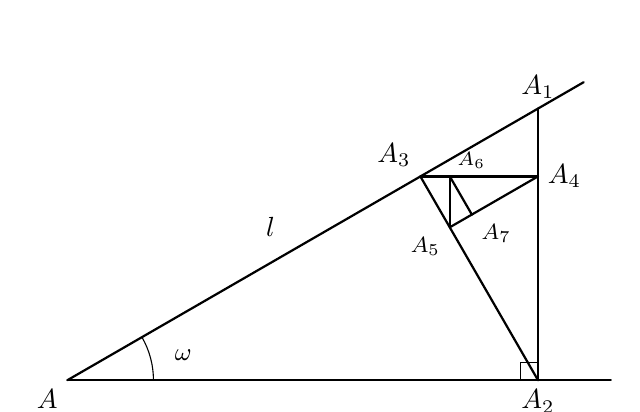
\begin{tikzpicture}[>=Stealth, scale=1.15, line cap=round, line join=round]
  % 兩直線交角 omega = 30 deg (exact perpendiculars matching original p.147)
  \coordinate (A) at (0, 0);
  \coordinate (X) at (6.0, 0);
  \coordinate (Y) at (5.7, 3.29);

  \draw[thick] (A) -- (X);
  \draw[thick] (A) -- (Y);
  \node[below left] at (A) {$A$};
  \draw[thin] (0.95, 0) arc (0:30:0.95);
  \node[font=\small] at (1.28, 0.28) {$\omega$};

  % 精確垂直足座標 (AA1 = 6, omega = 30 deg)
  \coordinate (A1) at (5.196, 3.000);
  \coordinate (A2) at (5.196, 0.000);
  \coordinate (A3) at (3.897, 2.250);
  \coordinate (A4) at (5.196, 2.250);
  \coordinate (A5) at (4.222, 1.688);
  \coordinate (A6) at (4.222, 2.250);
  \coordinate (A7) at (4.466, 1.828);

  \draw[thick] (A1) -- (A2);
  \draw[thick] (A2) -- (A3);
  \draw[thick] (A3) -- (A4);
  \draw[thick] (A4) -- (A5);
  \draw[thick] (A5) -- (A6);
  \draw[thick] (A6) -- (A7);

  \node[above] at (A1) {$A_1$};
  \node[below] at (A2) {$A_2$};
  \node[above left] at (A3) {$A_3$};
  \node[right] at (A4) {$A_4$};
  \node[below left, font=\footnotesize] at (A5) {$A_5$};
  \node[above right=-1pt, font=\scriptsize] at (A6) {$A_6$};
  \node[below right, font=\footnotesize] at (A7) {$A_7$};
  \node[above left] at (2.4, 1.48) {$l$};

  % 直角記號
  \draw[thin] (5.00, 0) -- (5.00, 0.20) -- (5.196, 0.20);
\end{tikzpicture}
\caption{無限交替垂線之幾何結構}
\label{fig:b6s-4-prob5}
\end{figure}

\paragraph{【解答】}
\begin{align*}
A_1 A_2 &= l \sin\omega \\
A_2 A_3 &= AA_2 \sin\omega = l \cos\omega \sin\omega \\
A_3 A_4 &= A_2 A_3 \sin\omega = l \cos\omega \sin^2\omega \\
A_4 A_5 &= A_3 A_4 \cos\omega = l \cos^2\omega \sin^2\omega \\
A_5 A_6 &= l \cos^2\omega \sin^3\omega \\
&\ \ \vdots
\end{align*}
即
\begin{align*}
S_1 &= l \sin\omega [1 + \cos\omega\sin\omega + (\cos\omega\sin\omega)^2 + (\cos\omega\sin\omega)^3 + \dots] \\
S_2 &= l \cos\omega\sin\omega [1 + \cos\omega\sin\omega + (\cos\omega\sin\omega)^2 + \dots]
\end{align*}
又因 $\omega$ 為銳角，$|\cos\omega\sin\omega| < 1$，故等比級數收斂，得：
\[ S_1 = \dfrac{l\sin\omega}{1-\cos\omega\sin\omega}, \quad S_2 = \dfrac{l\cos\omega\sin\omega}{1-\cos\omega\sin\omega} \]
即
\[ S = \dfrac{l\sin\omega(1+\cos\omega)}{1-\cos\omega\sin\omega} \text{。}\hfill\# \]

\paragraph{6. （39年度，臺大）}
設 $A+B+C=180^\circ$，試求下列行列式之值：
\[ \begin{vmatrix}
\sin^2 A & \cot A & 1 \\
\sin^2 B & \cot B & 1 \\
\sin^2 C & \cot C & 1
\end{vmatrix} \]

\paragraph{【分析】}
利用第二列減去第一列，第三列減去第一列，再利用三角形倍角與和角公式簡化。

\paragraph{【解答】}
\begin{align*}
\begin{vmatrix}
\sin^2 A & \cot A & 1 \\
\sin^2 B & \cot B & 1 \\
\sin^2 C & \cot C & 1
\end{vmatrix}
&= \begin{vmatrix}
\sin^2 A & \cot A & 1 \\
\sin^2 B - \sin^2 A & \cot B - \cot A & 0 \\
\sin^2 C - \sin^2 A & \cot C - \cot A & 0
\end{vmatrix} \\
&= \begin{vmatrix}
\frac{1}{2}(\cos 2A - \cos 2B) & \frac{\cos B}{\sin B} - \frac{\cos A}{\sin A} \\
\frac{1}{2}(\cos 2A - \cos 2C) & \frac{\cos C}{\sin C} - \frac{\cos A}{\sin A}
\end{vmatrix} \\
&= \begin{vmatrix}
\sin(B+A)\sin(B-A) & \frac{\sin(A-B)}{\sin A \sin B} \\
\sin(C+A)\sin(C-A) & \frac{\sin(A-C)}{\sin A \sin C}
\end{vmatrix} \\
&= \dfrac{\sin(A-B)\sin(A-C)}{\sin A \sin B \sin C} \begin{vmatrix}
-\sin(A+B) & \sin C \\
-\sin(A+C) & \sin B
\end{vmatrix} = 0
\end{align*}
因為 $\begin{cases} \sin(A+B) = \sin C \\ \sin(A+C) = \sin B \end{cases} \quad (A+B+C=180^\circ)$。\hfill$\#$

\paragraph{7.}
某學生每試五題平均可答出三題，今應試八題問至少能答出五題的或然率若干？

\paragraph{【分析】}
應先求出能答出八題、七題、六題、五題之或然率，再相加。（以上均為獨立事件）

\paragraph{【解答】}
此生答出一題之或然率為 $\dfrac{3}{5}$，不能答出一題之或然率為 $\dfrac{2}{5}$。
故能答出八題之或然率為 $\left(\dfrac{3}{5}\right)^8$，七題的為 ${}_8 C_7 \left(\dfrac{3}{5}\right)^7 \left(\dfrac{2}{5}\right)$，六題的為 ${}_8 C_6 \left(\dfrac{3}{5}\right)^6 \left(\dfrac{2}{5}\right)^2$，五題的為 ${}_8 C_5 \left(\dfrac{3}{5}\right)^5 \left(\dfrac{2}{5}\right)^3$。故得至少可答出五題的或然率為
\begin{align*}
&\left(\dfrac{3}{5}\right)^8 + {}_8 C_7 \left(\dfrac{3}{5}\right)^7 \left(\dfrac{2}{5}\right) + {}_8 C_6 \left(\dfrac{3}{5}\right)^6 \left(\dfrac{2}{5}\right)^2 + {}_8 C_5 \left(\dfrac{3}{5}\right)^5 \left(\dfrac{2}{5}\right)^3 \\
&= \dfrac{3^5}{5^8}(27 + 144 + 336 + 448) = \dfrac{46413}{78125} \text{。}\hfill\#
\end{align*}

\paragraph{8. （46年度，聯招）}
試解
\[ \begin{vmatrix}
1+x & 2 & 3 & 4 \\
1 & 2+x & 3 & 4 \\
1 & 2 & 3+x & 4 \\
1 & 2 & 3 & 4+x
\end{vmatrix} = 0 \]

\paragraph{【分析】}
顯然可看出各列的常數項均相同。

\paragraph{【解答】}
將第二、三、四行加前第一行，得
\begin{align*}
\begin{vmatrix}
1+x & 2 & 3 & 4 \\
1 & 2+x & 3 & 4 \\
1 & 2 & 3+x & 4 \\
1 & 2 & 3 & 4+x
\end{vmatrix}
&= \begin{vmatrix}
x+10 & 2 & 3 & 4 \\
x+10 & 2+x & 3 & 4 \\
x+10 & 2 & 3+x & 4 \\
x+10 & 2 & 3 & 4+x
\end{vmatrix} \\
&= (x+10) \begin{vmatrix}
1 & 2 & 3 & 4 \\
1 & 2+x & 3 & 4 \\
1 & 2 & 3+x & 4 \\
1 & 2 & 3 & 4+x
\end{vmatrix} \\
&= (x+10) \begin{vmatrix}
1 & 0 & 0 & 0 \\
1 & x & 0 & 0 \\
1 & 0 & x & 0 \\
1 & 0 & 0 & x
\end{vmatrix} = (x+10)x^3
\end{align*}
即 $(x+10)x^3 = 0$，得 $x = -10 \text{ 或 } 0$。\hfill$\#$

\paragraph{9. （50年度，聯招）}
\begin{enumerate}[label=(\alph*), leftmargin=2em]
  \item 利用絕對值之定義，方程式 $x+y=2$ 的圖形，及關於座標之對稱性，試作 $|x|+|y|=2$ 之圖。
  \item 應用 (a) 之結果試作 $|x-1|+|y-1|=2$ 之圖。
  \item 再應用 (b)，試作 $||x|-1| + ||y|-1| = 2$ 之圖。
\end{enumerate}

\paragraph{【分析】}
一個方程式 $f(x,y)=C$，若有 $f(x,y)=f(-x,y)$，表其圖形與 $y$ 軸對稱。若 $f(x,y)=f(x,-y)$，表其圖形與 $x$ 軸對稱。若 $f(x,y)=f(-x,-y)$ 表其圖形與原點對稱。若 $f(x,y)=f(y,x)$ 表其圖形與直線 $x=y$ 對稱。

\paragraph{【解答】}
\begin{enumerate}[label=(\alph*), leftmargin=2em]
  \item 因為 $|x|+|y| = |-x|+|y| = |x|+|-y| = |-x|+|-y|$。方程式 $|x|+|y|=2$ 之圖形應分別對稱於 $x$ 軸，$y$ 軸和原點，又知 $-2\le x\le 2, -2\le y\le 2$ 為必要條件。今在此範圍（第一象限）內 $x+y=2$ 的圖形如圖 1。故根據其對稱性繪出 $|x|+|y|=2$ 的圖形如圖 2（第 2, 3, 4 象限均含）。（注意：$CD$ 段亦可在畫出 $BC$ 段後根據對 $x$ 軸的對稱性而畫出）。
  \item 將座標平移到 $(1,1)$ 點，則可由 (a) 得到 $|x-1|+|y-1|=2$ 的圖形，見圖 3。
  \item 在 $x\ge 0, y\ge 0$，$||x|-1|+||y|-1|=2$ 之圖形恰當 (b) 之圖形相同。又可驗證此方程式對於 $x$ 軸、$y$ 軸、原點均對稱故可利用對稱性作圖 如圖 4。\hfill$\#$
\end{enumerate}

\begin{figure}[H]
\centering
\begin{subfigure}[b]{0.46\textwidth}
\centering
\begin{tikzpicture}[>=Stealth, scale=0.72, line cap=round]
  \draw[->] (-0.8, 0) -- (3.2, 0) node[right] {\footnotesize $X$};
  \draw[->] (0, -0.8) -- (0, 3.2) node[above] {\footnotesize $Y$};
  \draw[thick] (2, 0) -- (0, 2);
  \node[above right] at (2, 0) {\footnotesize $A$};
  \node[below] at (2, 0) {\footnotesize $2$};
  \node[above right] at (0, 2) {\footnotesize $B$};
  \node[left] at (0, 2) {\footnotesize $2$};
\end{tikzpicture}
\caption{圖 1}
\end{subfigure}
\hfill
\begin{subfigure}[b]{0.46\textwidth}
\centering
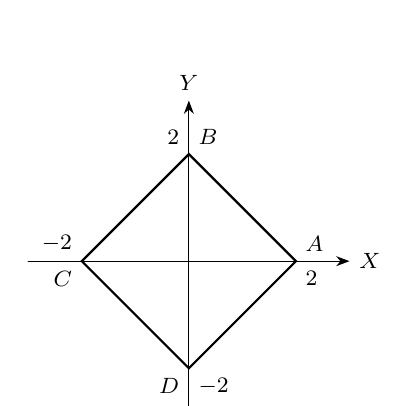
\begin{tikzpicture}[>=Stealth, scale=0.68, line cap=round]
  \draw[->] (-3.0, 0) -- (3.0, 0) node[right] {\footnotesize $X$};
  \draw[->] (0, -2.9) -- (0, 3.0) node[above] {\footnotesize $Y$};
  \draw[thick] (2, 0) -- (0, 2) -- (-2, 0) -- (0, -2) -- cycle;
  \node[above right] at (0, 2) {\footnotesize $B$};
  \node[above left] at (0, 2) {\footnotesize $2$};
  \node[above right] at (2, 0) {\footnotesize $A$};
  \node[below right] at (2, 0) {\footnotesize $2$};
  \node[above left] at (-2, 0) {\footnotesize $-2$};
  \node[below left] at (-2, 0) {\footnotesize $C$};
  \node[below left] at (0, -2) {\footnotesize $D$};
  \node[below right] at (0, -2) {\footnotesize $-2$};
\end{tikzpicture}
\caption{圖 2}
\end{subfigure}

\vspace{0.8em}
\begin{subfigure}[b]{0.46\textwidth}
\centering
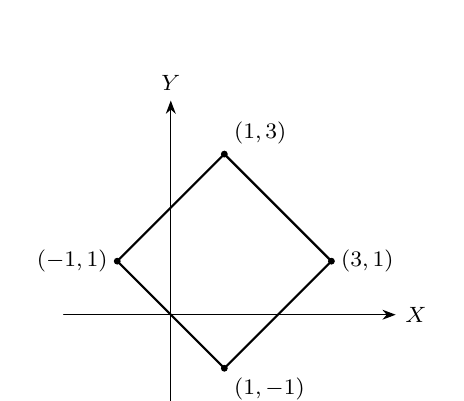
\begin{tikzpicture}[>=Stealth, scale=0.68, line cap=round]
  \draw[->] (-2.0, 0) -- (4.2, 0) node[right] {\footnotesize $X$};
  \draw[->] (0, -1.8) -- (0, 4.0) node[above] {\footnotesize $Y$};
  \draw[thick] (3, 1) -- (1, 3) -- (-1, 1) -- (1, -1) -- cycle;
  \filldraw (1, 3) circle (1.5pt) node[above right] {\footnotesize $(1,3)$};
  \filldraw (3, 1) circle (1.5pt) node[right] {\footnotesize $(3,1)$};
  \filldraw (-1, 1) circle (1.5pt) node[left] {\footnotesize $(-1,1)$};
  \filldraw (1, -1) circle (1.5pt) node[below right] {\footnotesize $(1,-1)$};
\end{tikzpicture}
\caption{圖 3}
\end{subfigure}
\hfill
\begin{subfigure}[b]{0.46\textwidth}
\centering
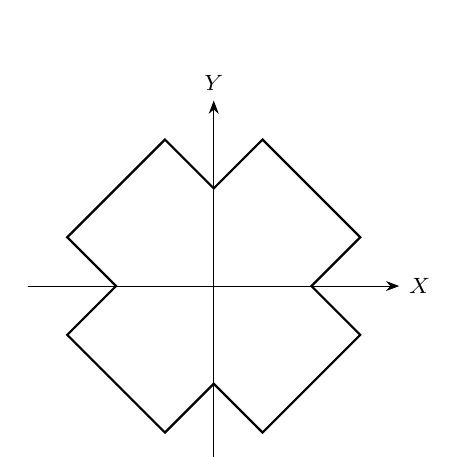
\begin{tikzpicture}[>=Stealth, scale=0.62, line cap=round]
  \draw[->] (-3.8, 0) -- (3.8, 0) node[right] {\footnotesize $X$};
  \draw[->] (0, -3.7) -- (0, 3.8) node[above] {\footnotesize $Y$};
  % 四個象限對稱拼接圖形
  \draw[thick] (3, 1) -- (1, 3) -- (0, 2) -- (-1, 3) -- (-3, 1) -- (-2, 0) -- (-3, -1) -- (-1, -3) -- (0, -2) -- (1, -3) -- (3, -1) -- (2, 0) -- cycle;
\end{tikzpicture}
\caption{圖 4}
\end{subfigure}
\caption{含絕對值之線性幾何對稱圖形}
\label{fig:b6s-4-prob9}
\end{figure}

\paragraph{10. （51年度，聯招）}
解下列不等式
\[ \begin{vmatrix}
1-x & 4 & 1 & 1 \\
1 & 2-x & 3 & 1 \\
1 & 1 & 3-x & 2 \\
1 & 1 & 1 & 4-x
\end{vmatrix} > 0 \]

\paragraph{【分析】}
同第八題，各列係數和相等，各行加到第一行。

\paragraph{【解答】}
\begin{align*}
\begin{vmatrix}
1-x & 4 & 1 & 1 \\
1 & 2-x & 3 & 1 \\
1 & 1 & 3-x & 2 \\
1 & 1 & 1 & 4-x
\end{vmatrix}
&= \begin{vmatrix}
7-x & 4 & 1 & 1 \\
7-x & 2-x & 3 & 1 \\
7-x & 1 & 3-x & 2 \\
7-x & 1 & 1 & 4-x
\end{vmatrix} \\
&= (7-x) \begin{vmatrix}
1 & 4 & 1 & 1 \\
1 & 2-x & 3 & 1 \\
1 & 1 & 3-x & 2 \\
1 & 1 & 1 & 4-x
\end{vmatrix} \\
&= (7-x) \begin{vmatrix}
1 & 4 & 1 & 1 \\
0 & -2-x & 2 & 0 \\
0 & -3 & 2-x & 1 \\
0 & -3 & 0 & 3-x
\end{vmatrix} \\
&= (7-x) \begin{vmatrix}
-2-x & 2 & 0 \\
-3 & 2-x & 1 \\
-3 & 0 & 3-x
\end{vmatrix} \\
&= (7-x) \begin{vmatrix}
-x & 2 & 0 \\
-x & 2-x & 1 \\
-x & 0 & 3-x
\end{vmatrix} \\
&= x(x-7) \begin{vmatrix}
1 & 2 & 0 \\
1 & 2-x & 1 \\
1 & 0 & 3-x
\end{vmatrix} = x(x-7) \begin{vmatrix}
1 & 2 & 0 \\
0 & -x & 1 \\
0 & -2 & 3-x
\end{vmatrix} \\
&= x(x-7) \begin{vmatrix}
-x & 1 \\
-2 & 3-x
\end{vmatrix} = x(x-7)(x-2)(x-1)
\end{align*}
故得 $x(x-1)(x-2)(x-7) > 0$。

今由下表：
\begin{center}
\renewcommand{\arraystretch}{1.2}
\begin{tabular}{c|c|c|c|c|c}
& $x<0$ & $0<x<1$ & $1<x<2$ & $2<x<7$ & $7<x$ \\ \hline
$x$ & $-$ & $+$ & $+$ & $+$ & $+$ \\
$x-1$ & $-$ & $-$ & $+$ & $+$ & $+$ \\
$x-2$ & $-$ & $-$ & $-$ & $+$ & $+$ \\
$x-7$ & $-$ & $-$ & $-$ & $-$ & $+$ \\ \hline
$f(x)$ & $+$ & $-$ & $+$ & $-$ & $+$
\end{tabular}
\end{center}
故得 $x<0$ 或 $1<x<2$ 或 $7<x$。\hfill$\#$

\paragraph{註：} 另有一簡便之法如下，從 7 的右邊起畫正、負號相間：
\begin{center}
\begin{tikzpicture}[scale=1.0]
  \draw[thick, ->] (-1, 0) -- (8.5, 0);
  \foreach \x in {0, 1, 2, 7} {
    \draw (\x, 0.1) -- (\x, -0.1) node[below] {$\x$};
  }
  \node[above] at (-0.5, 0.1) {$+$};
  \node[above] at (0.5, 0.1) {$-$};
  \node[above] at (1.5, 0.1) {$+$};
  \node[above] at (4.5, 0.1) {$-$};
  \node[above] at (7.8, 0.1) {$+$};
\end{tikzpicture}
\end{center}
故取 $7<x$ 或 $1<x<2$ 或 $x<0$。

\paragraph{11. （52年度，聯招）}
設正三角形 $ABC$ 之一邊長為 $k$；今依 $AB, BC, CA$ 之順序將其各區分為 $1:2$ 之點命為 $A_1, B_1, C_1$；其次依 $A_1 B_1, B_1 C_1, C_1 A_1$ 之順序，將三角形 $A_1 B_1 C_1$ 之各邊分為 $1:2$ 之邊命為 $A_2, B_2, C_2$；再次同樣，如此繼續無窮次，試求 $ABC, A_1 B_1 C_1, A_2 B_2 C_2, \dots$ 等無限個三角形面積之總和。

\paragraph{【分析】}
我們猜測各三角形均相似，且其面積比成一等比級數。

\paragraph{【解答】}
首先，$\angle A_1 B B_1 = \dfrac{\pi}{3}, \quad \overline{A_1 B} = 2\overline{BB_1}$，故 $\angle A_1 B_1 B = \dfrac{\pi}{2}$。所以
\[ A_1 B_1 = A_1 B \sin\dfrac{\pi}{3} = \dfrac{2}{3}k \cdot \dfrac{\sqrt{3}}{2} = \dfrac{\sqrt{3}}{3}k \]
故得知 $\triangle A_1 B_1 C_1$ 亦為正三角形，同理 $\triangle A_n B_n C_n$ 均為正三角形，故均相似。

\begin{figure}[H]
\centering
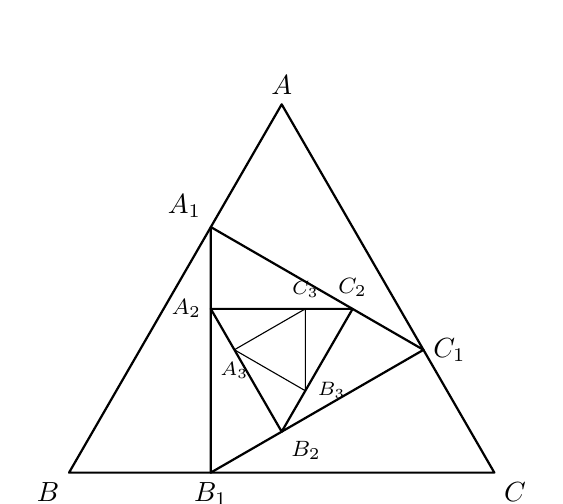
\begin{tikzpicture}[>=Stealth, scale=1.35, line cap=round, line join=round]
  \coordinate (A) at (0, 3.464);
  \coordinate (B) at (-2, 0);
  \coordinate (C) at (2, 0);

  \draw[thick] (A) -- (B) -- (C) -- cycle;
  \node[above] at (A) {$A$};
  \node[below left] at (B) {$B$};
  \node[below right] at (C) {$C$};

  % 依 AB, BC, CA 順序作 1:2 分點 (AA1:A1B = 1:2, 使 A1B1 垂直於 BC, 與原書 p.154 一致)
  \coordinate (A1) at ($(A)!0.3333!(B)$);
  \coordinate (B1) at ($(B)!0.3333!(C)$);
  \coordinate (C1) at ($(C)!0.3333!(A)$);

  \draw[thick] (A1) -- (B1) -- (C1) -- cycle;
  \node[above left] at (A1) {$A_1$};
  \node[below] at (B1) {$B_1$};
  \node[right] at (C1) {$C_1$};

  % 第二層 1:2 分點
  \coordinate (A2) at ($(A1)!0.3333!(B1)$);
  \coordinate (B2) at ($(B1)!0.3333!(C1)$);
  \coordinate (C2) at ($(C1)!0.3333!(A1)$);

  \draw[thick] (A2) -- (B2) -- (C2) -- cycle;
  \node[left, font=\footnotesize] at (A2) {$A_2$};
  \node[below right, font=\footnotesize] at (B2) {$B_2$};
  \node[above=1pt, font=\footnotesize] at (C2) {$C_2$};

  % 第三層 1:2 分點
  \coordinate (A3) at ($(A2)!0.3333!(B2)$);
  \coordinate (B3) at ($(B2)!0.3333!(C2)$);
  \coordinate (C3) at ($(C2)!0.3333!(A2)$);

  \draw[thin] (A3) -- (B3) -- (C3) -- cycle;
  \node[below=1pt, font=\scriptsize] at (A3) {$A_3$};
  \node[right=1pt, font=\scriptsize] at (B3) {$B_3$};
  \node[above=0.5pt, font=\scriptsize] at (C3) {$C_3$};
\end{tikzpicture}
\caption{無限正三角形縮小嵌套結構}
\label{fig:b6s-4-prob11}
\end{figure}

所以，
\[ \dfrac{\triangle A_1 B_1 C_1 \text{ 面積}}{\triangle ABC \text{ 面積}} = \dfrac{A_1 B_1^2}{AB^2} = \dfrac{(\frac{\sqrt{3}}{3}k)^2}{k^2} = \dfrac{1}{3} \]
即
\[ \triangle A_n B_n C_n \text{ 面積} = \dfrac{1}{3}\triangle A_{n-1} B_{n-1} C_{n-1} \text{ 面積} = \dfrac{1}{3^n}\triangle ABC \text{ 面積} \]
今 $\triangle ABC \text{ 面積} = \dfrac{\sqrt{3}}{4}k^2$
\begin{align*}
\therefore S &= \triangle ABC \text{ 面積} + \triangle A_1 B_1 C_1 \text{ 面積} + \triangle A_2 B_2 C_2 \text{ 面積} + \dots \\
&= \dfrac{\sqrt{3}}{4}k^2 \left(1 + \dfrac{1}{3} + \dfrac{1}{3^2} + \dfrac{1}{3^3} + \dots\right) = \dfrac{\sqrt{3}}{4}k^2 \cdot \dfrac{1}{1-\frac{1}{3}} = \dfrac{3\sqrt{3}}{8}k^2 \text{。}\hfill\#
\end{align*}

\paragraph{12. （53年度，聯招）}
設 $a_1, a_2, \dots, a_n; b_1, b_2, \dots, b_n$ 及 $k$ 均為實數，求下列等式中之 $p, q, r$：
\[ (ka_1+b_1)^2 + (ka_2+b_2)^2 + \dots + (ka_n+b_n)^2 = pk^2 + 2qk + r \]
並由此推出不等式
\[ (a_1 b_1 + a_2 b_2 + \dots + a_n b_n)^2 \le (a_1^2 + a_2^2 + \dots + a_n^2)(b_1^2 + b_2^2 + \dots + b_n^2) \]

\paragraph{【分析】}
顯然須利用判別式 $\ge 0$ 的性質。

\paragraph{【解答】}
由前式左邊，顯然得 $pk^2+2qk+r \ge 0$，又
\begin{align*}
p &= (a_1^2+a_2^2+\dots+a_n^2) \\
q &= (a_1 b_1 + a_2 b_2 + \dots + a_n b_n) \\
r &= (b_1^2+b_2^2+\dots+b_n^2)
\end{align*}
今 $p\ge 0$，無論 $k$ 值為何恆有 $pk^2+2qk+r \ge 0$ 的充要條件為 $q^2-pr \le 0$，即
\[ (a_1 b_1 + a_2 b_2 + \dots + a_n b_n)^2 \le (a_1^2+a_2^2+\dots+a_n^2)(b_1^2+b_2^2+\dots+b_n^2) \text{。}\hfill\# \]

\paragraph{13. （54年度，聯招）}
設 $n$ 為正整數
\begin{enumerate}[label=(\alph*), leftmargin=2em]
  \item 解方程式 $x^n-1=0$（求複數解）
  \item 證明：
  \begin{align*}
  1 + \cos\dfrac{2\pi}{n} + \cos\dfrac{4\pi}{n} + \dots + \cos\dfrac{2(n-1)\pi}{n} &= 0 \\
  \sin\dfrac{2\pi}{n} + \sin\dfrac{4\pi}{n} + \dots + \sin\dfrac{2(n-1)\pi}{n} &= 0
  \end{align*}
\end{enumerate}

\paragraph{【分析】}
\begin{enumerate}[label=(\alph*), leftmargin=2em]
  \item 顯然需用 DeMoivre 定理。
  \item 在解決 (a) 解以後，很自然想到利用根與係數關係。因在 $x^n-1=0$ 中，諸根之和為 0，又若 $a+bi=0$ 則 $a=b=0$。
\end{enumerate}

\paragraph{【解答】}
\begin{enumerate}[label=(\alph*), leftmargin=2em]
  \item $x^n = 1 = \cos 2k\pi + i\sin 2k\pi$，即
  \[ x_k = \cos\dfrac{2k\pi}{n} + i\sin\dfrac{2k\pi}{n}, \quad k=0, 1, 2, \dots, n-1 \text{ 得所求 } n \text{ 個根。} \]
  \item 因（諸根之和）$= -(x^{n-1} \text{ 的係數}) = 0$，得
  \begin{align*}
  &1 + \left(\cos\dfrac{2\pi}{n}+i\sin\dfrac{2\pi}{n}\right) + \left(\cos\dfrac{4\pi}{n}+i\sin\dfrac{4\pi}{n}\right) + \dots \\
  &\quad + \left(\cos\dfrac{2(n-1)\pi}{n}+i\sin\dfrac{2(n-1)\pi}{n}\right) = 0
  \end{align*}
  得實部與虛部分別為 0：
  \begin{align*}
  1 + \cos\dfrac{2\pi}{n} + \cos\dfrac{4\pi}{n} + \dots + \cos\dfrac{2(n-1)\pi}{n} &= 0 \\
  \sin\dfrac{2\pi}{n} + \sin\dfrac{4\pi}{n} + \dots + \sin\dfrac{2(n-1)\pi}{n} &= 0 \text{。}\hfill\#
  \end{align*}
\end{enumerate}

\paragraph{注意：} (b) 亦可由三角級數法求和。提示：令 $\alpha=\dfrac{2\pi}{n}$，則 $\sin\dfrac{\alpha}{2} = \sin\dfrac{\pi}{n}\ne 0$，考慮 $\cos\dfrac{2k\pi}{n} = \dfrac{1}{2\sin\frac{\alpha}{2}}\left(2\cos k\alpha \sin\dfrac{\alpha}{2}\right)$ 利用積化和。對 $\sin\dfrac{2k\pi}{n}$ 亦同樣做。

\paragraph{14. （54年度，聯招）}
設 $a, b$ 皆為實數，$ab\ne 0$，證明 $ax^2+2bxy-ay^2=0$ 之圖形為二直線互相垂直。

\paragraph{【分析】}
此二直線均過原點，故可分別表為 $y-m_1 x = 0$ 及 $y-m_2 x = 0$，只須驗證 $m_1 m_2 = -1$。

\paragraph{【解答】}
原式可寫為 $y^2 - 2\dfrac{b}{a}xy - x^2 = 0$。今
\[ (y-m_1 x)(y-m_2 x) = y^2 - (m_1+m_2)xy + m_1 m_2 x^2 = y^2 - 2\dfrac{b}{a}xy - x^2 \]
對應係數，得 $m_1 m_2 = -1$。\hfill$\#$

\paragraph{注意：} 亦可將 $y^2-2\dfrac{b}{a}xy-x^2$ 分解因式，解出 $m_1, m_2$，再驗證 $m_1 m_2 = -1$，但較繁複多矣。

\paragraph{15.}
已知一函數 $f(x)$ 具有下列諸性質：
\[ f(x+5) = f(x), \quad f(-x) = -f(x), \quad f\left(\dfrac{1}{3}\right) = 1 \]
試求
\begin{enumerate}[label=(\alph*), leftmargin=2em]
  \item $f\left(\dfrac{16}{3}\right)$
  \item $f\left(\dfrac{29}{3}\right)$
  \item $f(12)+f(-7)$
\end{enumerate}

\paragraph{【分析】}
這不一定是一個多項式（其實根本不是）。我們注意到 $\dfrac{16}{3} = 5+\dfrac{1}{3}, \dfrac{29}{3} = 10-\dfrac{1}{3}$。

\paragraph{【解答】}
\begin{enumerate}[label=(\alph*), leftmargin=2em]
  \item $f\left(\dfrac{16}{3}\right) = f\left(5+\dfrac{1}{3}\right) = f\left(\dfrac{1}{3}\right) = 1$
  \item $f\left(\dfrac{29}{3}\right) = f\left(5+\left(5-\dfrac{1}{3}\right)\right) = f\left(5-\dfrac{1}{3}\right) = f\left(-\dfrac{1}{3}\right) = -f\left(\dfrac{1}{3}\right) = -1$
  \item $f(12)+f(-7) = f(10+2)-f(7) = f(2)-f(2) = 0$。\hfill$\#$
\end{enumerate}

\paragraph{16. （55年度，聯招）}
設 $z = x+iy$，其中 $x, y$ 均為實數而 $i^2 = -1$。證明
\[ |z| \le |x|+|y| \le \sqrt{2}|z| \]

\paragraph{【分析】}
左邊不等式，從向量的觀點為顯然。右邊不等式可以直接去計算。

\paragraph{【解答】}
\begin{enumerate}[label=(\alph*), leftmargin=2em]
  \item $|z| = \sqrt{x^2+y^2}$。利用三角形兩邊和大於第三邊的關係，得 $|z| \le |x|+|y|$。
  \item $(|x|+|y|)^2 - (\sqrt{2}|z|)^2 = x^2+2|x||y|+y^2 - 2(x^2+y^2) = -(x^2-2|x||y|+y^2) = -(|x|-|y|)^2 \le 0$，即 $|x|+|y| \le \sqrt{2}|z|$。\hfill$\#$
\end{enumerate}

\begin{figure}[H]
\centering
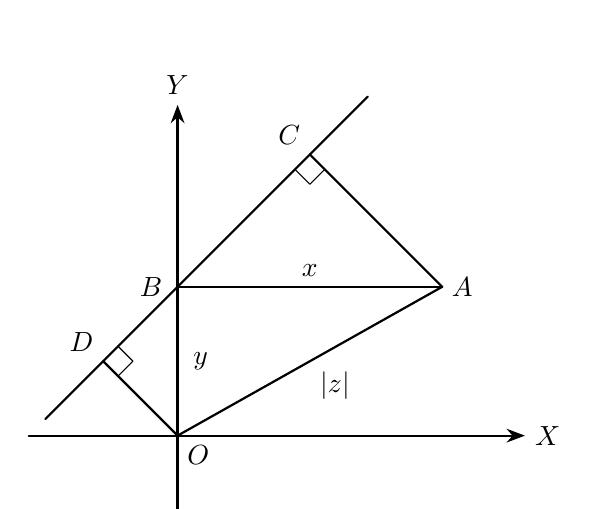
\begin{tikzpicture}[>=Stealth, scale=1.05, line cap=round, line join=round]
  \coordinate (O) at (0, 0);
  \coordinate (X) at (4.2, 0);
  \coordinate (Y) at (0, 4.0);

  \draw[->, thick] (-1.8, 0) -- (X) node[right] {$X$};
  \draw[->, thick] (0, -1.0) -- (Y) node[above] {$Y$};
  \node[below right] at (O) {$O$};

  % 點 A(x, y), B(0, y)
  \coordinate (A) at (3.2, 1.8);
  \coordinate (B) at (0, 1.8);

  \draw[thick] (O) -- (A) node[midway, below right] {$|z|$};
  \draw[thick] (B) -- (A) node[midway, above] {$x$};
  \draw[thick] (O) -- (B) node[midway, right=2pt] {$y$};
  \node[right] at (A) {$A$};
  \node[left=2pt] at (B) {$B$};

  % 過 B 斜率為 1 之直線 y = x + 1.8，以及 A, O 之正交投影 C(1.6, 3.4), D(-0.9, 0.9)
  \draw[thick] (-1.6, 0.2) -- (2.3, 4.1);
  \coordinate (C) at (1.6, 3.4);
  \coordinate (D) at (-0.9, 0.9);

  \draw[thick] (A) -- (C);
  \draw[thick] (O) -- (D);

  % 直角記號於 C 與 D
  \draw[thin] ($(C)+(-0.18,-0.18)$) -- ($(C)+(0,-0.36)$) -- ($(C)+(0.18,-0.18)$);
  \draw[thin] ($(D)+(0.18,0.18)$) -- ($(D)+(0.36,0)$) -- ($(D)+(0.18,-0.18)$);

  \node[above left] at (C) {$C$};
  \node[above left] at (D) {$D$};
\end{tikzpicture}
\caption{$|z| \le |x|+|y| \le \sqrt{2}|z|$ 之幾何投影證明}
\label{fig:b6s-4-prob16}
\end{figure}

\paragraph{注意：} (b) 亦可由幾何得到解決（考慮第一象限）：自 $B$ 作斜率為 1 的直線，則
\[ \overline{BC} = \overline{AB}\cos\dfrac{\pi}{4} = \dfrac{x}{\sqrt{2}}, \quad \overline{BD} = \overline{OB}\cos\dfrac{\pi}{4} = \dfrac{y}{\sqrt{2}} \]
今由於 $\angle ACB, \angle BDO$ 均為直角，
\[ \overline{OA} \ge \overline{CD} = \overline{BC}+\overline{BD} = \dfrac{x}{\sqrt{2}} + \dfrac{y}{\sqrt{2}} \]
即 $|z| \ge \dfrac{1}{\sqrt{2}}(|x|+|y|)$，或 $|x|+|y| \le \sqrt{2}|z|$。

\paragraph{17. （56年度，聯招）}
方程式 $\sqrt{x} - \sqrt{x+\sqrt{x-1}} = 1$ 有幾個實根？
\begin{multicols}{2}
\begin{enumerate}[label=(\Alph*)]
  \item 一個
  \item 兩個
  \item 三個
  \item 四個
  \item 以上皆非
\end{enumerate}
\end{multicols}

\paragraph{【分析】}
用最簡方式將之先有理化。

\paragraph{【解答】}
$\sqrt{x}-1 = \sqrt{x+\sqrt{x-1}}$，兩邊平方：
\[ x - 2\sqrt{x} + 1 = x + \sqrt{x-1} \implies 1-2\sqrt{x} = \sqrt{x-1} \]
再平方：
\[ 1-4\sqrt{x}+4x = x-1 \implies 2+3x = 4\sqrt{x} \]
再平方：
\[ 4+12x+9x^2 = 16x \implies 9x^2-4x+4 = 0 \]
判別式 $= 16 - 144 < 0$，無實根，故答案為 (E)。\hfill$\#$

\paragraph{注意：} 這種有開根號的方程式，就是有根也需代入原式驗證，因在平方時很可能引進一些新的或不合理的根。

\paragraph{18. （56年度，聯招）}
方程式
\[ \begin{vmatrix}
a_{11}-x & a_{12} & \dots & a_{1n} \\
a_{21} & a_{22}-x & \dots & a_{2n} \\
\vdots & \vdots & \ddots & \vdots \\
a_{n1} & a_{n2} & \dots & a_{nn}-x
\end{vmatrix} = 0 \]
諸根的乘積是：
\begin{multicols}{2}
\begin{enumerate}[label=(\Alph*)]
  \item $a_{11}+a_{22}+\dots+a_{nn}$
  \item $(-1)^n (a_{11}+a_{22}+\dots+a_{nn})$
  \item $|a_{ij}|_n$
  \item $(-1)^n |a_{ij}|_n$
  \item 以上皆非
\end{enumerate}
\end{multicols}

\paragraph{【分析】}
這是行列式與方程式論的混合題。我們知道一個多項式 $f(x)$ 的常數項為 $f(0)$。又一 $n$ 次多項式之 $n$ 次項係數除其常數項所得商之 $(-1)^n$ 為諸根之乘積。

\paragraph{【解答】}
設
\[ f(x) = \begin{vmatrix}
a_{11}-x & a_{12} & \dots & a_{1n} \\
a_{21} & a_{22}-x & \dots & a_{2n} \\
\vdots & \vdots & \ddots & \vdots \\
a_{n1} & a_{n2} & \dots & a_{nn}-x
\end{vmatrix} \]
則 $f(x)$ 為一 $n$ 次多項式，其 $n$ 次項係數為 $(-1)^n$，常數項 $f(0) = |a_{ij}|_n$。故諸根乘積 $= (-1)^n \dfrac{|a_{ij}|_n}{(-1)^n} = |a_{ij}|_n$。答案為 (C)。\hfill$\#$

\paragraph{19. （57年度，聯招）}
兩觀測站 $S_1, S_2$ 之距離為 $r$；飛機 $A$ 在地面 $B$ 點上空。$S_1$ 站測得 $A$ 之仰角為 $\phi$。$\angle BS_1 S_2 = \psi$；$S_2$ 站測得 $\angle BS_2 S_1 = \theta$，則飛機高 $\overline{AB}$ 為：
\begin{multicols}{2}
\begin{enumerate}[label=\tiangan*]
  \item $r\dfrac{\sin\theta\sin\phi}{\sin(\theta+\psi)}$
  \item $r\dfrac{\sin\theta\tan\phi}{\sin(\theta+\psi)}$
  \item $r\dfrac{\cot\phi\cot\psi+\sqrt{\cot^2\phi\csc^2\psi-\cot^2\theta}}{\cot^2\theta-\cot^2\psi}$
  \item $r\dfrac{\cot\phi\cot\psi-\sqrt{\cot^2\phi\csc^2\psi-\cot^2\theta}}{\cot^2\theta-\cot^2\psi}$
  \item 以上皆非
\end{enumerate}
\end{multicols}

\begin{figure}[H]
\centering
\begin{tikzpicture}[>=Stealth, scale=1.05, line cap=round, line join=round]
  \coordinate (S1) at (0, 0);
  \coordinate (S2) at (4.8, 0);
  \coordinate (B) at (3.2, 1.7);
  \coordinate (A) at (3.2, 4.1);

  \draw[thick] (S1) -- (S2) node[midway, below] {$r$};
  \draw[thick] (S1) -- (B);
  \draw[thick] (S2) -- (B);
  \draw[line width=1.4pt] (B) -- (A) node[midway, left=3pt] {高};
  \draw[thick] (S1) -- (A);
  \draw[dashed] (S2) -- (A);

  % 直角記號於 B (AB 垂直地面 S1B)
  \draw[thin] (3.2, 1.98) -- (2.96, 1.85) -- (2.96, 1.57);

  \node[below left] at (S1) {$S_1$};
  \node[below right] at (S2) {$S_2$};
  \node[above] at (A) {$A$};
  \node[right=2pt] at (B) {$B$};

  \draw[thin] (0.95, 0) arc (0:28:0.95);
  \node[font=\small] at (1.22, 0.25) {$\psi$};
  \draw[thin] (0.72, 0.38) arc (28:52:0.82);
  \node[font=\small] at (0.85, 0.72) {$\phi$};
  \draw[thin] (4.15, 0) arc (180:133:0.65);
  \node[font=\small] at (4.05, 0.28) {$\theta$};
\end{tikzpicture}
\caption{飛機高度之立體三角觀測模型}
\label{fig:b6s-4-prob19}
\end{figure}

\paragraph{【解答】}
$\overline{AB} = \overline{S_1 B}\tan\phi$。又在 $\triangle S_1 B S_2$ 中，由正弦定理：
\[ \dfrac{\sin\theta}{\overline{S_1 B}} = \dfrac{\sin(\pi-(\psi+\theta))}{r} \implies \overline{S_1 B} = \dfrac{r\sin\theta}{\sin(\psi+\theta)} \]
故
\[ \overline{AB} = \overline{S_1 B}\tan\phi = \dfrac{r\sin\theta\tan\phi}{\sin(\psi+\theta)} \]
故答案為 (乙)。\hfill$\#$

\paragraph{20. （57年度，聯招）}
方程式 $x^2+4xy+4y^2-2x-4y-3=0$ 的圖形是：
\begin{multicols}{2}
\begin{enumerate}[label=\tiangan*]
  \item 橢圓
  \item 雙曲線
  \item 兩平行直線之聯集
  \item 兩相交直線之聯集
  \item 以上皆非
\end{enumerate}
\end{multicols}

\paragraph{【解答】}
$B^2-AC = 4-4=0$ 為直線，因式分解：
\begin{align*}
x^2+(4y-2)x+(4y^2-4y-3) &= 0 \\
x^2+2(2y-1)x+(2y+1)(2y-3) &= 0 \\
(x+2y+1)(x+2y-3) &= 0
\end{align*}
所得二直線 $x+2y+1=0, x+2y-3=0$ 為平行。答案為 (丙)。\hfill$\#$

\paragraph{21. （57年度，聯招）}
令 $O$ 為 $\triangle ABC$ 內部之一點，設射線 $\vec{AO}$ 交 $\overline{BC}$ 於 $D$，$\vec{BO}$ 交 $\overline{CA}$ 於 $E$，$\vec{CO}$ 交 $\overline{AB}$ 於 $F$。令 $P = AB+BC+CA, q = AD+BE+CF$。則必有：
\begin{multicols}{2}
\begin{enumerate}[label=\tiangan*]
  \item $q < \frac{1}{3}P$
  \item $\frac{1}{3}P \le q \le \frac{1}{2}P$
  \item $\frac{1}{2}P < q < \frac{3}{2}P$
  \item $\frac{3}{2}P \le q \le 2P$
  \item 以上皆非
\end{enumerate}
\end{multicols}

\begin{figure}[H]
\centering
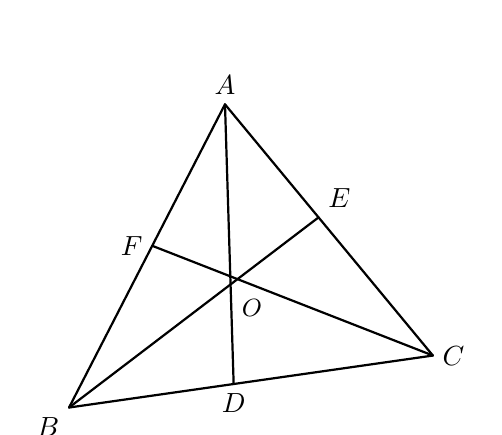
\begin{tikzpicture}[>=Stealth, scale=1.1, line cap=round, line join=round]
  \coordinate (A) at (1.8, 3.5);
  \coordinate (B) at (0, 0);
  \coordinate (C) at (4.2, 0.6);

  % 重心內部點 O 及三條準確共點塞瓦線
  \coordinate (D) at (1.9, 0.271);
  \coordinate (E) at (2.88, 2.195);
  \coordinate (F) at (0.96, 1.867);
  \coordinate (O) at (1.84, 1.40);

  \draw[thick] (A) -- (B) -- (C) -- cycle;
  \draw[thick] (A) -- (D);
  \draw[thick] (B) -- (E);
  \draw[thick] (C) -- (F);

  \node[above] at (A) {$A$};
  \node[below left] at (B) {$B$};
  \node[right] at (C) {$C$};
  \node[below] at (D) {$D$};
  \node[above right] at (E) {$E$};
  \node[left] at (F) {$F$};
  \node[below right=1pt, font=\small] at (1.86, 1.38) {$O$};
\end{tikzpicture}
\caption{三角形內部線段之不等式關係}
\label{fig:b6s-4-prob21}
\end{figure}

\paragraph{【解答】}
在 $\triangle ABD$ 中，$AB < AD+BD$；於 $\triangle ACD$ 中，$AC < AD+CD$。兩邊相加：
\[ AB+AC < 2AD+BC \implies AB+AC-BC < 2AD \]
同理 $AB+BC-AC < 2BE, AC+BC-AB < 2CF$。三式相加得：
\[ \dfrac{1}{2}(AB+BC+CA) < AD+BE+CF \tag{1} \]
又在 $\triangle ABD$ 中，$AD < AB+BD$；於 $\triangle ACD$ 中，$AD < AC+CD$。邊邊相加得 $2AD < AB+AC+BC$。同理可得
\[ AD+BE+CF < \dfrac{3}{2}(AB+BC+AC) \tag{2} \]
綜合 (1), (2) 得 $\dfrac{1}{2}P < q < \dfrac{3}{2}P$。答案：丙。\hfill$\#$

\paragraph{22. （57年度，聯招）}
方程式 $\log_6 x + \log_6(x^2-7) = 1$ 的解集合之元素個數為：
\begin{multicols}{2}
\begin{enumerate}[label=\tiangan*]
  \item 0
  \item 1
  \item 2
  \item 3
  \item 以上皆非
\end{enumerate}
\end{multicols}

\paragraph{【解答】}
由原式得 $\log_6 x(x^2-7) = 1 \implies x(x^2-7) = 6 \implies x^3-7x-6 = 0$。
分解得 $(x+1)(x+2)(x-3) = 0$。
因需 $x>0, x^2-7>0$，故只能取 $x=3$。元素個數為 1。答案：(乙)（原書誤寫為丁，實為 1 個解，即乙）。\hfill$\#$

\paragraph{23. （58年度，聯招）}
設 $a, b$ 為實數，若已知方程式 $x^3+ax+b=0$ 之一複數根為 $1+i$，則 $\dfrac{a}{b}$ 滿足下列不等式：
\begin{multicols}{2}
\begin{enumerate}[label=\tiangan*]
  \item $-1 \le \frac{a}{b} < -\frac{2}{3}$
  \item $-\frac{2}{3} \le \frac{a}{b} < -\frac{1}{3}$
  \item $-\frac{1}{3} \le \frac{a}{b} < 0$
  \item $0 \le \frac{a}{b} < \frac{1}{3}$
  \item $\frac{1}{3} \le \frac{a}{b} < \frac{2}{3}$
  \item $\frac{2}{3} \le \frac{a}{b} < 1$
  \item $1 \le \frac{a}{b} < \frac{4}{3}$
  \item $\frac{4}{3} \le \frac{a}{b} < \frac{5}{3}$
\end{enumerate}
\end{multicols}

\paragraph{【解答】}
實係數方程式有根 $1+i$，必有共軛根 $1-i$。故
\[ x^3+ax+b \text{ 能為 } (x-1-i)(x-1+i) = x^2-2x+2 \text{ 所整除。} \]
令 $x^3+ax+b = (x^2-2x+2)(x-\alpha) = x^3 - (\alpha+2)x^2 + (2+2\alpha)x - 2\alpha$。
得 $\alpha = -2, a = 2+2\alpha = -2, b = 4$。
故 $\dfrac{a}{b} = -\dfrac{1}{2}$。答案：(乙)。\hfill$\#$

\paragraph{24. （58年度，聯招）}
$xyz$ 一平面之一點 $(1, 0, -1)$ 及一直線 $\dfrac{x-1}{4} = \dfrac{y-2}{5} = \dfrac{z-3}{6}$ 決定一平面，其平面方程式為：
\begin{multicols}{2}
\begin{enumerate}[label=\tiangan*]
  \item $x-2y+z+1=0$
  \item $x-2y+z=0$
  \item $x-2y+z-1=0$
  \item $2x-y+2z+1=0$
  \item $2x-y+2z-1=0$
  \item $2x-y+2z=0$
  \item $x-2y+2z+1=0$
  \item $x-2y+2z-1=0$
\end{enumerate}
\end{multicols}

\paragraph{【解答】}
平面設為 $a(x-1)+by+c(z+1)=0$。直線上一點 $(1, 2, 3)$ 在平面上，得 $2b+4c=0$；直線方向向量 $(4,5,6)$ 與法向量垂直，得 $4a+5b+6c=0$。
解得 $b=-2c, a=c$。代入得 $c(x-1)-2c(y-0)+c(z+1)=0 \implies x-2y+z=0$。答案：(乙)。\hfill$\#$

\paragraph{25. （58年度，聯招）}
給予二正整數 $n$ 及 $M$，設 $n$ 階方陣 $[z_{jk}]$ 之元 $z_{jk} = x_{jk} + i y_{jk}$，$x_{jk}, y_{jk}$ 均為整數，其絕對值滿足 $|x_{jk}| \le M, |y_{jk}| \le M$，且 $\bar{z}_{jk} = z_{kj}$。則此類方陣共有：
\begin{multicols}{2}
\begin{enumerate}[label=\tiangan*]
  \item $(2M+1)^{\frac{n(n+1)}{2}}$
  \item $(2n+1)^{\frac{M(M+1)}{2}}$
  \item $M^n \cdot n^{\frac{n(n+1)}{2}}$
  \item $M^{\frac{n(n+1)}{2}}$
  \item $(2M+1)^{n^2} \cdot n^{\frac{n(n+1)}{2}}$
  \item $(2M+1)^{n(n+1)}$
  \item $(2M+1)^{n^2}$
  \item $n^{2(2M+1)}$
\end{enumerate}
\end{multicols}

\paragraph{【解答】}
\begin{enumerate}[label=\arabic*., leftmargin=2em]
  \item $x_{jk}$ 可取 $-M, -M+1, \dots, 0, \dots, M$，共 $2M+1$ 種；$y_{jk}$ 亦有 $2M+1$ 種。故一般元素有 $(2M+1)^2$ 種取法。
  \item 對角線上之元 $z_{ii}$ 滿足 $\bar{z}_{ii} = z_{ii}$，故 $y_{ii} = 0$，僅有實部 $x_{ii}$，共 $2M+1$ 種取法。
  \item 由於對稱性，由主對角線及下三角（或上三角）的元素決定整個方陣。
  下三角非對角元素共 $\dfrac{n(n-1)}{2}$ 個，每個有 $(2M+1)^2$ 種取法；對角線上 $n$ 個元素，每個有 $2M+1$ 種取法。
  故總共有
  \[ [(2M+1)^2]^{\frac{n(n-1)}{2}} \cdot (2M+1)^n = (2M+1)^{n(n-1)+n} = (2M+1)^{n^2} \text{ 種。} \]
  答案：(庚)。\hfill$\#$
\end{enumerate}

\paragraph{26. （58年度，聯招）}
不等式 $(|x|-1)^2 + (|y|-2)^2 \le 5$ 之解集合為 $xy$ 一平面上之一區域，此區域之面積為：
\begin{multicols}{2}
\begin{enumerate}[label=\tiangan*]
  \item $2(5\pi+8)$
  \item $3(4\pi+3)$
  \item $4(3\pi+2)$
  \item $5(2\pi+3)$
  \item $6\left(2\pi+\frac{5}{2}\right)$
  \item $8\left(\pi+\frac{5}{2}\right)$
  \item $10\left(\pi+\frac{4}{5}\right)$
  \item $12\left(\pi+\frac{4}{3}\right)$
\end{enumerate}
\end{multicols}

\begin{figure}[H]
\centering
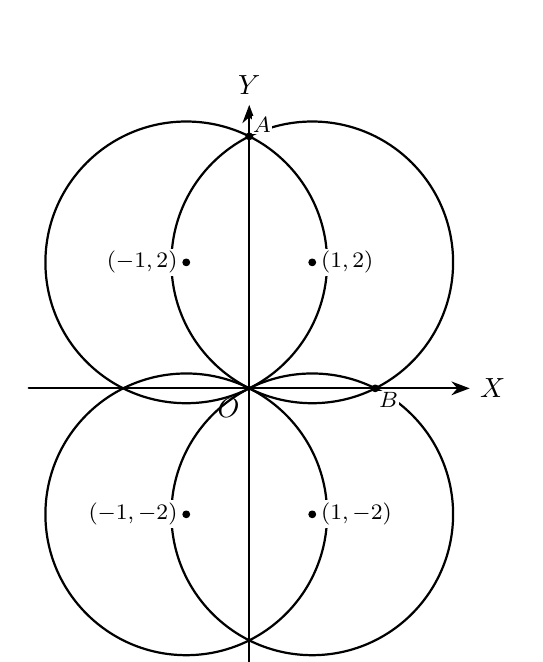
\begin{tikzpicture}[>=Stealth, scale=0.8, line cap=round, line join=round]
  \draw[->, thick] (-3.5, 0) -- (3.5, 0) node[right] {$X$};
  \draw[->, thick] (0, -4.5) -- (0, 4.5) node[above] {$Y$};
  \node[below left] at (0, 0) {$O$};

  % 四個圓心 (1,2), (-1,2), (-1,-2), (1,-2), 半徑 sqrt(5) ~= 2.236
  \draw[thick] (1, 2) circle (2.236);
  \draw[thick] (-1, 2) circle (2.236);
  \draw[thick] (-1, -2) circle (2.236);
  \draw[thick] (1, -2) circle (2.236);

  \filldraw (1, 2) circle (1.5pt) node[right=2pt, fill=white, inner sep=1pt] {\footnotesize $(1,2)$};
  \filldraw (-1, 2) circle (1.5pt) node[left=2pt, fill=white, inner sep=1pt] {\footnotesize $(-1,2)$};
  \filldraw (-1, -2) circle (1.5pt) node[left=2pt, fill=white, inner sep=1pt] {\footnotesize $(-1,-2)$};
  \filldraw (1, -2) circle (1.5pt) node[right=2pt, fill=white, inner sep=1pt] {\footnotesize $(1,-2)$};

  \coordinate (A) at (0, 4);
  \coordinate (B) at (2, 0);
  \filldraw (A) circle (1.5pt) node[above right=1pt, fill=white, inner sep=0.5pt] {\footnotesize $A$};
  \filldraw (B) circle (1.5pt) node[below right=1pt, fill=white, inner sep=0.5pt] {\footnotesize $B$};
\end{tikzpicture}
\caption{四圓相交重疊區域之對稱面積}
\label{fig:b6s-4-prob26}
\end{figure}

\paragraph{【解答】}
在四個象限各有一圓心在 $(\pm 1, \pm 2)$ 半徑為 $\sqrt{5}$ 的圓。兩圓相交之重疊區域面積經計算為 $\dfrac{5\pi}{2}-4$。
故所求總面積為 $4 \times 5\pi - 4\left(\dfrac{5\pi}{2}-4\right) = 2(5\pi+8)$。答案：(甲)。\hfill$\#$

\paragraph{27. （59年度，聯招）}
設 $z$ 為複數，則 $|z-2|+|z+2|=6$ 之解集合在複數平面之圖形為：
\begin{multicols}{2}
\begin{enumerate}[label=\tiangan*]
  \item 相交二直線
  \item 正方形
  \item 圓
  \item 橢圓
  \item 雙曲線
  \item 一直線
\end{enumerate}
\end{multicols}

\paragraph{【解答】}
令 $z=x+iy$，原式即 $\sqrt{(x-2)^2+y^2} + \sqrt{(x+2)^2+y^2} = 6$。
表示點 $(x,y)$ 到兩焦點 $(2,0), (-2,0)$ 之距離和恆為常數 $6 > 4$，故其軌跡為一橢圓。答案：(丁)。\hfill$\#$

\begin{figure}[H]
\centering
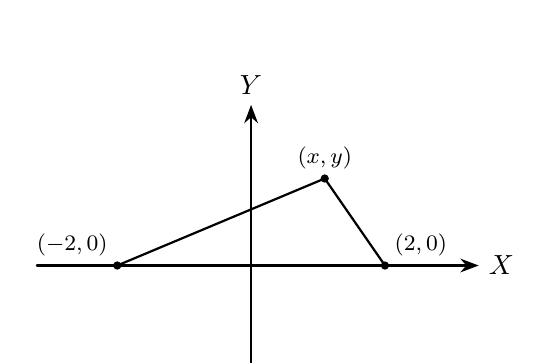
\begin{tikzpicture}[>=Stealth, scale=0.85, line cap=round, line join=round]
  \draw[->, thick] (-3.2, 0) -- (3.4, 0) node[right] {$X$};
  \draw[->, thick] (0, -1.6) -- (0, 2.4) node[above] {$Y$};
  \coordinate (F1) at (-2, 0);
  \coordinate (F2) at (2, 0);
  \coordinate (P) at (1.1, 1.3);
  \draw[thick] (F1) -- (P) -- (F2);
  \filldraw (F1) circle (1.5pt) node[above left] {\footnotesize $(-2,0)$};
  \filldraw (F2) circle (1.5pt) node[above right] {\footnotesize $(2,0)$};
  \filldraw (P) circle (1.5pt) node[above] {\footnotesize $(x,y)$};
\end{tikzpicture}
\end{figure}

\paragraph{28. （59年度，聯招）}
設 $a_n = 1+2+\dots+n$，則無窮級數 $\dfrac{1}{a_1}+\dfrac{1}{a_2}+\dots+\dfrac{1}{a_n}+\dots$ 之和等於多少？

\paragraph{【解答】}
$a_n = \dfrac{n(n+1)}{2} \implies \dfrac{1}{a_n} = \dfrac{2}{n(n+1)} = 2\left(\dfrac{1}{n} - \dfrac{1}{n+1}\right)$。
故
\[ S_n = 2\left[\left(1-\dfrac{1}{2}\right) + \left(\dfrac{1}{2}-\dfrac{1}{3}\right) + \dots + \left(\dfrac{1}{n}-\dfrac{1}{n+1}\right)\right] = 2\left(1-\dfrac{1}{n+1}\right) \longrightarrow 2 \quad (n\to\infty) \text{。}\hfill\# \]

\paragraph{29. （59年度，聯招）}
空間中有二平行線，其方程式分別為
\[ \dfrac{x}{2} = \dfrac{y-1}{1} = \dfrac{z-2}{-1} \quad \text{及} \quad \dfrac{x-1}{2} = \dfrac{y+1}{1} = \dfrac{z-8}{-1} \]
求此二直線之間的距離。

\begin{figure}[H]
\centering
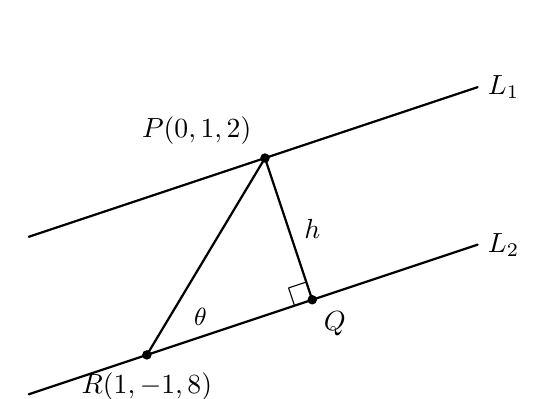
\begin{tikzpicture}[>=Stealth, scale=1.0, line cap=round, line join=round]
  % 兩平行線 L1, L2 (斜率 1/3)
  \draw[thick] (-1.0, 1.6) -- (4.7, 3.5) node[right] {$L_1$};
  \draw[thick] (-1.0, -0.4) -- (4.7, 1.5) node[right] {$L_2$};

  \coordinate (P) at (2.0, 2.6);
  \coordinate (Q) at (2.6, 0.8);
  \coordinate (R) at (0.5, 0.1);

  \draw[thick] (P) -- (Q) node[midway, right=2pt] {$h$};
  \draw[thick] (P) -- (R);

  % 直角記號於 Q (PQ 垂直 L2)
  \draw[thin] ($(Q)+(-0.075,0.225)$) -- ($(Q)+(-0.30,0.15)$) -- ($(Q)+(-0.225,-0.075)$);

  \filldraw (P) circle (1.5pt) node[above left=2pt] {$P(0,1,2)$};
  \filldraw (R) circle (1.5pt) node[below=3pt] {$R(1,-1,8)$};
  \filldraw (Q) circle (1.5pt) node[below right=1pt] {$Q$};
  \node[font=\small] at (1.18, 0.58) {$\theta$};
\end{tikzpicture}
\caption{空間兩平行直線距離幾何投影}
\label{fig:b6s-4-prob29}
\end{figure}

\paragraph{【解答】}
取 $L_1$ 上一點 $P(0,1,2)$，$L_2$ 上一點 $R(1,-1,8)$。方向向量 $\vec{u} = (2,1,-1)$，$\vec{RP} = (-1, 2, -6)$。
\begin{align*}
\cos\theta &= \dfrac{\vec{u}\cdot\vec{RP}}{|\vec{u}||\vec{RP}|} = \dfrac{-2+2+6}{\sqrt{6}\sqrt{41}} = \dfrac{6}{\sqrt{246}}, \\
h &= |\vec{RP}|\sin\theta = \sqrt{41}\sqrt{1-\dfrac{36}{246}} = \sqrt{41}\sqrt{\dfrac{210}{246}} = \sqrt{35} \text{。}\hfill\#
\end{align*}

\paragraph{30. （60年度，聯招）}
以 $x+1$ 除 $6x^3-x^2+2$，所得餘數為：
\begin{multicols}{2}
\begin{enumerate}[label=\tiangan*]
  \item $-5$
  \item $-1$
  \item 2
  \item 3
  \item 7
  \item 9
\end{enumerate}
\end{multicols}

\paragraph{【解答】}
由餘式定理，餘數 $= f(-1) = 6(-1)^3 - (-1)^2 + 2 = -6-1+2 = -5$。答案：(甲)。\hfill$\#$

\paragraph{31. （60年度，聯招）}
設 $\alpha, \beta$ 為二角，並令
\[ \begin{pmatrix} \cos\alpha & -\sin\alpha \\ \sin\alpha & \cos\alpha \end{pmatrix} \begin{pmatrix} \cos\beta & \sin\beta \\ -\sin\beta & \cos\beta \end{pmatrix} = \begin{pmatrix} a & b \\ -a & a \end{pmatrix} \]
則 $b$ 為：
\begin{multicols}{2}
\begin{enumerate}[label=\tiangan*]
  \item $\sin(\alpha+\beta)$
  \item $\cos(\alpha+\beta)$
  \item $\sin(\alpha-\beta)$
  \item $\cos(\alpha-\beta)$
  \item $\sin(\beta-\alpha)$
  \item $-\cos(\beta-\alpha)$
\end{enumerate}
\end{multicols}

\paragraph{【解答】}
由矩陣乘法，第一列第二行元素為：
\[ b = \cos\alpha\sin\beta - \sin\alpha\cos\beta = \sin(\beta-\alpha) \]
答案：(戊)。\hfill$\#$

\paragraph{31*. （60年度，聯招）}\phantomsection\label{note:b6s-ch4-p172-prob-dup}\footnote{【原書註記】：原書此處連續兩題編號皆為 31，本題實為接續之第 32 題，為保持與原書查閱對照之精確性，特加星號註記。}
平面 $x+y+z=4$ 截球面 $(x-1)^2+(y-1)^2+(z-1)^2=1$ 於一圓，此圓之面積為多少？

\begin{figure}[H]
\centering
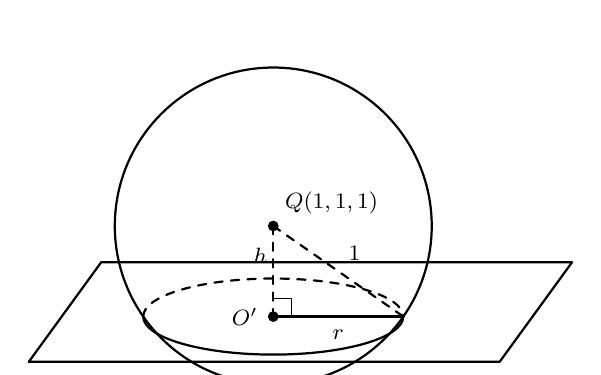
\begin{tikzpicture}[>=Stealth, scale=1.15, line cap=round, line join=round]
  % 球面與平面截圓 (與原書 p.173 一致，放大半徑避免標籤穿線)
  \coordinate (O) at (0, 1.35);
  \draw[thick] (O) circle (1.75);
  \filldraw (O) circle (1.5pt) node[above right=1pt, font=\footnotesize] {$Q(1,1,1)$};

  % 截面橢圓 (y=0.35, 半長軸 sqrt(1.75^2 - 1^2) = 1.436)
  \coordinate (Oprime) at (0, 0.35);
  \coordinate (A) at (1.436, 0.35);
  \draw[thick] (-1.436, 0.35) arc (180:360:1.436 and 0.42);
  \draw[thick, dashed] (-1.436, 0.35) arc (180:0:1.436 and 0.42);
  \filldraw (Oprime) circle (1.5pt) node[left=2pt, font=\footnotesize] {$O'$};

  \draw[thick, dashed] (O) -- (Oprime);
  \node[left=1.5pt, fill=white, inner sep=0.5pt, font=\footnotesize] at (0, 1.02) {$h$};
  \draw[thick, dashed] (O) -- (A) node[midway, above right, font=\footnotesize] {$1$};
  \draw[thick] (Oprime) -- (A) node[midway, below=1pt, font=\footnotesize] {$r$};
  % 直角記號
  \draw[thin] (0, 0.55) -- (0.20, 0.55) -- (0.20, 0.35);

  % 平面示意
  \draw[thick] (-2.7, -0.15) -- (2.5, -0.15) -- (3.3, 0.95) -- (-1.9, 0.95) -- cycle;
\end{tikzpicture}
\caption{平面截球面所成圓面積之立體幾何模型}
\label{fig:b6s-4-prob31bis}
\end{figure}

\paragraph{【解答】}
\begin{enumerate}[label=(\arabic*), leftmargin=2em]
  \item 球心 $Q(1,1,1)$ 至平面 $x+y+z-4=0$ 的距離：
  \[ h = \dfrac{|1+1+1-4|}{\sqrt{1+1+1}} = \dfrac{1}{\sqrt{3}} \]
  \item 圓的半徑 $r = \sqrt{1^2-h^2} = \sqrt{1-\dfrac{1}{3}} = \sqrt{\dfrac{2}{3}}$。
  \item 圓之面積為 $\pi r^2 = \dfrac{2}{3}\pi$。\hfill$\#$
\end{enumerate}

\paragraph{32. （61年度，聯招）}
聯立不等式
\[ \begin{cases} 0 < x < 2\pi \\ \sin x \cos^3 x > \sin^3 x \cos x \end{cases} \]
之解集合為：

\paragraph{【解答】}
$\sin x \cos x(\cos^2 x - \sin^2 x) > 0 \implies \dfrac{1}{2}\sin 2x \cos 2x > 0 \implies \dfrac{1}{4}\sin 4x > 0$。
故 $2n\pi < 4x < (2n+1)\pi \implies \dfrac{n\pi}{2} < x < (2n+1)\dfrac{\pi}{4}$。
在 $0<x<2\pi$ 內，解集合為：
\[ 0 < x < \dfrac{\pi}{4}, \quad \dfrac{\pi}{2} < x < \dfrac{3\pi}{4}, \quad \pi < x < \dfrac{5\pi}{4}, \quad \dfrac{3\pi}{2} < x < \dfrac{7\pi}{4} \text{。}\hfill\# \]

\paragraph{33. （61年度，聯招）}
下表係錄自60年度綜合所得稅申報表中之一段：

\begin{center}
\textbf{第一表\quad 綜合所得稅稅率表}

\small
\renewcommand{\arraystretch}{1.2}
\begin{tabular}{|c|l|c|}
\hline
級別 & 級\qquad 距 & 稅率 \\ \hline
1 & 綜合所得淨額在 3 萬元以下的 & $6\%$ \\
2 & 綜合所得淨額超過 3 萬元到 6 萬元之間的 & $8\%$ \\
3 & 綜合所得淨額超過 6 萬元到 10 萬元之間的 & $10\%$ \\
4 & 綜合所得淨額超過 10 萬元到 15 萬元之間的 & $12\%$ \\ \hline
\end{tabular}

\vspace{0.8em}
\textbf{第二表\quad 速算公式表}

\begin{tabular}{|c|r@{\ }c@{\ }l|}
\hline
級別 & \multicolumn{3}{c|}{綜合所得淨額 $\times$ 稅率 $-$ 累進差額 $=$ 全年應納稅額} \\ \hline
1 & 綜合所得淨額 $\times 0.06$ & $-$ & $0$ 元 $=$ 全年應納稅額 \\
2 & 綜合所得淨額 $\times 0.08$ & $-$ & $600$ 元 $=$ 全年應納稅額 \\
3 & 綜合所得淨額 $\times 0.10$ & $-$ & $1800$ 元 $=$ 全年應納稅額 \\
4 & 綜合所得淨額 $\times 0.12$ & $-$ & $3800$ 元 $=$ 全年應納稅額 \\ \hline
\end{tabular}
\end{center}

今設綜合所得淨額為 $x$，全年應納所得稅額為 $y$，則 $y$ 為 $x$ 的函數。
\begin{enumerate}[label=\arabic*), leftmargin=2em]
  \item 根據第一表將各級之 $x, y$ 的關係式分別列出。
  \item 由此結果導出第二表的速算公式。
  \item 將第一級到第 4 級 $x, y$ 間的關係用單一個式子表示出來。
\end{enumerate}

\paragraph{【解答】}
\begin{enumerate}[label=\arabic*), leftmargin=2em]
  \item 
  \begin{align*}
  \text{在 } 0\le x\le 30000: &\quad y = x \times 0.06 \tag{1} \\
  \text{在 } 30000 < x \le 60000: &\quad y = (x-30000)\times 0.08 + 30000\times 0.06 \tag{2} \\
  \text{在 } 60000 < x \le 100000: &\quad y = (x-60000)\times 0.10 + 30000\times 0.08 + 30000\times 0.06 \tag{3} \\
  \text{在 } 100000 < x \le 150000: &\quad y = (x-100000)\times 0.12 + 40000\times 0.10 \\
  &\quad\quad + 30000\times 0.08 + 30000\times 0.06 \tag{4}
  \end{align*}
  \item 
  從 (1): $y = x\times 0.06 - 0$ 為第一級\\
  從 (2): $y = x\times 0.08 - 600$ 為第二級\\
  從 (3): $y = x\times 0.10 - 1800$ 為第三級\\
  從 (4): $y = x\times 0.12 - 3800$ 為第四級
  \item 令函數為
  \[ y = ax + b|x-30000| + c|x-60000| + d|x-100000| + e \]
  經分段比較係數，解得
  \[ a=0.09, \quad b=0.01, \quad c=0.01, \quad d=0.01, \quad e=-1900 \]
  故原方程式為
  \[ y = 0.09x + 0.01|x-30000| + 0.01|x-60000| + 0.01|x-100000| - 1900 \text{。}\hfill\# \]
\end{enumerate}

\begin{center}
\textbf{63 年聯考（甲丙組）}
\end{center}

\paragraph{1. （63年度，聯招）}
設 $m, n$ 為任意正整數，且 $m>n$。令 $x=m^2-n^2, y=2mn, z=m^2+n^2$。譬如說 $m=2, n=1$，則 $x=3, y=4, z=5$，而下列各敘述成立。今問其中那些敘述在一般情形恆成立？
\begin{multicols}{2}
\begin{enumerate}[label=(\Alph*)]
  \item $x < y$
  \item $x+y > z$
  \item $x, y$ 中必有一數為 4 之倍數
  \item $x, y$ 中必有一數為 3 之倍數
  \item $x, y, z$ 中必有一數為 5 之倍數
\end{enumerate}
\end{multicols}

\paragraph{【解答】}
(B), (C), (D), (E) 為真。（第一冊，第三章）。\hfill$\#$

\paragraph{2. （63年度，聯招）}
三直線 $x-y-9=0, x+2y=0$ 及 $3x-y-7=0$ 圍成一三角形，設此三角形外接圓的方程式為 $x^2+y^2+ax+by+c=0$，則
\begin{multicols}{2}
\begin{enumerate}[label=(\Alph*)]
  \item 此三角形的三個頂點都在第四象限
  \item $a+b=8$
  \item $2a-b=20$
  \item 外接圓圓心的坐標為 $(2, -6)$
  \item $a^2+b^2-4c=100$
\end{enumerate}
\end{multicols}

\paragraph{【解答】}
解出三直線的交點為 $(6,-3), (-1,-10), (2,-1)$。代入圓方程式得：
\[ a = -4, \quad b = 12, \quad c = 15 \]
圓心為 $(2, -6)$，$a+b = 8$，$a^2+b^2-4c = 16+144-60 = 100$。
答案：(B), (D), (E) 為真。（第六冊，第一章；第四冊，第三章）。\hfill$\#$

\paragraph{3. （63年度，聯招）}
考慮如右的街道圖，其中 $A, B, C, D$ 為四邊站。警察在巡邏時，必須走過所有的街道，但是不重複走過同一條街，因此派出所只能設在 $A$ 站或 $D$ 站。從 $A$ 站出發要完成一次巡邏，可以有 $N$ 個不同路線（試求出 $N$），則
\begin{multicols}{2}
\begin{enumerate}[label=(\Alph*)]
  \item $N$ 可被 25 整除
  \item $N$ 可被 45 整除
  \item $N$ 可被 48 整除
  \item $N$ 可被 160 整除
  \item $N > 700$
\end{enumerate}
\end{multicols}

\begin{figure}[H]
\centering
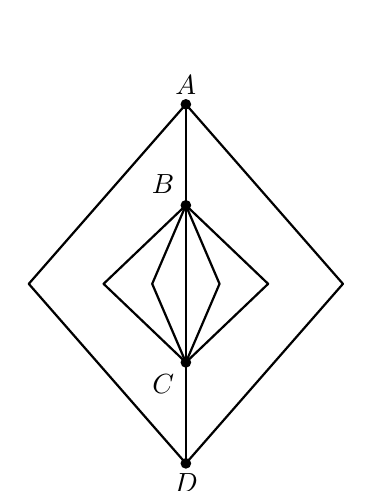
\begin{tikzpicture}[>=Stealth, scale=0.95, line cap=round, line join=round]
  % 依原書 p.178 精確繪製多層菱形歐拉圖
  \coordinate (A) at (0, 2.4);
  \coordinate (B) at (0, 1.05);
  \coordinate (C) at (0, -1.05);
  \coordinate (D) at (0, -2.4);
  \coordinate (L1) at (-2.1, 0);
  \coordinate (R1) at (2.1, 0);
  \coordinate (L2) at (-1.1, 0);
  \coordinate (R2) at (1.1, 0);
  \coordinate (L3) at (-0.45, 0);
  \coordinate (R3) at (0.45, 0);

  \draw[thick] (A) -- (L1) -- (D) -- (R1) -- cycle;
  \draw[thick] (B) -- (L2) -- (C) -- (R2) -- cycle;
  \draw[thick] (B) -- (L3) -- (C) -- (R3) -- cycle;
  \draw[thick] (A) -- (D);

  \filldraw (A) circle (1.8pt) node[above] {$A$};
  \filldraw (B) circle (1.8pt) node[above left=1pt] {$B$};
  \filldraw (C) circle (1.8pt) node[below left=1pt] {$C$};
  \filldraw (D) circle (1.8pt) node[below] {$D$};
\end{tikzpicture}
\caption{警察巡邏路線圖（歐拉圖）}
\label{fig:b6s-4-prob-patrol}
\end{figure}

\paragraph{【解答】}
$N = 6! = 720$。故 (C), (E) 為真。（第五冊，第二章）。\hfill$\#$


% ==========================================
% 附錄 IV\quad 導數 (pp. 179-214)
% ==========================================
\newpage
\phantomsection
\section*{附錄 IV\quad 導數}\label{sec:b6s-app4}
\addcontentsline{toc}{section}{\texorpdfstring{附錄 IV\quad 導數}{附錄 IV 導數}}
\resetsectcounters

\begin{itemize}[leftmargin=3em, itemsep=0.2em]
  \item[§ 1] \textbf{函數與極限}
  \item[§ 2] \textbf{導函數}
  \begin{itemize}[leftmargin=2em, itemsep=0.1em]
    \item[甲、] 變率和導數
    \item[乙、] 導函數
  \end{itemize}
  \item[§ 3] \textbf{幾個基本函數的微分}
  \begin{itemize}[leftmargin=2em, itemsep=0.1em]
    \item[甲、] 三角函數的導函數
    \item[乙、] 指數函數與對數函數
    \item[丙、] 高階導函數
  \end{itemize}
  \item[§ 4] \textbf{函數圖形}
  \begin{itemize}[leftmargin=2em, itemsep=0.1em]
    \item[甲、] 切線方程式
    \item[乙、] 極大極小
  \end{itemize}
  \item[§ 5] \textbf{近似值}
  \begin{itemize}[leftmargin=2em, itemsep=0.1em]
    \item[甲、] 均值定理與泰勒公式
    \item[乙、] 牛頓式求根法
  \end{itemize}
  \item[§ 6] \textbf{導數與面積}
\end{itemize}

\begin{center}
$* \qquad * \qquad * \qquad * \qquad *$
\end{center}

\phantomsection
\subsection*{§ 1\quad 函數與極限}\label{subsec:b6s-app4-1}
\addcontentsline{toc}{subsection}{\texorpdfstring{§ 1\quad 函數與極限}{§ 1 函數與極限}}

在第一冊第五章裡，我們討論了函數的涵義，在第二冊第二章我們又討論了數列和數列的極限，其實數列就是由自然數集合到實數集合的函數。所以，是一種函數的特例。因此，很自然地我們就可以考慮到一般函數的極限觀念。

\begin{example}\label{ex:b6s-app4-1}
令 $f: \mathbb{R}\to\mathbb{R}$ 定義如下：
\[ f(x) = 1+x \]
則它的圖形如圖 1-1。顯然，當 $x$ 不管從左或從右趨近於 0 時，$y$ 就會趨近於 1。

在這種情形，仿照數列極限的定義，我們就說當 $x$ 趨近於 0 時，函數 $f$ 的極限為 1，記作
\[ \lim_{x\to 0} f(x) = 1 \]
\end{example}

\begin{example}\label{ex:b6s-app4-2}
設函數 $f: \mathbb{R}\to\mathbb{R}$ 由下式定義：
\[ f(x) = |x-1| \]
則它的圖示如右（圖 1-2）。顯然，當 $x$ 趨近於 1 時，$y$ 趨近於 0。因此，當 $x$ 趨近於 1 時函數 $f$ 的極限為 0，$\lim_{x\to 1} f(x) = 0$。
\end{example}

\begin{figure}[H]
\centering
\begin{subfigure}[b]{0.45\textwidth}
\centering
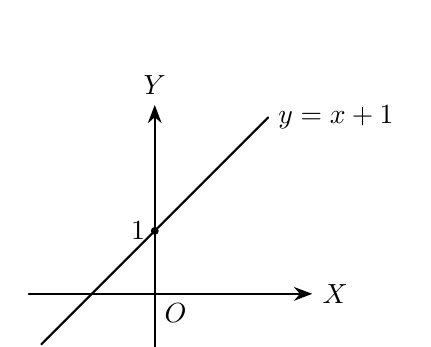
\begin{tikzpicture}[>=Stealth, scale=0.8, line cap=round]
  \draw[->, thick] (-2, 0) -- (2.5, 0) node[right] {$X$};
  \draw[->, thick] (0, -1) -- (0, 3) node[above] {$Y$};
  \node[below right] at (0, 0) {$O$};
  \draw[thick] (-1.8, -0.8) -- (1.8, 2.8) node[right] {$y=x+1$};
  \filldraw (0, 1) circle (1.5pt) node[left] {$1$};
\end{tikzpicture}
\caption{圖 1-1}
\end{subfigure}
\begin{subfigure}[b]{0.45\textwidth}
\centering
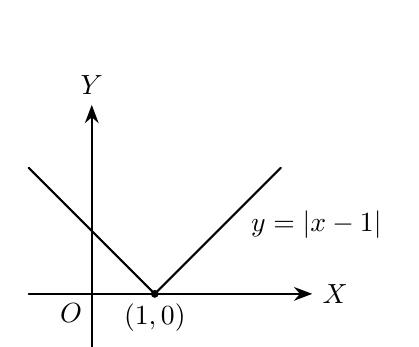
\begin{tikzpicture}[>=Stealth, scale=0.8, line cap=round]
  \draw[->, thick] (-1, 0) -- (3.5, 0) node[right] {$X$};
  \draw[->, thick] (0, -1) -- (0, 3) node[above] {$Y$};
  \node[below left] at (0, 0) {$O$};
  \draw[thick] (-1, 2) -- (1, 0) -- (3, 2);
  \node[right=4pt] at (2.2, 1.1) {$y=|x-1|$};
  \filldraw (1, 0) circle (1.5pt) node[below] {$(1,0)$};
\end{tikzpicture}
\caption{圖 1-2}
\end{subfigure}
\caption{函數極限直觀圖示}
\label{fig:b6s-app4-limit-intro}
\end{figure}

對於任意函數 $f: A\to B$，當 $x$ 趨近 $a$ 於時，$f(x)$ 趨近於 $b$，則稱 $x$ 趨近於 $a$ 時函數 $f$ 的極限為 $b$，記為 $\lim_{x\to a} f(x) = b$。

這就是說，當 $x$ 無限逼近於 $a$ 時，$f(x)$ 就會無限的逼近於 $b$。換一種方式講，就是說，對任意靠近 $b$ 的範圍內，只要 $x$ 相當接近 $a$，$f(x)$ 就會在這個 $b$ 的臨近範圍內。這些話可用數學符號表示如下：
\[ \text{對於任意的 } \varepsilon > 0, \text{ 一定存在 } \delta > 0 \text{ 使得 } |x-a| < \delta \implies |f(x)-b| < \varepsilon \]

上面這種嚴格的定義，在現階段我們不須要去強調它。我們只要接受「當 $x$ 趨近於 $a$ 時，$f(x)$ 趨近於 $b$，就說 $\lim_{x\to a} f(x) = b$」這個觀念就足夠了。

\begin{example}\label{ex:b6s-app4-3}
求 $\lim_{x\to 2} \dfrac{x^2-4}{x-2}$。
\end{example}

\paragraph{【解】}
若 $f(x) = \dfrac{x^2-4}{x-2}$，當 $x=2$ 時，我們從式中不知道 $f(2)$ 等於多少。但我們知道，對於 $x\ne 2$ 的實數，
\[ f(x) = \dfrac{x^2-4}{x-2} = x+2 \]
所以，當 $x\longrightarrow 2$ 時，$f(x)\longrightarrow 4$，因此 $\lim_{x\to 2}\dfrac{x^2-4}{x-2} = 4$。\hfill$\#$

\begin{example}\label{ex:b6s-app4-4}
求 $\lim_{x\to 0} x\sin\dfrac{1}{x}$。
\end{example}

\paragraph{【解】}
當 $x$ 趨近於 0 時，因為 $\sin\dfrac{1}{x}$ 是一週期函數 $\sin\dfrac{1}{x}$ 在 $-1$ 與 1 之間變動，但無論如何 $\left|\sin\dfrac{1}{x}\right| \le 1$，因此
\[ \left|x\sin\dfrac{1}{x}\right| \le |x| \]
所以當 $x\longrightarrow 0$ 時，$\left|x\sin\dfrac{1}{x}\right|\longrightarrow 0$，因此
\[ \lim_{x\to 0} x\sin\dfrac{1}{x} = 0 \text{。}\hfill\# \]

並不是所有的極限都會存在，下面就是一個例子。

\begin{example}\label{ex:b6s-app4-5}
求 $\lim_{x\to 0}\dfrac{|x|}{x}$。
\end{example}

\paragraph{【解】}
我們先看看 $f(x) = \dfrac{|x|}{x}$ 的圖形，當 $x>0$ 時，$|x|=x$，因此 $f(x) = 1$；當 $x<0$ 時，$|x|=-x$，所以 $f(x) = -1$。

\begin{figure}[H]
\centering
\begin{tikzpicture}[>=Stealth, scale=0.9, line cap=round]
  \draw[->, thick] (-2.5, 0) -- (2.5, 0) node[right] {$X$};
  \draw[->, thick] (0, -2) -- (0, 2) node[above] {$Y$};
  \node[below right] at (0, 0) {$O$};

  \draw[line width=1.5pt] (0.05, 1) -- (2.2, 1);
  \draw (0, 1) circle (2pt);
  \draw[line width=1.5pt] (-2.2, -1) -- (-0.05, -1);
  \draw (0, -1) circle (2pt);
\end{tikzpicture}
\caption{圖 1-3\quad 符號函數 $\dfrac{|x|}{x}$ 之跳躍不連續圖形}
\label{fig:b6s-app4-signum}
\end{figure}

其圖如圖 1-3，可見當 $x$ 從左（小於 0）趨近於 0 時，$\dfrac{|x|}{x}$ 趨近於 $-1$，而當 $x$ 從右（大於 0）趨近於 0 時，$\dfrac{|x|}{x}$ 趨近於 1。因此我們不能說：當 $x$ 趨近於 0 時，$\dfrac{|x|}{x}$ 趨近於某一固定實數，所以 $\lim_{x\to 0}\dfrac{|x|}{x}$ 不存在。\hfill$\#$

如同數列的極限一樣，函數的極限有下述的性質：如果 $f, g$ 為兩個函數，且 $\lim_{x\to a} f(x)$ 和 $\lim_{x\to a} g(x)$ 都存在，則 $\lim_{x\to a}(f(x)\pm g(x))$，$\lim_{x\to a}(f(x)g(x))$ 存在，而且：
\begin{enumerate}[label=\Roman*., leftmargin=2em]
  \item $\lim_{x\to a}(f(x)+g(x)) = \lim_{x\to a}f(x) + \lim_{x\to a}g(x)$
  \item $\lim_{x\to a}(f(x)-g(x)) = \lim_{x\to a}f(x) - \lim_{x\to a}g(x)$
  \item $\lim_{x\to a}(f(x)g(x)) = \lim_{x\to a}f(x) \cdot \lim_{x\to a}g(x)$
  \item 如果再加上條件：$\lim_{x\to a}g(x)\ne 0$，則 $\lim_{x\to a}\dfrac{f(x)}{g(x)}$ 存在，而且
  \[ \lim_{x\to a}\dfrac{f(x)}{g(x)} = \dfrac{\lim_{x\to a}f(x)}{\lim_{x\to a}g(x)} \]
  \item 如果 $\sqrt[n]{\lim_{x\to a}f(x)}$ 有意義（有定義）時，則 $\lim_{x\to a}\sqrt[n]{f(x)}$ 存在，而且
  \[ \lim_{x\to a}\sqrt[n]{f(x)} = \sqrt[n]{\lim_{x\to a}f(x)} \]
\end{enumerate}

這些性質表明了，在“良好”的情況下，函數間相加減乘數或開根號的運算可以與取極限的運算互換。

這些等式我們不做嚴密的證明，只要知道如何應用就可以了。

\begin{discussion}\label{ex:b6s-app4-disc1}\label{disc:b6s-app4-1}
令 $f(x) = a_0 + a_1 x + \dots + a_n x^n$，則
\begin{align*}
\lim_{x\to a} f(x) &= \lim_{x\to a}(a_0 + a_1 x + \dots + a_n x^n) \\
&= \lim_{x\to a}a_0 + \lim_{x\to a}a_1 x + \dots + \lim_{x\to a}a_n x^n \\
&= \lim_{x\to a}a_0 + \lim_{x\to a}a_1\lim_{x\to a}x + \dots + \lim_{x\to a}a_n\left(\lim_{x\to a}x\right)^n \\
&= a_0 + a_1 a + \dots + a_n a^n
\end{align*}
\end{discussion}

\begin{example}\label{ex:b6s-app4-6}
試求 $\lim_{x\to 2} \dfrac{x-2}{\sqrt{x^2-4}}$。
\end{example}

\paragraph{【解】}
\begin{align*}
\lim_{x\to 2} \dfrac{x-2}{\sqrt{x^2-4}} &= \lim_{x\to 2}\dfrac{(\sqrt{x-2})^2}{\sqrt{x-2}\sqrt{x+2}} = \lim_{x\to 2}\dfrac{\sqrt{x-2}}{\sqrt{x+2}} \\
&= \lim_{x\to 2}\sqrt{\dfrac{x-2}{x+2}} = 0
\end{align*}
因為 $\lim_{x\to 2}\dfrac{x-2}{x+2} = 0$。\hfill$\#$

\subsubsection*{習題 1}\label{sec:b6s-ex-app4-1}

\begin{enumerate}[label=\arabic*., leftmargin=2em]
  \item 試求下列各極限：
  \begin{multicols}{2}
  \begin{enumerate}[label=(\arabic*)]
    \item $\lim_{x\to 1}(1+x+x^2)$
    \item $\lim_{x\to 4}(1+\sqrt{x}+x^2)$
    \item $\lim_{x\to 1}\dfrac{x^3-2x^2+1}{x-1}$
    \item $\lim_{x\to 1}\dfrac{\sqrt{1-x^2}}{\sqrt{1-x}}$
    \item $\lim_{x\to 1}\dfrac{x^3-x^2-x+1}{x^2+x-2}$
    \item $\lim_{x\to 0}(\sqrt{a+x}+\sqrt{a-x})$
    \item $\lim_{x\to 0}\dfrac{x}{\sqrt{1+x}-\sqrt{1-x}}$
    \item $\lim_{x\to 1}\dfrac{x-1}{\sqrt[3]{x}-1}$
    \item $\lim_{x\to 0}x\cos\dfrac{1}{x}$
    \item $\lim_{x\to 1}\dfrac{x-1}{x}\sin\dfrac{1}{x-1}$
  \end{enumerate}
  \end{multicols}

  \item 令 $[x]$ 表示小於或等於 $x$ 的最大整數，試問
  \[ \lim_{x\to 1}[x] \text{ 是否存在？} \qquad \lim_{x\to 0.5}[x] \text{ 是否存在？} \]

  \item 將 $x$ 看做常數，試求：
  \[ \lim_{h\to 0}\dfrac{2(x+h)^2 - 5(x+h)^3 - 2x^2 - 5x^3}{h} \]

  \item 令 $f(x)=x^2$，試證 $\lim_{h\to 0}\dfrac{f(x+h)-f(x)}{h} = 2x$。

  \item 問 $a$ 為何值時，$\lim_{x\to 1}\dfrac{x^2-6x+a}{x^2+2x-3}$ 有極限？它的極限是多少？
\end{enumerate}

\phantomsection
\subsection*{§ 2\quad 導函數}\label{subsec:b6s-app4-2}
\addcontentsline{toc}{subsection}{\texorpdfstring{§ 2\quad 導函數}{§ 2 導函數}}
\setcounter{theorem}{0}
\renewcommand{\thetheorem}{2.\arabic{theorem}}

\subsubsection*{甲、變率和導數}

數學上，我們用函數來描示事物的狀態和幾何圖形，對於事物的狀態和幾何圖形我們常須了解它的變動情形。

下表是縱貫鐵路光華號 2001 次列車所停各站的時刻和該站與基隆的距離：

\begin{center}
\textbf{表 2-1}

\renewcommand{\arraystretch}{1.2}
\begin{tabular}{|c|c|c|c|c|c|c|}
\hline
站名 & 基隆 & 臺北 & 臺中 & 臺南 & 高雄 & 屏東 \\ \hline
時間 & 6.17 & 7.00 & 9.32 & 11.28 & 12.10 & 12.34 \\ \hline
距離 & 0 & 28.6 & 197.4 & 357.5 & 404.2 & 425.1 \\ \hline
\end{tabular}
\end{center}

現在以 $x$ 代表時間，$y=f(x)$ 表示在時間為 $x$ 時，該列車與基隆的距離則由表記：
\begin{align*}
f(7.00) &= 28.6 \qquad (\text{在臺北站}) \\
f(9.32) &= 197.4 \qquad (\text{在臺中站}) \\
&\ \ \vdots \\
f(12.34) &= 425.1 \qquad (\text{在屏東站})
\end{align*}
注意上面的 $x$ 值並非十進位數！函數 $f$ 描述了該列車行駛狀態，由 $f$，我們知道該列，從基隆到屏東所須時間為 6.28 小時（$\doteq 6$ 小時 17 分）所以，它平均每小時走 $\dfrac{425.1}{6.28} = 67.69$ 公里，我們說這是它的平均速率，在數學上，我們稱它為\textbf{平均變率}。

當函數 $y=f(x)$ 在線段 $[a, b] = \{x; a\le x\le b\}$ 上定義時，比值 $\dfrac{f(b)-f(a)}{b-a}$ 叫做函數 $y=f(x)$ 在 $a, b$ 間的平均變率。如下圖所示，平均變率，其實就是線段 $\overline{P_a P_b}$ 的斜率。

\begin{figure}[H]
\centering
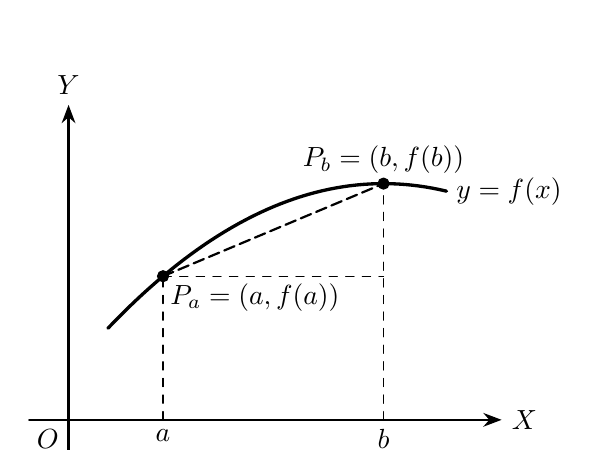
\begin{tikzpicture}[>=Stealth, scale=1.0, line cap=round, line join=round]
  \draw[->, thick] (-0.5, 0) -- (5.5, 0) node[right] {$X$};
  \draw[->, thick] (0, -0.5) -- (0, 4.0) node[above] {$Y$};
  \node[below left] at (0, 0) {$O$};

  % 曲線 y = f(x)
  \draw[line width=1.2pt, domain=0.5:4.8, samples=50] plot (\x, {0.6 + 1.2*\x - 0.15*\x*\x});
  \node[right] at (4.8, 2.9) {$y=f(x)$};

  \coordinate (Pa) at (1.2, 1.824);
  \coordinate (Pb) at (4.0, 3.0);

  \draw[thick, dash pattern=on 4pt off 2pt] (Pa) -- (Pb);
  \draw[dashed] (1.2, 0) node[below] {$a$} -- (Pa);
  \draw[dashed] (4.0, 0) node[below] {$b$} -- (Pb);
  \draw[dashed] (Pa) -- (4.0, 1.824);

  \filldraw (Pa) circle (2pt) node[below right=2pt, fill=white, inner sep=1pt] {$P_a=(a, f(a))$};
  \filldraw (Pb) circle (2pt) node[above] {$P_b=(b, f(b))$};
\end{tikzpicture}
\caption{圖 2-1\quad 平均變率之幾何意義（割線斜率）}
\label{fig:b6s-app4-avg-rate}
\end{figure}

對於等速運動來說，取任意時間內的平均速率都相等。但對上例的火車來說，平均速率並不能代表該列車在任意時刻走的快慢。這很容易從表中驗算比較得來。

\subsubsection*{作業 1}
試計算下列各站間，2001 次光華號的平均速率：
\begin{enumerate}[label=\alph*., leftmargin=2em]
  \item 臺北與臺南間
  \item 臺中與高雄間
\end{enumerate}

物理學告訴我們，要看一物體運動的快慢，必需用每瞬間的快慢來衡量，如以光華號車為例，該車在 10 時正行駛快慢的程度，應以 10 時到 10 時 01 分所走的路程，或甚至更短時間 $\Delta t$ 所走的路程的平均速率才能表示它的快慢，而且 $\Delta t$ 越逼近於 0 的平均速率越能表示該時刻的速率，以此推之於函數的變動情形，我們有如下的觀念：

\begin{definition*}[導數（變率）的定義]\label{def:b6s-app4-derivative}
對於一個固定的 $a$，假如平均變率 $\dfrac{f(b)-f(a)}{b-a}$ 在 $b\to a$ 時有一個極限值，即 $\lim_{b\to a}\dfrac{f(b)-f(a)}{b-a}$ 存在，則稱這種極限為 $y=f(x)$ 在 $x=a$ 時的\textbf{瞬間變率}又稱為函數 $f(x)$ 在 $x=a$ 的\textbf{導數}。
\end{definition*}

平常為了明示 $a$ 為固定，而 $b\to a$，我們改用 $b=a+h$（即 $h=b-a$）則 $y=f(x)$ 在 $x=a$ 的導數為
\[ \lim_{h\to 0}\dfrac{f(a+h)-f(a)}{h} \]
我們將 $f(x)$ 在 $x=a$ 的導數記為 $\left.\dfrac{df}{dx}\right|_a$，又記為 $f'(a)$。

\paragraph{注意：}
\begin{enumerate}[label=(\roman*), leftmargin=2em]
  \item $h$ 是可正可負的。
  \item 當上述極限不存在時，我們說 $y=f(x)$ 在點 $x=a$ 無導數。
  \item 由上節所定義的極限觀念，不難看出函數 $f$ 在 $x=a$ 連續的充分必要條件為 $\lim_{x\to a}f(x) = f(a)$。如果 $f$ 在 $x=a$ 有導數 $f'(a)$，則
  \begin{align*}
  \lim_{x\to a}[f(x)-f(a)] &= \lim_{x\to a}\left[\dfrac{f(x)-f(a)}{x-a}(x-a)\right] \\
  &= \lim_{x\to a}\dfrac{f(x)-f(a)}{x-a}\lim_{x\to a}(x-a) = 0
  \end{align*}
  所以 $f$ 在 $x=a$ 連續。
\end{enumerate}

這種求函數在某點的導數的手段叫做\textbf{微分}。函數 $f(x)$ 在 $x=a$ 有導數時，稱 $f(x)$ 在 $x=a$ 可微分或可微又可說 $f(x)$ 在 $x=a$ 處是平滑的，否則稱為在 $x=a$ 不可微分或不可微。

\begin{example}\label{ex:b6s-app4-7}
求 $f(x)=cx+d$ 在 $x=a$ 的導數。
\end{example}

\paragraph{【解】}
\[ f'(a) = \lim_{h\to 0}\dfrac{f(a+h)-f(a)}{h} = \lim_{h\to 0}\dfrac{[c(a+h)+d]-[ca+d]}{h} = c \]
所以 $f(x)=cx+d$，在任意點 $x=a$ 的導數都為常數 $c$。這由 $y=f(x)$ 的圖形很容易看出來，因為它的圖形是直線，所以圖上任意兩點連線的斜率為常數。\hfill$\#$

\begin{example}\label{ex:b6s-app4-8}
試求 $y=x^2$ 在 $x=a$ 時的導數。
\end{example}

\paragraph{【解】}
因為 $f(a+h) = (a+h)^2 = a^2+2ah+h^2$，$f(a+h)-f(a) = 2ah+h^2$。
所以 $f'(a) = \lim_{h\to 0}\dfrac{2ah+h^2}{h} = 2a$。\hfill$\#$

\begin{example}\label{ex:b6s-app4-9}
試求 $y=x^n$ 在 $x=a$ 時的導數。
\end{example}

\paragraph{【解】}
\begin{align*}
f'(a) &= \lim_{h\to 0}\dfrac{(a+h)^n - a^n}{h} = \lim_{h\to 0}\dfrac{na^{n-1}h + {}_n C_2 a^{n-2}h^2 + \dots + h^n}{h} \quad (\text{二項式定理展開}) \\
&= na^{n-1} \text{。}\hfill\#
\end{align*}

\begin{example}\label{ex:b6s-app4-10}
設 $f(x)=|x|$，求 $f(x)$ 在 $x=0$ 的導數。
\end{example}

\paragraph{【解】}
當 $h>0$ 時，$\dfrac{f(0+h)-f(0)}{h} = \dfrac{h}{h} = 1$；故當 $h$ 從右邊（大於 0）趨近於 0 時，$\dfrac{f(0+h)-f(0)}{h}$ 趨近於 1。
當 $h<0$ 時，$\dfrac{f(0+h)-f(0)}{h} = -1$，故當 $h$ 從左（小於 0）趨近於 0 時，$\dfrac{f(0+h)-f(0)}{h}$ 趨近於 $-1$。所以當 $h$ 趨近於 0 時，$\dfrac{f(0+h)-f(0)}{h}$ 不能趨近於一固定數，就是說 $\lim_{h\to 0}\dfrac{f(0+h)-f(0)}{h}$ 不存在。所以 $f(x)=|x|$ 在 $x=0$ 無導數。\hfill$\#$

\begin{figure}[H]
\centering
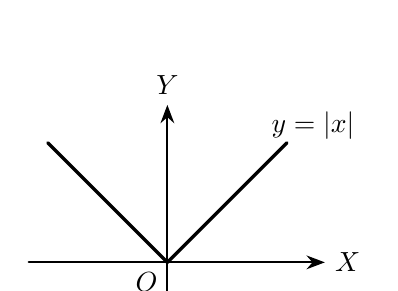
\begin{tikzpicture}[>=Stealth, scale=0.8, line cap=round, line join=round]
  \draw[->, thick] (-2.2, 0) -- (2.5, 0) node[right] {$X$};
  \draw[->, thick] (0, -0.6) -- (0, 2.5) node[above] {$Y$};
  \node[below left] at (0, 0) {$O$};
  \draw[line width=1.2pt] (-1.9, 1.9) -- (0, 0) -- (1.9, 1.9);
  \node[above right] at (1.5, 1.8) {$y=|x|$};
\end{tikzpicture}
\end{figure}

\begin{example}\label{ex:b6s-app4-11}
令 $x\ge 0, f(x)=\sqrt{x}$，試求 $f(x)$ 在 $x=a\ (>0)$ 時的導數。
\end{example}

\paragraph{【解】}
對任意 $x=a>0$，取 $|h|$ 相當小時，$a+h>0$，所以 $\sqrt{a+h}$ 有意義，而且
\[ \dfrac{\sqrt{a+h}-\sqrt{a}}{h} = \dfrac{a+h-a}{h(\sqrt{a+h}+\sqrt{a})} = \dfrac{1}{\sqrt{a+h}+\sqrt{a}} \]
所以 $f'(a) = \lim_{h\to 0}\dfrac{f(a+h)-f(a)}{h} = \lim_{h\to 0}\dfrac{1}{\sqrt{a+h}+\sqrt{a}} = \dfrac{1}{2\sqrt{a}}$。\hfill$\#$

\subsubsection*{作業 2}
當 $x=0$ 時，$f(x)=\sqrt{x}$ 的導數為何？有無意義？

\subsubsection*{習題 2-A}\label{sec:b6s-ex-app4-2a}

\begin{enumerate}[label=\arabic*., leftmargin=2em]
  \item 試求下列各函數在 $x=a$ 時的導數：
  \begin{multicols}{2}
  \begin{enumerate}[label=(\roman*)]
    \item $f(x)=3x+2$
    \item $f(x)=6x^2+7$
    \item $f(x)=a_0+a_1 x+\dots+a_n x^n$
    \item $f(x)=\dfrac{1}{x}, x\ne 0$
    \item $f(x)=\sqrt{3x+1}, x>-\frac{1}{3}$
  \end{enumerate}
  \end{multicols}

  \item 下列各函數在何時才有意義？才有導數？
  \begin{multicols}{2}
  \begin{enumerate}[label=(\roman*)]
    \item $f(x)=\dfrac{1}{2x+1}$
    \item $f(x)=\sqrt{x-1}$
    \item $f(x)=\sqrt{|x|}$
    \item $f(x)=\sqrt{x^2-1}$
    \item $f(x)=\sqrt[3]{x}$
    \item $f(x)=x^{\frac{1}{m}}$
    \item $f(x)=\sqrt{ax+b}$
  \end{enumerate}
  \end{multicols}

  \item 如圖，一石頭沿一 $45^\circ$ 的斜坡滾下，若石頭在斜坡滾下的距離為 $y$ 時，它在垂直方向下降的高度為 $x$，現 $x$ 為時間 $t$ 的函數 $x(t) = \dfrac{1}{2}gt^2, g=980\text{ cm/t}^2$。試問：a. 石頭的垂直下降速率；b. 石頭沿山坡滾動速率。
  \begin{center}
  \begin{tikzpicture}[>=Stealth, scale=0.85, line cap=round, line join=round]
    \draw[thick] (0, 0) -- (4.2, 0);
    \draw[thick] (0, 0) -- (2.9, 2.9);
    \draw[thin] (0.65, 0) arc (0:45:0.65);
    \node[font=\footnotesize] at (1.05, 0.28) {$45^\circ$};
    % 石頭與位移箭頭
    \draw[thick, fill=white] (2.45, 2.65) circle (0.18);
    \draw[->, thick] (2.35, 2.50) -- (1.15, 1.30);
    \node[below right, font=\footnotesize] at (1.75, 1.85) {$y$};
    % 垂直高度 x 虛線直角三角形
    \draw[dashed] (1.15, 1.15) -- (2.6, 1.15) -- (2.6, 2.6);
    \node[right, font=\footnotesize] at (2.6, 1.85) {$x$};
  \end{tikzpicture}
  \end{center}
\end{enumerate}

\subsubsection*{乙、導函數}

當函數 $y=f(x)$ 到處都可微時，對應：
\[ x \longrightarrow f'(x) = \lim_{h\to 0}\dfrac{f(x+h)-f(x)}{h} \]
就成為一新函數，這新函數稱為 $y=f(x)$ 的\textbf{導函數}，通常以 $y'=f'(x)$ 或 $\dfrac{dy}{dx} = \dfrac{df(x)}{dx}$ 表之。

\begin{align*}
\text{〔例 7〕}\quad f(x)=cx+d \text{ 的導函數為 } y' &= c \\
\text{〔例 8〕}\quad f(x)=x^2 \text{ 的導函數為 } y' &= 2x \\
\text{〔例 9〕}\quad y=x^n \text{ 的導函數為 } y' &= nx^{n-1} \\
\text{〔例 10〕}\quad y=|x| \text{ 的導函數為 } y' &= \begin{cases} 1 & \text{當 } x>0 \\ -1 & \text{當 } x<0 \end{cases} \quad \text{當 } x=0 \text{ 時 } y' \text{ 無定義。} \\
\text{〔例 11〕}\quad y=\sqrt{x} \text{ 的導函數為 } y' &= \dfrac{1}{2\sqrt{x}}, \quad x>0
\end{align*}

由一個已知函數求出它的導函數的「運算」也叫做微分，下面我們來談一談微分這個新的運算和我們原來就熟悉函數間的運算如「加」，「減」，「乘」，「除」等的關係。

\begin{theorem}[微分運算的基本法則]\label{thm:b6s-app4-diff-rules}
令函數 $f(x), g(x)$ 為到處可微，則
\begin{enumerate}[label=(\roman*), leftmargin=2em]
  \item $\dfrac{d}{dx}(f(x)\pm g(x)) = \dfrac{df(x)}{dx} \pm \dfrac{dg(x)}{dx}$；
  \item $\dfrac{d}{dx}(f(x)g(x)) = \dfrac{df(x)}{dx}g(x) + f(x)\dfrac{dg(x)}{dx}$；
  \item $\dfrac{d}{dx}\left(\dfrac{f(x)}{g(x)}\right) = \dfrac{\dfrac{df(x)}{dx}g(x) - f(x)\dfrac{dg(x)}{dx}}{(g(x))^2}, \qquad (g(x)\ne 0)$；
  \item 若 $y=f(u), u=g(x)$ 即 $y=f(g(x))$ 為 $f, g$ 的合成函數，則
  \[ \dfrac{d}{dx}[f(g(x))] = \left[\dfrac{df(u)}{du}\right]\dfrac{dg(x)}{dx} \]
\end{enumerate}
\end{theorem}

\begin{proof}[【證明】]
(i), (ii) 直接由極限的性質而來，現在證明 (iii)：
\begin{align*}
\dfrac{d}{dx}\left(\dfrac{1}{g(x)}\right) &= \lim_{h\to 0}\dfrac{\dfrac{1}{g(x+h)} - \dfrac{1}{g(x)}}{h} = \lim_{h\to 0}\dfrac{-[g(x+h)-g(x)]}{h g(x+h)g(x)} \\
&= -\lim_{h\to 0}\dfrac{g(x+h)-g(x)}{h}\cdot\lim_{h\to 0}\dfrac{1}{g(x+h)g(x)} \\
&= -\dfrac{dg(x)}{dx}\cdot\dfrac{1}{[g(x)]^2}
\end{align*}
再由 (ii) 得
\begin{align*}
\dfrac{d}{dx}\left(\dfrac{f(x)}{g(x)}\right) &= \dfrac{df(x)}{dx}\cdot\dfrac{1}{g(x)} + f(x)\dfrac{d\left(\dfrac{1}{g(x)}\right)}{dx} \\
&= \dfrac{\dfrac{df(x)}{dx}g(x) - f(x)\dfrac{dg(x)}{dx}}{[g(x)]^2}
\end{align*}
(iv) 令 $k=g(x+h)-g(x)$，則 $g(x+h)=u+k$，而且當 $h\longrightarrow 0$ 時，$k\longrightarrow 0$，所以：
\begin{align*}
\dfrac{d}{dx}[f(g(x))] &= \lim_{h\to 0}\dfrac{f(g(x+h))-f(g(x))}{h} \\
&= \lim_{h\to 0}\left[\dfrac{f(u+k)-f(u)}{k}\cdot\dfrac{k}{h}\right] \\
&= \lim_{k\to 0}\dfrac{f(u+k)-f(u)}{k}\cdot\lim_{h\to 0}\dfrac{g(x+h)-g(x)}{h} \\
&= \dfrac{df(u)}{du}\cdot\dfrac{dg(x)}{dx}
\end{align*}
\end{proof}\hfill$\#$

上述諸式是計算函數不可或缺的工具，但這裡須注意公式 (iv) 並不是對一切函數都成立，這裡所說的條件並不完整，這裡的“證明”也不是一個完全的“證明”。這些精密的證明和條件我們不在這裡敘述，而留到大學正式微積分課作詳細證明。

\begin{example}\label{ex:b6s-app4-12}
$y=(2x+1)^2$ 可以看做 $y=u^2, u=2x+1$ 的合成函數，所以由 (iv) 得
\[ y' = \dfrac{dy}{du}\cdot\dfrac{du}{dx} = 2u \cdot 2 = 4(2x+1) \text{。}\hfill\# \]
\end{example}

\begin{example}\label{ex:b6s-app4-13}
$y=\sqrt{3x+1}, 3x+1>0$，試求 $y'$。
\end{example}

\paragraph{【解】}
令 $u=3x+1$，則 $y=\sqrt{u}$，故
\[ y' = \dfrac{d\sqrt{u}}{du}\cdot\dfrac{du}{dx} = \dfrac{1}{2\sqrt{u}}\cdot 3 = \dfrac{3}{2\sqrt{3x+1}} \text{。}\hfill\# \]

\subsubsection*{習題 2-B}\label{sec:b6s-ex-app4-2b}

試計算下列各式之導函數：
\begin{multicols}{2}
\begin{enumerate}[label=\arabic*., leftmargin=2em]
  \item $y = 3x^2$
  \item $y = 5x^3+4x^2+3x+2$
  \item $y = (3x^3+2x^2+x+1)^2$
  \item $y = (2x^2+1)(3x+2)$
  \item $y = \sqrt{2x-1}, (2x>1)$
  \item $y = \dfrac{1}{x^4}, (x\ne 0)$
  \item $y = \dfrac{1}{\sqrt{x+1}}, (x>-1)$
  \item $y = \sqrt{2x^2+3x+1}$
  \item $y = \left(\dfrac{2x+5}{3x+1}\right)^2$
  \item $y = (2x^2+4x-1)\sqrt{x^2+1}$
\end{enumerate}
\end{multicols}

\phantomsection
\subsection*{*§ 3\quad 幾個基本函數的微分}\label{subsec:b6s-app4-3}
\addcontentsline{toc}{subsection}{\texorpdfstring{*§ 3\quad 幾個基本函數的微分}{*§ 3 幾個基本函數的微分}}
\setcounter{lemma}{0}
\renewcommand{\thelemma}{3.\arabic{lemma}}
\setcounter{theorem}{1}
\renewcommand{\thetheorem}{3.\arabic{theorem}}

多項式，三角函數，和指數是我們常見而且應用最廣的幾種函數。上節例 9 和定理 2.1 已告訴我們多項式 $f(x)=a_0+a_1 x+\dots+a_n x^n$ 的導數為 $f'(x)=a_1+2a_2 x+\dots+n a_n x^{n-1}$。在這節裡我們來求三角函數和指數函數的導函數。

\subsubsection*{甲、三角函數的導函數}

我們先求 $y=\sin x$ 的導函數。要求 $y=\sin x$ 的導函數，必須利用下述的極限：

\begin{lemma}\label{lem:b6s-app4-sin-limit}
\[ \lim_{h\to 0}\dfrac{\sin h}{h} = 1 \]
\end{lemma}

\begin{figure}[H]
\centering
\begin{tikzpicture}[>=Stealth, scale=1.25, line cap=round, line join=round]
  \coordinate (O) at (0, 0);
  \draw[->, thick] (-2.1, 0) -- (2.9, 0) node[right] {$X$};
  \draw[->, thick] (0, -2.1) -- (0, 2.3) node[above] {$Y$};
  \node[below left] at (O) {$O$};

  % 完整單位圓 (與原書 p.192 一致，半徑 1.8，角度 40 度使 B' 與 A 清晰分離)
  \draw[thick] (O) circle (1.8);
  \coordinate (B) at (40:1.8);
  \coordinate (A) at (1.8, 0);
  \coordinate (Aprime) at (1.8, {1.8*tan(40)});
  \coordinate (Bprime) at ({1.8*cos(40)}, 0);

  \draw[thick] (O) -- (Aprime);
  \draw[thick] (A) -- (Aprime);
  \draw[thick] (B) -- (Bprime);

  \node[above=2pt] at (B) {$B$};
  \node[below right=1pt] at (A) {$A$};
  \node[above right=1pt] at (Aprime) {$A'$};
  \node[below=2pt] at (Bprime) {$B'$};

  \draw[thin] (0.52, 0) arc (0:40:0.52);
  \node[font=\footnotesize] at (0.68, 0.22) {$h$};
  \node[below=2pt, font=\footnotesize] at (0.56, 0) {$\cos h$};
  \node[left=1pt, font=\footnotesize] at ({1.8*cos(40)}, 0.56) {$\sin h$};
  \node[right=2pt, font=\footnotesize] at (1.8, 0.72) {$\tan h$};
\end{tikzpicture}
\caption{圖 3-1\quad $\lim_{h\to 0}\dfrac{\sin h}{h}=1$ 之單位圓幾何證明}
\label{fig:b6s-app4-sin-geom}
\end{figure}

\begin{proof}[【證明】]
參考圖 3-1，令圓 $O$ 為單位圓，則因為 $\triangle OBB' \subseteq \text{扇形 } OAB \subseteq \triangle OAA'$，而且
\begin{align*}
\triangle OBB' \text{ 的面積} &= \dfrac{1}{2}\sin h \cos h, \qquad \text{扇形 } OAB \text{ 的面積} = \dfrac{1}{2}\cdot 1 \cdot h, \\
\triangle OAA' \text{ 的面積} &= \dfrac{1}{2}\cdot 1 \cdot \tan h
\end{align*}
所以 $\sin h \cos h \le h \le \tan h$ 即 $\cos h \le \dfrac{\sin h}{h} \le \dfrac{1}{\cos h}$，所以當 $h\longrightarrow 0$ 時，$\cos h\longrightarrow 1, \dfrac{1}{\cos h}\longrightarrow 1$，故 $\lim_{h\to 0}\dfrac{\sin h}{h} = 1$。
\end{proof}\hfill$\#$

\begin{theorem}\label{thm:b6s-app4-deriv-sin}
\[ \dfrac{d}{dx}(\sin x) = \cos x \tag{I} \]
\end{theorem}

\begin{proof}[【證明】]
\begin{align*}
\dfrac{d}{dx}\sin x &= \lim_{h\to 0}\dfrac{\sin(x+h)-\sin x}{h} \\
&= \lim_{h\to 0}\dfrac{\sin x\cos h + \sin h\cos x - \sin x}{h} \\
&= \lim_{h\to 0}\left[\dfrac{\sin x(\cos h - 1)}{h} + \dfrac{\sin h}{h}\cos x\right] \\
&= \left(\lim_{h\to 0}\dfrac{\cos h - 1}{h}\right)\sin x + \left(\lim_{h\to 0}\dfrac{\sin h}{h}\right)\cos x = \cos x
\end{align*}
因為 $\lim_{h\to 0}\dfrac{\cos h - 1}{h} = \lim_{h\to 0}\dfrac{-2\sin^2\frac{h}{2}}{h} = \lim_{h\to 0}\left(-\sin\dfrac{h}{2}\right)\lim_{h\to 0}\dfrac{\sin\frac{h}{2}}{\frac{h}{2}} = 0$。
\end{proof}\hfill$\#$

應用 $\sin x$ 的導函數和上節所得的公式，我們已經可以求得其它三角函數的導函數：

\begin{theorem}\label{thm:b6s-app4-deriv-trig-other}
\begin{align*}
\dfrac{d}{dx}\cos x &= -\sin x \tag{II} \\
\dfrac{d}{dx}\tan x &= \sec^2 x \tag{III}
\end{align*}
\end{theorem}

\begin{proof}[【證明】]
(II) $\dfrac{d}{dx}\cos x = \dfrac{d}{dx}\sin\left(\dfrac{\pi}{2}+x\right) = \dfrac{d}{du}\sin u\cdot\dfrac{du}{dx}, \quad u=\dfrac{\pi}{2}+x$
\[ = \cos\left(\dfrac{\pi}{2}+x\right) = -\sin x \]
(III) $\dfrac{d}{dx}\tan x = \dfrac{d}{dx}\left(\dfrac{\sin x}{\cos x}\right) = \dfrac{\dfrac{d\sin x}{dx}\cos x - \sin x\dfrac{d\cos x}{dx}}{\cos^2 x} \quad (\text{定理 2.1, (iii)})$
\[ = \dfrac{\cos^2 x + \sin^2 x}{\cos^2 x} = \sec^2 x \quad (\text{(I), (II)}) \]
\end{proof}\hfill$\#$

\subsubsection*{乙、指數函數與對數函數的微分}

如果有家銀行的年利率是 $100\%$，存一元在該銀行一年後本利和為 $1+1=2$ 元。如果以複利計算每半年算一次，則一年後的本利率為 $\left(1+\frac{1}{2}\right)^2$ 元，每年算三次則為 $\left(1+\frac{1}{3}\right)^3$ 元，每年算 $n$ 次，則一年的本利和為 $\left(1+\frac{1}{n}\right)^n$ 元。當然 $n$ 增大時，其本利和也就增大，當 $n$ 無限的增大時，則其本利和是否會無限的增大？這就是說極限 $\lim_{n\to\infty}\left(1+\frac{1}{n}\right)^n$ 是否存在？答案是肯定的，這個極限在描寫自然現象上很重要，我們叫它尤拉數（Euler number）記為 $e$，以 $e$ 為底的對數就叫做\textbf{自然對數}。

\begin{theorem}\label{thm:b6s-app4-euler-e}
$e = \lim_{n\to\infty}\left(1+\dfrac{1}{n}\right)^n$ 存在。
\end{theorem}

\begin{proof}[【證明】]
a: $\left(1+\dfrac{1}{n}\right)^n$ 有上界，即有一 $c>0, \left(1+\dfrac{1}{n}\right)^n \le c$。因為由二項式定理知
\begin{align*}
\left(1+\dfrac{1}{n}\right)^n &= 1 + n\cdot\dfrac{1}{n} + \dfrac{n(n-1)}{2!}\left(\dfrac{1}{n}\right)^2 + \dots + \left(\dfrac{1}{n}\right)^n \\
&= 1 + 1 + \dfrac{1}{2!}\left(1-\dfrac{1}{n}\right) + \dots + \dfrac{1}{n!}\left(1-\dfrac{1}{n}\right)\dots\left(1-\dfrac{n-1}{n}\right) \\
&\le 1 + 1 + \dfrac{1}{2!} + \dots + \dfrac{1}{n!}
\end{align*}
但當 $n\ge 2$ 時，$n!\ge 2^{n-1}$，故 $\dfrac{1}{n!}\le\dfrac{1}{2^{n-1}}$，所以
\[ \left(1+\dfrac{1}{n}\right)^n \le 1 + 1 + \dfrac{1}{2} + \dfrac{1}{2^2} + \dots + \dfrac{1}{2^{n-1}} \le 3 \]
b: 數列 $a_n = \left(1+\dfrac{1}{n}\right)^n, n=1, 2, 3, \dots$ 為遞增數列，這由上面複利計算的例子很容易了解，$n+1>n$，所以 $\dfrac{1}{n}>\dfrac{1}{n+1}$，故 $\dfrac{k}{n}>\dfrac{k}{n+1}, k>0$，因此 $a_n \le a_{n+1}$。

由 a, b 和實數完備性（第二冊第三章 § 3-2），我們知道一遞增數列有上限時，它的極限 $e = \lim_{n\to\infty}\left(1+\dfrac{1}{n}\right)^n$ 存在。$e$ 的數值約等於 $2.71828182845904523536\dots$。
\end{proof}\hfill$\#$

令 $x=\dfrac{1}{h}$，則在 $h$ 從右邊（大於 0）趨近於 0 時，$x\longrightarrow\infty$。所以直觀上，我們有

\begin{theorem}\label{thm:b6s-app4-lim-h-e}
$\lim_{h\to 0}(1+h)^{\frac{1}{h}} = e$。
\end{theorem}

上面所敘述的並不是嚴格的證明，這些證明已經超過本書的範圍，在這裡不加以討論。以 $e$ 為底的對數我們叫它做自然對數，通常我們將 $\log_e x$ 記為 $\ln x$。

\setcounter{lemma}{5}
\begin{lemma}\label{lem:b6s-app4-e-limits}
\begin{enumerate}[label=(\roman*), leftmargin=2em]
  \item $\lim_{x\to 0}\dfrac{\ln(1+x)}{x} = 1$
  \item $\lim_{x\to 0}\dfrac{e^x-1}{x} = 1$
\end{enumerate}
\end{lemma}

\begin{proof}[【證明】]
(i) $\lim_{x\to 0}\dfrac{\ln(1+x)}{x} = \lim_{x\to 0}\ln(1+x)^{\frac{1}{x}} = \ln\lim_{x\to 0}(1+x)^{\frac{1}{x}} = \ln e = 1$。

(ii) 令 $e^x = 1+h$，則 $x=\ln(1+h)$，而且 $x\longrightarrow 0, h\longrightarrow 0$，故
\[ \lim_{x\to 0}\dfrac{e^x-1}{x} = \lim_{h\to 0}\dfrac{h}{\ln(1+h)} = \dfrac{1}{\lim_{h\to 0}\dfrac{\ln(1+h)}{h}} = 1 \]
\end{proof}\hfill$\#$

\setcounter{theorem}{6}
\begin{theorem}\label{thm:b6s-app4-deriv-exp-ln}
\begin{enumerate}[label=(\roman*), leftmargin=2em]
  \item $\dfrac{d}{dx}e^x = e^x$，
  \item $\dfrac{d}{dx}\ln x = \dfrac{1}{x}$
\end{enumerate}
\end{theorem}

\begin{proof}[【證明】]
(i) $\dfrac{d}{dx}e^x = \lim_{h\to 0}\dfrac{e^{x+h}-e^x}{h} = \lim_{h\to 0}\dfrac{e^x(e^h-1)}{h} = e^x\lim_{h\to 0}\dfrac{e^h-1}{h} = e^x$（引理 3.6(ii)）。

(ii) $\dfrac{d}{dx}\ln x = \lim_{h\to 0}\dfrac{\ln(x+h)-\ln x}{h} = \lim_{h\to 0}\dfrac{\ln\left(1+\frac{h}{x}\right)}{h}$。令 $t=\dfrac{h}{x}$，則 $h\longrightarrow 0$ 時，$t\longrightarrow 0$，
\[ \dfrac{d}{dx}\ln x = \lim_{h\to 0}\dfrac{1}{x}\dfrac{\ln\left(1+\frac{h}{x}\right)}{\frac{h}{x}} = \dfrac{1}{x}\lim_{t\to 0}\dfrac{\ln(1+t)}{t} = \dfrac{1}{x} \quad (\text{引理 3.6, (i)}) \]
\end{proof}\hfill$\#$

\begin{example}\label{ex:b6s-app4-14}
$a>0$，試求 $\dfrac{d}{dx} a^x$。
\end{example}

\paragraph{【解】}
$a^x = e^{x\ln a}$，故令 $u=x\ln a$，則 $\dfrac{d}{dx}a^x = \dfrac{d}{dx}e^{x\ln a} = \dfrac{d}{du}e^u \cdot \dfrac{d}{dx}(x\ln a) = (\ln a)e^u = (\ln a)e^{x\ln a} = (\ln a)a^x$。\hfill$\#$

\subsubsection*{丙、高階函數}

給一導函數 $f'(x)$，如果它的導函數存在，則稱為 $f(x)$ 的\textbf{第二階導函數}，並記之為 $f''(x)$，或寫成 $y'', \dfrac{d^2 y}{dx^2}, \dfrac{d^2}{dx^2}f(x)$。

\begin{example}\label{ex:b6s-app4-15}
求 $f(x)=3x^2+5x-2$ 的第二階導函數。
\end{example}

\paragraph{【解】}
因 $f'(x)=6x+5$，所以 $f''(x)=6$。\hfill$\#$

\begin{example}\label{ex:b6s-app4-16}
$f(x)=\sin x$ 的導函數為 $f'(x)=\cos x$，故其第二階導函數為 $f''(x)=-\sin x$。\hfill$\#$
\end{example}

依此類推，函數經過 $n$ 次微分之後，所得的函數叫做第 $n$ 階導函數，我們將它記為：$f^{(n)}(x), y^{(n)}, \dfrac{d^n}{dx^n}f(x)$ 或 $\dfrac{d^n y}{dx^n}$。

\begin{example}\label{ex:b6s-app4-17}
求 $y=x^n$ 的第 $n$ 階導函數。
\end{example}

\paragraph{【解】}
$\dfrac{dy}{dx} = nx^{n-1}, \dfrac{d^2 y}{dx^2} = n(n-1)x^{n-2}, \dots, \dfrac{d^n y}{dx^n} = n!$。\hfill$\#$

\subsubsection*{習題 3}\label{sec:b6s-ex-app4-3}

\begin{enumerate}[label=\Roman*., leftmargin=2em]
  \item 試求下列各函數的導函數：
  \begin{multicols}{2}
  \begin{enumerate}[label=\arabic*.]
    \item $x\sin x$
    \item $2x^2\sin x$
    \item $\sin x\cos x$
    \item $\dfrac{\sin x}{x}$
    \item $e^{-x}$
    \item $\dfrac{e^x}{x}$
    \item $x\ln x - x$
    \item $\log_{10} x$
    \item $e^x \ln x$
    \item $\ln(x^2+x+1)$
    \item $\ln\sqrt{1+x^2}$
    \item $\ln\sqrt{\dfrac{1+x}{1-x}}$
    \item $e^{-x}\sin(2x+1)$
    \item $e^x\sin^3 x$
    \item $a^{x^2}$
  \end{enumerate}
  \end{multicols}

  \item 試求習題 I 中各函數的第二階導函數。

  \item \textbf{簡諧運動}（如圖）：一質點沿一單位圓圓周作順時針等速圓周運動，即在時間 $t$ 時，其所掃過的角度為 $\theta(t)=\omega t$，$\omega$ 為常數。試問其在 $x$ 軸和 $y$ 軸上的投影的速率是多少？
  \begin{center}
  \begin{tikzpicture}[>=Stealth, scale=0.95, line cap=round, line join=round]
    \draw[->, thick] (-2.1, 0) -- (2.3, 0) node[right] {$X$};
    \draw[->, thick] (0, -2.0) -- (0, 2.2) node[above] {$Y$};
    \node[below left] at (0, 0) {$O$};
    \draw[thick] (0, 0) circle (1.45);
    \coordinate (P) at (48:1.45);
    \draw[thick] (0, 0) -- (P);
    \filldraw (P) circle (1.8pt);
    \draw[dashed] (P) -- ({1.45*cos(48)}, 0) node[below, font=\footnotesize] {$x$};
    \draw[dashed] (P) -- (0, {1.45*sin(48)}) node[left, font=\footnotesize] {$y$};
    \draw[thin] (0.45, 0) arc (0:48:0.45);
    \node[font=\footnotesize] at (0.62, 0.28) {$\theta$};
    % 順時針方向箭頭
    \draw[->, thick] (75:1.68) arc (75:35:1.68);
  \end{tikzpicture}
  \end{center}
\end{enumerate}

\phantomsection
\subsection*{§ 4\quad 函數圖形}\label{subsec:b6s-app4-4}
\addcontentsline{toc}{subsection}{\texorpdfstring{§ 4\quad 函數圖形}{§ 4 函數圖形}}
\setcounter{theorem}{0}
\renewcommand{\thetheorem}{4.\arabic{theorem}}

\subsubsection*{甲、切線方程式}

給一函數 $f(x)$，令 $y=f(x)$ 在平面上的圖形為 $C$，前面我們已經說明平均變率 $\dfrac{f(x)-f(x_0)}{x-x_0}$ 代表平面上，經過 $(x_0, f(x_0))$ 與 $(x, f(x))$ 的直線斜率（圖 4-1）。我們以 $L(x)$ 代表連接 $(x_0, f(x_0))$ 與 $(x, f(x))$ 的直線，則當 $x\longrightarrow x_0$ 時，直線 $L(x)$ 就趨近曲線 $C$ 在 $(x_0, f(x_0))$ 的切線 $L_0$。所以
\[ f'(x_0) = \lim_{x\to x_0}\dfrac{f(x)-f(x_0)}{x-x_0} \]
是 $C$ 在 $(x_0, f(x_0))$ 的切線的斜率，因此 $C$ 在 $(x_0, f(x_0))$ 的切線方程式為：
\[ y - f(x_0) = f'(x_0)(x - x_0) \]
有了這公式，一般曲線的切線方程式就很容易求了。

\begin{figure}[H]
\centering
\begin{tikzpicture}[>=Stealth, scale=1.0, line cap=round, line join=round]
  \draw[->, thick] (-0.7, 0) -- (5.2, 0) node[right] {$X$};
  \draw[->, thick] (0, -0.6) -- (0, 3.6) node[above] {$Y$};
  \node[below left] at (0, 0) {$O$};

  % 凹向下曲線 y = f(x) = 0.8 + 1.25*x - 0.16*x^2 (與原書 p.200 一致，L0/L(x)/f(x) 絕不重疊)
  % f(0.9) = 1.7954, f'(0.9) = 0.962; f(3.5) = 3.215
  \draw[line width=1.2pt, domain=-0.3:4.4, samples=60] plot (\x, {0.8 + 1.25*\x - 0.16*\x*\x});
  \node[right] at (4.4, 3.18) {$y=f(x)$};

  \coordinate (P0) at (0.9, 1.795);
  \coordinate (P) at (3.5, 3.215);

  % 切線 L0: y = 1.795 + 0.962*(x - 0.9)
  \draw[thick] (-0.4, 0.545) -- (2.35, 3.190) node[above left=1pt] {$L_0$};
  % 割線 L(x): slope = (3.215 - 1.795)/2.6 = 0.546
  \draw[thick] (-0.4, 1.085) -- (4.3, 3.652) node[right] {$L(x)$};

  \filldraw (P0) circle (1.8pt) node[below right=2pt, font=\footnotesize] {$(x_0, f(x_0))$};
  \filldraw (P) circle (1.8pt) node[above=3pt, font=\footnotesize] {$(x, f(x))$};

  \draw[dashed] (0.9, 0) node[below] {$x_0$} -- (P0);
  \draw[dashed] (3.5, 0) node[below] {$x$} -- (P);
\end{tikzpicture}
\caption{圖 4-1\quad 割線極限與切線幾何關係}
\label{fig:b6s-app4-tangent-secant}
\end{figure}

\begin{example}\label{ex:b6s-app4-18}
求橢圓 $\dfrac{x^2}{a^2}+\dfrac{y^2}{b^2}=1$ 上經過 $(x_0, y_0)$ 的切線方程式。
\end{example}

\paragraph{【解】}
把 $y$ 看成 $x$ 的函數，令 $u=y^2$，則得 $u = b^2\left(1-\dfrac{x^2}{a^2}\right)$，
\[ \therefore \dfrac{du}{dx} = \dfrac{du}{dy}\dfrac{dy}{dx} = \dfrac{d}{dx}\left(b^2-\dfrac{b^2 x^2}{a^2}\right), \quad \text{即} \quad 2y\dfrac{dy}{dx} = -\dfrac{2b^2 x}{a^2} \implies \left.\dfrac{dy}{dx}\right|_0 = -\dfrac{b^2 x_0}{a^2 y_0} \]

\begin{figure}[H]
\centering
\begin{tikzpicture}[>=Stealth, scale=0.95, line cap=round, line join=round]
  \draw[->, thick] (-3.0, 0) -- (3.3, 0) node[right] {$X$};
  \draw[->, thick] (0, -2.0) -- (0, 2.4) node[above] {$Y$};
  \node[below left] at (0, 0) {$O$};

  % 橢圓 (a=2.2, b=1.35) 與點 (x0, y0) = (2.2*cos 52, 1.35*sin 52) = (1.354, 1.064)
  \draw[line width=1.2pt] (0, 0) ellipse (2.2 and 1.35);
  \coordinate (P0) at (1.354, 1.064);
  % 切線: (1.354/4.84)x + (1.064/1.8225)y = 1 => 0.2798x + 0.5838y = 1 => slope = -0.479
  \draw[thick] (-0.9, 2.144) -- (3.0, 0.275);
  \filldraw (P0) circle (1.8pt) node[below left=1pt, font=\footnotesize] {$(x_0, y_0)$};
  \draw[->, thin] (1.15, 1.72) -- (0.72, 1.38);
  \node[above right, font=\footnotesize] at (1.12, 1.52) {$\dfrac{x_0 x}{a^2}+\dfrac{y_0 y}{b^2}=1$};
\end{tikzpicture}
\caption{圖 4-2\quad 橢圓上一點 $(x_0, y_0)$ 之切線}
\label{fig:b6s-app4-ellipse-tangent}
\end{figure}

所以切線方程式為 $y-y_0 = -\dfrac{b^2 x_0}{a^2 y_0}(x-x_0)$，化簡之得：
\[ \dfrac{x_0 x}{a^2} + \dfrac{y_0 y}{b^2} = 1 \text{。}\hfill\# \]

\begin{example}\label{ex:b6s-app4-19}
求 $y=\sin x$ 在 $(0,0)$ 的切線方程式。
\end{example}

\paragraph{【解】}
因為 $f'(0)=\cos 0 = 1$，所以在 $(0,0)$ 的切線方程式為 $y=x$。\hfill$\#$

\begin{figure}[H]
\centering
\begin{tikzpicture}[>=Stealth, scale=0.85, line cap=round, line join=round]
  \draw[->, thick] (-3.8, 0) -- (6.2, 0) node[right] {$X$};
  \draw[->, thick] (0, -1.6) -- (0, 1.8) node[above] {$Y$};
  % 正弦曲線 y = sin(x)
  \draw[line width=1.2pt, domain=-3.3:5.5, samples=80] plot (\x, {1.1*sin(\x r)});
  \node[above right] at (5.1, 0.95) {$y=\sin x$};
  % 原點切線 y = x (斜率 1.1 因縱軸放大 1.1 倍以相切)
  \draw[thick] (-1.25, -1.375) -- (1.25, 1.375);
  \node[below, font=\footnotesize] at (-1.1, -1.42) {$y=x$};
\end{tikzpicture}
\caption{圖 4-3\quad $y=\sin x$ 在原點之切線 $y=x$}
\label{fig:b6s-app4-sin-tangent}
\end{figure}

\begin{example}\label{ex:b6s-app4-20}
求 $y=e^x$ 在 $(0,1)$ 的切線方程式。
\end{example}

\paragraph{【解】}
因為 $f'(0)=1$，所以在 $(0,1)$ 的切線方程式為 $y-1=x$，即 $y=x+1$。\hfill$\#$

\subsubsection*{作業 4}
試求下列各曲線在 $(x_0, y_0)$ 的切線方程式：
\begin{enumerate}[label=(\roman*), leftmargin=2em]
  \item 拋物線 $y^2 = 4ax$
  \item 雙曲線 $\dfrac{x^2}{a^2} - \dfrac{y^2}{b^2} = 1$
  \item 雙曲線 $xy = a$
  \item 對數曲線 $y = \ln x$
\end{enumerate}

\subsubsection*{乙、極大，極小}

如圖 4-4 所示，我們知道（見本冊第二章第四節），如果 $f(x_0)$ 是極小值則在它的附近，所有的 $f(x)$ 都大於或等於 $f(x_0)$，這是說存在有一 $h_0>0$，使所有的 $x\in[x_0-h_0, x_0+h_0], f(x)\ge f(x_0)$。所以當 $|h|<h_0$ 時，$f(x_0+h)\ge f(x_0)$，因此當 $h<0$，而且 $|h|<|h_0|$ 時，

\begin{figure}[H]
\centering
\begin{tikzpicture}[>=Stealth, scale=0.95, line cap=round, line join=round]
  \draw[->, thick] (-1.0, 0) -- (6.5, 0) node[right] {$X$};
  \draw[->, thick] (0, -0.5) -- (0, 3.4) node[above] {$Y$};
  \node[below left] at (0, 0) {$O$};

  % 顯式三次函數：極大於 x=1.2 (y=2.6), 極小於 x=3.6 (y=0.6)
  % f'(x) = 0.29*(x-1.2)*(x-3.6) = 0.29*(x^2 - 4.8x + 4.32)
  % f(x) = 0.0967*x^3 - 0.696*x^2 + 1.2528*x + 1.933 -> check: f(1.2)=2.60, f(3.6)=0.60, f(2.4)=1.60, f(4.8)=1.60
  \draw[line width=1.3pt, domain=-0.5:5.3, samples=70]
    plot (\x, {0.0967*\x*\x*\x - 0.696*\x*\x + 1.2528*\x + 1.933});

  \coordinate (X0) at (3.6, 0.60);
  \draw[dashed] (2.4, 0) -- (2.4, 1.60);
  \draw[dashed] (3.6, 0) -- (X0);
  \draw[dashed] (4.8, 0) -- (4.8, 1.60);

  \node[below, font=\scriptsize] at (2.35, -0.05) {$x_0-h_0$};
  \node[below, font=\scriptsize] at (3.60, -0.05) {$x_0$};
  \node[below, font=\scriptsize] at (4.85, -0.05) {$x_0+h_0$};

  \filldraw (X0) circle (2pt);
  \draw[thick, dashed] (1.6, 0.60) -- (5.5, 0.60); % 水平切線
\end{tikzpicture}
\caption{圖 4-4\quad 局部極值點之水平切線特徵}
\label{fig:b6s-app4-extrema-geom}
\end{figure}

\[ \dfrac{f(x_0+h)-f(x_0)}{h} \le 0, \quad \text{即} \quad \lim_{h\to 0^-}\dfrac{f(x_0+h)-f(x_0)}{h} \le 0 \tag{I} \]
同理，當 $h>0$，而且 $|h|<h_0$ 時，
\[ \dfrac{f(x_0+h)-f(x_0)}{h} \ge 0, \quad \text{即} \quad \lim_{h\to 0^+}\dfrac{f(x_0+h)-f(x_0)}{h} \ge 0 \tag{II} \]
如果 $f(x)$ 在 $x=x_0$ 時可微，則 $\lim_{h\to 0}\dfrac{f(x_0+h)-f(x_0)}{h} = f'(x_0)$ 存在，但由 (I) 知 $f'(x_0)\le 0$，由 (II) 知 $f'(x_0)\ge 0$，所以
\[ f'(x_0) = 0 \]

\begin{theorem}\label{thm:b6s-app4-extrema-zero}
如果函數 $f(x)$ 在 $x=x_0$ 時可微，而且 $f(x_0)$ 為極小值時，則 $f'(x_0) = 0$。
\end{theorem}

同理可證：

\begin{theorem}\label{thm:b6s-app4-extrema-max}
如果函數 $f(x)$ 在 $x=x_0$ 時可微，而且 $f(x_0)$ 為極大值時，則 $f'(x_0) = 0$。
\end{theorem}

\subsubsection*{作業 5}
試證定理 4.2。

我們再觀察圖 4-4，當 $f(x_0)$ 為極小值時的情形，因為在 $x=x_0$ 附近的 $f(x)$ 都不小於 $f(x_0)$，所以在 $x=x_0$ 左邊的 $f(x)$ 由 $\ge f(x_0)$ 而漸漸等於 $f(x_0)$，所以越來越小，這種情形叫做下降，用符號表示，就是說，如果在區間 $[a, b]$ 內，對於 $x, y\in[a, b], x\le y$ 時，$f(x)\ge f(y)$，則稱 $f(x)$ 在 $[a, b]$ 內下降。如果對於 $x, y\in[a, b], x\le y \implies f(x)\le f(y)$，稱 $f(x)$ 在 $[a, b]$ 上昇。

只要觀察圖形，我們就會知道下降和上昇這兩個名詞是完全由自然現象定義出來的。而且我們很容易觀察出來，當 $f(x_0)$ 為極小值時，在 $x=x_0$ 的左邊必有一個區域 $f(x)$ 下降，在 $x=x_0$ 的右邊，有一區域 $f(x)$ 上昇。

現在我們用微分法來研討函數的下降與上昇的問題。假設 $a<x_0<b$，函數 $f(x)$ 在區間 $[a, b]$ 內下降（如圖 4-5），則當 $h>0, x_0+h<b$ 時，$f(x_0)-f(x_0+h) \ge 0$，所以 $\dfrac{f(x_0+h)-f(x_0)}{h} \le 0$；當 $h<0, a<x_0+h<x_0$ 時，$f(x_0+h)-f(x_0) \ge 0$，所以 $\dfrac{f(x_0+h)-f(x_0)}{h} \le 0$（因 $h<0$）。如果 $f(x)$ 在 $x=x_0$ 可微，則 $f'(x_0)$ 存在，因此得 $f'(x_0) = \lim_{h\to 0}\dfrac{f(x_0+h)-f(x_0)}{h} \le 0$。因此我們得到下述的性質：

\begin{figure}[H]
\centering
\begin{tikzpicture}[>=Stealth, scale=0.95, line cap=round, line join=round]
  \draw[->, thick] (-1.2, 0) -- (5.8, 0) node[right] {$X$};
  \draw[->, thick] (0, -0.8) -- (0, 3.0) node[above] {$Y$};
  \node[below left] at (0, 0) {$O$};
  % 與原書 p.204 一致：局部極小在 x=0.8，極大在 x=2.7，[a, b] 在下降段 [3.0, 4.4]
  \draw[line width=1.2pt, smooth] plot coordinates {
    (-0.9, 2.3) (0.0, 1.1) (0.8, 0.55) (1.8, 1.45) (2.7, 2.05) (3.1, 1.92) (3.7, 1.38) (4.3, 0.62) (4.9, -0.45)
  };
  \draw[dashed] (3.1, 0) node[below, font=\footnotesize] {$a$} -- (3.1, 1.92);
  \draw[dashed] (3.7, 0) node[below, font=\footnotesize] {$x_0$} -- (3.7, 1.38);
  \draw[dashed] (4.3, 0) node[below, font=\footnotesize] {$b$} -- (4.3, 0.62);
\end{tikzpicture}
\caption{圖 4-5\quad 函數於區間 $[a, b]$ 內下降之幾何示意}
\label{fig:b6s-app4-decreasing}
\end{figure}

\begin{theorem}\label{thm:b6s-app4-monotonicity}
如果 $f(x)$ 在區間 $[a, b]$ 內可微而且下降，則對於 $a<x_0<b, f'(x_0) \le 0$。
\end{theorem}

同理可證：

\begin{theorem}\label{thm:b6s-app4-monotonicity-inc}
如果 $f(x)$ 在區間 $[a, b]$ 內可微而且上昇，則對於 $a<x_0<b, f'(x_0) \ge 0$。
\end{theorem}

\subsubsection*{作業 6}
試證定理 4.4。

一個函數的極大值和極小值，我們通稱為極值。由定理 4.1--4.4，我們已經可以判斷可微函數的極值問題。

\begin{example}\label{ex:b6s-app4-21}
求 $y=ax^2+bx+c$ 的極值，$a\ne 0$。
\end{example}

\paragraph{【解】}
若 $f(x_0)$ 為 $y$ 的極值，則 $f'(x_0)=0$，即 $2ax_0+b=0$，所以 $x_0 = -\dfrac{b}{2a}$。
\begin{enumerate}[label=\roman*), leftmargin=2em]
  \item 如果 $a>0$，則當 $x<\dfrac{-b}{2a}$ 時，$f'(x)=(2ax+b)<2a\left(\dfrac{-b}{2a}\right)+b=0$；當 $x>\dfrac{-b}{2a}$ 時，$f'(x)>0$，故 $f(x_0)$ 為極小值。
  \item 同理 $a<0$ 時，$f(x_0)$ 為極大值。（試證之）\hfill$\#$
\end{enumerate}

\begin{example}\label{ex:b6s-app4-22}
求 $y=\sin x$ 的極值。
\end{example}

\paragraph{【解】}
$y'=\cos x$，所以 $y$ 的極值在 $x = \dfrac{\pi}{2}+k\pi, k=0, 1, 2, \dots$。\hfill$\#$

\subsubsection*{作業 7}
試證當 $k$ 為偶數時，$\sin\left(\dfrac{\pi}{2}+k\pi\right)$ 為極大值，當 $k$ 為奇數時 $\sin\left(\dfrac{\pi}{2}+k\pi\right)$ 為極小值\phantomsection\label{note:b6s-app4-p205-sin}\footnote{【原書校訂】：原書此處誤印為「$\sin k\pi$」，對照例 22 極值點應為「$\sin\left(\dfrac{\pi}{2}+k\pi\right)$」，茲予校訂。}。

\subsubsection*{作業 8}
求下列各函數的極值：
\begin{multicols}{2}
\begin{enumerate}[label=\roman*)]
  \item $x^5 - 5x^4 + 5x^3$
  \item $x + \dfrac{1}{x}$
  \item $\dfrac{1}{\cos 2\theta}, \left(-\frac{\pi}{4}<\theta<\frac{\pi}{4}\right)$
  \item $\sin x + \sin 2x$
\end{enumerate}
\end{multicols}

\phantomsection
\subsection*{§ 5\quad 近似值}\label{subsec:b6s-app4-5}
\addcontentsline{toc}{subsection}{\texorpdfstring{§ 5\quad 近似值}{§ 5 近似值}}
\setcounter{theorem}{0}
\renewcommand{\thetheorem}{5.\arabic{theorem}}

微分法一個很實際的應用是函數近似值的計算，下面我們介紹泰勒（Taylor）公式和牛頓式的求根法。

\subsubsection*{甲、均值定理與泰勒公式}

假設圖 5-1 是函數 $y=f(x)$ 從 $x=a$ 到 $x=b$ 間的圖形，$P=(a, f(a)), Q=(b, f(b))$，而且 $y=f(x)$ 在這區間內每一點都可微，以平行於線段 $PQ$ 的直線 $L$ 向下或向上移動，則一定有一個位置 $x=c$，使 $L$ 成為其圖形在 $(c, f(c))$ 的切線，在這一點 $f'(c) = \dfrac{f(b)-f(a)}{b-a}$。我們得到了：

\begin{figure}[H]
\centering
\begin{tikzpicture}[>=Stealth, scale=0.95, line cap=round, line join=round]
  \draw[->, thick] (-0.6, 0) -- (6.4, 0) node[right] {$X$};
  \draw[->, thick] (0, -0.6) -- (0, 3.8) node[above] {$Y$};
  \node[below left] at (0, 0) {$O$};

  % 與原書 p.205 圖 5-1 一致：S 型曲線精確通過 P(1.2, 0.9) 與 Q(5.2, 2.7)
  % 直線 PQ 斜率 m = (2.7 - 0.9)/4.0 = 0.45: L(x) = 0.9 + 0.45*(x - 1.2)
  % 曲線 y(x) = 0.9 + 0.45*(x - 1.2) + 0.72*sin((x - 1.2)*90) -> 在 x=1.2 時 y=0.9 (P), 在 x=5.2 時 y=2.7 (Q)
  % 極值點 (y'(x)=0.45): x1 = 2.2 (offset +0.72), x2 = 4.2 (offset -0.72)
  \coordinate (P) at (1.2, 0.9);
  \coordinate (Q) at (5.2, 2.7);

  \draw[line width=1.3pt, domain=1.2:5.2, samples=80]
    plot (\x, {0.9 + 0.45*(\x - 1.2) + 0.72*sin((\x - 1.2)*90)});

  % 弦 PQ
  \draw[thick] (P) -- (Q);
  \filldraw (P) circle (1.8pt) node[below=3pt, font=\footnotesize] {$P=(a, f(a))$};
  \filldraw (Q) circle (1.8pt) node[above=3pt, font=\footnotesize] {$Q=(b, f(b))$};

  % 上下兩條與 PQ 平行的切線 (精確相切於 x=2.2 與 x=4.2)
  \draw[thick, dashed] (0.8, {0.9 + 0.45*(-0.4) + 0.72}) -- (4.2, {0.9 + 0.45*(3.0) + 0.72});
  \draw[thick, dashed] (2.2, {0.9 + 0.45*(1.0) - 0.72}) -- (5.6, {0.9 + 0.45*(4.4) - 0.72});
\end{tikzpicture}
\caption{圖 5-1\quad 微分均值定理之幾何意義}
\label{fig:b6s-app4-mvt}
\end{figure}

\begin{theorem}[均值定理]\label{thm:b6s-app4-mvt}
若 $f(x)$ 在 $a\le x\le b$ 間連續而且 $f(x)$ 在 $a<x<b$ 內可微，則存在一個 $c, a<c<b$ 使得
\[ f'(c) = \dfrac{f(b)-f(a)}{b-a} \]
\end{theorem}

由此定理，我們可以證明下面的重要公式：

\begin{theorem}[泰勒公式]\label{thm:b6s-app4-taylor}
設函數 $f(x)$ 在 $a_0\le x\le b_0$ 上有連續的導函數 $f'(x)$, $f''(x)$, $\dots$, $f^{(n)}(x)$，而且在 $a_0<x<b_0$ 內 $f^{(n+1)}(x)$ 存在，則對於任意的 $a_0\le a<b\le b_0$，存在一點 $c, a<c<b$ 使得
\[ f(b) = f(a) + \dfrac{f'(a)}{1!}(b-a) + \dfrac{f''(a)}{2!}(b-a)^2 + \dots + \dfrac{f^{(n)}(a)}{n!}(b-a)^n + R_n \]
其中 $R_n = \dfrac{f^{(n+1)}(c)}{(n+1)!}(b-a)^{n+1}$ 稱為餘式。
\end{theorem}

\begin{proof}[【證明】]
對於 $a\le x\le b$，我們定義
\begin{align*}
F(x) = f(x) - \biggl[ &f(a) + \dfrac{f'(a)}{1!}(x-a) + \dfrac{f''(a)}{2!}(x-a)^2 + \dots \\
&+ \dfrac{f^{(n)}(a)}{n!}(x-a)^n + k(x-a)^{n+1} \biggr]
\end{align*}
顯然 $F(a)=0$。如果我們選取
\begin{equation}
k = \dfrac{f(b) - \left[ f(a) + \dfrac{f'(a)}{1!}(b-a) + \dots + \dfrac{f^{(n)}(a)}{n!}(b-a)^n \right]}{(b-a)^{n+1}} \tag{I} \label{eq:b6s-app4-taylor-k}
\end{equation}
則 $F(b)=0$，所以由均值定理必有一 $c_1, a<c_1<b$，使得 $F'(c_1)=0$。但
\[ F'(x) = f'(x) - \left[ f'(a) + f''(a)(x-a) + \dots + \dfrac{f^{(n)}(a)}{(n-1)!}(x-a)^{n-1} + (n+1)k(x-a)^n \right] \]
所以 $F'(a)=0$，再由均值定理，知道必有 $c_2, a<c_2<c_1$ 使 $F''(c_2)=0$。這樣繼續下去，我們得到 $a<c_{n+1}<c_n<\dots<c_2<c_1<b$，使得 $F^{(i)}(c_i)=0, i=1, 2, \dots, n+1$。到第 $n+1$ 次時
\[ F^{(n+1)}(x) = f^{(n+1)}(x) - (n+1)!k \]
令 $c=c_{n+1}$，得 $k = \dfrac{f^{(n+1)}(c)}{(n+1)!}$，代入 (I) 式可得泰勒公式。
\end{proof}\hfill$\#$

泰勒公式的證明，以現階段而言似乎難了一些，我們只要能應用就好了。以 $b=x$ 代入，我們可以由各階導函數 $f(x), f'(x), \dots, f^{(n)}(x)$ 在 $x=a$ 的值，來估計 $f(x)$ 的值：
\[ f(x) = f(a) + \dfrac{f'(a)}{1!}(x-a) + \dfrac{f''(a)}{2!}(x-a)^2 + \dots + \dfrac{f^{(n)}(a)}{n!}(x-a)^n + R_n \]
其中 $R_n = \dfrac{f^{(n+1)}(c)}{(n+1)!}(x-a)^{n+1}, |a-c|<|x-a|$，為餘式。在泰勒公式中，如果 $n$ 只取到 1 時，就是均值定理，所以均值定理就是原函數一次逼近的近似值：
\[ f(x) = f(a) + (x-a)f'(c), \qquad a<c<x \]

\setcounter{example}{23}
\begin{example}\label{ex:b6s-app4-24}
求 $y=\sin x$ 在 $x=0$ 附近的泰勒公式。
\end{example}

\paragraph{【解】}
$\left.y\right|_0 = 0, \left.y'\right|_0 = 1, \left.y''\right|_0 = 0, \left.y^{(3)}\right|_0 = -1, \dots, \left.y^{(2k)}\right|_0 = 0, \left.y^{(2k+1)}\right|_0 = (-1)^k, \dots$，故
\[ \sin x = x - \dfrac{x^3}{3!} + \dfrac{x^5}{5!} - \dots + (-1)^k\dfrac{x^{2k+1}}{(2k+1)!} + \dots + R_n \]
其中 $R_n = \left.\dfrac{d^{n+1}}{dx^{n+1}}\sin x\right|_c \dfrac{x^{n+1}}{(n+1)!}, \quad 0<c<x$。\hfill$\#$

\subsubsection*{乙、牛頓式求根法}

如圖 5-2，設 $y=f(x)$ 有一個根 $\bar{x}$，則 $y=f(x)$ 的圖形與 $x$ 軸有一個交點 $(\bar{x}, 0)$。如果 $x_0$ 相當接近於 $\bar{x}$，則 $y=f(x)$ 在 $(x_0, f(x_0))$ 的切線與 $x$ 軸交點的 $x$ 座標 $x_1$ 會比 $x_0$ 更加接近於 $\bar{x}$，但在 $(x_0, f(x_0))$ 的切線方程式是 $y-f(x_0) = f'(x_0)(x-x_0)$，所以與 $x$ 軸交點的 $x$ 座標為
\[ x_1 = x_0 - \dfrac{f(x_0)}{f'(x_0)} \]
同理 $y=f(x)$ 在 $(x_1, f(x_1))$ 的切線與 $x$ 軸交點的 $x$ 座標 $x_2$ 也比 $x_1$ 更靠近 $\bar{x}$，而且 $x_2 = x_1 - \dfrac{f(x_1)}{f'(x_1)}$。這步驟可以一直做下去，就是說，求得 $x_n$ 後再計算 $x_{n+1}$ 的公式為：
\begin{equation}
x_{n+1} = x_n - \dfrac{f(x_n)}{f'(x_n)} \label{eq:b6s-app4-newton}
\end{equation}
就可得到一數列 $x_0, x_1, x_2, \dots$ 使 $\lim_{n\to\infty} x_n = \bar{x}$。這就是\textbf{牛頓式的求根法}。

\begin{figure}[H]
\centering
\begin{tikzpicture}[>=Stealth, scale=1.0, line cap=round, line join=round]
  \draw[->, thick] (-1, 0) -- (6.0, 0) node[right] {$X$};
  \draw[->, thick] (0, -1.5) -- (0, 3.5) node[above] {$Y$};
  \node[below left] at (0, 0) {$O$};

  % 曲線 y = f(x)
  \draw[line width=1.3pt, domain=1.0:5.0, samples=50] plot (\x, {0.2*(\x-2)^2 + 0.8*(\x-2)});
  \node[right] at (5.0, 3.2) {$y=f(x)$};

  % 切線從 x0
  \coordinate (P0) at (4.5, 2.5);
  \draw[thick] (2.8, 0) -- (4.8, 2.8);
  \draw[dashed] (4.5, 0) node[below] {$x_0$} -- (P0);
  \node[below] at (2.8, 0) {$x_1$};

  \coordinate (P1) at (2.8, 0.7);
  \draw[thick] (2.1, 0) -- (3.2, 1.1);
  \node[below] at (2.1, 0) {$x_2$};
\end{tikzpicture}
\caption{圖 5-2\quad 牛頓切線法逼近實根幾何模型}
\label{fig:b6s-app4-newton-geom}
\end{figure}

\begin{example}\label{ex:b6s-app4-25}
試求 $f(x)=x^3+x^2+x-2$ 的實根的近似值。
\end{example}

\paragraph{【解】}
因為 $f(0)=-2, f(1)=1$，所以在 0 與 1 間有它的實根，現在 $f'(x)=3x^2+2x+1$。令 $x_0=1$，則
\begin{align*}
x_1 &= 1 - \dfrac{f(1)}{f'(1)} = 1 - \dfrac{1}{6} \doteq 0.833 \\
x_2 &= 0.8333 - \dfrac{f(0.8333)}{f'(0.8333)} \doteq 0.8109
\end{align*}
所以 0.81 為二位正確數值（為甚麼？）。\hfill$\#$

牛頓法求根有一個好處，就是求得 $x_0$ 再由 $x_0$ 求 $x_1$ 的公式與由 $x_n$ 求 $x_{n+1}$ 的公式完全相同。所以可以把它放在電子計算機內操作，因此它在實用上很重要。

\subsubsection*{習題 5}\label{sec:b6s-ex-app4-5}

\begin{enumerate}[label=\arabic*., leftmargin=2em]
  \item 對於多項式，這裏所說的泰勒展開式和第二章所說的泰勒展開式是否相同？試說明之。
  \item 求下列各函數在 $x=a$ 的泰勒展開式：
  \begin{multicols}{2}
  \begin{enumerate}[label=\roman*)]
    \item $\cos x, a=0$
    \item $x^4+6x^3-3x^2+x-1, a=1$
    \item $e^x, a=0$
    \item $\sqrt{x+1}, a=3$
  \end{enumerate}
  \end{multicols}
  \item 求 $\sqrt{2}$ 到小數點以下三位正確數目（由牛頓求根法）。
  \item 求下列各方程式的實根近似值到小數點以下二位正確數值：
  \begin{enumerate}[label=\roman*)]
    \item $x^3-12x+1=0$，實根在 0 與 1 之間
    \item $x^3-3x^2+2=0$，實根在 2 與 3 之間
    \item $x^3+3x-7=0$，實根在 1 與 2 之間
  \end{enumerate}
\end{enumerate}

\phantomsection
\subsection*{§ 6\quad 導數與面積}\label{subsec:b6s-app4-6}
\addcontentsline{toc}{subsection}{\texorpdfstring{§ 6\quad 導數與面積}{§ 6 導數與面積}}
\setcounter{theorem}{0}
\renewcommand{\thetheorem}{6.\arabic{theorem}}

到現在程度，我們所能計算的平面圖形的面積，只限於如正方形、矩形、平行四邊形等直線形和圓形與扇形等幾個特殊平面圖形的面積。在計算圓形和扇形時，我們是用逼近它們的直線形的面積的極限而求出它們的面積的，這個方法可以應用於一般平面圖形的面積的計算。

\begin{example}\label{ex:b6s-app4-26}
如圖 6-1，求 $y=x^2$ 與 $x$ 軸從 $x=0$ 到 $x=a$ 所包圍（斜線部份）的面積。
\end{example}

\begin{figure}[H]
\centering
\begin{subfigure}[b]{0.45\textwidth}
\centering
\begin{tikzpicture}[>=Stealth, scale=0.9, line cap=round, line join=round]
  \draw[->, thick] (-2.5, 0) -- (3.0, 0) node[right] {$X$};
  \draw[->, thick] (0, -0.5) -- (0, 3.5) node[above] {$Y$};
  \node[below left] at (0, 0) {$O$};

  \draw[line width=1.2pt, domain=-1.8:1.8, samples=50] plot (\x, {\x*\x});
  \node[right] at (1.8, 3.2) {$y=x^2$};

  % 斜線面積 (0 到 a, 取 a=1.5)
  \fill[pattern=north east lines, opacity=0.7] (0, 0) -- plot[domain=0:1.5] (\x, {\x*\x}) -- (1.5, 0) -- cycle;
  \draw (1.5, 0) node[below] {$a$} -- (1.5, 2.25);
  \node at (0.9, 0.5) {$\varGamma$};
\end{tikzpicture}
\caption{圖 6-1(a)}
\end{subfigure}
\begin{subfigure}[b]{0.45\textwidth}
\centering
\begin{tikzpicture}[>=Stealth, scale=0.9, line cap=round, line join=round]
  \draw[->, thick] (-2.5, 0) -- (3.0, 0) node[right] {$X$};
  \draw[->, thick] (0, -0.5) -- (0, 3.5) node[above] {$Y$};
  \node[below left] at (0, 0) {$O$};

  \draw[line width=1.2pt, domain=-1.8:1.8, samples=50] plot (\x, {\x*\x});
  \node[right] at (1.8, 3.2) {$y=x^2$};

  % 上下階梯形矩形逼近 (n=4, a=1.6, 與原書 p.210 圖 6-1(b) 一致)
  \foreach \i in {1, 2, 3} {
    \fill[pattern=north east lines, opacity=0.65] ({\i*0.4}, 0) rectangle ({(\i+1)*0.4}, {(\i*0.4)^2});
    \draw[thick] ({\i*0.4}, 0) rectangle ({(\i+1)*0.4}, {(\i*0.4)^2});
  }
  \foreach \i in {1, 2, 3, 4} {
    \draw[thick, dashed] ({(\i-1)*0.4}, 0) rectangle ({\i*0.4}, {(\i*0.4)^2});
  }
  \node[below] at (1.6, 0) {$a$};
  \node[below=2pt, font=\footnotesize] at (1.0, 0) {$\varGamma'_n$};
  \node[above left, font=\footnotesize] at (1.2, 2.56) {$\varGamma''_n$};
\end{tikzpicture}
\caption{圖 6-1(b)}
\end{subfigure}
\caption{拋物線下面積之黎曼和上下逼近}
\label{fig:b6s-app4-riemann-area}
\end{figure}

\paragraph{【解】}
我們以 $\varGamma$ 表示所要求的曲線形，將 $x$ 軸上從 $x=0$ 到 $x=a$ 的線段等分成 $n$ 段（如圖 6-1(b) 所示為 $n=4$），即得兩個階梯形狀的直線形 $\varGamma'_n$ 和 $\varGamma''_n$ 使得 $\varGamma'_n \le \varGamma \le \varGamma''_n$。
依此類推，對於一般的 $n$，我們有
\begin{align*}
\varGamma'_n \text{ 的面積} &= \dfrac{a}{n}\left[\left(\dfrac{a}{n}\right)^2 + \left(\dfrac{2a}{n}\right)^2 + \dots + \left(\dfrac{(n-1)a}{n}\right)^2\right] = \dfrac{a^3}{n^3}[1^2+2^2+\dots+(n-1)^2] \\
\varGamma''_n \text{ 的面積} &= \dfrac{a}{n}\left[\left(\dfrac{a}{n}\right)^2 + \left(\dfrac{2a}{n}\right)^2 + \dots + \left(\dfrac{na}{n}\right)^2\right] = \dfrac{a^3}{n^3}[1^2+2^2+\dots+n^2]
\end{align*}
利用 $1^2+2^2+\dots+n^2 = \dfrac{1}{6}n(n+1)(2n+1)$，取極限 $n\to\infty$：
\[ \varGamma \text{ 的面積} = \lim_{n\to\infty}\dfrac{a^3 n(n+1)(2n+1)}{6n^3} = \dfrac{a^3}{3} \text{。}\hfill\# \]

在上面的例子中，$y=x^2$ 在 $[0, a]$ 之上的面積為 $\dfrac{a^3}{3}$。所以對於任意 $x>0$，$y=x^2$ 在 $[0, x]$ 之上的面積就是 $\dfrac{x^3}{3}$，設 $a\ge 0, x\ge a$，則 $y=x^2$ 在 $[a, x]$ 之上的面積為
\[ F(x) = \dfrac{x^3}{3} - \dfrac{a^3}{3} \]

\begin{figure}[H]
\centering
\begin{tikzpicture}[>=Stealth, scale=1.0, line cap=round, line join=round]
  \draw[->, thick] (-1.0, 0) -- (4.5, 0) node[right] {$X$};
  \draw[->, thick] (0, -0.5) -- (0, 3.5) node[above] {$Y$};
  \node[below left] at (0, 0) {$O$};

  \draw[line width=1.2pt, domain=0:2.5, samples=50] plot (\x, {0.5*\x*\x});
  \node[right] at (2.5, 3.1) {$y=x^2$};

  % 斜線面積 [a, x]
  \fill[pattern=north east lines, opacity=0.7] (1.0, 0) -- plot[domain=1.0:2.2] (\x, {0.5*\x*\x}) -- (2.2, 0) -- cycle;
  \draw (1.0, 0) node[below] {$a$} -- (1.0, 0.5);
  \draw (2.2, 0) node[below] {$x$} -- (2.2, 2.42);
  \node[fill=white, inner sep=1pt, font=\footnotesize] at (1.65, 0.65) {$F(x)$};
\end{tikzpicture}
\caption{圖 6-2\quad 面積函數 $F(x)$ 之幾何定義}
\label{fig:b6s-app4-area-func}
\end{figure}

如果固定 $a$，令 $x$ 變動，則 $F(x)$ 是一個定義在 $[a, \infty)$ 上的函數。由導函數的公式得
\[ F'(x) = x^2 \]
如令 $y=F'(x)$，則上式就是原來曲線的方程式：這就表示曲線在 $x$ 軸之上自 $a$ 到 $x$ 的面積函數 $F(x)$ 的導函數等於原來所給的函數。

在一般情形，我們也有這種面積與導數的關係，敘述如下：

\begin{theorem}[微積分基本定理]\label{thm:b6s-app4-ftc}
設 $f(x)$ 是區間 $[a, b]$ 上的連續函數，$f(x)\ge 0$。令曲線 $y=f(x)$ 在 $[a, x], a\le x\le b$ 之上的面積為 $F(x)$，則
\begin{equation}
F'(x) = f(x) \tag{I} \label{eq:b6s-app4-ftc-1}
\end{equation}
而且曲線 $y=f(x)$ 在區間 $[c, d], a\le c<d\le b$ 之上的面積等於 $F(d)-F(c)$。
\end{theorem}

\begin{figure}[H]
\centering
\begin{tikzpicture}[>=Stealth, scale=1.0, line cap=round, line join=round]
  \draw[->, thick] (-0.5, 0) -- (6.0, 0) node[right] {$X$};
  \draw[->, thick] (0, -0.5) -- (0, 3.5) node[above] {$Y$};
  \node[below left] at (0, 0) {$O$};

  \draw[line width=1.3pt, domain=0.8:5.2, samples=50] plot (\x, {0.8 + 0.3*sin((\x-1)*60) + 0.08*\x*\x});
  \node[right] at (5.2, 3.2) {$y=f(x)$};

  \fill[pattern=north east lines, opacity=0.7] (2.0, 0) -- plot[domain=2.0:4.0] (\x, {0.8 + 0.3*sin((\x-1)*60) + 0.08*\x*\x}) -- (4.0, 0) -- cycle;
  \draw (1.0, 0) node[below] {$a$} -- (1.0, 0.88);
  \draw (2.0, 0) node[below] {$c$} -- (2.0, 1.38);
  \draw (4.0, 0) node[below] {$d$} -- (4.0, 2.08);
  \draw (5.0, 0) node[below] {$b$} -- (5.0, 2.54);
\end{tikzpicture}
\caption{圖 6-3\quad 連續函數曲線下面積之微積分基本定理}
\label{fig:b6s-app4-ftc-geom}
\end{figure}

在定理中，我們假定 $f(x)\ge 0$，只是為了方便，容易看出直觀的意義。又因為滿足 \eqref{eq:b6s-app4-ftc-1} 式的任意兩個函數至多相差一個常數（可由均值定理導出），所以在求面積時只要找到其中任意一個就可以了。

\begin{example}\label{ex:b6s-app4-27}
求 $y=x$ 在 $[1, 4]$ 之上的面積。
\end{example}

\paragraph{【解】}
令 $F(x)=\dfrac{x^2}{2}$，則 $F'(x)=x$。所以由上面的定理得到所求面積為
\[ F(4)-F(1) = \dfrac{4^2}{2} - \dfrac{1^2}{2} = \dfrac{15}{2} \text{。}\hfill\# \]

\begin{example}\label{ex:b6s-app4-28}
求 $y=x^3$ 在 $[2, 5]$ 之上的面積。
\end{example}

\paragraph{【解】}
令 $F(x)=\dfrac{x^4}{4}$，則 $F'(x)=x^3$。所求面積為
\[ F(5)-F(2) = \dfrac{5^4}{4} - \dfrac{2^4}{4} = \dfrac{609}{4} \text{。}\hfill\# \]

\begin{example}\label{ex:b6s-app4-29}
求 $y=\sin x$ 在 $[0, \pi]$ 之上的面積。
\end{example}

\paragraph{【解】}
令 $F(x)=-\cos x$，則 $F'(x)=\sin x$。所求面積為
\[ F(\pi)-F(0) = -\cos\pi - (-\cos 0) = 1 - (-1) = 2 \text{。}\hfill\# \]

\begin{example}\label{ex:b6s-app4-30}
求 $y=e^x$ 在 $[a, b]$（$a, b$ 為任意實數，但 $a<b$）之上的面積。
\end{example}

\paragraph{【解】}
令 $F(x)=e^x$，則 $F'(x)=e^x$。故所求面積為 $e^b - e^a$。\hfill$\#$

\subsubsection*{習題 6}\label{sec:b6s-ex-app4-6}

\begin{enumerate}[label=\arabic*., leftmargin=2em]
  \item 求直線 $y=2x$ 在 $[1, 4]$ 之上的面積。
  \item 求直線 $y=3x+6$ 在 $[0, 3]$ 上的面積。
  \item 求拋物線 $y=x^2+1$ 在 $[0, 1]$ 上的面積。
  \item 求拋物線 $y=3x^2+2x+1$ 在 $[0, 2]$ 上的面積。
  \item 求曲線 $y=\cos\theta$ 在 $\left[0, \frac{\pi}{2}\right]$ 上的面積。
  \item 求曲線 $y=\dfrac{1}{x}$ 在 $[1, 5]$ 上的面積。
  \item 求 $y^2=x$ 與 $x-2y=4$ 所包圍區域的面積。
  \item 求 $xy=1$ 與 $x+y=4$ 所包圍區域的面積。
\end{enumerate}
\renewcommand{\thetheorem}{\arabic{theorem}}
\renewcommand{\thelemma}{\arabic{lemma}}
 % 第四章 綜合分析（含附錄 IV 導數）
% !TeX root = Appendix1_main.tex
% =========================================================================
% 《高中數學實驗教材》第六冊（社會組）
% 第六冊 索引
% =========================================================================
\phantomsection
\section*{第六冊\quad 索\qquad 引}\label{sec:b6s-app1}
\addcontentsline{toc}{section}{\texorpdfstring{第六冊\quad 索引}{第六冊 索引}}

\begin{multicols}{2}

\subsection*{一\quad 劃}
\noindent
$n$ 元組 \dotfill 1-1 乙\\
$n$ 維空間 $\mathbb{R}^n$ \dotfill 1-1 乙\\
$\vect{a}$ 的方向 \dotfill 1-1 乙\\
$n$ 維平行體 \dotfill 1-2 乙\\
（$n$ 階行列式） \dotfill 1-2 乙\\
一元 $n$ 次方程式 \dotfill 2-1\\
$n$ 元基本對稱多項式 \dotfill 2-2\\
Vandermonde 行列式 \dotfill 2-2\\
3 次方程式，4 次方程式的解法 \dotfill 2-4

\subsection*{二\quad 劃}
\noindent
$x$ 截距 \dotfill 2-2\\
$y$ 截距 \dotfill 2-2

\subsection*{三\quad 劃}
\noindent
子行列式 \dotfill 1-6\\
子式 \dotfill 1-6\\
下降 \dotfill 附錄-IV-4\\
上昇 \dotfill 附錄-IV-4\\
子空間 \dotfill 1-1 丙\\
$K$-重根 \dotfill 2-4

\subsection*{四\quad 劃}
\noindent
分量 \dotfill 1-1 乙\\
方向 \dotfill 1-1 乙\\
方陣（$n$ 階方陣） \dotfill 1-1 丁\\
方陣的乘法（線性映射的合成） \dotfill 1-7\\
方陣的加法（線性映射的加法） \dotfill 1-7\\
內積 \dotfill 1-8\\
方程式 \dotfill 2-1\\
方程式之一根 \dotfill 2-1\\
尤拉數 $e$ (Euler number) \dotfill 附錄-IV-3\\
不可微（分） \dotfill 附錄-IV-2\\
切線 \dotfill 附錄-IV-4

\subsection*{五\quad 劃}
\noindent
矛盾方程組 \dotfill 1-8\\
外積 \dotfill 附錄 I\\
代數的基本定理 \dotfill 2-2\\
平行變換 \dotfill 2-4\\
卡丹解法 \dotfill 2-5\\
可微（分） \dotfill 附錄-IV-2\\
史篤姆 (Sturm's) 定理 \dotfill 附錄 III

\subsection*{六\quad 劃}
\noindent
向量 \dotfill 1-1 乙\\
向量的加法 \dotfill 1-1 乙\\
列 \dotfill 1-1 丁\\
行 \dotfill 1-1 丁\\
列指標 \dotfill 1-1 丁\\
行指標 \dotfill 1-1 丁\\
行列式 \dotfill 1-2 乙\\
行列式的加法定理 \dotfill 1-2 乙\\
行列式的完全展開式 \dotfill 1-5\\
行列式的乘法定理 \dotfill 1-6\\
行列式的遞迴公式 \dotfill 1-6\\
多項方程式的求解 \dotfill 2-1\\
有向線段 \dotfill 1-1 乙\\
有向體積 \dotfill 1-2 乙\\
有向體積 \dotfill 1-7\\
有理係數方程式 \dotfill 2-1\\
共軛數 \dotfill 2-2\\
向上彎曲 \dotfill 附錄-IV-4\\
向下彎曲 \dotfill 附錄-IV-4\\
均值定理 \dotfill 附錄-IV-5

\subsection*{七\quad 劃}
\noindent
克萊瑪法則 \dotfill 1-8

\subsection*{八\quad 劃}
\noindent
直線 \dotfill 1-1 乙\\
始點 \dotfill 1-1 乙\\
法線 \dotfill 1-8\\
拉格蘭日 (Lagrange) 插入法 \dotfill 2-1\\
函數之圖示 \dotfill 2-2

\subsection*{九\quad 劃}
\noindent
重排 \dotfill 1-3\\
相依方程組 \dotfill 1-8\\
降冪方程式 \dotfill 2-2\\
軌跡 \dotfill 2-2\\
重根定理 \dotfill 2-4

\subsection*{十\quad 劃}
\noindent
原點 \dotfill 1-1 乙\\
座標系 \dotfill 1-1 丙\\
原素 \dotfill 1-1 丁\\
倒置 \dotfill 1-3\\
倒置數 \dotfill 1-3\\
剛性運動 \dotfill 1-7\\
高斯 (Gauss) \dotfill 2-2\\
根與係數的關係 \dotfill 2-3\\
特徵方程式 \dotfill 2-3\\
泰勒展開式 (Taylor's expansion) \dotfill 2-4\\
泰勒公式 \dotfill 附錄-IV-5

\subsection*{十一\quad 劃}
\noindent
終點 \dotfill 1-1 乙\\
第 $i$ 個單位向量 $\vect{e}_i$ \dotfill 1-1 乙\\
基底 \dotfill 1-1 丙\\
基準點 \dotfill 1-1 丙\\
第 $i$ 個列向量 \dotfill 1-1 丁\\
第 $j$ 個行向量 \dotfill 1-1 丁\\
符號函數 \dotfill 1-3\\
插入法 \dotfill 2-1\\
第一階導函數 \dotfill 2-4

\subsection*{十二\quad 劃}
\noindent
超平面 \dotfill 1-8\\
極大極小 \dotfill 2-2\\
極小值 $f(x_0)$ \dotfill 2-4\\
極大值 $f(x_0)$ \dotfill 2-4\\
極限 \dotfill 附錄-IV-1\\
極值 \dotfill 附錄-IV-4\\
極大值 \dotfill 附錄-IV-4\\
極小值 \dotfill 附錄-IV-4\\
結式 \dotfill 附錄 III

\subsection*{十三\quad 劃}
\noindent
解方程式 \dotfill 2-1\\
微分 \dotfill 附錄-IV-2

\subsection*{十四\quad 劃}
\noindent
端點 \dotfill 1-1 乙\\
複係數方程式 \dotfill 2-1\\
對稱性 \dotfill 2-2\\
對稱式 \dotfill 2-2\\
對稱式基本定理 \dotfill 2-3\\
對稱多項式 \dotfill 2-3\\
對稱式 \dotfill 2-3

\subsection*{十五\quad 劃}
\noindent
實係數方程式 \dotfill 2-1\\
餘因式 \dotfill 1-6

\subsection*{十六\quad 劃}
\noindent
線段 \dotfill 1-1 乙\\
線性組合 \dotfill 1-1 丙\\
線性相關 \dotfill 1-1 丙\\
線性無關 \dotfill 1-1 丙\\
線性映射 \dotfill 1-1 丁\\
線性空間 \dotfill 1-8\\
導函數 \dotfill 2-4\\
導數 \dotfill 附錄-IV-2

\subsection*{二十三\quad 劃}
\noindent
體積 \dotfill 1-7

\end{multicols}
 % 第六冊 索引

\end{document}
